\RequirePackage[final]{graphicx}
\documentclass[draft]{thesis}

% Setting pdf metadata
\hypersetup{
  pdftitle = {Búsqueda de Supersimetría en eventos con un fóton, %
    jets y energía faltante con el detector ATLAS},
  pdfauthor = {Francisco Alonso},
  pdfkeywords = {SUSY} {GGM} {ATLAS} {LHC}
}

\tikzset{
  every picture/.append style={
    execute at begin picture={\deactivatequoting},
    execute at end picture={\activatequoting}
  }
}

\usepackage{hepparticles}

\let\sst=\scriptscriptstyle % Needed for some definitions (psi and eta prime, etc.) (EE)
\chardef\letterchar=11
\chardef\otherchar=12
\chardef\eolinechar=5
%
% +--------------------------------------------------------------------+
% |                                                                    |
% |  Useful symbols for use in or out of math mode                     |
% |                                                                    |
% +--------------------------------------------------------------------+
%
\def\ra{\ensuremath{\rightarrow}}%  "GOES TO" arrow.
\def\la{\ensuremath{\leftarrow}}%   "GETS" arrow.
\let\rarrow=\ra
\let\larrow=\la
\def\lapprox{\ensuremath{\sim\kern-1em\raise 0.65ex\hbox{$<$}}}%  Or use \lsim
\def\rapprox{\ensuremath{\sim\kern-1em\raise 0.65ex\hbox{$>$}}}%  and \rsim.
\def\gam{\ensuremath{\gamma}}
\def\rts {\ensuremath{\sqrt{s}}}
\def\stat{\mbox{$\;$(stat.)}}
\def\syst{\mbox{$\;$(syst.)}}
%
% +--------------------------------------------------------------------+
% |                                                                    |
% |  Particle-antiparticle pair notations                              |
% |                                                                    |
% +--------------------------------------------------------------------+
%
\def\antibar#1{\ensuremath{#1\bar{#1}}}
\def\tbar{\ensuremath{\bar{t}}}
\def\ttbar{\antibar{t}}
\def\bbar{\ensuremath{\bar{b}}}
\def\bbbar{\antibar{b}}
\def\cbar{\ensuremath{\bar{c}}}
\def\ccbar{\antibar{c}}
\def\sbar{\ensuremath{\bar{s}}}
\def\ssbar{\antibar{s}}
\def\ubar{\ensuremath{\bar{u}}}
\def\uubar{\antibar{u}}
\def\dbar{\ensuremath{\bar{d}}}
\def\ddbar{\antibar{d}}
\def\fbar{\ensuremath{\bar{f}}}
\def\ffbar{\antibar{f}}
\def\qbar{\ensuremath{\bar{q}}}
\def\qqbar{\antibar{q}}
\def\nbar{\ensuremath{\bar{\nu}}}
\def\nnbar{\antibar{\nu}}
%
% +--------------------------------------------------------------------+
% |                                                                    |
% |  e+e-, etc.                                                        |
% |                                                                    |
% +--------------------------------------------------------------------+
%
\def\ee{\ensuremath{e^+ e^-}}%
\def\epm{\ensuremath{e^{\pm}}}%
\def\epem{\ensuremath{e^+ e^-}}%
\def\mumu{\ensuremath{\mathrm{\mu^+ \mu^-}}}%
\def\tautau{\ensuremath{\mathrm{\tau^+ \tau^-}}}%
\let\muchless=\ll
\def\leplep{\ensuremath{\ell^+ \ell^-}}%
\def\lnu{\ensuremath{\ell \nu}}%
%
% +--------------------------------------------------------------------+
% |                                                                    |
% |  Useful Z0 type stuff    Gammas, asymmetries                       |
% |                                                                    |
% +--------------------------------------------------------------------+
\def\Zzero{\ensuremath{Z}}
\def\Zboson{\ensuremath{Z}}
\def\Wplus{\ensuremath{W^+}}
\def\Wminus{\ensuremath{W^-}}
\def\Wboson{\ensuremath{W}}%
\def\Wpm{\ensuremath{W^{\pm}}}%
\def\Wmp{\ensuremath{W^{\mp}}}%
\def\Zzv{\ensuremath{\Zzero^{\textstyle *}}}
\def\Abb{\ensuremath{A_{\bbbar}}}
\def\Acc{\ensuremath{A_{\ccbar}}}
\def\Aqq{\ensuremath{A_{\qqbar}}}
\def\Afb{\ensuremath{A_{{fb}}}} % Subscript italic not roman (EE)
\def\GZ{\ensuremath{\Gamma_{Z}}}
\def\GW{\ensuremath{\Gamma_{W}}}
\def\GH{\ensuremath{\Gamma_{H}}}
\def\GamHad{\ensuremath{\Gamma_{\mathrm{had}}}}
\def\Gbb{\ensuremath{\Gamma_{\bbbar}}}
\def\Rbb{\ensuremath{R_{\bbbar}}}
\def\Gcc{\ensuremath{\Gamma_{\ccbar}}}
\def\Gvis{\ensuremath{\Gamma_{\mathrm{vis}}}}
\def\Ginv{\ensuremath{\Gamma_{\mathrm{inv}}}}
%
% +--------------------------------------------------------------------+
% |                                                                    |
% |  QCD (Simplified all of these: no hbox, etc.) (EE)                 |
% |                                                                    |
% +--------------------------------------------------------------------+
%
\def\alphas{\ensuremath{\alpha_{\mathrm{S}}}} % Subscript roman not italic (EE)
\def\NF{\ensuremath{N_{\mathrm{F}}}}
\def\NC{\ensuremath{N_{\mathrm{C}}}}
\def\CF{\ensuremath{C_{\mathrm{F}}}}
\def\CA{\ensuremath{C_{\mathrm{A}}}}
\def\TF{\ensuremath{T_{\mathrm{F}}}}
\def\Lms{\ensuremath{\Lambda_{\overline{\mathrm{MS}}}}}
\def\Lmsfive{\ensuremath{\Lambda^{(5)}_{\overline{\mathrm{MS}}}}}
\def\KT{\ensuremath{k_{\perp}}}
%
% +--------------------------------------------------------------------+
% |                                                                    |
% |  CKM matrix                                                        |
% |                                                                    |
% +--------------------------------------------------------------------+
%
\def\Vcb{\ensuremath{\vert V_{cb} \vert}}
\def\Vub{\ensuremath{\vert V_{ub} \vert}}
\def\Vtd{\ensuremath{\vert V_{td} \vert}}
\def\Vts{\ensuremath{\vert V_{ts} \vert}}
\def\Vtb{\ensuremath{\vert V_{tb} \vert}}
\def\Vcs{\ensuremath{\vert V_{cs} \vert}}
\def\Vud{\ensuremath{\vert V_{ud} \vert}}
\def\Vus{\ensuremath{\vert V_{us} \vert}}
\def\Vcd{\ensuremath{\vert V_{cd} \vert}}
%
% +--------------------------------------------------------------------+
% |                                                                    |
% |  New particle stuff                                                |
% |                                                                    |
% +--------------------------------------------------------------------+
%
\def\Azero{\ensuremath{A^0}}%
\def\hzero{\ensuremath{h^0}}%
\def\Hzero{\ensuremath{H^0}}%
\def\Hboson{\ensuremath{H}}%
\def\Hplus{\ensuremath{H^+}}%
\def\Hminus{\ensuremath{H^-}}%
\def\Hpm{\ensuremath{H^{\pm}}}%
\def\Hmp{\ensuremath{H^{\mp}}}%
\def\susy#1{\ensuremath{\widetilde{#1}}}%
\def\ellell{\ensuremath{\mathrm{\ell^+ \ell^-}}}%
\def\ggino{\ensuremath{\mathchoice%
      {\displaystyle\raise.4ex\hbox{$\displaystyle\widetilde\chi$}}%
         {\textstyle\raise.4ex\hbox{$\textstyle\widetilde\chi$}}%
       {\scriptstyle\raise.3ex\hbox{$\scriptstyle\widetilde\chi$}}%
 {\scriptscriptstyle\raise.3ex\hbox{$\scriptscriptstyle\widetilde\chi$}}}}

\def\chinop{\ensuremath{\mathchoice%
      {\displaystyle\raise.4ex\hbox{$\displaystyle\widetilde\chi^+$}}%
         {\textstyle\raise.4ex\hbox{$\textstyle\widetilde\chi^+$}}%
       {\scriptstyle\raise.3ex\hbox{$\scriptstyle\widetilde\chi^+$}}%
 {\scriptscriptstyle\raise.3ex\hbox{$\scriptscriptstyle\widetilde\chi^+$}}}}
\def\chinom{\ensuremath{\mathchoice%
      {\displaystyle\raise.4ex\hbox{$\displaystyle\widetilde\chi^-$}}%
         {\textstyle\raise.4ex\hbox{$\textstyle\widetilde\chi^-$}}%
       {\scriptstyle\raise.3ex\hbox{$\scriptstyle\widetilde\chi^-$}}%
 {\scriptscriptstyle\raise.3ex\hbox{$\scriptscriptstyle\widetilde\chi^-$}}}}
\def\chinopm{\ensuremath{\mathchoice%
      {\displaystyle\raise.4ex\hbox{$\displaystyle\widetilde\chi^\pm$}}%
         {\textstyle\raise.4ex\hbox{$\textstyle\widetilde\chi^\pm$}}%
       {\scriptstyle\raise.3ex\hbox{$\scriptstyle\widetilde\chi^\pm$}}%
 {\scriptscriptstyle\raise.3ex\hbox{$\scriptscriptstyle\widetilde\chi^\pm$}}}}
\def\chinomp{\ensuremath{\mathchoice%
      {\displaystyle\raise.4ex\hbox{$\displaystyle\widetilde\chi^\mp$}}%
         {\textstyle\raise.4ex\hbox{$\textstyle\widetilde\chi^\mp$}}%
       {\scriptstyle\raise.3ex\hbox{$\scriptstyle\widetilde\chi^\mp$}}%
 {\scriptscriptstyle\raise.3ex\hbox{$\scriptscriptstyle\widetilde\chi^\mp$}}}}

\def\chinoonep{\ensuremath{\mathchoice%
      {\displaystyle\raise.4ex\hbox{$\displaystyle\widetilde\chi^+_1$}}%
         {\textstyle\raise.4ex\hbox{$\textstyle\widetilde\chi^+_1$}}%
       {\scriptstyle\raise.3ex\hbox{$\scriptstyle\widetilde\chi^+_1$}}%
 {\scriptscriptstyle\raise.3ex\hbox{$\scriptscriptstyle\widetilde\chi^+_1$}}}}
\def\chinoonem{\ensuremath{\mathchoice%
      {\displaystyle\raise.4ex\hbox{$\displaystyle\widetilde\chi^-_1$}}%
         {\textstyle\raise.4ex\hbox{$\textstyle\widetilde\chi^-_1$}}%
       {\scriptstyle\raise.3ex\hbox{$\scriptstyle\widetilde\chi^-_1$}}%
 {\scriptscriptstyle\raise.3ex\hbox{$\scriptscriptstyle\widetilde\chi^-_1$}}}}
\def\chinoonepm{\ensuremath{\mathchoice%
      {\displaystyle\raise.4ex\hbox{$\displaystyle\widetilde\chi^\pm_1$}}%
         {\textstyle\raise.4ex\hbox{$\textstyle\widetilde\chi^\pm_1$}}%
       {\scriptstyle\raise.3ex\hbox{$\scriptstyle\widetilde\chi^\pm_1$}}%
 {\scriptscriptstyle\raise.3ex\hbox{$\scriptscriptstyle\widetilde\chi^\pm_1$}}}}

\def\chinotwop{\ensuremath{\mathchoice%
      {\displaystyle\raise.4ex\hbox{$\displaystyle\widetilde\chi^+_2$}}%
         {\textstyle\raise.4ex\hbox{$\textstyle\widetilde\chi^+_2$}}%
       {\scriptstyle\raise.3ex\hbox{$\scriptstyle\widetilde\chi^+_2$}}%
 {\scriptscriptstyle\raise.3ex\hbox{$\scriptscriptstyle\widetilde\chi^+_2$}}}}
\def\chinotwom{\ensuremath{\mathchoice%
      {\displaystyle\raise.4ex\hbox{$\displaystyle\widetilde\chi^-_2$}}%
         {\textstyle\raise.4ex\hbox{$\textstyle\widetilde\chi^-_2$}}%
       {\scriptstyle\raise.3ex\hbox{$\scriptstyle\widetilde\chi^-_2$}}%
 {\scriptscriptstyle\raise.3ex\hbox{$\scriptscriptstyle\widetilde\chi^-_2$}}}}
\def\chinotwopm{\ensuremath{\mathchoice%
      {\displaystyle\raise.4ex\hbox{$\displaystyle\widetilde\chi^\pm_2$}}%
         {\textstyle\raise.4ex\hbox{$\textstyle\widetilde\chi^\pm_2$}}%
       {\scriptstyle\raise.3ex\hbox{$\scriptstyle\widetilde\chi^\pm_2$}}%
 {\scriptscriptstyle\raise.3ex\hbox{$\scriptscriptstyle\widetilde\chi^\pm_2$}}}}

\def\nino{\ensuremath{\mathchoice%
      {\displaystyle\raise.4ex\hbox{$\displaystyle\widetilde\chi^0$}}%
         {\textstyle\raise.4ex\hbox{$\textstyle\widetilde\chi^0$}}%
       {\scriptstyle\raise.3ex\hbox{$\scriptstyle\widetilde\chi^0$}}%
 {\scriptscriptstyle\raise.3ex\hbox{$\scriptscriptstyle\widetilde\chi^0$}}}}

\def\ninoone{\ensuremath{\mathchoice%
      {\displaystyle\raise.4ex\hbox{$\displaystyle\widetilde\chi^0_1$}}%
         {\textstyle\raise.4ex\hbox{$\textstyle\widetilde\chi^0_1$}}%
       {\scriptstyle\raise.3ex\hbox{$\scriptstyle\widetilde\chi^0_1$}}%
 {\scriptscriptstyle\raise.3ex\hbox{$\scriptscriptstyle\widetilde\chi^0_1$}}}}
\def\ninotwo{\ensuremath{\mathchoice%
      {\displaystyle\raise.4ex\hbox{$\displaystyle\widetilde\chi^0_2$}}%
         {\textstyle\raise.4ex\hbox{$\textstyle\widetilde\chi^0_2$}}%
       {\scriptstyle\raise.3ex\hbox{$\scriptstyle\widetilde\chi^0_2$}}%
 {\scriptscriptstyle\raise.3ex\hbox{$\scriptscriptstyle\widetilde\chi^0_2$}}}}
\def\ninothree{\ensuremath{\mathchoice%
      {\displaystyle\raise.4ex\hbox{$\displaystyle\widetilde\chi^0_3$}}%
         {\textstyle\raise.4ex\hbox{$\textstyle\widetilde\chi^0_3$}}%
       {\scriptstyle\raise.3ex\hbox{$\scriptstyle\widetilde\chi^0_3$}}%
 {\scriptscriptstyle\raise.3ex\hbox{$\scriptscriptstyle\widetilde\chi^0_3$}}}}
\def\ninofour{\ensuremath{\mathchoice%
      {\displaystyle\raise.4ex\hbox{$\displaystyle\widetilde\chi^0_4$}}%
         {\textstyle\raise.4ex\hbox{$\textstyle\widetilde\chi^0_4$}}%
       {\scriptstyle\raise.3ex\hbox{$\scriptstyle\widetilde\chi^0_4$}}%
 {\scriptscriptstyle\raise.3ex\hbox{$\scriptscriptstyle\widetilde\chi^0_4$}}}}

\def\gravino{\ensuremath{\widetilde{G}}}%
\def\Zprime{\ensuremath{Z^\prime}}
\def\Zstar{\ensuremath{Z^{*}}}
\def\squark{\ensuremath{\widetilde{q}}}
\def\squarkL{\ensuremath{\widetilde{q}_{\mathrm{L}}}} % Subscript roman not italic (EE)
\def\squarkR{\ensuremath{\widetilde{q}_{\mathrm{R}}}} % Subscript roman not italic (EE)
\def\gluino{\ensuremath{\widetilde{g}}}
\def\stop{\ensuremath{\widetilde{t}}}
\def\stopone{\ensuremath{\widetilde{t}_1}}
\def\stoptwo{\ensuremath{\widetilde{t}_2}}
\def\stopL{\ensuremath{\widetilde{t}_{\mathrm{L}}}} % Subscript roman not italic (EE)
\def\stopR{\ensuremath{\widetilde{t}_{\mathrm{R}}}} % Subscript roman not italic (EE)
\def\sbottom{\ensuremath{\widetilde{b}}}
\def\sbottomone{\ensuremath{\widetilde{b}_1}}
\def\sbottomtwo{\ensuremath{\widetilde{b}_2}}
\def\sbottomL{\ensuremath{\widetilde{b}_{\mathrm{L}}}} % Subscript roman not italic (EE)
\def\sbottomR{\ensuremath{\widetilde{b}_{\mathrm{R}}}} % Subscript roman not italic (EE)
\def\slepton{\ensuremath{\widetilde{\ell}}}
\def\sleptonL{\ensuremath{\widetilde{\ell}_{\mathrm{L}}}} % Subscript roman not italic (EE)
\def\sleptonR{\ensuremath{\widetilde{\ell}_{\mathrm{R}}}} % Subscript roman not italic (EE)
\def\sel{\ensuremath{\widetilde{e}}}
\def\selL{\ensuremath{\widetilde{e}_{\mathrm{L}}}} % Subscript roman not italic (EE)
\def\selR{\ensuremath{\widetilde{e}_{\mathrm{R}}}} % Subscript roman not italic (EE)
\def\smu{\ensuremath{\widetilde{\mu}}}
\def\smuL{\ensuremath{\widetilde{\mu}_{\mathrm{L}}}} % Subscript roman not italic (EE)
\def\smuR{\ensuremath{\widetilde{\mu}_{\mathrm{R}}}} % Subscript roman not italic (EE)
\def\stau{\ensuremath{\widetilde{\tau}}}
\def\stauL{\ensuremath{\widetilde{\tau}_{\mathrm{L}}}} % Subscript roman not italic (EE)
\def\stauR{\ensuremath{\widetilde{\tau}_{\mathrm{R}}}} % Subscript roman not italic (EE)
\def\stauone{\ensuremath{\widetilde{\tau}_1}}
\def\stautwo{\ensuremath{\widetilde{\tau}_2}}
\def\snu{\ensuremath{\widetilde{\nu}}}


%% \newcommand{\bino}{\HepGenSusyParticle{B}{}{}}
%% \newcommand{\winozero}{\HepSusyParticle{W}{}{0}}
%% \newcommand{\winop}{\HepSusyParticle{W}{}{+}}
%% \newcommand{\winom}{\HepSusyParticle{W}{}{-}}

\def\bino{\ensuremath{\widetilde{B}}}
\def\winozero{\ensuremath{\widetilde{W}^0}}
\def\winop{\ensuremath{\widetilde{W}^+}}
\def\winom{\ensuremath{\widetilde{W}^-}}
\def\zino{\ensuremath{\widetilde{Z}^0}}
\def\photino{\ensuremath{\tilde{\gamma}}}


%
% +--------------------------------------------------------------------+
% |                                                                    |
% |  pi, pi0, pi+, pi-, pi+-, eta, eta1, etc.                          |
% |                                                                    |
% +--------------------------------------------------------------------+
%
\let\pii=\pi
\def\pi{\ensuremath{\pii}}%
\def\pizero{\ensuremath{\pii^0}}%
\def\piplus{\ensuremath{\pii^+}}%
\def\piminus{\ensuremath{\pii^-}}%
\def\pipm{\ensuremath{\pii^{\pm}}}%
\def\pimp{\ensuremath{\pii^{\mp}}}%
\let\etaa=\eta
\def\eta{\ensuremath{\etaa}}%
\def\etaprime{\ensuremath{\eta^{\sst\prime}}}%

%
% +--------------------------------------------------------------------+
% |                                                                    |
% |  Useful things for proton-proton physics                           |
% |                                                                    |
% +--------------------------------------------------------------------+
%
\def\pt{\ensuremath{p_{\mathrm{T}}}} % Subscript roman not italic (EE)
\def\pT{\ensuremath{p_{\mathrm{T}}}} % Subscript roman not italic (EE)
\def\et{\ensuremath{E_{\mathrm{T}}}} % Subscript roman not italic (EE)
\def\eT{\ensuremath{E_{\mathrm{T}}}} % Subscript roman not italic (EE)
\def\ET{\ensuremath{E_{\mathrm{T}}}} % Subscript roman not italic (EE)
\def\HT{\ensuremath{H_{\mathrm{T}}}} % Subscript roman not italic (EE)
\def\ptsq{\ensuremath{p^2_{\mathrm{T}}}} % Fixed so it works correctly (EE)

\def\degr{\ensuremath{^\circ}} % Removed mbox - caused problems and not needed (EE)
\def\abseta{\ensuremath{|\eta|}}
\def\Hgg{\ensuremath{H\to\gamma\gamma}}
\def\mh{\ensuremath{m_h}}
\def\mW{\ensuremath{m_W}}
\def\mZ{\ensuremath{m_Z}}
\def\mH{\ensuremath{m_H}}
\def\mA{\ensuremath{m_A}}
\def\MET{\ensuremath{E_{\mathrm{T}}^{\mathrm{miss}}}} % Sub/superscript roman not italic (EE)
\def\met{\ensuremath{E_{\mathrm{T}}^{\mathrm{miss}}}} % Sub/superscript roman not italic (EE)
\def\etmiss{\ensuremath{E_{\mathrm{T}}^{\mathrm{miss}}}} % Sub/superscript roman not italic (EE)
\def\Wjj{\ensuremath{W \rightarrow jj}}
\def\tjjb{\ensuremath{t \rightarrow jjb}}
\def\Hbb{\ensuremath{H \rightarrow b\bar b}}
\def\Zmm{\ensuremath{Z \rightarrow \mu\mu}}
\def\Zee{\ensuremath{Z \rightarrow ee}}
\def\Zll{\ensuremath{Z \rightarrow \ell\ell}}
\def\Wln{\ensuremath{W \rightarrow \ell\nu}}
\def\Wen{\ensuremath{W \rightarrow e\nu}}
\def\Wmn{\ensuremath{W \rightarrow \mu\nu}}
\def\Hllll{\ensuremath{H \rightarrow ZZ^{(*)} \rightarrow \mu\mu\mu\mu}}
\def\Hmmmm{\ensuremath{H \rightarrow \mu\mu\mu\mu}}
\def\Heeee{\ensuremath{H \rightarrow eeee}}
\def\Amm{\ensuremath{A \rightarrow \mu\mu}}
\def\Ztau{\ensuremath{Z \rightarrow \tau\tau}}
\def\Wtau{\ensuremath{W \rightarrow \tau\nu}}
\def\Atau{\ensuremath{A \rightarrow \tau\tau}}
\def\Htau{\ensuremath{H \rightarrow \tau\tau}}
\def\begL{10$^{31}$~cm$^{-2}$~s$^{-1}$}
\def\lowL{10$^{33}$~cm$^{-2}$~s$^{-1}$}
\def\highL{10$^{34}$~cm$^{-2}$~s$^{-1}$}
\newcommand{\EjetRec}{\ensuremath{E_{\mathrm{rec}}}} % Subscript roman not italic (EE)
\newcommand{\PjetRec}{\ensuremath{p_{\mathrm{rec}}}} % Subscript roman not italic (EE)
\newcommand{\EjetTru}{\ensuremath{E_{\mathrm{truth}}}} % Subscript roman not italic (EE)
\newcommand{\PjetTru}{\ensuremath{p_{\mathrm{truth}}}} % Subscript roman not italic (EE)
\newcommand{\EjetDM}{\ensuremath{E_{\mathrm{DM}}}} % Subscript roman not italic (EE)
\newcommand{\Rcone}{\ensuremath{R_{\mathrm{cone}}}} % Subscript roman not italic (EE)
%
% +--------------------------------------------------------------------+
% |                                                                    |
% |  Some useful units                                                 |
% |                                                                    |
% +--------------------------------------------------------------------+
%
\def\TeV{\ifmmode {\mathrm{\ Te\kern -0.1em V}}\else
                   \textrm{Te\kern -0.1em V}\fi}%
\def\GeV{\ifmmode {\mathrm{\ Ge\kern -0.1em V}}\else
                   \textrm{Ge\kern -0.1em V}\fi}%
\def\MeV{\ifmmode {\mathrm{\ Me\kern -0.1em V}}\else
                   \textrm{Me\kern -0.1em V}\fi}%
\def\keV{\ifmmode {\mathrm{\ ke\kern -0.1em V}}\else
                   \textrm{ke\kern -0.1em V}\fi}%
\def\eV{\ifmmode  {\mathrm{\ e\kern -0.1em V}}\else
                   \textrm{e\kern -0.1em V}\fi}%
\let\tev=\TeV
\let\gev=\GeV
\let\mev=\MeV
\let\kev=\keV
\let\ev=\eV

\def\TeVc{\ifmmode {\mathrm{\ Te\kern -0.1em V}/c}\else
                   {\textrm{Te\kern -0.1em V}/$c$}\fi}%
\def\GeVc{\ifmmode {\mathrm{\ Ge\kern -0.1em V}/c}\else
                   {\textrm{Ge\kern -0.1em V}/$c$}\fi}%
\def\MeVc{\ifmmode {\mathrm{\ Me\kern -0.1em V}/c}\else
                   {\textrm{Me\kern -0.1em V}/$c$}\fi}%
\def\keVc{\ifmmode {\mathrm{\ ke\kern -0.1em V}/c}\else
                   {\textrm{ke\kern -0.1em V}/$c$}\fi}%
\def\eVc{\ifmmode  {\mathrm{\ e\kern -0.1em V}/c}\else
                   {\textrm{e\kern -0.1em V}/$c$}\fi}%
\let\tevc=\TeVc
\let\gevc=\GeVc
\let\mevc=\MeVc
\let\kevc=\keVc
\let\evc=\eVc

\def\TeVcc{\ifmmode {\mathrm{\ Te\kern -0.1em V}/c^2}\else
                   {\textrm{Te\kern -0.1em V}/$c^2$}\fi}%
\def\GeVcc{\ifmmode {\mathrm{\ Ge\kern -0.1em V}/c^2}\else
                   {\textrm{Ge\kern -0.1em V}/$c^2$}\fi}%
\def\MeVcc{\ifmmode {\mathrm{\ Me\kern -0.1em V}/c^2}\else
                   {\textrm{Me\kern -0.1em V}/$c^2$}\fi}%
\def\keVcc{\ifmmode {\mathrm{\ ke\kern -0.1em V}/c^2}\else
                   {\textrm{ke\kern -0.1em V}/$c^2$}\fi}%
\def\eVcc{\ifmmode  {\mathrm{\ e\kern -0.1em V}/c^2}\else
                   {\textrm{e\kern -0.1em V}/$c^2$}\fi}%
\let\tevcc=\TeVcc
\let\gevcc=\GeVcc
\let\mevcc=\MeVcc
\let\kevcc=\keVcc
\let\evcc=\eVcc

\def\cm{\ifmmode  {\mathrm{\ cm}}\else
                   \textrm{~cm}\fi}%
%
\def\ifb{\mbox{fb$^{-1}$}}%  Inverse femtobarns.
\def\ipb{\mbox{pb$^{-1}$}}%  Inverse picobarns.
\def\inb{\mbox{nb$^{-1}$}}%  Inverse nanobarns.
%
%\def\mass#1{\ensuremath{m_{#1#1}}}%  "\mass{\mu}" produces "msub{mumu}".
\def\twomass#1#2{\ensuremath{m_{#1#2}}}%
%
\def\Ecm{\ensuremath{E_{\mathrm{cm}}}} % Subscript roman not italic (EE)
%
% +--------------------------------------------------------------------+
% |                                                                    |
% |  "Box-squared" operator, as in Klein-Gordon. Command is "\boxsq".  |
% |                                                                    |
% +--------------------------------------------------------------------+
%
\newbox\boxsqbox
\newdimen\boxsize\boxsize=1.2ex%
\def\boxop{%
\setbox\boxsqbox=\vbox{\hrule depth0.8pt width0.8\boxsize height0pt%
                       \kern0.8\boxsize
                       \hrule height0.8pt width0.8\boxsize depth0pt}%
           \hbox{%
           \vrule height1.0\boxsize width0.8pt depth0pt%
           \copy\boxsqbox
           \vrule height1.0\boxsize width0.8pt depth0pt\kern1.5pt}}%
\def\boxsq{\ensuremath{\boxop^2}}%
% +--------------------------------------------------------------------+
% |                                                                    |
% |  Theoretical notations                                             |
% |                                                                    |
% +--------------------------------------------------------------------+
%
\def\spinor#1{\ensuremath{\left(\matrix{#1_1\cr#1_2\cr#1_3\cr#1_4\cr}\right)}} % Math mode (EE)
\def\pmb#1{\setbox0=\hbox{$#1$}%  This is "poor man's boldface".
  \kern-.025em\copy0\kern-1.0\wd0%
  \kern.05em\copy0\kern-1.0\wd0%
  \kern-.025em\raise.0433em\box0}%
\def\grad{\pmb{\nabla}}%
%
% +--------------------------------------------------------------------+
% |                                                                    |
% |  The decay symbol, to be used in \eqalign.                         |
% |  It works like: \[\eqalign{a\ra &b+c\cr &\dk &e+f\cr &&\dk g+h}\]  |
% |                                                                    |
% |                  a  -->  b + c                                     |
% |                          |                                         |
% |                          |                                         |
% |                          +----> e + f                              |
% |                                 |                                  |
% |                                 |                                  |
% |                                 +----> g + h                       |
% |                                                                    |
% +--------------------------------------------------------------------+
%
\newdimen\dkwidth
\def\dk{%
   \dkwidth=\baselineskip
   {\def\to{\rightarrow}%  allows "\rightarrowfill" to work.
   \kern 3pt%
   \hbox{%
      \raise 3pt%
      \hbox{%
         \vrule height 0.8\dkwidth width 0.7pt depth0pt%
      }%
      \kern-0.4pt%
      \hbox to 1.5\dkwidth{%
         \rightarrowfill
      }%
   \kern0.6em%
   }}%
}%
%
% +--------------------------------------------------------------------+
% |                                                                    |
% |  Redefine \eqalign to allow more than one column; very             |
% |  useful for multiple decays as defined above.                      |
% |                                                                    |
% +--------------------------------------------------------------------+
%
%\unlock
\def\eqalign#1{%
   \,
   \vcenter{%
      \openup\jot\m@th
      \ialign{%
         \strut\hfil$\displaystyle{##}$&&$%
         \displaystyle{{}##}$\hfil\crcr#1\crcr%
      }%
   }%
   \,
}%
%\lock
%

%%%%%%%%%%%%%%%%%%%%%%%%%%%%%%%%%%%%%%%%%%%%%%%%%%%%%%%%%%%%%%%%%%%%%%%%%
%
%%%%%%%%%%%%%%%%%%%%%%%%%%%%%%%%%%%%%%%%%%%%%%%%%%%%%%%%%%%%%%%%%%%%%%%%%

%- Boludeces
\newcommand{\XXX}{{\bf \color{red} XXX}}

%- Abreviaciones
\newcommand{\SM}{Modelo Est\'andar}
\newcommand{\misid}{mis-identificaci\'on}

%- References
\newcommand{\tab}{Tabla}
\newcommand{\fig}{Figura}
\newcommand{\eq}{eq.}
\newcommand{\Sec}{Secci\'on}

%- Physics
\let\vaccent=\v % rename builtin command \v{} to \vaccent{}
\renewcommand{\v}[1]{\ensuremath{\mathbf{#1}}} % for vectors
\newcommand{\gv}[1]{\ensuremath{\mbox{\boldmath$ #1 $}}} % for vectors of Greek letters
\newcommand{\uv}[1]{\ensuremath{\mathbf{\hat{#1}}}} % for unit vector
\newcommand{\abs}[1]{\left| #1 \right|} % for absolute value
\newcommand{\avg}[1]{\langle #1 \rangle} % for average
\let\underdot=\d % rename builtin command \d{} to \underdot{}
\renewcommand{\d}[2]{\frac{d #1}{d #2}} % for derivatives
\newcommand{\dd}[2]{\frac{d^2 #1}{d #2^2}} % for double derivatives
\newcommand{\pd}[2]{\frac{\partial #1}{\partial #2}} % for partial derivatives
\newcommand{\pdd}[2]{\frac{\partial^2 #1}{\partial #2^2}} % for double partial derivatives
\newcommand{\pdc}[3]{\left( \frac{\partial #1}{\partial #2} \right)_{#3}} % for thermodynamic partial derivatives
\newcommand{\ket}[1]{\left| #1 \right>} % for Dirac bras
\newcommand{\bra}[1]{\left< #1 \right|} % for Dirac kets
\newcommand{\braket}[2]{\left< #1 \vphantom{#2} \right| \left. #2 \vphantom{#1} \right>} % for Dirac brackets
\newcommand{\matrixel}[3]{\left< #1 \vphantom{#2#3} \right| #2 \left| #3 \vphantom{#1#2} \right>} % for Dirac matrix elements
\let\divsymb=\div % rename builtin command \div to \divsymb
\renewcommand{\div}[1]{\gv{\nabla} \cdot #1} % for divergence
\newcommand{\curl}[1]{\gv{\nabla} \times #1} % for curl
\let\baraccent=\= % rename builtin command \= to \baraccent
\renewcommand{\=}[1]{\stackrel{#1}{=}} % for putting numbers above =

\newcommand{\unc}[2]{\ensuremath{^{+#1}_{-#2}}}

%- SUSY
\newcommand{\M}[1]{\ensuremath{M_{#1}}}

%- LUMI
\newcommand{\invfb}{$fb^{-1}$}
\newcommand{\invpb}{$pb^{-1}$}
\newcommand{\invnb}{$nb^{-1}$}
\newcommand{\ilumi}{20.3 {\ifb}}


%- Backgrounds
\newcommand{\ttgam}{\ensuremath{\ttbar + \gam}}
\newcommand{\wgam}{\ensuremath{W+\gam}}
\newcommand{\zgam}{\ensuremath{Z+\gam}}
\newcommand{\gjet}{\ensuremath{\gamma+\text{jets}}}

\newcommand{\Zgg}{\ensuremath{Z(\to \nu\bar{\nu})+\gamma\gamma}}
\newcommand{\Wgg}{\ensuremath{W(\to \ell\nu)+\gamma\gamma}}
\newcommand{\lgg}{\ensuremath{\ell \gamma\gamma}}
\newcommand{\QCDg}{\ensuremath{\mathrm{QCD}}}
%\newcommand{\ttbar}{\ensuremath{t \bar{t}}}
\newcommand{\wlnu}{\ensuremath{W(\to \ell\nu)}}
\newcommand{\Vg}{W/Z$+\gam$}
\newcommand{\vqqgam}{V($\to$ qq)$+\gam$}

\newcommand{\wlnug}{W($\to \ell\nu$)+\gam}
\newcommand{\wenugam}{W($\to e\nu$)+\gam}
\newcommand{\wmunugam}{W($\to \mu\nu$)+\gam}
\newcommand{\wtaunugam}{W($\to \tau\nu$)+\gam}
\newcommand{\znunugam}{Z($\to \nu\nu$)+\gam}
\newcommand{\zllg}{Z($\to \ell\ell$)+\gam}
\newcommand{\zeegam}{Z($\to ee$)+\gam}
\newcommand{\zee}{Z($\to ee$)}
\newcommand{\zmumugam}{Z($\to \mu\mu$)+\gam}
\newcommand{\ztautaugam}{Z($\to \tau\tau$)+\gam}
\newcommand{\wjets}{W$+$jets}
\newcommand{\zjets}{Z$+$jets}
\newcommand{\wlnujet}{W($\to \ell\nu$)+jets}
\newcommand{\wenujet}{W($\to e\nu$)+jets}
\newcommand{\wmunujet}{W($\to \mu\nu$)+jets}
\newcommand{\wtaunujet}{W($\to \tau\nu$)+jets}
\newcommand{\znunujet}{Z($\to \nu\nu$)+jets}
\newcommand{\zlljet}{Z($\to \ell\ell$)+jets}
\newcommand{\zeejet}{Z($\to ee$)+jets}
\newcommand{\zmumujet}{Z($\to \mu\mu$)+jets}
\newcommand{\ztautaujet}{Z($\to \tau\tau$)+jets}
\newcommand{\zeenj}[1]{\ensuremath{Z\to ee~{\rm Np#1}}}
\newcommand{\zmmnj}[1]{\ensuremath{Z\to\mu\mu~{\rm Np#1}}}
\newcommand{\zttnj}[1]{\ensuremath{Z\to\tau\tau~{\rm Np#1}}}
\newcommand{\wenunj}[1]{\ensuremath{W\to e\nu~{\rm Np#1}}}
\newcommand{\wmnunj}[1]{\ensuremath{W\to\mu\nu~{\rm Np#1}}}
\newcommand{\wtnunj}[1]{\ensuremath{W\to\tau\nu~{\rm Np#1}}}
\newcommand{\gjetnj}[1]{\ensuremath{\gamma+{\rm jets~Np#1}}}
\newcommand{\topgamma}{\ensuremath{t + \gam}}
\newcommand{\tgam}{\ensuremath{tq+\gam}}
\newcommand{\twgam}{\ensuremath{tW+\gam}}


%-- Generators
\newcommand{\pythia}{\textsc{Pythia}}
\newcommand{\herwigpp}{\textsc{Herwig++}}
\newcommand{\madgraph}{\textsc{MadGraph}}
%\newcommand{\suspect}{\textsc{SUSPECT}}
\newcommand{\suspect}{\textsc{Suspect}}
\newcommand{\sdecay}{\textsc{Sdecay}}
\newcommand{\hdecay}{\sc{Hdecay}}
\newcommand{\prospino}{\textsc{Prospino}}
\newcommand{\nllfast}{\textsc{NLL-fast}}
\newcommand{\pythiasix}{\textsc{Pythia6}}
\newcommand{\pythiaeight}{\textsc{Pythia8}}
\newcommand{\powheg}{\textsc{Powheg}}
\newcommand{\sherpa}{\textsc{Sherpa}}
\newcommand{\herwig}{\textsc{Herwig}}
\newcommand{\alpgen}{\textsc{Alpgen}}
\newcommand{\jimmy}{\textsc{Jimmy}}
\newcommand{\photos}{\textsc{Photos}}
\newcommand{\wizhard}{\textsc{Wizhard}}
\newcommand{\tauola}{\textsc{Tauola}}
\newcommand{\acermc}{\textsc{AcerMC}}
\newcommand{\geant}{\textsc{Geant}}
\newcommand{\susyhit}{SUSYHIT}

%-- Regions
\newcommand{\SRH}{\ensuremath{\mathrm{SR}_\mathrm{L}}}
\newcommand{\SRL}{\ensuremath{\mathrm{SR}_\mathrm{H}}}

\newcommand{\CRQ}{\ensuremath{\mathrm{CR}^{Q}}} %%\gamma j}}}
\newcommand{\CRQH}{\ensuremath{\mathrm{CR}_{L}^{Q}}}
\newcommand{\CRQL}{\ensuremath{\mathrm{CR}_{H}^{Q}}}

\newcommand{\CRT}{\ensuremath{\mathrm{CR}^{T}}}
\newcommand{\CRTH}{\ensuremath{\mathrm{CR}_{L}^{t\gamma}}}
\newcommand{\CRTL}{\ensuremath{\mathrm{CR}_{H}^{t\gamma}}}

%\newcommand{\CRW}{\ensuremath{\mathrm{CR}^{W}}}
\newcommand{\CRW}{\ensuremath{\mathrm{CRW}}}
\newcommand{\CRWH}{\ensuremath{\mathrm{CR}_{L}^{W\gamma}}}
\newcommand{\CRWL}{\ensuremath{\mathrm{CR}_{H}^{W\gamma}}}


%- Variables
\newcommand{\dphigammet}{\ensuremath{\Delta \phi(\gamma,\MET)}}
\newcommand{\dphim}{\ensuremath{\Delta \phi_{\mathrm{min}}(\gamma,\MET)}}
\newcommand{\dphijm}{\ensuremath{\Delta \phi_{\mathrm{min}}(\mathrm{jet},\MET)}}
\newcommand{\dphijg}{\ensuremath{\Delta \phi_{\mathrm{min}}(\mathrm{jet},\gamma)}}
\newcommand{\rt}{\ensuremath{R_{\mathrm{T}}^{4}}}
\newcommand{\rtt}{\ensuremath{R_{\mathrm{T}}^{2}}}
\newcommand{\etiso}{\ensuremath{E_{\rm T}^{\rm iso}}}

%- Stat
\DeclareMathOperator{\Pois}{Pois}
\newcommand{\pvalue}{valor-$p$}
\newcommand{\btheta}{\ensuremath{\bm{\theta}}}
\newcommand{\cl}{\ensuremath{\text{CL}}}
\newcommand{\clsb}{\ensuremath{\text{CL}_{s+b}}}
\newcommand{\clb}{\ensuremath{\text{CL}_b}}
\newcommand{\cls}{\ensuremath{\text{CL}_s}}

\newlength{\dhatheight}
\newcommand{\doublehat}[1]{%
  \settoheight{\dhatheight}{\ensuremath{\hat{#1}}}%
  \addtolength{\dhatheight}{-0.3ex}%
  \hat{\vphantom{\rule{1pt}{\dhatheight}}%
    \smash{\hat{#1}}}}

\newlength{\dhatheightfix}
\newcommand{\doublehatfix}[1]{%
  \settoheight{\dhatheightfix}{\ensuremath{\hat{#1}}}%
  \addtolength{\dhatheightfix}{-0.85ex}%
  \hat{\vphantom{\rule{1pt}{\dhatheightfix}}%
    \smash{\hat{#1}}}}


%- Otros
\newcommand{\trigchain}{\texttt{g120\_loose}}
\newcommand{\vsp}{\vspace{1cm}}

\usetikzlibrary{positioning}
\usetikzlibrary{arrows}
\usetikzlibrary{patterns}
\usetikzlibrary{decorations.markings}
\usetikzlibrary{calc}
\usetikzlibrary{decorations}
\usetikzlibrary{decorations.pathmorphing}


\makeatletter

% gluon decoration (based on the original coil decoration)
\pgfdeclaredecoration{coilgluon}{coil}
{
  \state{coil}[switch if less than=%
    0.5\pgfdecorationsegmentlength+%>
    \pgfdecorationsegmentaspect\pgfdecorationsegmentamplitude+%
    \pgfdecorationsegmentaspect\pgfdecorationsegmentamplitude to last,
    width=+\pgfdecorationsegmentlength]
        {
          \pgfpathcurveto
              {\pgfpoint@oncoil{0    }{ 0.555}{1}}
              {\pgfpoint@oncoil{0.445}{ 1    }{2}}
              {\pgfpoint@oncoil{1    }{ 1    }{3}}
              \pgfpathcurveto
                  {\pgfpoint@oncoil{1.555}{ 1    }{4}}
                  {\pgfpoint@oncoil{2    }{ 0.555}{5}}
                  {\pgfpoint@oncoil{2    }{ 0    }{6}}
                  \pgfpathcurveto
                      {\pgfpoint@oncoil{2    }{-0.555}{7}}
                      {\pgfpoint@oncoil{1.555}{-1    }{8}}
                      {\pgfpoint@oncoil{1    }{-1    }{9}}
                      \pgfpathcurveto
                          {\pgfpoint@oncoil{0.445}{-1    }{10}}
                          {\pgfpoint@oncoil{0    }{-0.555}{11}}
                          {\pgfpoint@oncoil{0    }{ 0    }{12}}
        }
        \state{last}[next state=final]
              {
                \pgfpathcurveto
                    {\pgfpoint@oncoil{0    }{ 0.555}{1}}
                    {\pgfpoint@oncoil{0.445}{ 1    }{2}}
                    {\pgfpoint@oncoil{1    }{ 1    }{3}}
                    \pgfpathcurveto
                        {\pgfpoint@oncoil{1.555}{ 1    }{4}}
                        {\pgfpoint@oncoil{2    }{ 0.555}{5}}
                        {\pgfpoint@oncoil{2    }{ 0    }{6}}
              }
              \state{final}{}
}

\def\pgfpoint@oncoil#1#2#3{%
  \pgf@x=#1\pgfdecorationsegmentamplitude%
  \pgf@x=\pgfdecorationsegmentaspect\pgf@x%
  \pgf@y=#2\pgfdecorationsegmentamplitude%
  \pgf@xa=0.083333333333\pgfdecorationsegmentlength%
  \advance\pgf@x by#3\pgf@xa%
}

\makeatother

\tikzset{
  proton/.style={line width=1pt,preaction={preaction={draw,line width=5pt},draw,white,line width=3pt}},
  photon/.style={decorate, decoration={snake}, draw=black},
  higgs/.style={draw, dashed},
  fermion/.style={draw=black, postaction={decorate},decoration={markings}},
  gluon/.style ={decorate, decoration={coilgluon,amplitude=4pt, segment length=5pt}},
  gluino/.style={decorate, decoration={coilgluon,amplitude=4pt, segment length=5pt}, preaction={draw}},
  vertex/.style={draw,shape=circle,fill=black,minimum size=0pt,inner sep=0pt},
}

%% \semiloop[fermion][<draw options>]{<first node>}{<second node>}{<angle>}[<label>][<below, default: above>];
%% \NewDocumentCommand\semiloop{O{black}mmmO{}O{above}}
%% {%
%%   \draw[#1] let \p1 = ($(#3)-(#2)$) in (#3) arc (#4:({#4+180}):({0.5*veclen(\x1,\y1)})node[midway, #6] {#5};)
%% }

\colorlet{red}{red!60}
\colorlet{blue}{blue!60}
\colorlet{green}{green!60}
\colorlet{blue}{blue!50!black!70}
\colorlet{green}{green!50!black!70}
\colorlet{purple}{purple!90!black!70}
\colorlet{gray1}{black!10}

\tikzset{
    arr/.style={line width=1,
      decoration={markings,mark=at position 1 with {\arrow[scale=1.5]{>}}},
      postaction={decorate}
      },
    rec/.style={rectangle,
                fill, black,
                fill=gray1,
                very thick,
                text width=2.7cm,
                minimum height=1.5cm,
                text centered}
}


\usepackage[]{units}

\usepackage{cleveref}
\crefname{figure}{Figura}{Figuras}
\crefname{table}{Tabla}{Tablas}
\crefname{equation}{ecuación}{ecuaciones}
\crefname{section}{Sección}{secciones}
\crefname{chapter}{Capítulo}{capitulos}
\newcommand{\crefpairconjunction}{ y }
\newcommand{\crefmiddleconjunction}{, }
\newcommand{\creflastconjunction}{ y }
\newcommand{\crefrangeconjunction}{-}

\usepackage[labelfont=bf]{caption}
\usepackage{tabularx}

\setlength{\textfloatsep}{20.0pt plus 2.0pt minus 4.0pt}
\setlength{\intextsep}{30.0pt plus 2.0pt minus 2.0pt}

\addto\captionsspanish{%
  \renewcommand{\contentsname}{\sc Índice General}%
}

\newcolumntype{x}[1]{>{\centering\arraybackslash}m{#1}}


\begin{document}

% title
%% \newcommand{\HRule}{\rule{\linewidth}{1pt}}

\begin{titlepage}
  \begin{center}

    
\includegraphics[width=0.30\textwidth]{figures/logo_unlp.pdf}

    \vspace{0.5cm}

    {
      \large
      Universidad Nacional de La Plata \\[0.5cm]
      Facultad de Ciencias Exactas \\[0.5cm]
      Departamento de F\'isica
    }

    \vspace{1.5cm}


    \textsc{\Large Tesis Doctoral}\\[0.5cm]

    % Title
    \HRule

    \vspace{0.4cm}

    {
      \huge \bfseries B\'usqueda de Supersimetr\'ia en eventos con un f\'oton,
      jets y energ\'ia faltante con el detector ATLAS\\[0.4cm]
    }

    \HRule

    \vspace{1.5cm}

    % Author and supervisor
    \noindent
    Francisco Alonso

    \vspace{1cm}

    Direcci\'on: \\
    Prof. Dra. Mar\'ia Teresa Dova

    \vfill

    % Bottom of the page
    {\large La Plata, \today}

  \end{center}
\end{titlepage}


%%\tableofcontents

%  body
\chapter*{Introducci\'on}
\addcontentsline{toc}{chapter}{Introducci\'on}

1. Motivacion
2. Experimento

3. Analisis:

Metodos estadisiticos

Construccion del modelo: Fondos, SR, Sistematicos  --> Ajuste y descubrimiento/exclusion


%%\part{Motivación teórica}
\section{Conceptos básicos del \SM}
\label{cap:sm}

El {\SM} de la física de altas energías (SM) describe a los
constituyentes de la materia y sus interacciones. Esta teoría fue formulada en
varios trabajos a partir de la segunda mitad del siglo XX y prácticamente todos
los datos obtenidos con los experimentos de altas energías pueden explicarse
dentro de este marco. Sin embargo este modelo tiene algunas debilidades tanto
teóricas como experimentales y por lo tanto no puede ser considerado como una
teoría fundamental.

En esta sección se describen brevemente las características más relevantes de
esta teoría y se detallan algunas de las debilidades que dan lugar a
los modelos de física más allá del SM.


\subsection{Las partículas fundamentales y sus interacciones}

De acuerdo al SM toda la materia esta compuesta por un número peque\~no de
partículas fundamentales de espín $\frac{1}{2}$, fermiones, que se
dividen en dos tipos: quarks y leptones (ver \cref{tab:fermions}). Hasta el
momento, ningún experimento ha podido encontrar evidencia de que estos fermiones
tengan una subestructura interna. Los quarks y leptones además están divididos
en tres generaciones o familias, ordenadas según su masa. Las partículas
de las generaciones más altas tienen mayor masa y son inestables, decayendo
en partículas de generaciones más bajas. Es por este motivo que la materia
ordinaria esta formada por las partículas estables.t de la primer generación.

\begin{table}[!htb]
  \centering

  \caption{Partículas fundamentales de materia del SM. Las tres columnas internas representan las
    tres generaciones, ordenadas segun su masa. En la segunda y tercer columna se encuentra
    la masa y la carga eléctrica, respectivamente. En el caso de los neutrinos solo existen
    cotas superiores de su masa.}
  \label{tab:fermions}.

  \begin{tabularx}{\textwidth}{Cx{0.6cm}x{0.6cm}x{0.6cm}CCCC}
    \hline
    & \multicolumn{3}{c}{\textbf{Partícula}} & \multicolumn{3}{c}{\textbf{Masa}} & \textbf{Carga Eléctrica} \\

    \hline
    \multirow{2}{*}{Leptones}
    & e & $\mu$ &  $\tau$ & 511 \kev & 105.7 \mev & 1768 \mev & -1  \\
    & $\nu_e$ & $\nu_\mu$ & $\nu_\tau$ & $<2.2 \eV$ & $< 0.17 \mev$ & $<15.5 \mev$ & 0 \\
    \hline
    \multirow{2}{*}{Quarks}
    & $u$ & $c$ & $t$ & 2.4 \mev & 1.27 \gev & 171.2 \gev & $\frac{2}{3}$ \\
    & $d$ & $s$ & $b$ & 4.8 \mev & 104 \mev & 4.2 \gev & -$\frac{1}{3}$ \\
    \hline
  \end{tabularx}
\end{table}

La distintas interacciones entre quarks y leptones son descriptas en el SM en términos del
intercambio de partículas entre estos. Estas partículas de intercambio son
los \emph{bosones} de gauge, y tienen espín igual a 1.
Los bosones mediadores se muestran en la \cref{tab:bosons}.

Existen cuatro tipos de interacciones fundamentales. La interacción fuerte es la
responsable de mantener los quarks formando los protones, neutrones y hadrones en general, y es
mediada por partículas no masivas llamadas \emph{gluones}. Las interacciones
electromagnéticas son las responsables de todos los fenómenos extra nucleares,
como por ejemplo las fuerzas intermoleculares en líquidos y sólidos. Estas
interacciones están mediadas por el intercambio de fotones no masivos. La
interacción débil es la responsable de los procesos de desintegración de núcleos y partículas, y
sus mediadores son los bosones $Z^0$ y $W^\pm$, con masas del orden de 100 veces
la masa del protón. Por último existe una interacción que actúa entre todo tipo
de partículas, la interacción gravitatoria. Actualmente no existe ninguna teoría
cuántica completa que explique esta interacción fundamental, aunque hay muchas
teorías propuestas que postulan la existencia de una partícula de espín 2 que
media la gravedad, denominada \emph{gravitón}. En la escala de los experimentos
de partículas es la interacción más débil de todas las interacciones
fundamentales, aunque es la dominante en la escala del universo, y será despreciada
en lo que sigue.

Los leptones interactúan de forma débil y electromagnética en el caso de ser
cargados, o solo débilmente si son neutros. En contraste, los quarks
interactúan además de débil y electromagnéticamente, por medio de la
interacción fuerte. Esta es la distinción fundamental entre quarks y leptones.


\begin{table}[!htb]
  \centering

  \caption{Bosones de gauge mediadores de las diferentes interacciones fundamentales incluidas en el SM,
    junto con su masa \cite{PDG} y carga eléctrica. }
  \label{tab:bosons}

  \begin{tabularx}{\textwidth}{CCCC}
    \hline
    \textbf{Fuerza} & \textbf{Partícula} & \textbf{Masa} & \textbf{Carga Eléctrica} \\
    \hline
    \multirow{2}{*}{Débil}  &   $W^\pm$ & $80.385 \pm 0.015$ \gev  & $\pm1$ \\
                            &   $Z^0$   & $91.1876 \pm 0.0021$ \gev  & 0 \\
    \hline
    Electromagnética & $\gamma$ & 0 & 0 \\
    \hline
    Fuerte & $g$ & 0 & 0 \\
    \hline
  \end{tabularx}

  %% \begin{tabular}{ccc}
  %%   \hline Débil &  & Fuerte \\
  %%   \hline quarks y leptones &  & quarks \\
  %%   \hline  & $\gamma$ & gluones \\
  %%   \hline
  %% \end{tabular}

\end{table}


\subsection{El \SM}

Formalmente, el {\SM} es una teoría cuántica de campos renormalizable que provee
una descripción de los campos que describen las partículas fundamentales, y las
interacciones fuerte, débil y electromagnética.
Estas interacciones surgen del requerimiento de que la teoría sea invariante
bajo transformaciones de gauge locales del grupo de simetría:

\begin{equation}
  \text{SU}(3)_C \times \text{SU}(2)_L \times \text{U}(1)_Y
\end{equation}
%
donde $Y$ es la hipercarga, $L$ la helicidad izquierda, y $C$ la carga de color.
%% representan las cantidades conservadas del grupo de simetría.
El subgrupo
$\text{SU}(2)_L \times \text{U}(1)_Y$ representa el sector electrodébil, es
decir, la electrodinámica cuántica (QED) más las interacciones débiles.
%% La electrodinamica cuantica (QED) es una descripcion precisa
%% de las interacciones electromagneticas. Esta teoria fue una de
%% los logros más importantes del siglo XX.
%% Es una teoria cuantica
%% de campos que conecta el formalismo moderno de la mecanica cuantica
%% con los principios clasicos del electromagnetismo. Uno de los
%% logros más notables es el calculo preciso del momento magnetico
%% del electron, que acuerda con las medidas experimentales hasta
%% al menos los diez primeras cifras decimales. En QEDm la fuerza
%% entro dos particulas cargadas esta carazterizada por el itercambio
%% de un campo cuantico: el foton. En 1954 Yang and Robert Mills
%% formularon un principio general de invarianza de gauge}
La adición del grupo $\text{SU}(3)_C$ incluye la cromodinámica cuántica (QCD), que
es la teoría de campos de gauge que describe las interacciones fuertes de los
quarks y gluones que poseen carga de color.

La masa de las partículas en el SM es introducida mediante el llamado mecanismo
de Brout-Englert-Higgs\cite{PhysRevLett.13.321,PhysRevLett.13.508}, vía la
ruptura espontánea de la simetría electrodébil:

\begin{equation}
  \text{SU}(3)_C \times \text{SU}(2)_L \times \text{U}(1)_Y \to \text{SU}(3)_C
  \times \text{U}(1)_Q
\end{equation}
%
que resulta en la generación de los bosones de gauge masivos $W^\pm$ y $Z$. Como
consecuencia de esto, además, un nuevo campo escalar debe ser agregado al
Lagrangiano, dando lugar a la aparición de un nuevo bosón masivo, $H$, de espín
0, al que se lo llamó \emph{bosón de Higgs}.

Weinberg y Salam fueron los primeros en aplicar el mecanismo de Higgs al
rompimiento de la simetría electrodébil
\cite{PhysRevLett.19.1264,PhysRev.127.965} y mostraron como este mecanismo podía
ser incorporado a la teoría electrodébil de Glashow \cite{Glashow1961579}, dando
inicios a lo que hoy conocemos como el {\SM} de la física de partículas.

La relación entre las masas de los bosones $W^\pm$ y $Z$ predicha por el SM esta
dada por $m_W/m_Z = \cos \theta_W$, donde $\theta_W$ es el ángulo de
mezcla de Weinberg, y relaciona la constante de acoplamiento débil ($g$) con la
electromagnética ($g'$) como $\tan\theta_W = g'/g$. Los bosones $W^\pm$ y $Z$
fueron descubiertos en 1982 por las colaboraciones UA1 y UA2 del experimento
SppS del CERN.

No sólo los bosones de gauge adquieren masa debido al mecanismo de Higgs,
también lo hacen los fermiones que forman la materia. El descubrimiento del
quark top en 1995 por las colaboraciones D0 y CDF, con una masa de $\sim 173
\GeV$, completó las familias de las partículas que conforman la materia.

Desde el punto de vista teórico la masa del bosón de Higgs es un parámetro libre
dentro del SM y por lo tanto ninguna predicción puede ser hecha sobre su valor. La búsqueda
del bosón de Higgs, la única partícula del SM que no había sido descubierta
aún, fue uno de los grandes objetivos por los cuales se dise\~no y construyó el
Gran Colisionar de Hadrones (LHC). En el a\~no 2012 el CERN anunció el
descubrimiento de una partícula consistente con el bosón de Higgs por parte de
los dos grandes experimentos del LHC, ATLAS y CMS
\cite{Aad:2012tfa,Chatrchyan:2012ufa}. La medición combinada entre ATLAS y CMS
de la masa del Higgs es $125.09 \pm 0.21\, \text{(stat.)} \pm 0.11\, \text{(sist.)}
\gev$\cite{HiggsMass_ATLAS_CMS}. %%\note{Algo más de las ultimas mediciones de spin?}
El detalle de estas mediciones  puede verse en la \cref{fig:higgs_cms_atlas}.
El descubrimiento del bosón de Higgs completó el espectro de partículas del SM.

\begin{figure}[!htbp]
  \centering
  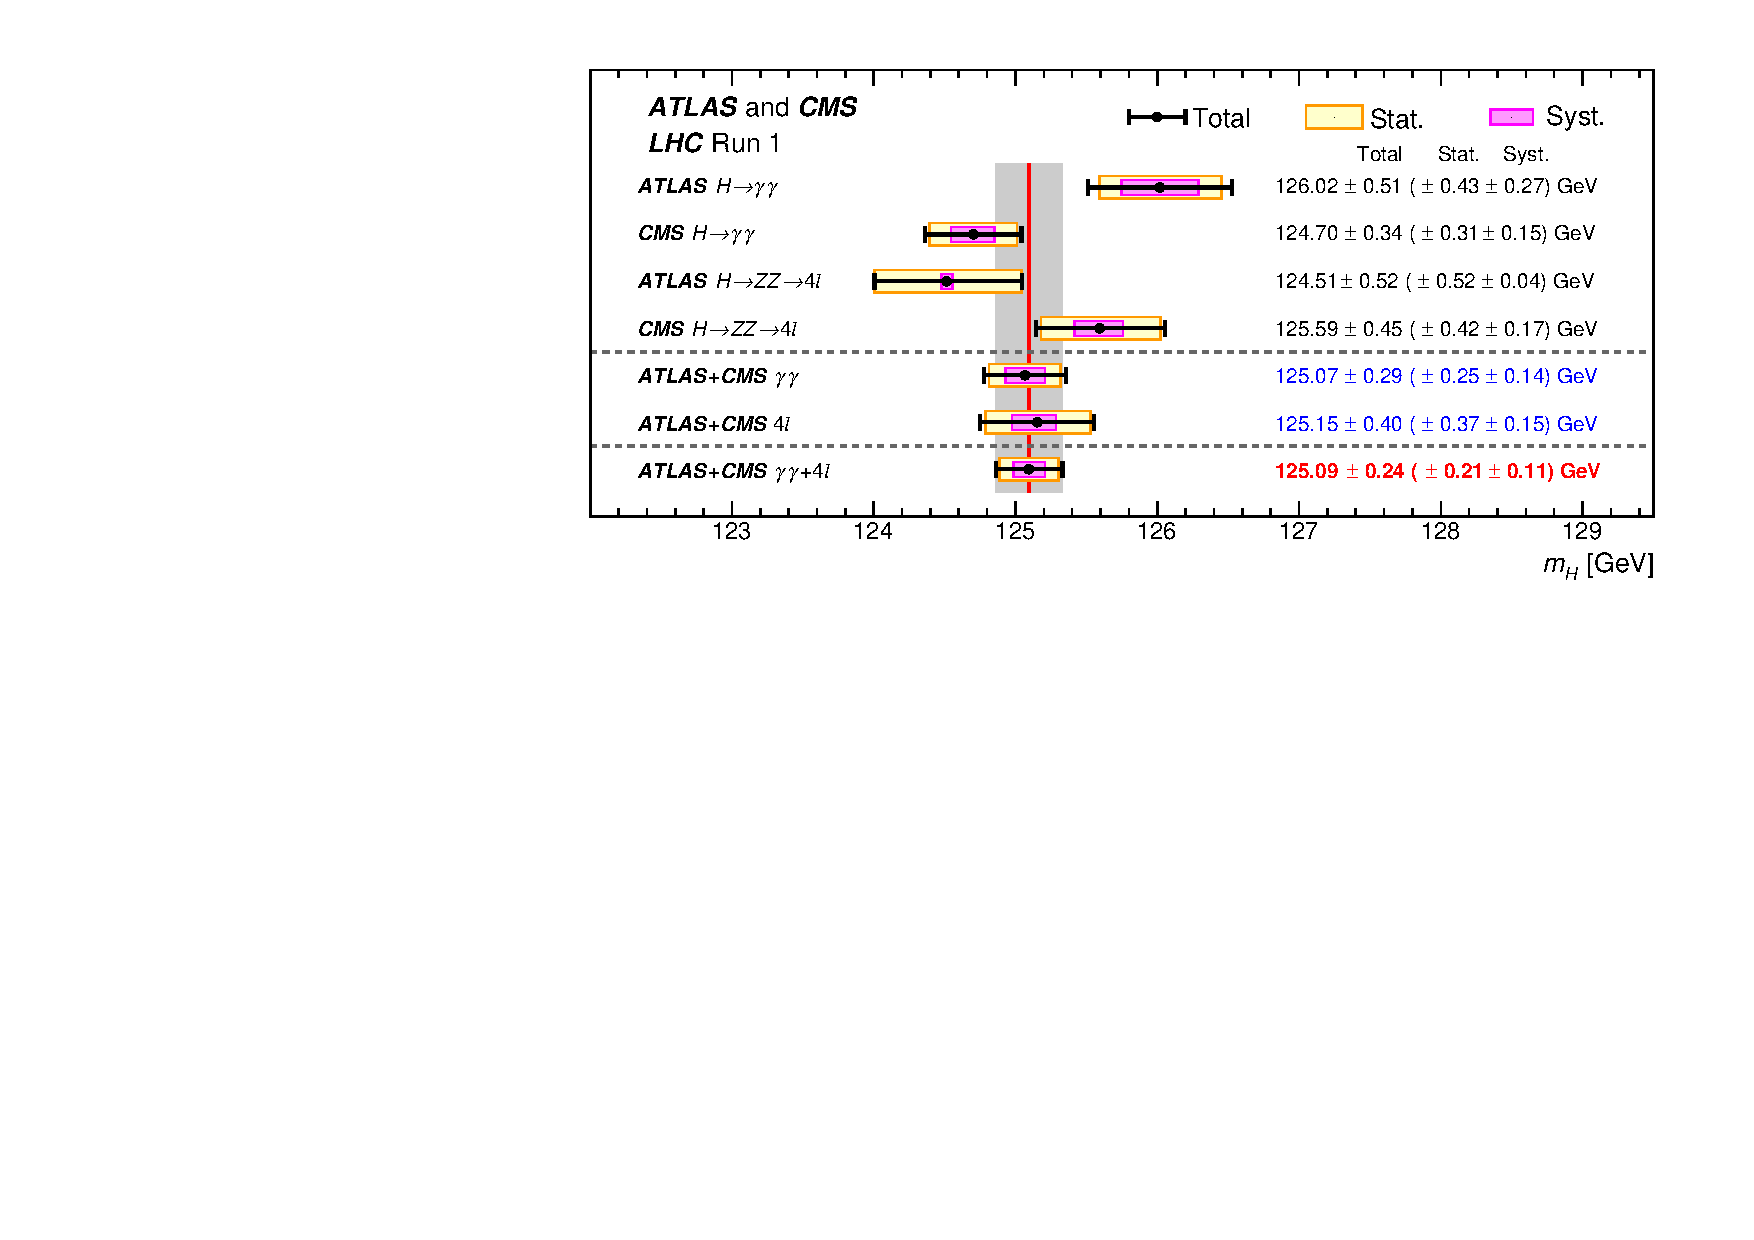
\includegraphics[width=0.8\textwidth]{figures/higgs_atlas_cms_mass}
  \caption{Resumen de las mediciones de la masa del bosón de Higgs de los
    distintos análisis de ATLAS y CMS, y del análisis combinado. Se indican las
    incertezas sistemáticas (bandas de color magenta), estadísticas (bandas de
    color amarillo), y total (lineas negras). La línea roja vertical y la
    correspondiente sombra gris indican el valor central y la incerteza total de
    la medida combinada, respectivamente\cite{HiggsMass_ATLAS_CMS}.}
  \label{fig:higgs_cms_atlas}
\end{figure}



%% QCD, el modelo partónico y la descripción de las colisiones $pp$ en el LHC
%% ---------------------------------------------------------------------------
%% * From CERN-THESIS-2011-120.pdf y tincho

La cromodinámica cuántica (QCD) \cite{Ellis:1991qj} es la teoría de campos de gauge
renormalizable que describe la interacción fuerte entre las partículas que
poseen carga de color: quarks y gluones. A diferencia del fotón en QED, los gluones,
que son los mediadores de la interacción, poseen carga de color, por lo que
pueden interactuar entre ellos, dando lugar al comportamiento inusual de la
interacción fuerte. La fuerza fuerte aumenta linealmente con la distancia entre
dos cargas. La constante de acoplamiento efectiva $\alpha_s$ depende entonces de
la distancia entre las cargas o de la escala de energía de la interacción. Se
dice que la constante ``corre'', siendo grande a bajas energía (o grandes
distancias) y haciéndose más chica a altas energías (o menores distancias).

El efecto neto de esta característica del acoplamiento fuerte es el
confinamiento, es decir, que las partículas con color no puedan existir
libremente. Solo estados de color neutro de múltiples partículas de color pueden
ser observados en la naturaleza viajando distancias macroscópicas. Los estados
que consisten en un par quark-antiquark son denominados mesones y  los
 formados por tres quarks son denominados bariones. El protón en un
barión constituido por dos quarks $u$ y uno $d$, donde cada quark tiene uno de
los tres posibles cargas de color para dejar un estado neutro. Estos tres quarks
son llamados quarks de valencia del protón, pero estos están rodeados por un mar
de gluones y pares de quark-antiquark que surgen de fluctuaciones cuánticas.
Otra consecuencia de la estructura de la interaccion fuerte es que los calculos
perturbativos no son posibles en el regimen de grandes valores de $\alpha_s$.

El LHC es un colisionador de protones, por lo tanto es esencial una precisa
descripción de la estructura del protón, ya que una colisión $pp$ a altas
energías es básicamente una colisión de dos constituyentes del mismo. Es
necesaria una descripción de los constituyentes del protón a la escala de
energía $Q$ de la dispersión fuerte.

%% A altas energías es posible entonces aplicar el llamado \emph{modelo de partones},
%% en el cual los hadrones están compuestos por partículas puntuales. Este
%% modelo fue introducido por Feynman [] y Bjorken [] a fines de los a\~nos 60,
%% para interpretar los resultados de los experimentos de dispersión profundamente
%% inelástica (DIS) electrón-nucleón en SLAC []. Esta descripción ha probado ser una buena
%% aproximación para las interacciones partón-partón de gran trasferencia de momento pero
%% no es apropiado para modelar la interacción a bajas energías.
Los quarks de valencia y los quarks y antiquarks del mar junto con los gluones
son llamados \emph{partones} del protón. Cada partón lleva solo una fracción del
momento y la energía del protón. Para la medición de una sección eficaz de
dispersión fuerte que involucre quarks y gluones en el estado inicial, es
necesario conocer el momento de las partículas incidentes. Como los partones
solo llevan una fracción del momento, y están en interacción permanente entre
ellos, el momento es desconocido, por lo que el $Q$ de las colisiones varía.
Además los quarks y gluones salientes no pueden observarse directamente debido
al confinamiento, pero entran en el detector como jets. Entonces no es posible
medir una sección eficaz partónica como $\sigma(qg \to qg)$, pero se puede hacer
una medida inclusiva, como la sección eficaz hadrónica $\sigma(pp \to jj)$ con
dos jets en el estado final. En teoría de perturbaciones, para pasar
desde la sección eficaz hadrónica a la sección eficaz partónica es necesario
conocer la probabilidad de que un partón de tipo $n$ sea encontrado con una
fracción de momento $x$, es decir, las funciones de distribución partónica
(PDF). Estas funciones son determinadas a partir de datos obtenidos de los
propios experimentos de altas energías, ya que no pueden determinarse a partir
de la teoría.

%% Esta conexion entre los hadrones observables y el nivel partónico es
%% posible gracias al concepto de \emph{factorización}, que permite una
%% separación sistemática entre las interacciones de corta distancia (de los
%% partones) y las interacciones de larga distancia (responsables del confinamineto
%% de color y la formación de hadrones). El teorema de factorizacion [] establece
%% que la sección eficaz de producción de cualquier proceso de QCD del tipo $A+B\to X$,
%% siendo $a_i(b_j)$ los constituyentes del hadrón inicial $A(B)$, puede ser expresada como:

%% \begin{equation}
%%   \sigma_{AB\to X} = \sum_{ij} \int dx_{a_i} \, dx_{b_j} f_{A/a_i} (x_{a_i}, \mu_F^2) \, f_{B/b_j} (x_{b_j}, \mu_F^2) \sigma_{a_i b_j\to X}(\mu_F^2,\mu_R^2)
%% \end{equation}
%% %
%% donde $x_i(x_j)$ es la fraccion del momento del hadron $A(B)$ que lleva el
%% parton $a_i(b_j)$ y $\sigma_{a_i b_j\to X}$ es la sección eficaz de la
%% interacción a nivel partónico, calculada a un dado orden de perturbaciones y una
%% escala de renormalización $\mu_R$. La escala de renormalización es introducida
%% para abservar las divergencias ultravioletas que aparecen en los cálculos
%% perturbativos más allá de LO.
%% Las funciones $f_{h/n}(x_n,\mu_F^2)$ son las PDF, que
%% representan la probabilidad de encontrar un partón de tipo $n$ en el hadrón $h$ con una
%% fracción de momento $x_n$, dada una escala de factorización $\mu_F$. Esta escala es un
%% parametro arbitrario introducido para tratas singularidades que aparecen en el regimen
%% no perturbativo. Estas divergencias son absrobidas, en forma similar a la renormalizacion,
%% dentro de las funciones de distribucion partonicas a la escala $\mu_F$. Si bien las
%% PDF no pueden ser determinadas perturbativamente, se puede predecir su dependencia con $Q^2$
%% por medio de las ecuaciones de evolucion DGLAP []. De esta forma, la medida experimental
%% de su forma funcional a un dado $Q_0^2$ fijo permite obtener predicciones de las PDF para
%% un amplio espectro de $Q^2$.


Todas las observaciones experimentales realizadas en LHC son compatibles con el SM a un nivel de
muy alta precisión.
La \cref{fig:sm_atlas_xs} muestra el buen acuerdo entre la
sección eficaz de algunos procesos del SM medidas por ATLAS y las predicciones
teóricas, a modo de ejemplo.

\begin{figure}[!htb]
  \centering
  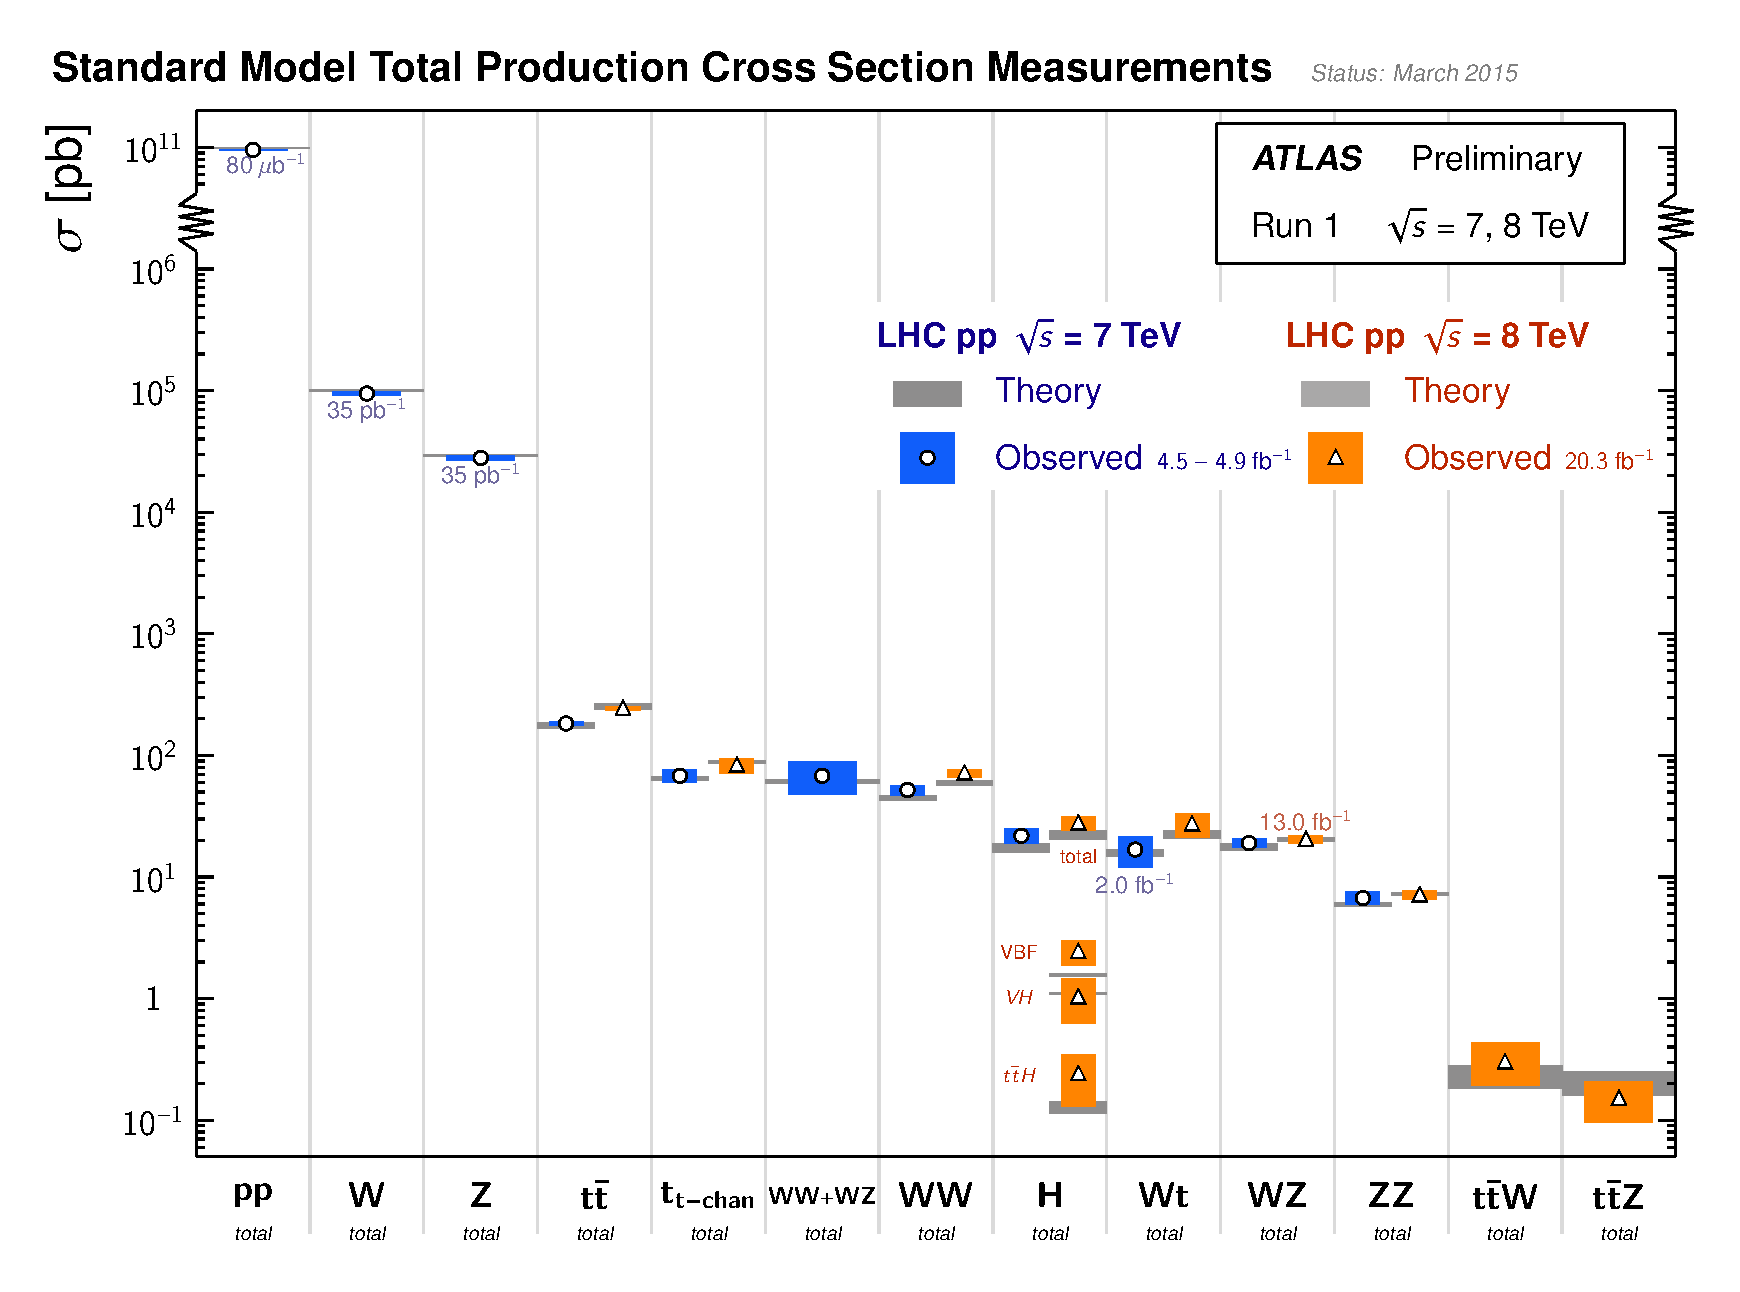
\includegraphics[width=1\textwidth]{figures/ATLAS_a_SMSummary_TotalXsect.pdf}
  \caption{Resumen de las distintas medidas de sección eficaz de producción de
    procesos del SM, comparadas con sus valores teóricos esperados.
    Los valores teóricos esperados fueron calculados como mínimo a NLO\cite{ATLASSM}.}
  \label{fig:sm_atlas_xs}
\end{figure}



\subsection{Física más allá del SM}

El SM provee una descripción extremadamente exitosa de todos los fenómenos
accesibles con los experimentos de altas energías disponibles actualmente.
Sin embargo,
también se sabe que el SM sufre de algunas debilidades, tanto desde el punto de
vista teórico, como experimental.

El hecho de que existan cuatro tipos de interacciones distintas e independientes
es un poco insatisfactorio y desde Einstein se ha especulado que estas
diferentes interacciones sean distintas manifestaciones de un único campo
unificado. El descubrimiento de los bosones $Z$ y $W$, tal como fueron predichos
por la teoría electrodébil, significaron un triunfo de la idea de una teoría unificada de las
fuerzas. Cabe destacarse que los resultados de las medidas de precisión de la sección
eficaz diferencial de las corrientes cargadas y neutras en la dispersión inelastica
profunda, obtenidos en HERA \cite{Hera}, proporcionaron una clara evidencia de la unificación
electrodébil.

Todo parece indicar que el SM es una teoría efectiva a bajas energías, muy precisa hasta
escalas de energía del orden de los 100 {\gev}. Sin embargo, los físicos
consideran que el éxito del SM no se extenderá a energías mayores. Esta
idea surge de los intentos de incorporar el SM en una teoría mas
fundamental. Incluso ante la ausencia de la gran unificación de las fuerzas
electrodébil y fuerte a una escala muy alta de energía, el SM debería ser
modificado para incorporar los efectos de la gravedad a la escala de Planck.

El SM tiene 25 (ó 26) parámetros libres. Ellos son: las masas de los doce fermiones;
las tres constantes de acoplamiento $g$, $g'$ y $g_s$; los dos parámetros que
describen el potencial de Higgs $v$ y $m_H$; y los ocho ángulos de mezcla. Y
además el Lagrangiano de QCD puede contener una fase, $\theta_{\text{CP}}$ que
experimentalmente se conoce que es $\sim 0$. Esta gran cantidad de parámetros
libres se eligen para ajustarse a los datos observados, y no provienen de
principios teóricos más fundamentales, lo cual es otro síntoma de debilidad.

En este contexto también resulta inexplicable por qué el cociente $m_W/m_P \sim
10^{-17}$ es tan chico. A esto se lo conoce como problema de \emph{jerarquía}.
Además, en el SM, la escala de las interacciones electrodébiles se derivan de un
campo escalar elemental que adquiere un valor de expectación de vacío $v = 2
m_W /g = 246 \gev$. Sin embargo, si uno acopla una teoría de partículas
escalares a nueva física a alguna escala arbitraria $\Lambda$, las correcciones
radiativas al cuadrado de la masa escalar son del orden de $\Lambda^2$, debido a
las divergencias cuadráticas en la auto-energía, lo cual indica la sensibilidad
cuadrática a la mayor escala de energía de la teoría. Por esto, la masa
``natural'' de cualquier partícula escalar es $\Lambda$. Así, para tener una teoría
electrodébil exitosa, la masa del Higgs debe ser del orden de la escala
electrodébil. Este hecho, que la masa del bosón de Higgs no puede ser igual a su
valor natural de $M_P$, es llamado del problema de \emph{naturalidad}.

Desde el punto de vista experimental, también existen algunos resultados que no
pueden acomodarse dentro del SM. El SM considera a los neutrinos como partículas
no masivas, pero distintos
experimentos\cite{PhysRevLett.101.111301,PhysRevD.78.032002} han observado
que los mismos presentan oscilaciones de sabor, lo que puede explicarse en el caso en
que estos tengan una masa no nula. Por el momento sólo existen límites
superiores para estas estas masas (ver \cref{tab:fermions}), que son muy peque\~nas
comparadas con las de los demás fermiones. El término de
masa para fermiones puede escribirse usando el doblete de Higgs si existen los
fermiones de helicidad izquierda y derecha para un dado sabor. La masa obtenida
por esta interacción es llamada masa de Dirac. Para que este mecanismo puede ser
utilizado en los neutrinos, deberían existir los neutrinos de helicidad derecha.

El SM tampoco provee un candidato para explicar la naturaleza de la materia
oscura. La existencia de la materia oscura fue inferida por primera vez como
resultado de las inconsistencias observadas entre la masa estimada de las curvas
de rotación galácticas y de su luminosidad\cite{DM1}.
Solo el 4\% del universo consiste en la materia que
conocemos\cite{DM2}, cerca del 73\% consiste en energía oscura, y el restante
23\% es materia oscura.
%% \hll{Como esta materia oscura no interactúa por medio de
%% interacciones fuerte y electromagnética, y la interacción débil es despreciable
%% en largas distancias, la materia oscura solo interactúa vía gravedad.}
La única
partícula del SM que podría ser un candidato viable de materia oscura es el
neutrino, pero como su masa es muy chica para poder explicar estos fenómenos,
puede descartarse.

%% Durante las ultimas décadas se ha intentando solucionar estos problemas.
%% Las soluciones propuestas involucran remover las
%% divergencias cuadráticas de la teoría que son la causa de los problemas de
%% jerarquía y naturalidad. Se han propuesto dos clases de soluciones. En una, los
%% escalares elementales son removidos, y por lo tanto uno debe agregar nuevos
%% fermiones y fuerzas fundamentales. Ejemplos de esto son los modelos de
%% \emph{tecnicolor} o los modelos \emph{compuestos}. La segunda clase de modelos
%% son aquellos en los que se introducen nuevas partículas al SM de forma de
%% cancelar exactamente las divergencias cuadráticas. Esta cancelación solo puede
%% ser el resultado de una nueva simetría.

Son varias las teorías que intentan explicar parcial o totalmente los problemas
mencionados anteriormente. Estas se conocen como teorías de física más allá del SM y entre
ellas se encuentra la Supersimetría, modelos con dimensiones extra, teoría de
cuerdas, teorías technicolor, etc. En el siguiente capítulo se explicará brevemente
en qué consiste una de las teorías de física más allá del SM más motivadas desde
el punto de vista teórico y experimental, que es la Supersimetría.

\section{Supersimetría}
\label{cap:susy}

Una de las teorías de física más allá del SM más motivadas desde el punto de
vista teórico es la Supersimetría, ya que resuelve algunos de los problemas
fundamentales del mismo. Entre otras cosas provee una solución al problema de
jerarquía, como así también una derivación del mecanismo de Higgs, permite la
unificación de las fuerzas del SM y hasta provee una conexión entre estas y la
gravedad, además de proporcionar un candidato para la materia oscura.

%% Sin embargo el concepto de Supersimetría no nació por estos motivos. Durante el
%% a\~no 1966 Hironari Miyazawa propuso la existencia de una supersimetría que
%% relacionaba mesones y bariones en el contexto de la física hadrónica, aunque
%% este trabajo fue ignorado en ese momento.
%% Durante 1971 y 1972 varios físicos redescubrieron la supersimetría de manera
%% independiente en el contexto de la teoría cuántica de campos, una nueva simetría
%% del espacio-tiempo y los campos fundamentales que establecía una relación entre
%% las partículas elementales con naturaleza cuántica distinta (bosones y
%% fermiones), y unificaba el espacio-tiempo con las simetrías internas de los
%% fenómenos microscópicos. Este redescubrimiento apareció ligado a las primeras
%% teorías de cuerdas.
%% Finalmente, Julius Wess y Bruno Zumino (en 1974) identificaron el carácter
%% renormalizable de la teorías de campos supersimétricas en cuatro dimensiones, y
%% luego Abdus Salam y sus estudiantes introdujeron las primeras aplicaciones para
%% física de partículas. La primera versión realista de un SM supersimétrico fue
%% propuesta durante 1977 por Pierre Fayet y se conoce como MSSM.

En esta sección se introduce el concepto de Supersimetría y se detallan algunas
características fenomenológicas que resultan importantes para esta Tesis.


\subsection{Problema de jerarquía}

El {\SM} de la física de altas energías descripto en el capítulo anterior, con
el agregado de la masa de los neutrinos, y el descubrimiento del bosón de Higgs,
ha tenido un gran éxito en la descripción de los fenómenos conocidos hasta la
escala del {\tev} explorados por los experimentos en los últimos a\~nos.
%% A pesar de esto, resulta claro que el Modelo Est\'andar no es una teoria definitiva y va a tener que
%% ser extendida para describir la f\'isica de altas energ\'ias.
A pesar de esto, no hay dudas respecto a que será necesaria una nueva teoría
a la escala reducida de Planck $M_P = (8\pi G_\text{Newton})^{-1/2} = 2.4 \times
10^{18} \gev$ , donde los efectos cuánticos gravitacionales son importantes.
Se sabe que tiene que existir nueva física en los 16 órdenes de magnitud en
energía entre el territorio explorado cerca de la escala electrodébil y la
escala de Planck. El sólo hecho de que la relación $M_P/M_W$ es tan grande es
una gran pista para la física más allá del {\SM}, por el llamado \emph{problema
  de jerarquía}. Este no es una dificultad intrínseca del SM, sino una
preocupante sensibilidad del potencial de Higgs a nueva física en casi cualquier
extensión imaginable del SM.

La parte eléctricamente neutra del campo de Higgs del SM es un escalar complejo
$H$ con un potencial clásico $V=m_H^2 |H|^2 + \lambda|H|^4$. El SM necesita un
valor de expectación del vacío (VEV) para $H$ en el mínimo del potencial no
nulo. Esto ocurre si $\lambda>0$ y $m_H^2<0$, resultando en $\avg{H} =
\sqrt{-m_H^2/2\lambda}$. Como experimentalmente sabemos que $\avg{H}$ es
aproximadamente 174 \gev, de las medidas de las propiedades de las interacciones
débiles, el valor de $m_H^2$ debe ser del orden de $-(100 \gev)^2$.

\begin{figure}[!htbp]
  \centering \begin{tikzpicture}[node distance=1cm and 1 cm]

  \coordinate[vertex, label=above:$H$] (v1);
  \coordinate[vertex, right=of v1] (v2);
  \coordinate[vertex, right=of v2] (v3);
  \coordinate[vertex, right=of v3] (v4);

  \draw[higgs] (v1) -- (v2);
  \draw[higgs] (v3) -- (v4);

  \draw[fermion] (1.5, 0) circle (0.5);
  \node at (1.5, 0.75) {$f$};

\end{tikzpicture}

  \caption{Correcciones cuánticas a un loop al parámetro de masa del Higgs
    $m_H^2$ debido a la masa de un fermión de Dirac $f$.}
  \label{fig:higgs_correction_f}
\end{figure}

El problema es que $m_H^2$ recibe grandes correcciones cuánticas de los efectos
virtuales de cada partícula que se acopla, directa o indirectamente, el
campo de Higgs. Por ejemplo, en la \cref{fig:higgs_correction_f} tenemos una
corrección a $m_H^2$ del loop que contiene un fermión de Dirac $f$ con masa
$m_f$. Si el campo de Higgs se acopla a $f$ con un término en el lagrangiano
igual a $-\lambda_f H \bar{f}f$, el diagrama de Feynman en la
\cref{fig:higgs_correction_f} genera una corrección:

\begin{equation}
  \Delta m_H^2 = -\frac{|\lambda_f|^2}{8\pi^2} \Lambda^2_{\text{UV}} %+ \ldots
  \label{eq:higgs_corr_f}
\end{equation}
%
donde $\Lambda_\text{UV}$ es el corte usado para regular la integral en el
\emph{loop}. Debe ser interpretado como la m\'inima escala de energ\'ia a la
cual entra la nueva física para alterar el comportamiento de la teoría a altas
energías. Los puntos suspensivos representan términos proporcionales a $m_f^2$,
que crecen a lo sumo logaritmicamente con $\Lambda_\text{UV}$. Cualquiera de los
leptones o quarks del SM puede jugar el rol de $f$ (para el caso de quarks la
correcciónón tiene que ser multiplicada por 3 para tener en cuenta el color) y
la correción m\'as grande va a ser cuando $f$ es el quark \emph{top} con
$\lambda_f \approx 1$.

El problema aparece si $\Lambda_\text{UV}$ es del orden de $M_P$, ya que la
corrección a $m_H^2$ es 30 órdenes de magnitud más grande que el valor requerido
de $m_H^2 \sim (100 \gev)^2$. Este es sólo un problema para las correcciones al
cuadrado de la masa del bosón de Higgs escalar, porque las correcciones
cuánticas a las masas de los fermiones y los bosones de gauge no tienen una
sensibilidad cuadrática directa a $\Lambda_\text{UV}$ como la que están en la
\cref{eq:higgs_corr_f}. Sin embargo, los quarks, leptones y los bosones de gauge
electrodébiles $Z^0$, $W^{\pm}$ del SM, todos obtienen masa de $\avg{H}$, por
lo tanto el espectro completo de masas del SM es directa o indirectamente
sensible a la escala de corte $\Lambda_\text{UV}$.

Se puede pensar que la solución es elegir un $\Lambda$ no demasiado grande, pero
igualmente se debería mezclar todavía algo de nueva física a la escala
$\Lambda_\text{UV}$ que no solo altere los propagadores en el \emph{loop}, sino que
corte la integral. Esto no es fácil en una teoría cuyo lagrangiano no contiene
mas de dos derivadas, y las teorías de mayor orden en derivadas generalmente
sufren de fallas de unitariedad o causalidad.
%In string theories, loop integrals are nevertheless cut off at high Euclidean
%% momentum p by factors e −p /Λ UV . However, then Λ UV is a string scale that
%% is usually † thought to be
%% not very far below M P . Furthermore, there are contributions similar to eq.
%% (1.2) from the virtual effects
%% of any arbitrarily heavy particles that might exist, and these involve the
%% masses of the heavy particles,
%% not just the cutoff.

\begin{figure}[!htbp]
  \centering \begin{tikzpicture}[node distance=1cm and 1 cm]

  \coordinate[vertex, label=above:$H$] (v1);
  \coordinate[vertex, right=of v1] (v2);
  \coordinate[vertex, right=of v2] (v3);
  \coordinate[vertex, right=of v3] (v4);

  \draw[higgs] (v1) -- (v2);
  \draw[higgs] (v2) -- (v3);
  \draw[higgs] (v3) -- (v4);

  \draw[higgs] (1.5, 0.5) circle (0.5);

  \node at (1.5, 1.25) {$S$};

\end{tikzpicture}

  \caption{Correcciones cuánticas a un loop al parametro de masa del Higgs
    $m_H^2$ debido a la masa de un campo escalar $S$.}
  \label{fig:higgs_correction_s}
\end{figure}

En el caso de que exista un escalar complejo pesado $S$ con masa $m_S$ que se
acopla al Higgs con un término en el Lagrangiano $-\lambda_S \abs{H}^2
\abs{S}^2$, el diagrama de Feynman es el que se muestra en la
\cref{fig:higgs_correction_s} y este da lugar a una corrección:

\begin{equation}
  \Delta m_H^2 = \frac{\lambda_S^2}{16\pi^2} \left[ \Lambda^2_\text{UV} - 2
    m_S^2 \ln (\Lambda^2_\text{UV}/m_S) + \ldots \right]
  \label{eq:higgs_corr_s}
\end{equation}

%% Puede ser que el boson de Higgs no sea una fundamenta, como en modelos technicolor, o modelos en
%% los cuales el Higgs es compuesto.
Si el bosón de Higgs es una partícula fundamental y hay física a una escala
mucho mayor que la escala electrodébil, existen dos opciones: hacer
alguna suposición bizarra de que no existe ninguna partícula de mayor masa o
efectos que se acoplen (incluso indirectamente o extremadamente débiles) con el
campo escalar de Higgs, o es necesario algún tipo de cancelación entre las
distintas contribuciones a $\Delta m_H^2$.

%------
% SUSY
%------
\subsection{Supersimetría}

La cancelación sistemática de las contribuciones a $\Delta m_H^2$ puede ser
realizada por una simetría. Comparando las
\cref{eq:higgs_corr_f,eq:higgs_corr_s} se puede ver que existe una diferencia
de signo
entre las contribuciones del \emph{loop} fermiónico y bosónico. La cancelación de todas
estas contribuciones a las masas escalares no solo es posible, sino que es
inevitable, si se considera la existencia de una simetría que relacione fermiones y
bosones. A esta simetría se la denomina supersimetría o SUSY.

Una transformación supersimétrica convierte un estado bosónico en uno
fermiónico, y viceversa. El operador $Q$ que genera estas transformaciones debe
ser un espinor anticonmutativo, con

\begin{equation}
  Q \ket{\text{bosón}} = \ket{\text{fermión}}, \quad \quad Q
  \ket{\text{fermión}} = \ket{\text{bosón}}
\end{equation}

Los espinores son intrínsecamente objetos complejos, por lo tanto el conjugado
hermitico de $Q$ es también un generador de la simetría. Debido a que $Q$ y
$Q^\dagger$ son operadores fermiónicos, llevan momento angular de espín $\frac{1}{2}$, por
lo tanto es claro que SUSY debe ser una simetría espacio-temporal y los
operadores $Q$ y $Q^\dagger$ deben satisfacer un álgebra de la siguiente forma,

\begin{align}
  \{Q, Q^\dagger\} &= P^\mu \\
  \{Q, Q\} &= \{Q^\dagger, Q^\dagger\} = 0 \\
  [P^\mu, Q] &= [P^\mu, Q^\dagger] = 0
\end{align}
%
donde $P^\mu$ es el momento generador de las traslaciones
espacio-temporales.

Los estados de partícula de una teoría supersimétrica son representados en el
álgebra de SUSY como supermultipletes. Cada supermultiplete contiene
ambos estados, fermión y bosón, que son comúnmente llamados supercompa\~neros
uno de otro.

Los generadores $Q$ y $Q^\dagger$ conmutan con los generadores de las
transformaciones de gauge, por lo tanto las partículas en un mismo
supermultiplete tienen que estar en la misma representación del grupo de gauge,
y tener la misma carga eléctrica, isospin y color. Y como el operador de masa
$-P^2$ también conmuta con los generadores y con todos los operadores de
rotación y traslación, deberán tener los mismos autovalores de $-P^2$, y
entonces la misma masa.

Es fácil probar que cada supermultiplete tiene que contener igual número de
grados de libertad fermiónico que bosónico, $n_B = n_F$. La posibilidad más
simple para satisfacer esto es tener un único fermión de Weyl ($n_F=2$) y dos
escalares reales (cada uno con $n_B=1$). Estos dos escalares se suelen poner
como un único campo escalar complejo. Esta combinación de un fermión de Weyl de
dos componentes y un campo escalar complejo es llamado un supermultiplete
quiral (ó escalar).

Otra posibilidad es que el supermultiplete contenga un bosón vectorial de espín
1. Para que la teoría sea renormalizable, tiene que ser un bosón de gauge no
masivo, al menos antes de que la simetría de gauge sea espontáneamente rota. En
este caso, este bosón contiene dos estados de helicidad, $n_B=2$. Por lo tanto
su supercompa\~nero es un fermión de Weyl de espín $\frac{1}{2}$, con dos estados de
helicidad, $n_F=2$. Si en vez de esto, se intenta usar un fermión de espín $\frac{3}{2}$
la teoría no sería renormalizable. Los bosones de gauge deben transformar como
la representación adjunta del grupo de gauge, por lo que sus compañeros
fermiónicos, llamados \emph{gauginos}, también. Esta combinación de gauginos
de espín $\frac{1}{2}$ y bosones de gauge de espín 1 es llamada supermultiplete de
gauge (ó vectorial).

Si se incluye la gravedad, el gravitón de espín 2 (con dos estados de helicidad,
$n_B=2$) tiene un supercompañero de espín $\frac{3}{2}$ llamado \emph{gravitino}.

Existen otras combinaciones posibles de partículas que pueden satisfacer estas
condiciones, pero siempre se reducen a combinaciones de supermultipletes
quirales o de gauge, excepto en ciertas teorías con supersimetría extendida.
Estas teorías tienen más de una copia de los generadores $Q$ y $Q^\dagger$, pero no
son muy prometedoras desde el punto de vista fenomenológico. La teoría no
extendida y fenomenológicamente viable es llamada generalmente $N=1$, donde $N$
se refiere al número de supersimetrías (el número de las distintas copias de
$Q$ y $Q^\dagger$).


%------
% MSSM
%------
\subsection{Modelo Mínimo Estándar Supersimétrico}

En una extensión supersimétrica del SM, cada una de las partículas fundamentales
conocidas esta contenida en un supermultiplete quiral o de gauge, y debe tener
un supercompa\~nero con espín que difiere en $\frac{1}{2}$ de este. La extensión que
requiere la introducción de la mínima cantidad de partículas se conoce como
\emph{Modelo Mínimo Estándar Supersimétrico}, o MSSM.

%% The first step in understanding the exciting phenomenological consequences of
%% this prediction is to decide exactly how the known particles fit into supermultiplets, and to give them
%% appropriate names.

Sólo los supermultipletes quirales pueden contener fermiones cuya parte
izquierda y derecha transforman de forma diferente bajo el grupo de gauge. Todos
los fermiones del SM (quarks y leptones) tienen esta propiedad, por lo tanto
deben ser miembros de supermultipletes quirales. Los nombres de los compañeros
de espín 0 de los quarks o leptones son construidos anteponiendo una ``s'' (de
\emph{scalar}), y son llamados \emph{squarks} y \emph{sleptones}, o
\emph{sfermiones}. La parte izquierda y derecha de los quarks y leptones son
fermiones de Weyl con diferentes propiedades de transformación de gauge del SM,
entonces cada uno debe tener un compañero escalar complejo. Por ejemplo, los
supercompañeros de la parte izquierda y derecha del campo de Dirac de los
electrones son llamadas {\selL} y {\selR}, aunque el subíndice no se refiere a
la helicidad de los slectrones (ya que tiene espín 0) sino a la de sus supercompañeros.
Lo mismo ocurre para {\smuL}, {\smuR}, {\stauL} y {\stauR}. Los neutrinos del SM
son siempre izquierdos por lo que sus supercompañeros se denotan {\snu}. Y
para los quarks se tiene {\squarkL} y {\squarkR}, con $q = u, d, s, c, b, t$. Las
interacciones de gauge de cada uno de los campos de squarks y sleptones son las
mismas que la de los correspondientes fermiones del SM.

El bosón escalar de Higgs debe estar en un supermultiplete quiral ya que tiene
espín 0. Dada la naturaleza de los campos quirales introducidos en la
implementación de SUSY, el campo escalar de Higgs no es suficiente para dar masa
a los fermiones de helicidad izquierda y derecha. Se debe agregar un nuevo campo
escalar para compensar. En el SM, el campo de Higgs es un doblete, y de los
cuatro grados de libertad solo uno permanece como consecuencia del rompimiento
de la simetría electrodébil, resultando en un bosón de Higgs. Los dos dobletes
de Higgs del MSSM son:

\begin{equation}
  H_u = \binom{H_u^+}{H_u^0}, \quad \quad \quad H_d = \binom{H_d^0}{H_d^-}
\end{equation}

Los bosones vectoriales del SM tienen que estar en supermultipletes de gauge.
Sus supercompañeros fermiónicos son llamados \emph{gauginos}. Las interacciones
de gauge de color $\text{SU}(3)_C$ de QCD son mediadas por el gluón, cuyo
compañero supersimétrico de espín $\frac{1}{2}$ es el \emph{gluino}. La simetría
electrodébil $\text{SU}(2)_L \times \text{U}(1)_Y$ esta asociada con los bosones
de espín 1, $W^+, W^0, W^-$ y $B^0$, cuyos compañeros de espín $\frac{1}{2}$ son $\susy{W}^+,
\susy{W}^0, \susy{W}^-$ y $\susy{B}^0$, y son llamados \emph{winos} y
\emph{bino}. Después de la ruptura de la simetría electrodébil, los auto-estados
$W^0$ y $B^0$ se mezclan para dar $Z^0$ y $\gamma$.

En la \cref{tab:sparticles} se puede ver las distintas partículas que
conforman el MSSM.


\begin{table}[ht!]
  \centering
  \begin{tabular}{x{4cm} x{4cm} x{4cm}}
    \hline
    {\bf Supermultiplete} & {\bf Bosón} & {\bf Fermión} \\ %& SU(3), SU(2), U(1) \\
    \hline
    gluon, gluino & $g$ & \gluino \\ %& 8, 1, 0 \\
    \hline
    W, wino & $W^\pm$, $W^0$  & $\winopm, \winozero$ \\ %& 1, 3, 0 \\

    B, bino &   $B$ & \bino \\ %& 1, 1, 0 \\
    \hline
    slepton, lepton & $(\snu, \susy{e})_L$ & $(\nu, e)_L$ \\%& 1, 2, -1/2 \\
    ($\times 3$ generaciones)     & $e_\mathrm{R}$ & $e_\mathrm{R}$ \\ %& 1, 1, -2 \\

    \hline

    squark, quark & $(\susy{u}_\mathrm{L}, \susy{d}_\mathrm{L})$ & $(u_\mathrm{L}, d_\mathrm{L})$ \\ %& 3, 2, 1/6 \\
    ($\times 3$ generaciones)  & $\susy{u}_\mathrm{R}$ & $u_\mathrm{R}$ \\ %& 3, 1, -2/3 \\
                  & $\susy{d}_\mathrm{R}$ & $d_\mathrm{R}$ \\ %& 3, 1, 1/3 \\

    \hline

    Higgs, higgsinos & $(H_d^0, H_d^-)$ & $(\susy{H}_d^0, \susy{H}_d^-)$ \\ %& 1, 2, -1/2 \\
                     & $(H_u^+, H_u^0)$ & $(\susy{H}_u^+, \susy{H}_u^0)$ \\ %& 1, 2, 1/2 \\

    \hline

  \end{tabular}
  \caption{Supermultipletes quirales y de gauge del MSSM.}
  \label{tab:sparticles}
\end{table}



\subsubsection{Espacio de parámetros del MSSM}

Los parámetros del MSSM se pueden describir considerando de forma separada el
sector que conserva SUSY del sector de rompimiento de SUSY
\cite{PDG,Haber:1993wf}. Primero se tienen los parámetros usuales del SM: los
acoplamientos de gauge $g_s$, $g$ y $g'$, correspondientes al grupo de gauge
SU(3), SU(2) y U(1), respectivamente. Las constantes de acoplamiento entre
fermiones y Higgs: $\lambda_u$, $\lambda_d$ y $\lambda_e$. % (correspondientes
al acoplamiento de una generación).
%de quarks y leptones izquierdos y derechos, y sus super-compa\~neros,
%a los bosones y Higgs y higgsinos).
Otro parámetro es el parámetro de masa del supercampo de Higgs $\mu$.

Los demás parámetros del MSSM aparecen de los términos de rompimiento soft de
SUSY. Estos incluyen tres parámetros de masa de los gauginos ($M_3, M_2$ y
$M_1$), cinco parámetros de masa escalares para squarks y sleptones
$M^2_{\susy{Q}}$, $M^2_{\susy{U}}$, $M^2_{\susy{D}}$, $M^2_{\susy{L}}$ y
$M^2_{\susy{E}}$, términos de interacción triliniares Higgs-squark-squark y
Higgs-slepton-slepton ($A_t$, $A_b$ y $A_\tau$), y los parámetros de masa del
sector de Higgs ($m^2_{1H}$, $m^2_{2H}$ y $m^2_{12}$). Luego del rompimiento de
la simetría electrodébil, los parámetros $m^2_{1H}$, $m^2_{2H}$ y $m^2_{12}$
pueden ser expresados en términos de dos valores de expectación del vacío ($v_1$
y $v_2$) y una masa física de Higgs (en general se elige la masa del Higgs
escalar CP-impar, $m_{A^0}$). Como $v_1^2+v_2^2=(246 \gev)^2$ esta fijo por la
masa del $W$ o $Z$, se suele escribir en términos de un parámetro definido como
el cociente $\tan \beta \equiv v_2/v_1$.

En un modelo con una sola generación de quarks, leptones y sus
supercompa\~neros, la lista anterior tiene 14 nuevos parámetros. En el modelo
completo de tres generaciones, el número de nuevos parámetros es sustancialmente
mayor ya que los parámetros de masa de los squarks y sleptones y los parámetros
$A$ serán matrices de $3 \times 3$, y la posibilidad de mezcla entre
generaciones puede llevar a complicaciones adicionales. Sin embargo, no todos
estos parámetros son físicos. Algunos de estos parámetros pueden ser eliminados
expresando los autoestados de interacción en términos de los autoestados de
masa, con la apropiada redefinición de los campos del MSSM para remover los
grados de libertad no físicos. El análisis de la referencia
\cite{Dimopoulos:1995ju} muestra que el MSSM posee 124 parámetros
independientes. De estos, 18 corresponden a los parámetros del SM, uno
corresponde al sector de Higgs (el análogo a la masa del Higgs del SM), y 105
son nuevos parámetros del modelo.

Realizar predicciones y análisis fenomenológicos con esta cantidad de parámetros
es impracticable, por lo cual es necesario realizar suposiciones para reducir
los grados de libertad. Es debido a este motivo que no existe una definición
precisa del MSSM y es importante conocer cuales son las suposiciones que se han
hecho cuando se estudia un determinado análisis.

En un tratamiento fenomenológico completo todos los parámetros del MSSM deberían
dejarse libres y determinarse a partir de los datos observados. Luego de que los
parámetros hayan sido medidos, se podría intentar extraer información de la física
subyacente que esta asociada con escalas de energía mayores a la de los
experimentos.
%%\note{Agregar límites a los parametros?}

%% Ya que la conjetura principal de SUSY esta motivada por el
%% intento de embed la física de bajas energías en un modelo más fundamental, es
%% apropiado explotar esta motivación en contraining los parámetros de SUSY a
%% bajas energías.


\subsubsection{Paridad R}

La forma general del superpotencial del MSSM tiene como inconveniente que el
número leptónico y bariónico no es una cantidad conservada. Esto implica que el
protón puede decaer a través del intercambio del compañero escalar del quark
$d$. Esto se contradice claramente con la evidencia experimental, que establece
un límite superior en la vida media del protón que es $> 10^{30}$ a\~nos a $90\%$ CL\cite{PDG}.

Para evitar este problema, la estrategia más comúnmente utilizada es introducir
una nueva simetría. Esta simetría se la conoce como paridad-R y puede escribirse
como,

\begin{equation}
  P_R = (-1)^{3(B-L)+ 2s}
\end{equation}
%
donde $B$ y $L$ son respectivamente el número bariónico y leptónico, y $s$ es el
espín de la partícula. Las partículas supersimétricas tienen $P_R = -1$, mientras
que las partículas del SM tienen $P_R = +1$.

Si la paridad-R es exactamente conservada, no puede haber mezcla entre las
spartículas y las partículas del SM. Cada vértice de interacción en la teoría
contiene entonces un número par de spartículas, lo cual conlleva a tres
consecuencias fenomenológicas de extrema importancia:

\begin{itemize}
\item En experimentos de colisionadores, las partículas supersimétricas pueden
  sólo ser producidas en número par, en general de a dos.
\item La partícula supersimétrica más liviana, llamada LSP, es estable y no tiene
  ninguna partícula con $P_R = -1$ a la cual decaer. Si
  la LSP es eléctricamente neutra, interactúa solo de forma débil con la materia
  ordinaria, y por lo tanto resulta en un candidato muy atractivo para la
  materia oscura no bariónica que es requerida por la cosmología. Desde el punto de
  vista experimental la LSP solo será visible a través de la energía faltante
  dejada en el detector.
\item Cada partícula supersimétrica que no sea la LSP debe decaer eventualmente
  en un estado que contenga un número impar de LSP (en general una).
\end{itemize}



\subsubsection{El espectro de masas del MSSM}

Una característica importante del MSSM es que las nuevas partículas, que están
listadas en la \cref{tab:sparticles}, no son necesariamente autoestados de masa
de la teoría. Después del rompimiento de la simetría electrodébil
y de la supersimetría, puede haber mezcla entre los gauginos y higgsinos, y
entre los squarks y sleptones y los Higgs escalares que tienen la misma carga
eléctrica. La única excepción es el gluino.

En el MSSM, la descripción del rompimiento de la simetría electrodébil es un
poco más complicada que en el SM debido al hecho de que hay dos dobletes
complejos de Higgs $H_u$ y $H_d$ en vez de solo uno.
Examinar los distintos autovalores de masa de la teoría, no es un análisis
trivial, ya que cualquier conjunto de partículas con los mismos números
cuánticos puede mezclarse. En las siguientes secciones se analizan los distintos
sectores del modelo.

%% \note{Explicar mínimamente el rompimiento}

%% En el MSSM los higgsinos neutros y los gauginos se mezclan para
%% formar los cuatro neutralinos:
%% \ninoone, \ninotwo, \ninothree\ y \ninofour.
%% Y de forma similar los higgsinos cargados y los winos dan lugar
%% a los dos charginos, \chinoonepm\ y \chinotwopm.

%% con un total de 8 grados de libertad, 3 de los cuales se pierden en
%% el rompimiento
%% de la simetria EW. Por lo tanto quedan 5 bosones de Higgs en el MSSM:
%% $h^0, H^0, H^+, H^-, A^0$.
%% El más liviano de los 5 es $h^0$, el cual es el más similar al del SM.

%% We have now assembled all the pieces of the MSSM.
%% To proceed, we next examine
%% the mass eigenstates of the theory. This is not a completely trivial analysis, since
%% any set of particles of a given spin, B, L and SU(3)C × U(1)EM quantum numbers
%% can mix.


\begin{itemize}\itemsep0.2cm\parskip0.2cm

\item Sector de Higgs

Los campos escalares de Higgs en el MSSM consisten en dos dobletes de
$\text{SU}(2)_\text{L}$ complejos $H_u$ y $H_d$, con 8 grados de libertad
escalares. Después del rompimiento de la simetría electrodébil, tres de estos
son bosones de Nambu-Goldstone, que se convierten en los modos longitudinales de
los bosones vectoriales $Z$ y $W^\pm$. Los restantes cinco grados de libertad
producen los cinco bosones de Higgs físicos del modelo: el par de bosones de
Higgs cargados $H^\pm$; un bosón de Higgs neutral CP-impar $A^0$; y los bosones
de Higgs neutral CP-par, $H^0,h^0$, donde por convención $h^0$ es más liviano
que $H^0$.


\item Neutralinos y Charginos %%}\label{sec:mass_NC}

Los higgsinos y los gauginos electrodébiles se mezclan entre ellos debido al
efecto del rompimiento de la simetría electrodébil. Los higgsinos neutros
($\susy{H}_u^0$ y $\susy{H}_d^0$) y los gauginos neutros (\bino, \winozero) se
combinan para formar cuatro autoestados de masa llamados \emph{neutralinos}.
Los higgsinos cargados ($\susy{H}_u^+$ y $\susy{H}_d^-$) y los winos (\winop y
\winom) se mezclan para formar dos autoestados de masa con carga $\pm 1$
llamados \emph{charginos}.

La mezcla de los gauginos y higgsinos cargados está descripta a orden árbol por la matriz de $2\times 2$:

\begin{equation}
  M_{C} = \left(
  \begin{array}{cc}
    \M{2} & \frac{1}{\sqrt{2}} g v_u \\
    \frac{1}{\sqrt{2}} g v_d & \mu \\
  \end{array}
  \right)
\end{equation}
%
la cual se debe diagonalizar para determinar los estados físicos y las masas de los charginos.
Estos dos autoestados de masa se indican con {\chinoonepm} y
{\chinotwopm} y su masa esta dada por:

\begin{equation}
  M^2_{\susy{\chi}_{1,2}} = \frac{1}{2} \left\{ M^2 + \mu^2 + 2 m_W^2 \mp
  [(M^2-\mu^2)^2 + 4 m_W^4 \cos^2 2\beta + 4 m_W^2 (M^2+\mu^2 + 2 M \mu \sin
    2\beta)]^{1/2} \right\}
\end{equation}

%% En la base de autoestados de gauge $\psi^0 = (\bino, \winozero, \susy{H_d^0}, \susy{H}_u^0)$,
%% la parte de masa del neutralino del Lagrangiano es

%% \begin{equation}
%%   \mathcal{L}_\text{neutralino mass} = -\frac{1}{2} (\psi^0)^T M_{\nino} \psi^0 + c.c.
%% \end{equation}
%% %
%% donde

En el caso de los neutralinos la matriz de masa es:

\begin{equation}
  M_{N} = \left(
  \begin{array}{cccc}
    \M{1} & 0 & -c_\beta s_W m_Z & s_\beta s_W m_Z \\
    0 & \M{2} & c_\beta c_W m_Z & -s_\beta c_W m_Z \\
    -c_\beta s_W m_Z & c_\beta c_W m_Z & 0 & -\mu \\
    s_\beta s_W m_Z & s_\beta -c_W m_Z & -\mu & 0 \\
  \end{array}
  \right)
\end{equation}

Para el caso de los neutralinos se utiliza la siguiente notación $\tilde{\chi}^0_{i}$ ($i=1,2,3,4$)
y al igual que en el caso de los charginos son ordenados de forma ascendente según su masa (es decir,
el $i=1$ es el más liviano).

%% El neutralino más liviano
%% {\ninoone}, suele ser la LSP, salvo que exista un {\gravino} más liviano
%% o que la paridad-R no se conserve.

%% Los autoestados de masas y la matriz de mezcla $N_{ij}$ pueden obtenerse en termino de los parámetros
%% \M{1}, \M{2}, $\mu$ y $\tan\beta$.

%% El sector de los neutralinos esta determinado por tres parámetros reales, \M{1}, $\tan\beta$ y
%% $\mu$ (como también por supuesto $m_Z$ y $\theta_W$).

Si un estado de chargino o neutralino se aproxima a un estado particular de
gaugino o higgsino, es conveniente usar la nomenclatura correspondiente. Si
$M_1$ y $M_2$ son pequeñas comparadas a $m_Z$ y $|\mu|$, el neutralino más
liviano va a ser puramente fotino. Si $M_1$ y $m_Z$ son pequeños comparados a
$M_2$ y $|\mu|$, entonces el neutralino más liviano va a ser puramente bino. Si
$M_2$ y $m_Z$ son pequeñas comparadas con $M_1$ y $|\mu|$, el par de charginos
más liviano y neutralino va a constituir un triplete de winos puro degenerado en
masas. Finalmente, si $|\mu|$ y $m_Z$ son chicos comparados con $M_1$ y $M_2$,
el neutralino más liviano va a ser un higgsino puro. Cada unos de los casos
anteriores va a llevar a un fenomenología muy distinta.


\item Gluino

Como el gluino es un fermión de color con ocho componentes, no puede mezclarse con ninguna
otra partícula del MSSM (aunque haya violación de paridad-R). El parámetro de
masa del gluino $M_3$ esta relacionado con los parámetros de masa de bino y wino
($M_1$ y $M_2$) por la siguiente aproximación:

\begin{equation}
  M_3 : M_2 : M_1 \quad \sim \quad 6 : 2 : 1
\end{equation}
%
valida cerca de la escala del {\tev} (suponiendo que tienen un valor de masa común
en la escala GUT). Por este motivo es razonable considerar que el gluino es
considerablemente más pesado que los neutralinos y charginos.


\item Squarks y sleptones

Cualquier par de escalares con la misma carga eléctrica, paridad-R y color
pueden mezclarse entre ellos. Después del agregado de los términos del
rompimiento soft de la supersimetría, los auto-estados de masa de los squarks y
sleptones del MSSM pueden obtenerse diagonalizando tres matrices de $6\times6$
para squarks up, down y sleptones cargados, y una matriz adicional de $3\times
3$ para los sneutrinos. La primera y segunda familia de squarks y sleptones
terminan con siete pares casi degenerados. En contraste, la tercera familia de
squarks y sleptones pueden tener masas muy distintas y una mezcla importante de
a pares $(\stopL, \stopR)$, $(\sbottomL, \sbottomR)$ y $(\stauL, \stauR)$.

Para un cierto fermión $f$ de la tercera generación, las matrices hermiticas en
la base de los auto-estados de gauge $(\sfermionL, \sfermionR)$ pueden ser
diagonalizadas por una matriz unitaria para dar los auto-estados de masa
denotados por $(\sfermionone, \sfermiontwo)$:

\begin{equation}
  m_{\widetilde{f}_{\mathrm{1,2}}}^2 = m^2_f + \frac{1}{2} \left[
    m_{\sfermionL}^2 + m_{\sfermionR}^2 \mp \sqrt{(m_{\sfermionL}^2 -
      m_{\sfermionR}^2)^2 + 4 m_f^2 C^2} \right]
\end{equation}
%
con $m_{\sfermionone}^2 < m_{\sfermiontwo}^2$, donde el parámetro $C$ es un
valor conocido que puede ser obtenido de los acoplamientos Yukava y soft y el
cociente de los VEVs de los $H_u^0$ y $H_d^0$. Dado que la masa del top $m_t$ es
muy alta, la mezcla es particularmente importante para el sector del $\stop$.
Esto genera una gran diferencia entre las masas de los dos auto-estados de los
stops, dejando posiblemente un stop mucho más liviano a los demás squarks.

\end{itemize}


\subsubsection{Decaimiento de spartículas}

\begin{itemize}\itemsep0.2cm\parskip0.2cm

\item Neutralinos y charginos

Como cada neutralino y chargino contiene al menos una mezcla de los gauginos
electrodébiles {\bino}, $\tilde W^0$ o $\susy{W}^{\pm}$ , heredan los
acoplamientos de intensidad electrodébil a los pares de fermiones escalares. Si
los sleptones o squarks son lo suficientemente livianos, un neutralino o
chargino va a decaer a un par leptón+slepton o quark+squark. También pueden
decaer en un neutralino o chargino más liviano y un Higgs escalar o un bosón
de gauge electrodébil. Los posibles decaimientos son

\begin{align*}
  &\susy{N}_i \to Z \susy{N}_j, \quad W \susy{C}_j, \quad h^0 \susy{N}_j, \quad
  \ell \susy{\ell}, \quad \nu \susy{\nu}, \quad [A^0 \susy{N}_j, \quad H^0
    \susy{N}_j, \quad H^{\pm} \susy{C}_j^{\mp}, \quad q \susy{q}],
  \\ &\susy{C}_i \to W \susy{N}_j, \quad Z \susy{C}_1, \quad h^0 \susy{C}_1,
  \quad \ell \susy{\nu}, \quad \nu \susy{\ell}, \quad [A^0 \susy{C}_1, \quad H^0
    \susy{C}_1, \quad H^{\pm} \susy{N}_j, \quad q \susy{q}']
\end{align*}
%
donde los estados finales entre corchetes son los cinemáticamente menos
probables.


\item Sleptones

Los sleptones puede decaer en un lepton y un chargino o neutralino,

\begin{align}
  \slepton &\to \ell \nino, \nu\chinopm \\ \snu &\to \nu\nino, \ell\chinopm
\end{align}

Como los sleptones derechos no se acoplan al gaugino de $\text{SU}(2)_\text{L}$,
comúnmente prefieren el decaimiento directo a $\ell\ninoone$.


\item Gluino

El gluino solo puede decaer a través de un squark, ya sea on-shell o virtual. Si
el decaimiento a dos cuerpos está abierto, este va a dominar debido al
acoplamiento gluino-quark-squark tiene intensidad QCD. En el caso de que todos
los squarks sean más pesados que el gluino, este va a decaer sólo vía squarks
virtuales.

\begin{align}
  &\gluino \to q\susy{q}, \\
  &\gluino \to qq\nino, qq^\prime \chinopm
\end{align}


\item Squarks

Los squarks puede tener decaimiento a dos cuerpos en un squark-gluino si es
cinematicamente permitido, porque tiene acoplamiento QCD. Por otro
lado, los squarks pueden decaer en un quark y un neutralino/chargino.

\begin{equation}
  \susy{q} \to q\gluino, \, q\nino, \, q^\prime \chinopm
\end{equation}

%% El gluino, chargino o neutralino que resulta del decaimiento de un squark
%% va a decaer
%% The gluino, chargino or neutralino resulting from the squark decay will in turn
%% decay, and so on, until a final state containing χ  ̃ 1 is reached. This results in
%% numerous and complicated decay chain possibilities called cascade decays.

\end{itemize}

%---------------------
% Rompimiento de SUSY
%---------------------
\subsection{Rompimiento de la Supersimetría}

Los supermultipletes quirales y de gauge de la \cref{tab:sparticles} conforman
el contenido de partículas del MSSM. Desde el punto de vista experimental,
ninguna de las compa\~neras supersimétricas de las partículas del SM han sido
observadas hasta el momento. Si la supersimetría no estuviera rota, deberían
existir selectrones con una masa igual a $m_e \sim 0.511 \mev$, y lo mismo para
los demás sleptones y squarks. Y también deberían existir los gluinos y fotinos
sin masa. El hecho de que no hayan sido descubiertas hasta el momento es motivo
evidente de que SUSY es una simetría que esta rota en el estado de vacío elegido
por la naturaleza.

Pero una de las principales motivaciones para introducir esta nueva simetría fue
que las divergencias cuadráticas en el cuadrado de las masas escalares podían
anularse a todo orden en teoría de perturbaciones, y eso está garantizado solo
si esta simetría no esta rota. Para que SUSY todavía pueda proveer la solución
al problema de jerarquía incluso en presencia del rompimiento de esta, las
relaciones entre los acoplamientos adimensionales que están en la teoría antes
del rompimiento deben mantenerse. Para que esto suceda, el rompimiento de la
supersimetría debe ser \emph{soft}, es decir, el Lagrangiano efectivo del MSSM
tiene que poder ser escrito como:

\begin{equation}
  \mathcal{L} = \mathcal{L}_\text{SUSY} + \mathcal{L}_\text{soft}
\end{equation}
%
donde $\mathcal{L}_\text{SUSY}$ contiene todas las interacciones de gauge y de
Yukawa y preserva la invarianza supersimétricas, y $\mathcal{L}_\text{soft}$
viola supersimetría pero contiene solo términos de masa y parámetros de
acoplamientos con dimensión de masa positiva. Si la escala de masa más grande
asociada con los términos soft se llama $m_\text{soft}$, las correcciones
adicionales no supersimétricas al cuadrado de la masa escalar del Higgs debe
anularse en el límite $m_\text{soft} \to 0$.

Debido a que la diferencia de masas entre las partículas conocidas del SM y sus
súper-compañeras son determinadas por los parámetros $m_\text{soft}$ que
aparecen en $\mathcal{L}_\text{soft}$, las masas de las partículas
supersimétricas no pueden ser demasiado grandes. De otra forma perderíamos la
solución al problema de jerarquía.

Por otro lado, también existe una razón por la cual las partículas
supersimétricas deben ser lo suficientemente pesadas para no haber sido
descubiertas hasta ahora. Todas las demás partículas del MSSM que han sido
observadas tienen algo en común: deberían no tener masa en ausencia del
rompimiento de la simetría electrodébil. En particular, las masas de los
bosones $W^\pm$, $Z^0$ y todos los quarks y leptones son iguales al producto de
constantes de acoplamiento adimensionales por el $\avg{H} \sim 174 \gev$,
mientras que el fotón y el gluon necesitan ser no masivos por la invarianza de
gauge electromagnética y de QCD. Por el contrario, todas las partículas del MSSM
no descubiertas tienen la propiedad contraria. Cada una de ellas pueden tener un
término de masa en el Lagrangiano en ausencia del rompimiento de la simetría
electrodébil.

En el MSSM, el rompimiento de SUSY es introducido explícitamente. El rompimiento
de una simetría global siempre implica un modo no masivo de Nambu-Goldstone con
los mismos números cuánticos que el generador de la simetría rota. En el caso de
la supersimetría global, el generador es la carga fermionica $Q_\alpha$, por lo
tanto la partícula de Nambu-Goldstone tiene que ser un fermión de Weyl no masivo
neutro, llamado \emph{goldstino}. Es claro ahora que el rompimiento espontáneo
de la supersimetría requiere la extensión del MSSM. El rompimiento espontáneo de
SUSY tiene que ocurrir en un \emph{sector oculto} de partículas que no tienen
acoplamientos directos con los supermultipletes quirales (\emph{sector visible})
del MSSM. Sin embargo, estos dos sectores comparten algunas interacciones que
son las responsables de mediar el rompimiento de la supersimetría desde el
sector oculto al visible, resultando en los términos soft del MSSM (ver
\cref{fig:susy_breaking}).

\begin{figure}[!htbp]
  \centering
  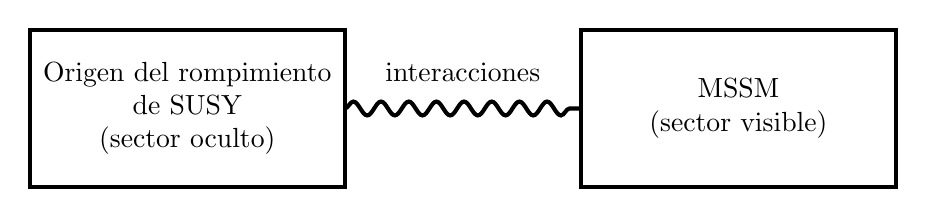
\begin{tikzpicture}

  \draw[line width=1.5] (0,0) rectangle (4,2) node[midway,align=center] (r1) {Origen del rompimiento\\ de SUSY\\ (sector oculto)};
  \draw[line width=1.5] (7,0) rectangle (11,2) node[midway, align=center] (r2) {MSSM\\ (sector visible)} ;

  \draw[line width=1.5,decorate,decoration={snake}] (4,1) -- (7,1) node[midway,above=.2cm] {interacciones};

\end{tikzpicture}

  \caption{Esquema de la supuesta estructura del rompimiento de supersimetría.}\label{fig:susy_breaking}
\end{figure}

Existen muchas propuestas de como estas interacciones mediadores pueden ser. Una
de ellas (e históricamente la más popular) es que estas interacciones son
gravitacionales (mSUGRA).

%% Más precisamente
%% estas asociados con la nueva física, incluyendo a la gravedad, que
%% aparece cerca de la escala de Planck. En este escenario

Una segunda posibilidad es que estas interacciones mediadores sean las
interacciones de gauge electrodébiles y QCD ordinarias. En estos escenarios
donde el rompimiento de supersimetría esta mediado por campos de gauge
(\emph{Gauge-mediated supersymmetry breaking} ó GMSB), los términos soft del
MSSM provienen de diagramas a un loop que involucran algunas partículas
mensajeras.

Si tenemos en cuenta a la gravedad, SUSY tiene que ser promovida a una simetría
local. Esta teoría supersimétrica local es llamada \emph{supergravedad}. Esto
unifica necesariamente las simetrías espacio-temporales ordinarias de la
Relatividad General con las transformaciones locales supersimétricas. En esta
teoría, el graviton de espín 2, tiene un supercompa\~nero fermión de espín 3/2
llamado \emph{gravitino}. Mientras la supersimetría no esté rota, el gravitón y
el gravitino son no masivos con dos estados de helicidad de espín. Una vez que
SUSY es espontáneamente rota, el gravitino adquiere una masa absorbiendo el
goldstino, que se convierte en sus componentes longitudinales (helicidad $\pm
1/2$). Este mecanismo es llamado \emph{super-Higgs}, y es el análogo al
mecanismo de Higgs ordinario de las teorías de gauge, donde los bosones de gauge
$W^\pm$ y $Z^0$ en el {\SM} adquieren masa absorbiendo los bosones de
Nambu-Goldstone asociados con la invarianza de gauge electrodébil
espontáneamente rota. La masa del gravitino es tradicionalmente llamada
$m_{3/2}$, y puede ser estimada como

\begin{equation}
  m_{3/2} \sim \avg{F} / M_P
\end{equation}
%
donde $F$ esta relacionada a la escala del rompimiento de SUSY. Esto implica
distintos valores esperados para la masa del gravitino dependiendo el modelo de
mediadores propuesto. En modelos de mediación por gravedad, la masa del
gravitino es comparable a la masa de las partículas del MSSM, por lo tanto es
esperado que sea de al menos el orden de 100 \gev. Sus interacciones van a ser
de intensidad gravitacional, el gravitino no juega ningún rol en física de
colisionadores, pero puede ser importante en cosmología.

En contraste, los modelos GMSB predicen un gravitino mucho más liviano que las
spartículas del MSSM.%% si $M_\text{mess} \ll M_P$.
En este caso, el gravitino es
la LSP, y todas las sparticulas del MSSM van a decaer eventualmente en un estado
final que incluye al gravitino.


%------
% GMSB
%------
\subsection{GMSB y GGM} %%Modelos de rompimiento de supersimetría mediados por campos de Gauge}

En los modelos de rompimiento de la supersimetría mediado por campos de gauge ó
GMSB, las interacciones ordinarias de gauge son las responsables de la aparición
del rompimiento soft de la supersimetría en el MSSM.

%% La idea básica es introducir
%% nuevos supermultipletes quirales, llamados mensajeros, que se acoplen ...
%% \note{Referencia: arxiv:9801271}

La mediación por campos de gauge es una de las maneras más simples y robustas
para transmitir el rompimiento de SUSY al MSSM. A pesar de su simpleza, existe
un gran número de modelos de GMSB. Para poder hacer un análisis fenomenológico
dentro del marco de GMSB de una forma no tan dependiente del modelo, pero con un
correcta base teórica, en \cite{GGM} se propone un marco lo más general posible
para describir los efectos de un sector oculto arbitrario, definiendo al
mecanismo de mediación por campos de gauge como: \emph{el límite en que las
  constantes de acoplamiento del MSSM $\alpha_i \to 0$, la teoría se desacopla
  en el MSSM y un sector oculto separado que rompe SUSY.}

A este marco general se lo conoce como \emph{General Gauge Mediation} ó GGM. El
conjunto de parámetros independientes de GGM esta compuesto por las tres masas
complejas de gauginos $M_1$, $M_2$ y $M_3$, y tres parámetros reales que
controlan las masas de los 5 sfermiones $m^2_{Q,U,D,L,E}$. Además los términos
trilineares $A$ siempre son pequeños.

Estos modelos ofrecen una rica variedad de estados finales en colisionadores
\cite{0911.4130}. La característica más destacable de estos modelos es el
gravitino liviano $m_{3/2} = M_\text{weak}$. La masa del gravitino en modelos
GGM es típicamente del orden del eV (en algunos casos puede llegar al \gev), lo
cual implica que el {\gravino} es la LSP. Esto asegura que los efectos de
mediación por campos de gauge domine por sobre la mediación por gravedad.

Uno de los aspectos teóricos interesantes de SUSY es que si esta simetría es
realizada como una simetría local, incorpora de forma necesaria y automática la
gravedad.
%% Esta conexión no tiene ninguna consecuencia en la mayor parte de la
%% fenomenología en colisionadores, porque las interacciones gravitatorias no son
%% relevantes. Sin embargo, esto no necesariamente cierto si el gravitino es muy
%% liviano.
%% El gravitino obtiene su masa absorbiendo el goldstino de espín 1/2 asociado al
%% rompimiento espontáneo de la supersimetría. En el límite de altas energías, las
%% interacciones de las componentes de helicidad $\pm 1/2$ del gravitino son las
%% mismas que las del goldstino.
%% Estas interacciones son proporcionales a $1/m_{\gravino}$ en el límite
%% $m_{\gravino} \to 0$ y son potencialmente importantes incluso para procesos a
%% energías ordinarias. Sin embargo, la intensidad de las interacciones del
%% gravitino no puede ser arbitrariamente grande.
La masa del gravitino esta relacionada con la escala del rompimiento de SUSY por,

\begin{equation}
  m_{\gravino} = \frac{\Lambda^2_{\text{SUSY}}}{\sqrt{3}M_P}
\end{equation}

La escala $\Lambda_{\text{SUSY}}$ tiene que ser al menos la masa de las
partículas supersimétricas más pesadas. Si consideramos que
$\Lambda_{\text{SUSY}} > 1 \tev$ entonces $m_{\gravino} > 10^{-4} \eV$.
Y por otro lado, los límites cosmológicos \cite{PhysRevLett.48.223,Moroi:1993mb}
bajo ciertas condiciones, ponen un límite superior $m_{\gravino} < 10^4 \eV$.%% , al menos en ausencia
%% de \hl{late inflation}.

El hecho de que la LSP sea siempre el gravitino, determina que la partícula mas
liviana del MSSM es entonces la NLSP, y siempre decae a un gravitino y su
compañero del SM. Como este decaimiento esta altamente suprimido por la escala
de rompimiento de SUSY, la NLSP puede decaer de forma inmediata (\emph{promtp}) o luego de haber
atravesado una cierta distancia en el detector. En lo que sigue sólo nos concentraremos
en decaimientos \emph{prompt}.
Esta supresión de la tasa de decaimiento también significa que todas las
spartículas pesadas decaen pasando por la NLSP antes de decaer en un gravitino.
Es por este motivo que la naturaleza de la NLSP es el aspecto más importante del
espectro de GMSB para los estados finales en colisionadores.


La topología típica de un evento GGM esta ilustrada en la
\cref{fig:ggm_event}, en la cual se pueden observar varias caracteristicas
importantes. El gravitino siempre va a escapar del detector, dejando una
cantidad significativa de energía faltante. Mientras tanto, el compañero del SM
va a tender a ser central y energético (asumiendo que la NLSP decae dentro del
detector), ya que es en general mucho más liviano que la NLSP. Dado que en cada
evento SUSY se producen dos NLSPs, es claro que las partículas producidas en un
colisionador van a estar determinadas por la naturaleza de la NLSP.

\begin{figure}[!htbp]
  \centering
  %%\includegraphics[width=0.5\textwidth]{figures/ggm_event}
  %\usetikzlibrary{positioning}
\usetikzlibrary{arrows}
\usetikzlibrary{patterns}
\usetikzlibrary{decorations.markings}
\usetikzlibrary{calc}
\usetikzlibrary{decorations}
\usetikzlibrary{decorations.pathmorphing}


\makeatletter

% gluon decoration (based on the original coil decoration)
\pgfdeclaredecoration{coilgluon}{coil}
{
  \state{coil}[switch if less than=%
    0.5\pgfdecorationsegmentlength+%>
    \pgfdecorationsegmentaspect\pgfdecorationsegmentamplitude+%
    \pgfdecorationsegmentaspect\pgfdecorationsegmentamplitude to last,
    width=+\pgfdecorationsegmentlength]
        {
          \pgfpathcurveto
              {\pgfpoint@oncoil{0    }{ 0.555}{1}}
              {\pgfpoint@oncoil{0.445}{ 1    }{2}}
              {\pgfpoint@oncoil{1    }{ 1    }{3}}
              \pgfpathcurveto
                  {\pgfpoint@oncoil{1.555}{ 1    }{4}}
                  {\pgfpoint@oncoil{2    }{ 0.555}{5}}
                  {\pgfpoint@oncoil{2    }{ 0    }{6}}
                  \pgfpathcurveto
                      {\pgfpoint@oncoil{2    }{-0.555}{7}}
                      {\pgfpoint@oncoil{1.555}{-1    }{8}}
                      {\pgfpoint@oncoil{1    }{-1    }{9}}
                      \pgfpathcurveto
                          {\pgfpoint@oncoil{0.445}{-1    }{10}}
                          {\pgfpoint@oncoil{0    }{-0.555}{11}}
                          {\pgfpoint@oncoil{0    }{ 0    }{12}}
        }
        \state{last}[next state=final]
              {
                \pgfpathcurveto
                    {\pgfpoint@oncoil{0    }{ 0.555}{1}}
                    {\pgfpoint@oncoil{0.445}{ 1    }{2}}
                    {\pgfpoint@oncoil{1    }{ 1    }{3}}
                    \pgfpathcurveto
                        {\pgfpoint@oncoil{1.555}{ 1    }{4}}
                        {\pgfpoint@oncoil{2    }{ 0.555}{5}}
                        {\pgfpoint@oncoil{2    }{ 0    }{6}}
              }
              \state{final}{}
}

\def\pgfpoint@oncoil#1#2#3{%
  \pgf@x=#1\pgfdecorationsegmentamplitude%
  \pgf@x=\pgfdecorationsegmentaspect\pgf@x%
  \pgf@y=#2\pgfdecorationsegmentamplitude%
  \pgf@xa=0.083333333333\pgfdecorationsegmentlength%
  \advance\pgf@x by#3\pgf@xa%
}

\makeatother

\tikzset{
  proton/.style={line width=1pt,preaction={preaction={draw,line width=5pt},draw,white,line width=3pt}},
  photon/.style={decorate, decoration={snake}, draw=black},
  higgs/.style={draw, dashed},
  fermion/.style={draw=black, postaction={decorate},decoration={markings}},
  gluon/.style ={decorate, decoration={coilgluon,amplitude=4pt, segment length=5pt}},
  gluino/.style={decorate, decoration={coilgluon,amplitude=4pt, segment length=5pt}, preaction={draw}},
  vertex/.style={draw,shape=circle,fill=black,minimum size=0pt,inner sep=0pt},
}

%% \semiloop[fermion][<draw options>]{<first node>}{<second node>}{<angle>}[<label>][<below, default: above>];
%% \NewDocumentCommand\semiloop{O{black}mmmO{}O{above}}
%% {%
%%   \draw[#1] let \p1 = ($(#3)-(#2)$) in (#3) arc (#4:({#4+180}):({0.5*veclen(\x1,\y1)})node[midway, #6] {#5};)
%% }

\colorlet{red}{red!60}
\colorlet{blue}{blue!60}
\colorlet{green}{green!60}
\colorlet{blue}{blue!50!black!70}
\colorlet{green}{green!50!black!70}
\colorlet{purple}{purple!90!black!70}
\colorlet{gray1}{black!10}

\tikzset{
    arr/.style={line width=1,
      decoration={markings,mark=at position 1 with {\arrow[scale=1.5]{>}}},
      postaction={decorate}
      },
    rec/.style={rectangle,
                fill, black,
                fill=gray1,
                very thick,
                text width=2.7cm,
                minimum height=1.5cm,
                text centered}
}


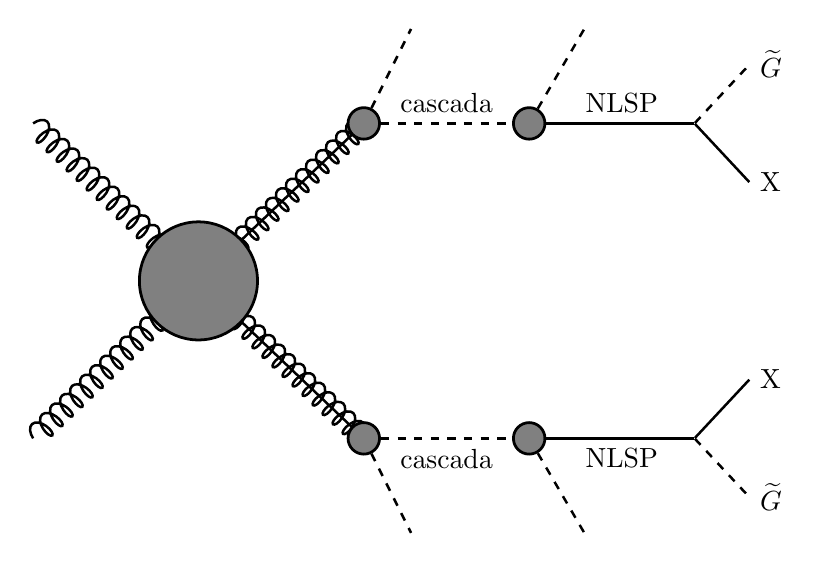
\begin{tikzpicture}

	\tikzset{
    		line/.style={line width=0.9},
    		dline/.style={dashed,line width=0.9},
  	}

	\definecolor{blue1}{HTML}{3F66BD}
	\definecolor{blue2}{HTML}{2C4784}

	\coordinate[vertex] (O) at (0,0);

	\coordinate[vertex] (C1) at (2.1, 2);
	\coordinate[vertex] (C2) at (2.1,-2);

	\coordinate[vertex] (N1_a) at (4.2, 2);
	\coordinate[vertex] (N2_a) at (4.2,-2);

	\coordinate[vertex] (N1_b) at (6.3, 2);
	\coordinate[vertex] (N2_b) at (6.3,-2);

	\coordinate[vertex] (G1) at (7, 2.75);
	\coordinate[vertex] (X1) at (7, 1.25);

	\coordinate[vertex] (G2) at (7,-2.75);
	\coordinate[vertex] (X2) at (7,-1.25);

	\draw[line,gluon] (-2.1,-2) -- (O);
	\draw[line,gluon] (-2.1, 2) -- (O);

	\draw[line] (O) -- (C1);
	\draw[line] (O) -- (C2);
	\draw[line,gluino] (O) -- (C1);
	\draw[line,gluino] (O) -- (C2);

	\draw[line] (4.0, 2) -- (N1_b) node[above, pos=.6] {NLSP};
	\draw[line] (4.0,-2) -- (N2_b) node[below, pos=.6] {NLSP};

	\draw[dline] (N1_b) -- (G1) node[right] {$\widetilde{G}$};
	\draw[line] (N1_b) -- (X1) node[right] {X};

	\draw[dline] (N2_b) -- (G2) node[right] {$\widetilde{G}$};
	\draw[line] (N2_b) -- (X2) node[right] {X};

    	\draw[black, line width=1, fill=gray] (O) circle (0.75cm); 

  	\draw[dline,fill=white] (C1) -- (N1_a) node[black,above,pos=.5] {cascada};
  	\draw[dline,fill=white] (C2) -- (N2_a) node[black,below,pos=.5] {cascada};

	\draw[dline] (C1) -- (2.7, 3.2);
	\draw[dline] (C2) -- (2.7,-3.2);
	\draw[dline] (N1_a) -- (4.9, 3.2);
	\draw[dline] (N2_a) -- (4.9,-3.2);


	\draw[black, line width=1,fill=gray] (C1) circle (0.20cm);
	\draw[black, line width=1,fill=gray] (C2) circle (0.20cm);
	\draw[black, line width=1,fill=gray] (N1_a) circle (0.20cm);
	\draw[black, line width=1,fill=gray] (N2_a) circle (0.20cm);

\end{tikzpicture}

  \caption{Esquema de la topología típica de un evento GGM en un colisionador de hadrones.
    En la interaccion fuerte se produce un par de gluinos que luego decaen en forma de cascada,
    hasta llegar a la NLSP, que decae en un gravitino {\gravino} y su companero del SM ($X$). Los
    gravitinos escapan el detector dejando un gran cantidad de energia faltante.}
  \label{fig:ggm_event}
\end{figure}


%%\subsection{Gravitino LSP}

%% Como resultado del rompimiento espontaneo de la supersimetria,
%% el espectro fisico contiene un fermion no masivo de spin 1/2,
%% el goldstino. Cuando la teoria supersimetrica global esta acoplada
%% a la gravedad y promocionada a una teoria supersimetrica local,
%% el goldstino provee los modos longitudinales de spin 3/2 del graviton:
%% el gravitino.
%% Como resultado de este mecanismo de super-Higgs, el gravitino adquiere una masa
%% que bajo la condicion de la anulacion de la constante cosmologica esta dada por:

%% \begin{equation}
%%   m_{3/2} = \frac{F_0}{\sqrt{3}M_P}
%% \end{equation}
%% %
%% donde $M_P = (8\pi G_N)^{-1/2} = 2.4 \times 10^{18} \gev$ es la masa reducida de Planck.
%% Y $F_0$ es la contribucion total del VEV de rompimiento de SUSY de los campos auxiliares
%% normalizado de tal forma que la energia de vacio de la teoria supersimetrica global es
%% $V = F_0^2$...

%% En los modelos GMSB, el gravitino es la particula supersimetrica más liviana (LSP) para
%% cualquier valor relevante de $F$. Si la paridad-R es conservada, todas las particulas
%% supersimetricas van a seguir cadenas de decaimineto que terminan en gravitinos.

%% There is then still a window of
%% perhaps 9 orders of magnitude for the mass of a light gravitino. In particular classes of models,
%% this window can be much smaller. Throughout this window, mG˜ is clearly insignificant for
%% collider kinematics, and so can be taken to simply parameterize the strength of the gravitino’s
%% interactions.


\subsubsection{La NLSP}

Como se ha mencionado, la segunda partícula supersimétrica más liviana (NLSP) juega un rol fundamental
en la fenomenología de los modelos GGM. Suponiendo que se conserva la paridad-R,
todas las partículas supersimétricas van a decaer rápidamente en una cascada
hasta la NLSP, y esta va a decaer en un gravitino y una partícula del SM. Por este motivo, la
naturaleza de la NLSP determina los diferentes estados finales en los
colisionadores así como también algunas propiedades cosmológicas. En principio
la NLSP puede ser cualquier particula del MSSM dependiendo de la elección de los
parámetros del modelo. Para la mayor parte del espacio de parametros será el neutralino ó
el stau, y para algunas regiones muy restrictivas, el
sneutrino\cite{arxiv:9801271}.
Las partículas, que aunque no son NLSP, tienen un decaimiento dominante en su
compañero supersimetrico y el {\gravino} se denominan co-NLSP.

%% En el caso de que sea neutralino, esta tiene, en la mayoria de los
%% casos, una componente dominante de bino, ya que el cociente $\mu/\M{1}$
%% es generalemente mayor a 1. %Una excepcion ocurre para N grande y M y lambda
%chico?

%% Las tazas de decaimiento del {\ninoone} NLSP son:\note{pongo las formulas?}

%% \begin{align}
%%   \Gamma (\ninoone \to \gamma \gravino) =
%% \end{align}

%% Para
%% valores grandes de $\tan \beta$, las dos primeras generaciones de sleptones
%% decaen como $\susy{\ell}_R \to \ell \tau \stau$ y el stau es la ``única'' NLSP.
%% Otra posibilidad es que el
%% {\ninoone}, aunque no sea la NLSP, esta degenerado en masa con el
%% {\stau}, y su decaimiento dominante sea a un fotón y un
%% goldstino. En este caso {\stau} y {\ninoone} son co-NLSP.

%% La posibilidad de que el sneutrino sea NLSP es muy marginal. Requiere
%% valores de $N$ tan grandes y valores tan chicos de $\Lambda$ que el
%% descubrimiento de SUSY debería darse muy pronto. En este caso el
%% sneutrino decae en un neutrino y un goldstino.

Todos estos casos corresponden a una fenomenología completamente diferente en
los experimentos de altas energías.


\subsubsection{Neutralino NLSP}

Como se detalla en la \cref{sec:mass_NC}, los auto-estados de masa de los
neutralinos dependen de cuatro parámetros: $M_1$, $M_2$, $\mu$ y $\tan\beta$.
Dependiendo los valores de estos cuatro parámetros, el decaimiento dominante
sera distinto. Como el espacio de parámetros del neutralino es de cuatro
dimensiones, resulta difícil hacer un estudio detallado de la fenomenología asociada.
En general se estudian algunos límites simplificados, donde el neutralino
es básicamente uno de los auto-estados de gauge puro, es decir, es puramente
bino, wino o higgsino. %%\note{Agregar referencias}

El neutralino NLSP decae a $X + \gravino$ donde $X=\gam,Z,h$, y los distintos
auto-estados de gauge se caracterizan por tener distintos BR a los diferentes $X$
\cite{Ruderman:2011vv}.
Los binos decaen a fotones con un BR $\sim \cos^2\theta_W$, con una componente
menor a $Z$'s, con BR $\sim \sin^2\theta_W$ (ver figura
\cref{fig:bino_wino_br}). Por otro lado estos BR se intercambian en el caso de
que la NLSP sea el wino neutro, que decae mayormente a $Z$'s. Si la NLSP es
higgsino, este decae en forma dominante a $Z$ ó $h$, con BR que depende en el
valor de $\tan\beta$ y del signo de $\mu$. Hay tres casos: (i) el decaimiento
del higgsino es preferentemente a $Z$ para bajo $\tan\beta$ y $\mu$ positivo,
(ii) mayormente a $h$ para bajo $\tan\beta$ y $\mu$ negativo, y (iii) una mezcla
de $Z$ y $h$ a moderado y alto $\tan\beta$.

\begin{figure}[h]
  \centering
  %\includegraphics[width=0.9\textwidth]{figures/bino_wino_br}

  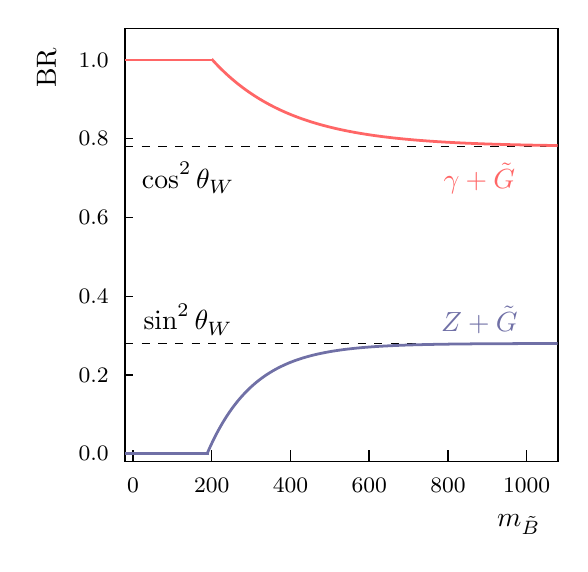
\begin{tikzpicture}

    \tikzstyle{region} = [rounded corners, fill, opacity=0.5, line width=0.1, green]
    \tikzstyle{axis} = [line width=0.6]
    \tikzstyle{tick} = [line width=0.5]
    \tikzstyle{point} = [blue, fill=blue!20]


    \draw[axis] (0,0) -- (5.5,0) node at (5.0,-0.8) {$m_{\tilde{B}}$};
    \draw[axis] (0,0) -- (0,5.5) node[rotate=90] at (-1,5.0) {BR};

    \draw[axis] (5.5,0) -- (5.5,5.5);
    \draw[axis] (0,5.5) -- (5.5,5.5);

    \draw[dashed] (0,1.5) -- (5.5,1.5) node[baseline=left] at (0.8, 1.8) {$\sin^2 \theta_W$};
    \draw[dashed] (0,4.0) -- (5.5,4.0) node[baseline=left] at (0.8, 3.6) {$\cos^2 \theta_W$};


    \draw[tick] (0,5.1) -- (0.1,5.1) node at (-0.4, 5.1) {\footnotesize 1.0};
    \draw[tick] (0,4.1) -- (0.1,4.1) node at (-0.4, 4.1) {\footnotesize 0.8};
    \draw[tick] (0,3.1) -- (0.1,3.1) node at (-0.4, 3.1) {\footnotesize 0.6};
    \draw[tick] (0,2.1) -- (0.1,2.1) node at (-0.4, 2.1) {\footnotesize 0.4};
    \draw[tick] (0,1.1) -- (0.1,1.1) node at (-0.4, 1.1) {\footnotesize 0.2};
    \draw[tick] (0,0.1) -- (0.1,0.1) node at (-0.4, 0.1) {\footnotesize 0.0};

    \draw[tick] (5.1,0) -- (5.1,0.15) node at (5.1,-0.3) {\footnotesize 1000};
    \draw[tick] (4.1,0) -- (4.1,0.15) node at (4.1,-0.3) {\footnotesize 800};
    \draw[tick] (3.1,0) -- (3.1,0.15) node at (3.1,-0.3) {\footnotesize 600};
    \draw[tick] (2.1,0) -- (2.1,0.15) node at (2.1,-0.3) {\footnotesize 400};
    \draw[tick] (1.1,0) -- (1.1,0.15) node at (1.1,-0.3) {\footnotesize 200};
    \draw[tick] (0.1,0) -- (0.1,0.15) node at (0.1,-0.3) {\footnotesize 0};

    \draw[blue, line width=1] (0,0.1) -- (1.06,0.1);
    \draw[blue,line width=1] plot[domain=1.04:5.5, samples=500] ({\x},{1.5*(1 - exp(-((\x-1)/0.6)))});

    \draw[red, line width=1] (0,5.1) -- (1.1,5.1);
    \draw[red,line width=1] plot[domain=1.1:5.5, samples=500] ({\x},{4.+1.5*(exp(-((\x-0.8)/1)))});

    \node[blue] at (4.5, 1.8) {$Z+ \tilde{G}$};
    \node[red]  at (4.5, 3.6) {$\gamma + \tilde{G}$};
\end{tikzpicture}

  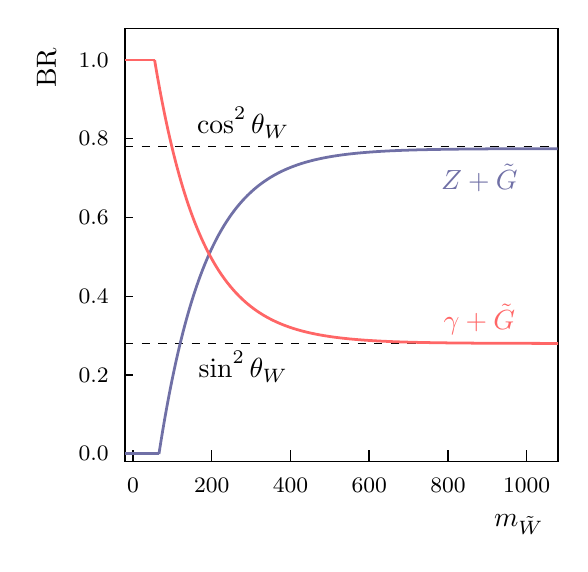
\begin{tikzpicture}

    \tikzstyle{region} = [rounded corners, fill, opacity=0.5, line width=0.1, green]
    \tikzstyle{axis} = [line width=0.6]
    \tikzstyle{tick} = [line width=0.5]
    \tikzstyle{point} = [blue, fill=blue!20]

    \draw[axis] (0,0) -- (5.5,0) node at (5.0,-0.8) {$m_{\tilde{W}}$};
    \draw[axis] (0,0) -- (0,5.5) node[rotate=90] at (-1,5.0) {BR};

    \draw[axis] (5.5,0) -- (5.5,5.5);
    \draw[axis] (0,5.5) -- (5.5,5.5);

    \draw[dashed] (0,1.5) -- (5.5,1.5) node[baseline=left] at (1.5, 1.2) {$\sin^2 \theta_W$};
    \draw[dashed] (0,4.0) -- (5.5,4.0) node[baseline=left] at (1.5, 4.3) {$\cos^2 \theta_W$};


    \draw[tick] (0,5.1) -- (0.1,5.1) node at (-0.4, 5.1) {\footnotesize 1.0};
    \draw[tick] (0,4.1) -- (0.1,4.1) node at (-0.4, 4.1) {\footnotesize 0.8};
    \draw[tick] (0,3.1) -- (0.1,3.1) node at (-0.4, 3.1) {\footnotesize 0.6};
    \draw[tick] (0,2.1) -- (0.1,2.1) node at (-0.4, 2.1) {\footnotesize 0.4};
    \draw[tick] (0,1.1) -- (0.1,1.1) node at (-0.4, 1.1) {\footnotesize 0.2};
    \draw[tick] (0,0.1) -- (0.1,0.1) node at (-0.4, 0.1) {\footnotesize 0.0};

    \draw[tick] (5.1,0) -- (5.1,0.15) node at (5.1,-0.3) {\footnotesize 1000};
    \draw[tick] (4.1,0) -- (4.1,0.15) node at (4.1,-0.3) {\footnotesize 800};
    \draw[tick] (3.1,0) -- (3.1,0.15) node at (3.1,-0.3) {\footnotesize 600};
    \draw[tick] (2.1,0) -- (2.1,0.15) node at (2.1,-0.3) {\footnotesize 400};
    \draw[tick] (1.1,0) -- (1.1,0.15) node at (1.1,-0.3) {\footnotesize 200};
    \draw[tick] (0.1,0) -- (0.1,0.15) node at (0.1,-0.3) {\footnotesize 0};

    \draw[blue, line width=1] (0,0.1) -- (0.43,0.1);
    \draw[blue,line width=1] plot[domain=0.43:5.5, samples=500] ({\x},{1.5*(2.65 - exp(-((\x-1)/0.6)))});

    \draw[red, line width=1] (0,5.1) -- (0.38,5.1);
    \draw[red,line width=1] plot[domain=0.375:5.5, samples=500] ({\x},{1.5+1.5*(exp(-((\x-0.9)/0.6)))});

    \node[blue] at (4.5, 3.6) {$Z+ \tilde{G}$};
    \node[red]  at (4.5, 1.8) {$\gamma + \tilde{G}$};
\end{tikzpicture}


  \caption{Tasas de decaimiento del neutralino más liviano a gravitino más fotones o bosones $Z$ en funcion de la masa del mismo. En la izquierda
    el caso que el neutralino es puramente bino, y a la derecha puramente wino.}
  \label{fig:bino_wino_br}
\end{figure}

Cuando la NLSP es mayormente wino, hay una muy pequeña degeneración entre el
wino neutro y el cargado. Cuando esto pasa, el decaimiento de tres cuerpos al
wino neutro comienza a ser excluido, y el wino cargado prefiere decaer
directamente a $W^{\pm}$ y un gravitino. En otras palabras, el wino neutro y el
wino cargado se vuelve co-NLSPs, y los estados finales van a contener $W$'s,
$Z$'s y fotones.

Como en cada evento de SUSY hay un par de neutralinos, los estados
finales involucrarán una combinación de pares de $\gam + \gravino$, $Z +
\gravino$ y $h + \gravino$. Adicionalmente, si hay una diferencia chica entre la masa
del neutralino y del chargino más liviano, puede haber cadenas de decaimiento
que terminen en $W^\pm + \gravino$.

El escenario más estudiado y más buscado es cuando la NLSP es un neutralino
puramente bino. En este caso el estado final consiste en $\gam\gam + \met$.
Sin embargo en el caso más general de neutralino NLSP, aparecen muchas otros
canales menos explorados que involucran leptones, $Z$, $W$, jets y higgses de
alto {\pt} y energía faltante.

%% Por otro lado, la degeneración\'on entre los higgsinos cargados y
%% neutros es generalmente mayor, de modo que solo el neutralino mas
%% livinao decae directamente en gravitino.

En el caso en el cual el neutralino es una mezcla mayoritaria de bino y higgsino, el
estado final dependerá del parámetro de masa del higgsino $\mu$. Si
$\mu <0$, el estado final de la cascada va a tener una gran contribución
de $\ninoone \to h\gravino$ donde el Higgs decaerá mayormente a $h\to b \bar{b}$,
dejando un estado final con un fotón, b-jets y {\met}. En el escenario donde
$\mu>0$ el decaimiento dominante estará compartido entre $\ninoone \to \gam\gravino$
y $\ninoone\to Z \gravino$, y el decaimiento a Higgs estara suprimido,
dando como estado final un fotón, múltiples jets (incluyendo
los dos del decaimiento de $Z$) y {\met}.

Esta Tesis se centrará en este ultimo caso. En el \cref{cap:simulaciones}
se describirá en detalle el modelo de se\~nal que motiva el estado final
de el presente análisis.


%% Esta Tesis se centrara en un neutralino NLSP que es una mezcla mayoritaria
%% de bino y higgsino, donde la probabilidad de decaimiento en fotones y $Z$
%% es similar y esta suprimido el decaimiento a Higgs, dejando como estado
%% final un único fotón, jets, y energía faltante.


\subsection{Producción de partículas supersimétricas}

En la \cref{fig:xs_lhc_8tev} se puede ver la sección eficaz para la producción
de squarks y gluinos en el LHC comparada para los distintos canales de
producción. La producción por interacción fuerte es mucho mayor a la de
spartículas que interactúan débilmente, y por esta razón la mayoría de las
búsquedas se basan en la producción de gluinos y squarks.

\begin{figure}[!htbp]
  \centering
  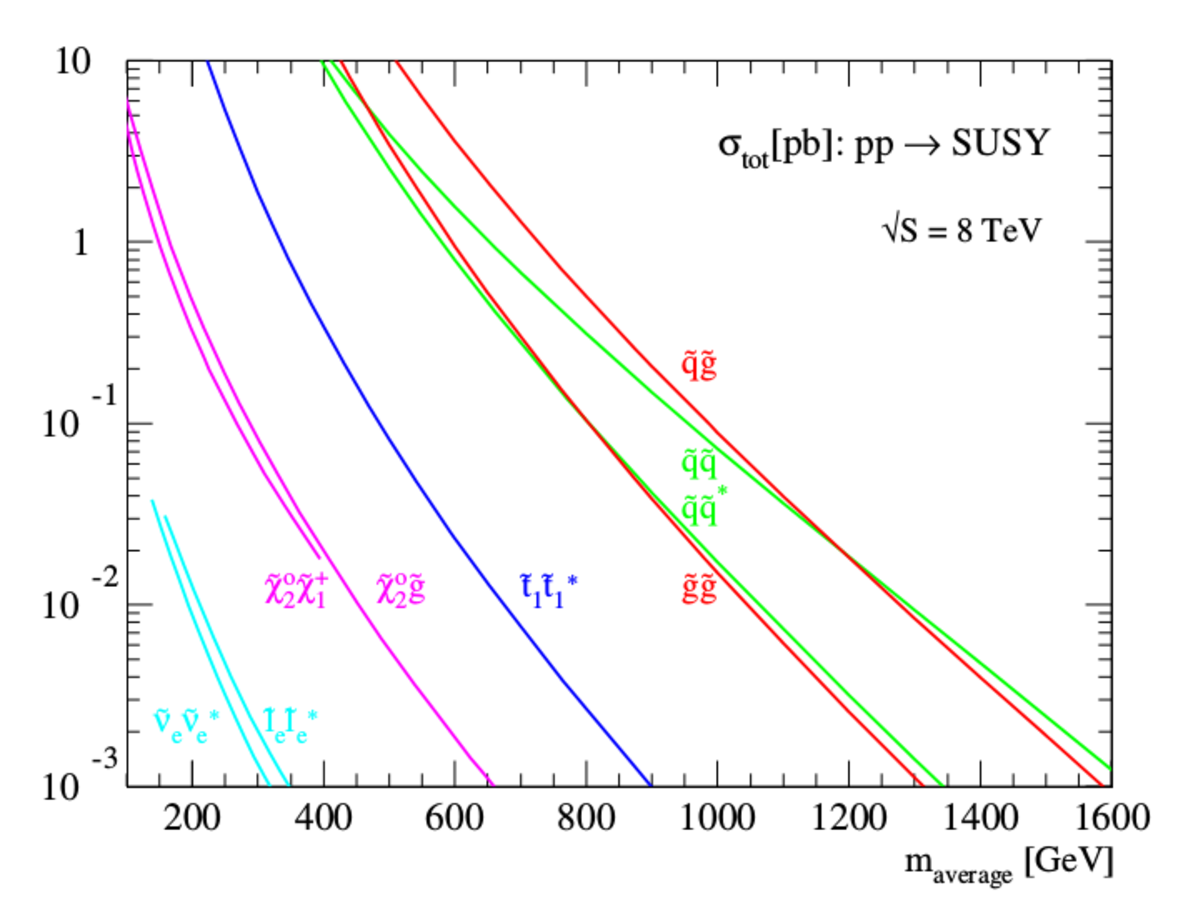
\includegraphics[width=0.8\textwidth]{figures/susy_lhc_xs_8tev}
  \caption{Sección eficaz de producción de partículas supersimétricas, como
    función de su masa, para los distintos canales de producción en el LHC con
    $\sqrt{s} = 8 \tev$ calculada a NLO usando \prospino.}
  \label{fig:xs_lhc_8tev}
\end{figure}


En los colisionadores hadrónicos, las partículas supersimétricas pueden ser
producidas de a pares a partir de colisiones de interacción
electrodébil (ver \cref{fig:ewkprod}):

\begin{align}
  &q\bar{q} \quad \to \quad \chinop \chinom, \nino \nino \label{eq:qq_ewk} \\
  &q\bar{q} \quad \to \quad \susy{\ell}^{+}_{i}\susy{\ell}^{-}_{j}, \susy{\nu}_{\ell}\susy{\nu}^{*}_{\ell} \label{eq:qq_ewk2}
\end{align}
%
y a partir de interacciones fuertes (ver \cref{fig:strongprod1,fig:strongprod2}):

\begin{align}
  gg \quad &\to \quad \gluino\gluino, \susy{q_i}\susy{q_j}^{*}, \label{eq:gg} \\
  gq \quad &\to \quad \gluino\susy{q_i}, \label{eq:gq} \\
  q\bar{q} \quad &\to \quad \gluino\gluino, \susy{q_i}\susy{q_j}^{*}, \label{eq:qqbar} \\
  qq \quad &\to \quad \susy{q_i}\susy{q_j}, \label{eq:qq}
\end{align}

La producciones en \cref{eq:qq_ewk,eq:qq_ewk2} obtienen contribuciones de los
bosones vectoriales electrodébiles en el canal $s$, mientras que las de
\cref{eq:qq_ewk} también tienen contribuciones del canal $t$ que son menos
importantes en la mayoría de los modelos. Los procesos en
\cref{eq:gg,eq:gq,eq:qqbar,eq:qq} tienen contribuciones del intercambio del
correspondiente squark o gluino en el canal $t$, y \cref{eq:gg} y
\cref{eq:qqbar} también tienen contribuciones de gluones en el canal $s$.

\begin{figure}[!htbp]
  \centering 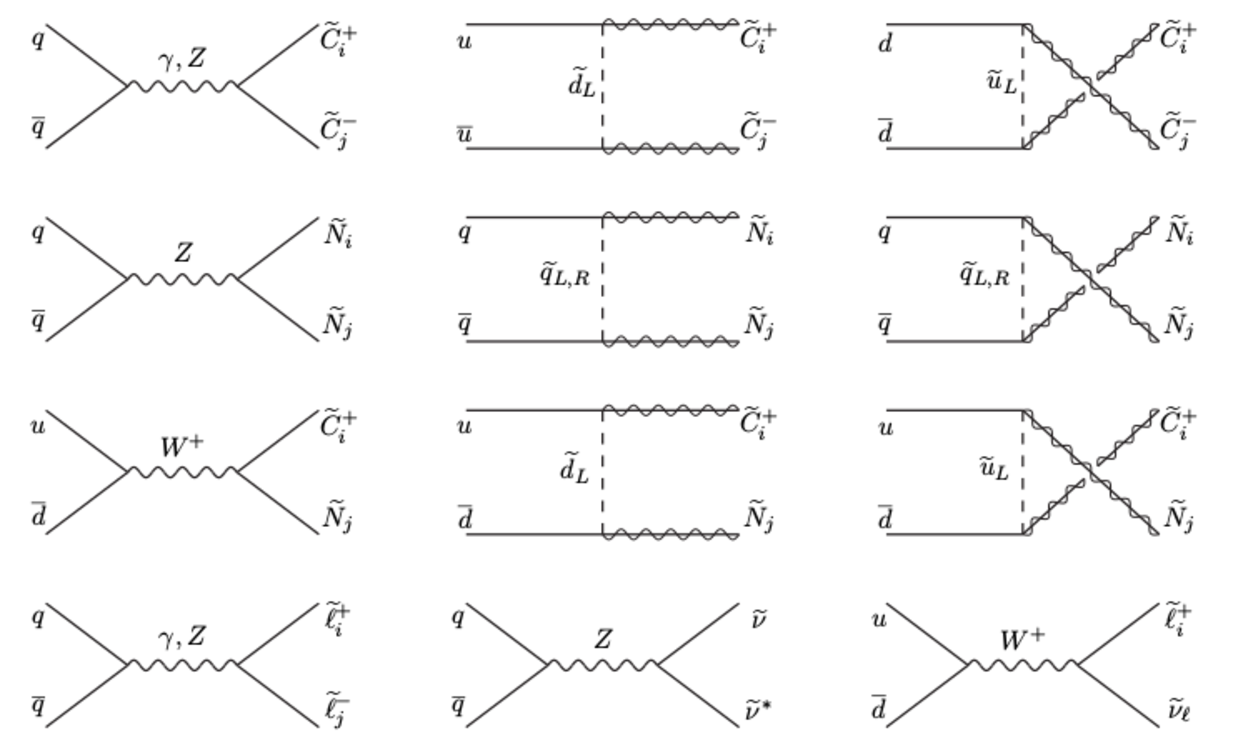
\includegraphics[width=0.6\textwidth]{figures/figure_101}
  \caption{Diagramas de Feynman para la producción electrodébil de spartículas
    en colisionadores de hadrones vía aniquilación quark-antiquark.}
  \label{fig:ewkprod}
\end{figure}

\begin{figure}[!htbp]
  \centering 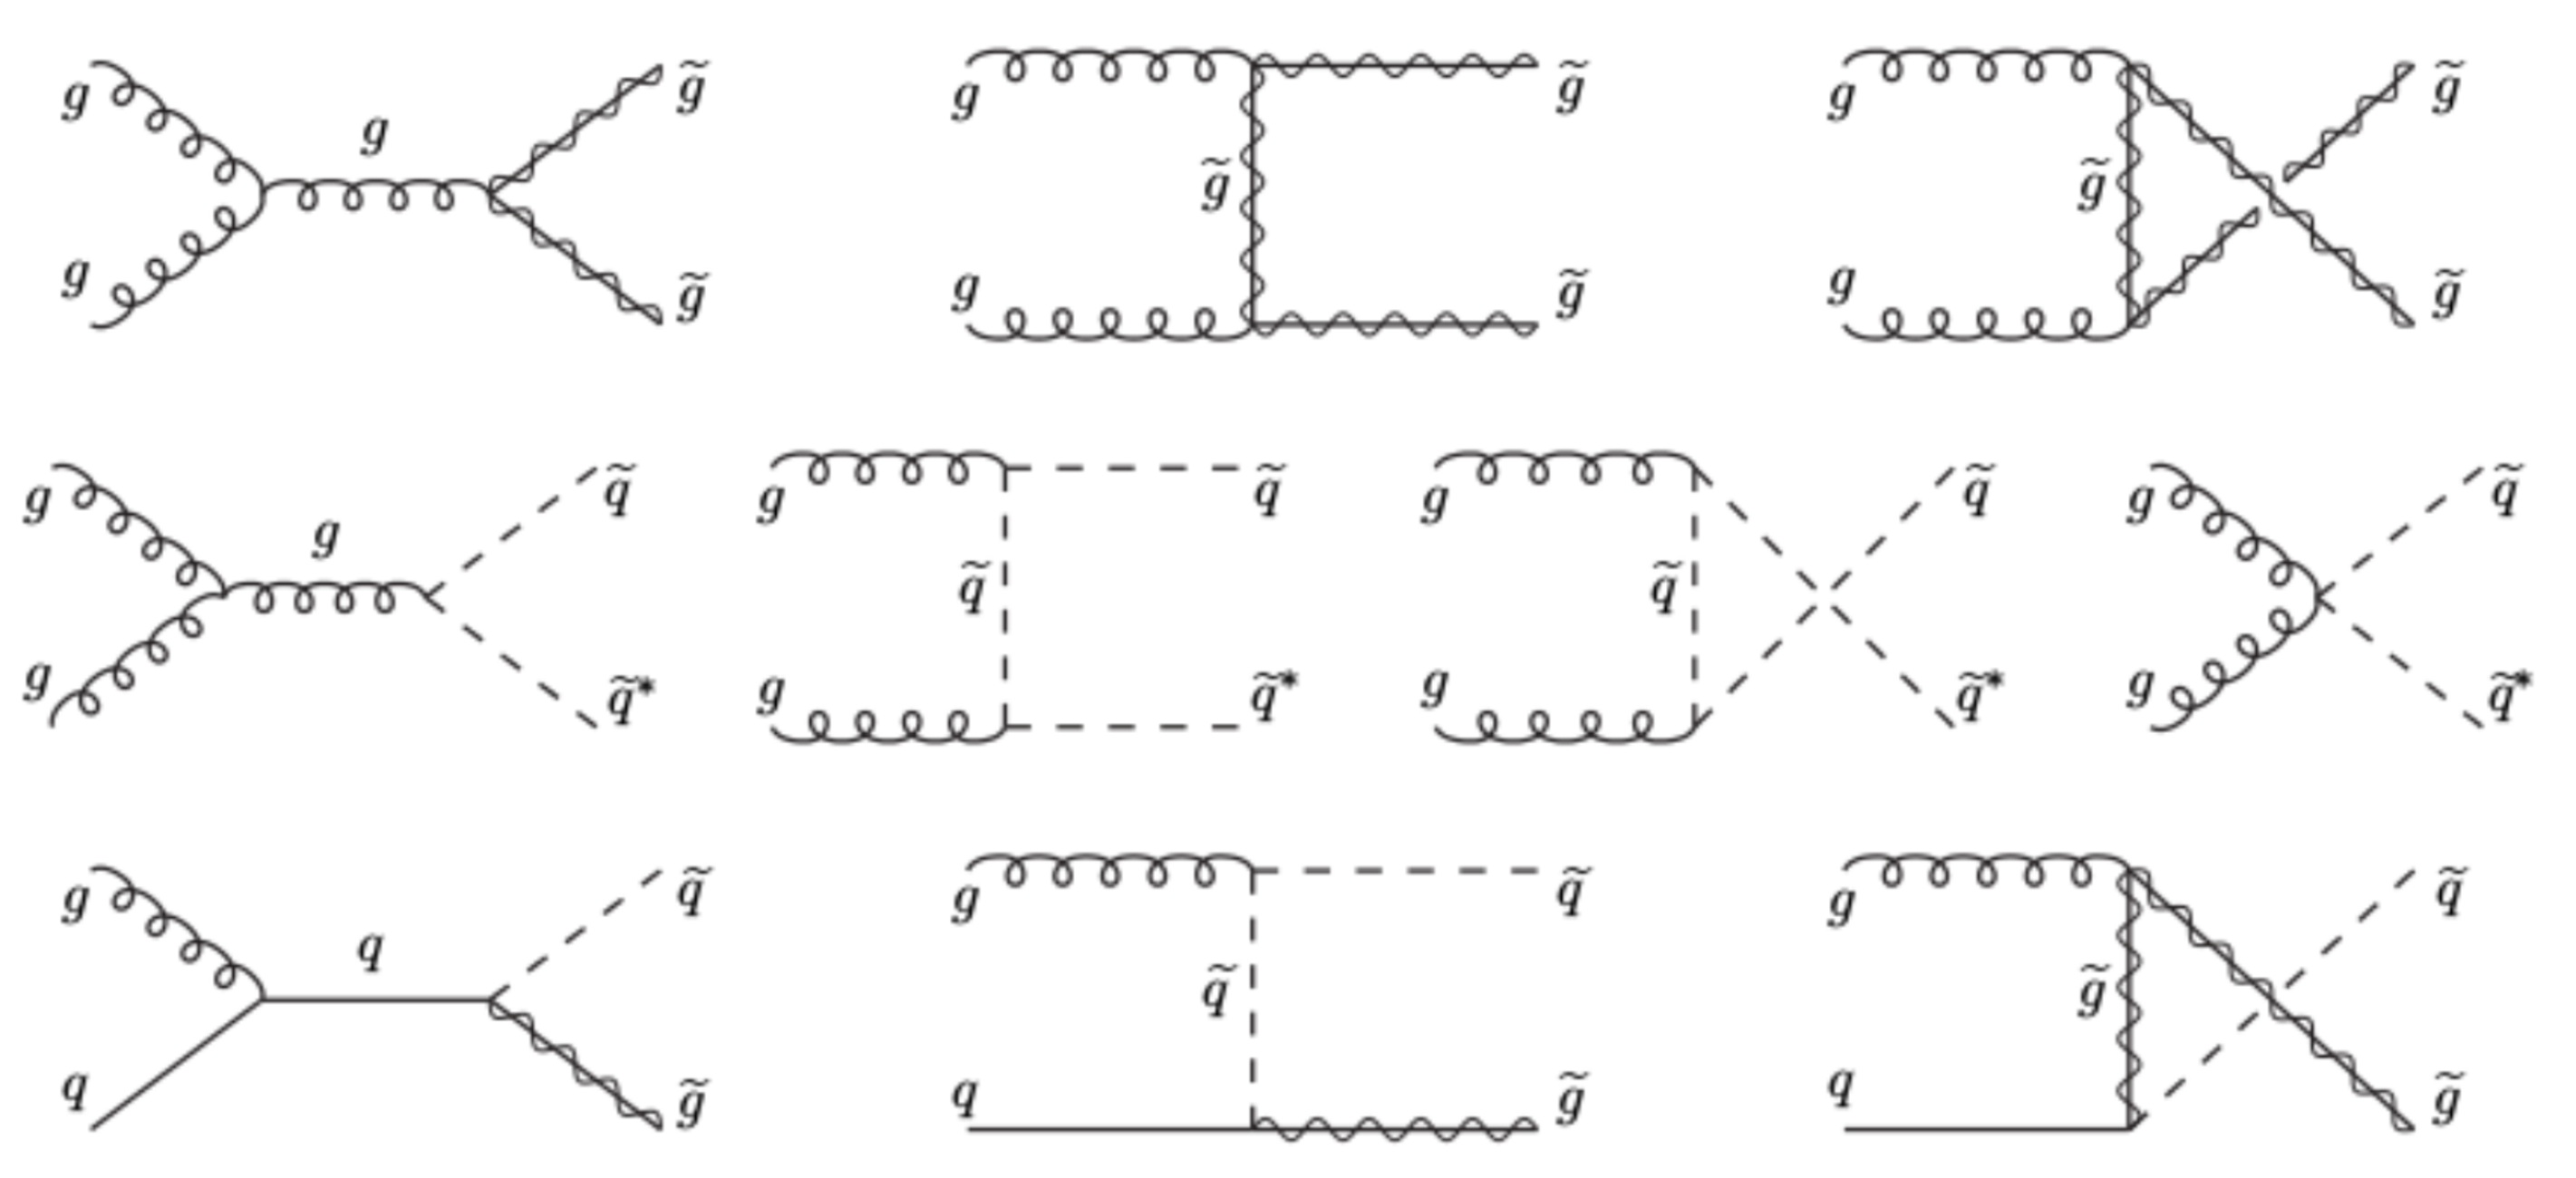
\includegraphics[width=0.6\textwidth]{figures/figure_102}
  \caption{Diagramas de Feynman para la producción de gluinos y squarks en
    colisionadores de hadrones vía fusión gluón-gluón y gluón squark.}
  \label{fig:strongprod1}
\end{figure}

\begin{figure}[!htbp]
  \centering 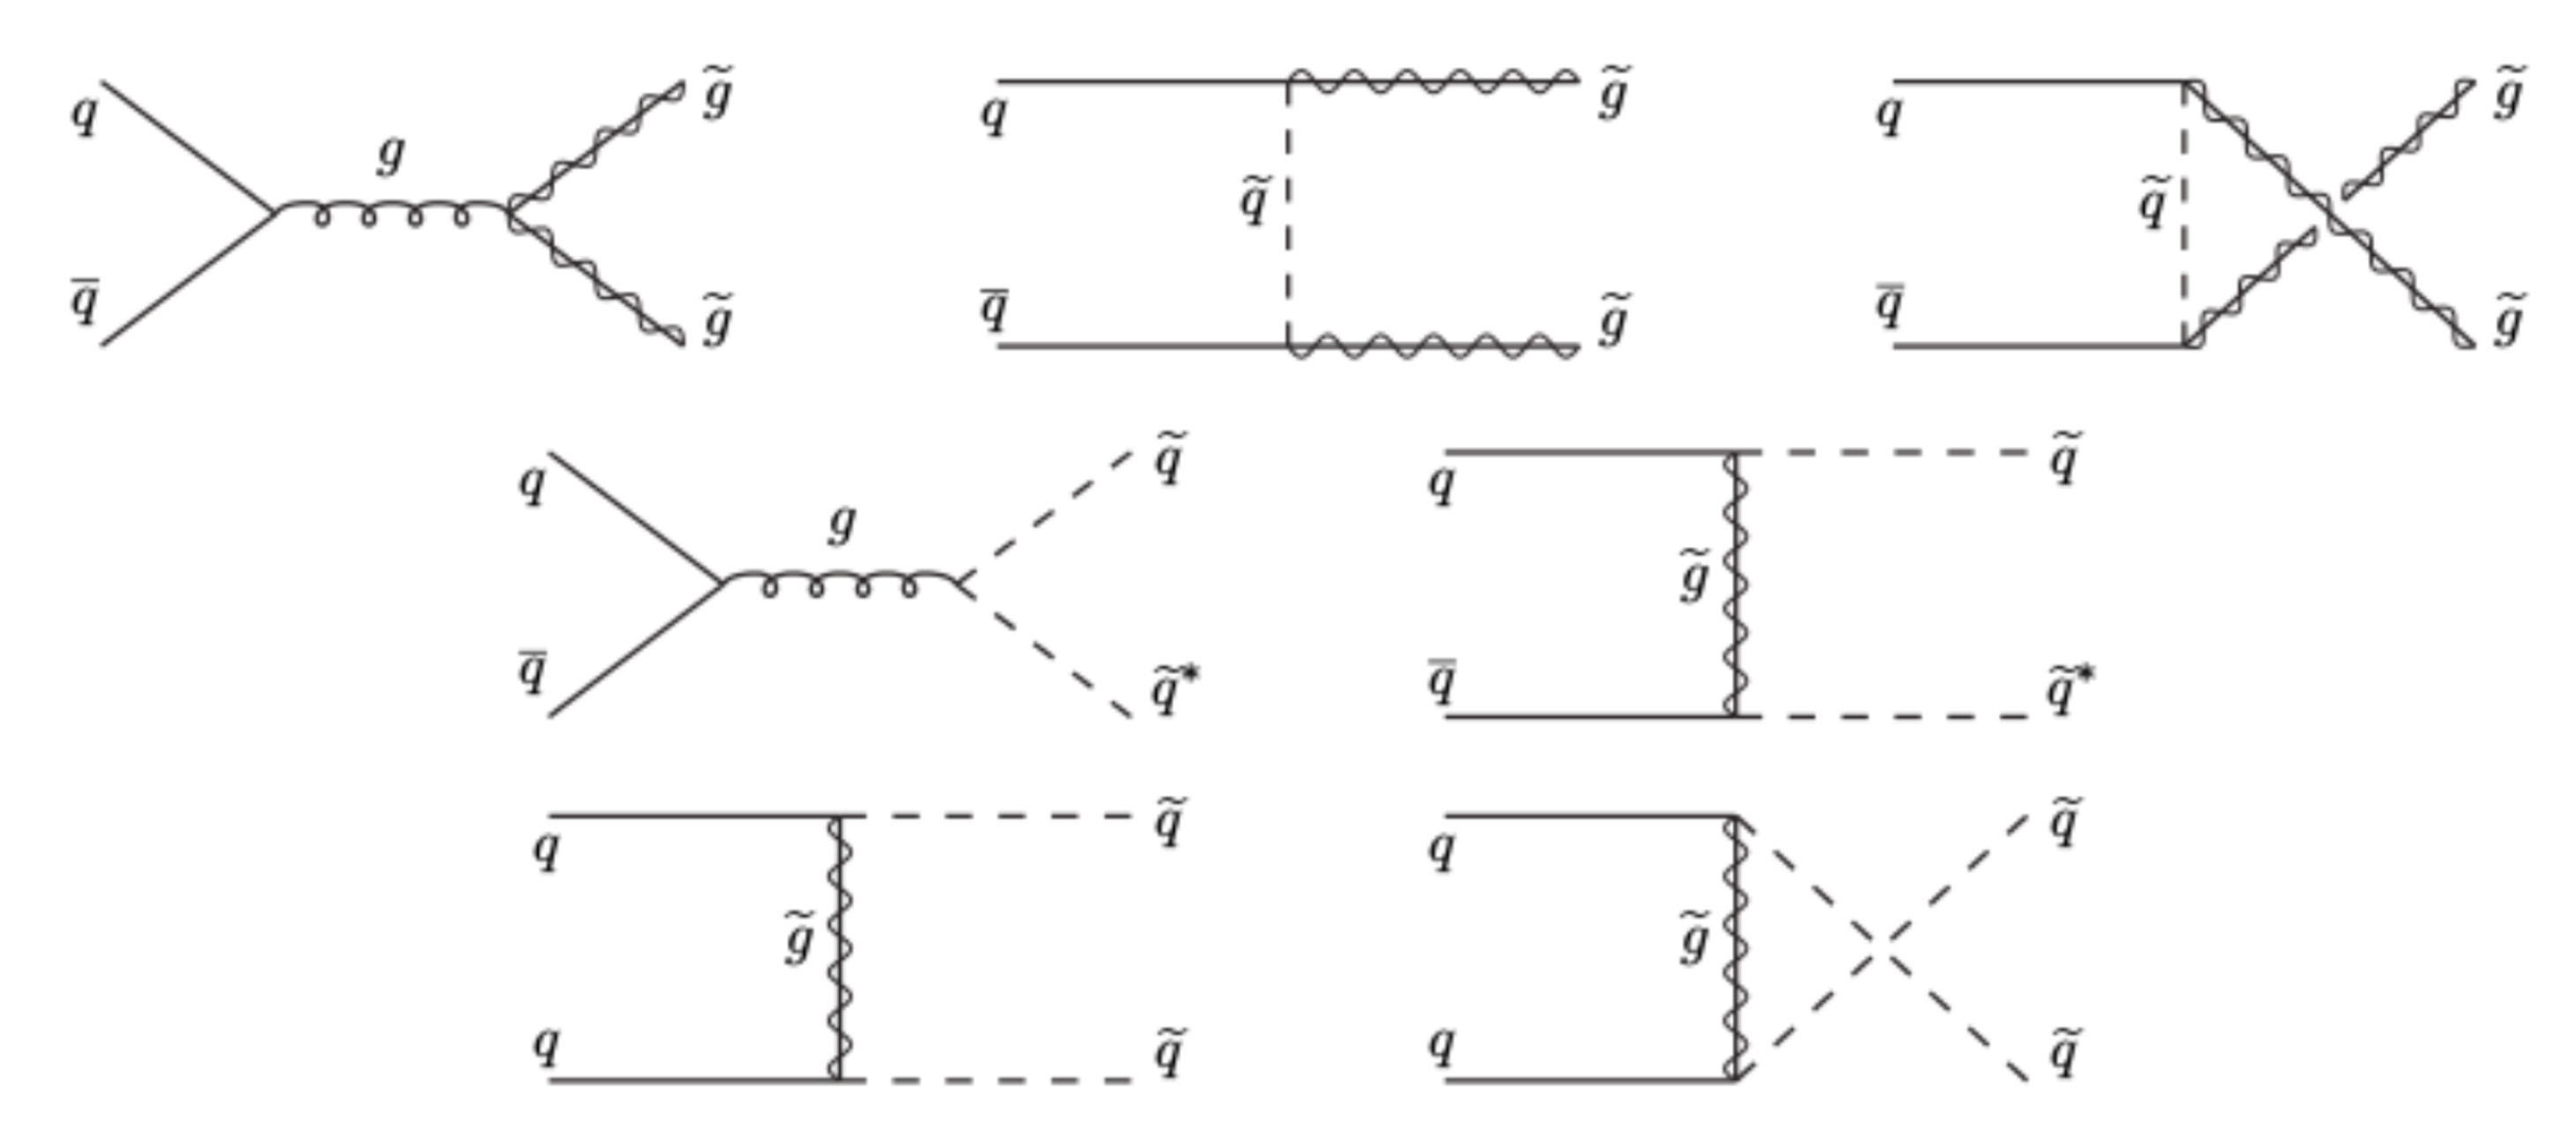
\includegraphics[width=0.6\textwidth]{figures/figure_103}
  \caption{Diagramas de Feynman para la producción de gluinos y squarks en
    colisionadores de hadrones vía aniquilación quark-antiquark y dispersión
    quark-quark}
  \label{fig:strongprod2}
\end{figure}


%% En Tevatron, los procesos de produccion de charginos y neutralinos tienden a tener
%% mayores seccion eficaz, a menos los squarks o el gluino sean muy liviano (menos a 300 \gev,
%% masas que ya se encuentran excluidas por el LHC). En el LHC, la situacion es opuesta, con la
%% produccion de gluinos y squarks dominante por medio de gluon-gluon y gluon-quark fusion.
%% En ambos colisionadores, puede haber produccion asociada de chargino o neutralino junto con
%% un squark y un gluino, pero la mayoria de los modelos predicen que la seccion eficaz


%%\part{Experimento}
\chapter{LHC y el detector ATLAS}


\section{LHC}

El Gran Colisionador de Hadrones (LHC, del ingles Large Hadron Collider) es el acelerador
de hadrones ubicado en el laboratorio CERN\footnote{CERN son las siglas en francés de
  \emph{Conseil Européen pour la Recherche Nucléaire}}, en la frontera entre Francia y Suiza.
Posee una longitud de 27 km y fue construido en el mismo túnel en el que funcionaba el acelerador
de electrones LEP entre 1989 y el 2000.

El LHC está diseñado para acelerar protones a 7 \tev, alcanzando energías de centro de masa de 14 \tev,
y una luminosidad de $10^{34}$ cm$^{-2}$s$^{-1}$.
Uno de los parámetros mas importantes para caracterizar el funcionamiento del acelerador es la
luminosidad instantánea (L), definida como el numero de partículas por unidad de tiempo por unidad de
área, que puede calcularse mediante la relación:

\begin{equation}
  L = f_\text{rev} n_b \frac{N_1 N_2}{A}
\end{equation}
%
donde $f$ es la frecuencia de revolucion (sim 11 kHz), $n_b$ es el numero de \emph{bunches}
(paquetes de protones) por haz, $N_i$ es el numero de partículas en cada bunch y A es la
sección efectiva del haz, que puede expresarse en termino de los parámetros del acelerador
como:

\begin{equation}
  A = \frac{4\pi \epsilon_n \beta^{*}}{\gamma F}
\end{equation}
%
donde $\epsilon_n$ es la emitancia transversal normalizada (la dispersión transversal media de las
partículas del haz en el espacio de coordenadas e impulsos), $\beta^{*}$ es la función de amplitud
en el punto de interacción (IP), relacionada al poder de focalización de los cuadrupolos), $\gamma$
es el factor relativista de Lorentz y $F$ es un factor de reducción geométrico, debido al ángulo
de cruce de los haces en el IP.


Durante el año 2010, las colisiones se realizaron a 3.5 TeV por haz (7 TeV de energía de centro de masa)
y con una luminosidad que fue incrementándose hasta alcanzar los $2 \times 10^{32}$ cm$^{-2}$ s$^{-1}$
en Octubre. %%\todo{complete with 8 TeV run}

El diseño contempla trenes de 2808 paquetes de $\sim 10^{11}$ protones cada uno,
espaciados temporalmente en 25 ns.

Para acelerar los haces de protones y mantenerlos en sus orbitas circulares el LHC cuenta con 1232
dipolos magnéticos superconductores que generan un campo magnético de 8.4 T enfriados a 1.9 K.
El sistema de focalización de los haces consiste de 392 cuadrupolos magnéticos que generan campos
magnéticos de 6.8 T. Los haces circulan en direcciones opuestas en cavidades de ultra alto vacío
separadas a presión de 10$^{-10}$ torr.


\section{ATLAS}

ATLAS es un detector de partículas multipropósito del LHC diseñado y construido para estudiar
las colisiones protón-protón a una energía de centro de masa de hasta 14 TeV.
El nombre significa \textbf{A T}orodial \textbf{L}HC aparatu\textbf{S}.

%% Los criterios básicos para el diseño del detector de ATLAS fueron:

%% \begin{itemize}
%% \item Un muy buen calorímetro electromagnético para la identificación y medidas de fotones y electrones, complementado con un calorímetro hadrónico para las medidas precisas de \emph{jets} y energía transversa perdida.
%% \item Medidas de alta precisión de momentos de muones, con la capacidad de garantizar mediciones precisas a la mas alta luminosidad usando sólo el espectrómetro de muones externo.
%% \item Alta eficiencia de la detección de trazas a alta luminosidad para medidas de momentos de leptones con alto \pt, identificación de electrones y fotones, identificación de $\tau$,  y capacidad de reconstrucción total de eventos con luminosidad baja.
%% \item Gran aceptancia en pseudorapidez ($\eta$) cubriendo casi todo el ángulo azimutal ($\phi$) en todo el detector.
%% \item Selección y medidas de partículas con bajo \pt, proveyendo alta eficiencia para la mayor parte de los procesos físicos de interés en el LHC.
%% \end{itemize}


El esquema general del detector se muestra en la figura \ref{fig:atlas}, donde se señalan los
componentes principales.
ATLAS está diseñado en capas de subdetectores que cumplen diferentes roles en la identificación
de las partículas producidas en las colisiones pp del LHC.
Desde el punto de colision hacia afuera ATLAS se compone de un ID subdividido a su vez en un
detector de píxeles (o capa B), un detector de bandas de silicio (SCT) y un detector de radiación
de transición (TRT).

\begin{figure}[H]
  \centering
  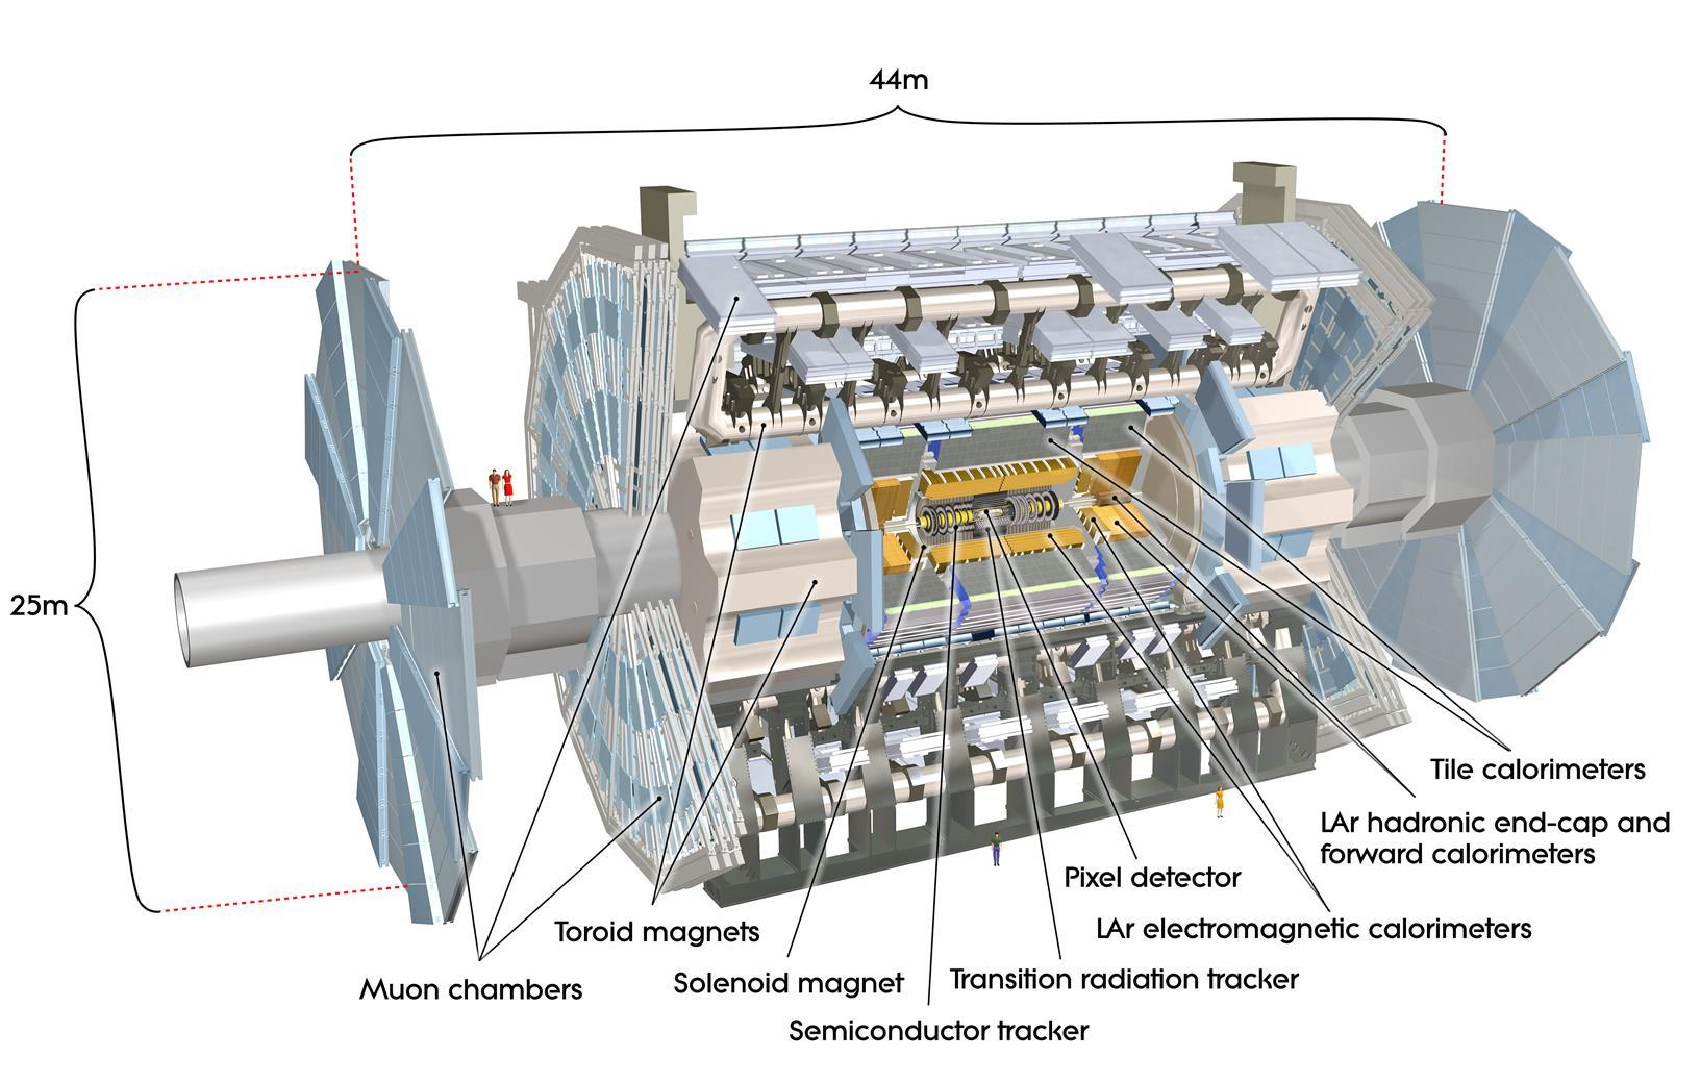
\includegraphics[width=0.85\textwidth]{figures/atlas}
  \caption{Esquema general del detector de ATLAS}\label{fig:atlas}
\end{figure}


Envolviendo este detector interno se encuentra un solenoide superconductor que genera un campo
magnético de $\sim$2 Tesla para que las partículas cargadas curven su trayectoria.
A continuación están ubicados los calorímetros: el calorímetro electromagnético para medir la
energía cinética de electrones y fotones, y posteriormente el calorímetro hadrónico para medir
la energía de los \emph{jets} de hadrones.

En la capa más externa se encuentra el espectrómetro de muones que le da a ATLAS el tamaño total
de aproximadamente 45m de largo y más de 25m de alto.
Intercalado con éste se encuentra el sistema de toroides que genera el campo magnético de $\sim$4
Tesla para curvar la trayectoria de los muones hacia el final de su pasaje por el detector ATLAS.

El detector ATLAS se divide geométricamente en dos regiones, la región del barril
(la parte central, \emph{barrel}) y la región de las tapas (ambos extremos, \emph{end-cap}).
En cada una de estas regiones la ubicación de los subdetectores es distinta. En la región del barril,
los subdetectores están ubicadas como cilindros concéntricos, mientras que en la región de las tapas
están ubicados como discos consecutivos.

\subsection{Sistema de coordenadas}

El sistema de coordenadas de ATLAS corresponde a un sistema cartesiano, cuyo origen
coincide con el punto de interacción nominal. El eje z es escogido, naturalmente dada la
concepción cilíndrica del detector, a lo largo del eje del haz, en sentido antihorario. El eje
$z$ positivo (negativo) define el lado A (C) del detector, en vista de la simetría nominal del

mismo. El plano transversal $x-y$ es definido con valores positivos de $x$ e $y$ desde el origen
en dirección hacia el centro del anillo del LHC y hacia la superficie, respectivamente.
Para describir la posición de los distintos subdetectores y la trayectoria de las partículas
dentro de ATLAS se utilizan frecuentemente sistemas de coordenadas cilíndricas o polares.
El radio R se define como la distancia perpendicular al eje del haz.  El ángulo azimutal
$\phi = 0$ corresponde al eje $x$ positivo y crece en sentido horario entorno al eje $z$ positivo,
mientras que el angulo $\theta$ se mide con respecto a este ultimo. Una cantidad muy importante
utilizada en física de altas energías es la llamada rapidez:

\begin{equation}
  y = \frac{1}{2} \ln \left( \frac{E+p_z}{E-p_z} \right)
\end{equation}
%
donde E es la energia total de la particula y $p_z$ es la componente longitudinal de su impulso.
En el limite de altas energias esta cantidad se aproxima (en forma exacta para objetos no masivos)
por la llamada \emph{pseudorapidez}, $\eta$, relacionada con el angulo polar $\theta$ como:

\begin{equation}
  \eta = - \ln \tan \left( \frac{\theta}{2} \right)
\end{equation}

La razon detras de esta transformacion de coordenadas es el hecho que la multiplicidad de particulas
producidas es aproximadamente constante como funcion de $\eta$, y que la
diferencia de pseudorapidez entre dos particulas es invariante frente a transformaciones
(boosts) de Lorentz a lo largo de la direccion del haz. En el caso de colisiones hadronicas,
la fraccion del impulso del proton adquirida por cada uno de las partones interactuantes
es desconocida; parte de este impulso es transferido en la interaccion dura, mientras cierta
fraccion remanente escapa el detector a lo largo del haz. Asi, no es posible reconstruir el
movimiento longitudinal del centro de masa en la interaccion, y aplicar leyes de conservacion
sobre la cinematica de cada evento. Sin embargo, dado que los protones inciden a lo
largo de la direccion del haz, el impulso total transverso es conservado durante la colision.
Por esta razon, solo las componentes transversales son utilizadas en la descripcion de la
cinematica del evento, e.g. $\et (= E \sin \theta)$ y $\pt (= p \sin \theta)$.
En terminos de la pseudorapidez, la energia transversa de una particula resulta:


\begin{equation}
  \et = \frac{E}{\cosh \eta}
\end{equation}
%
donde $E$ es su energia total.


\section{Los subdetectores de ATLAS}

A continuacion se describen brevemente cada uno de los subdetectores, particularmente
aquellos subsistemas utilizados para la identificacion de electrones y fotones, pertinentes
al analisis presentado en esta tesis.

\subsection{El detector interno}

El esquema del detector interno se muestra en la figura \ref{fig:innerdetector}\cite{IDTDR}.
Este sistema combina detectores de muy alta resolución para distancias cortas al punto de interacción con detectores continuos de trazas a distancias más lejanas. El detector interno está contenido dentro del solenoide que provee un campo magnético nominal de 2T.

\begin{figure}[H]
  \centering
  \includegraphics[width=0.55\textwidth]{figures/figura}
  \caption{Esquema del detector interno}\label{fig:innerdetector}
\end{figure}

\subsubsection{Pixel}
Más cerca del punto de interacción se encuentra el detector de píxeles que se compone de tres capas en el barril (a 4cm, a 10cm y a 13 cm del tubo del haz de protones) y tres discos en cada tapa.  Proveen mediciones de altísima precisión y granularidad tan cerca del punto de interacción como es posible. El sistema contiene en total 80 millones de elementos de 14x115 $\mu$m en (R$\phi$,z), capaces de resolver la posición de las partículas mejor que 14$\mu$m.

\subsubsection{SCT}
Por fuera del detector de píxeles se encuentra el detector semiconductor de trazas (SCT) que consta de ocho capas de detectores de micro bandas de silicio que provee puntos de alta precisión en las coordenadas (R$\phi$,z).
La resolución espacial es de 16 $\mu$m en R$\phi$ y de 580 $\mu$m en z y tiene 6.2 millones de canales.
Las trazas pueden distinguirse si están separadas más de $\sim$200 $ \mu$m.
El SCT cubre el rango de pseudorapidez de $|\eta|<$2.5.


\subsubsection{TRT}
La parte más externa del detector de trazas es el detector de radiación de transición (TRT).
Este detector está basado en el uso de detectores tubos que pueden operar a alta frecuencia de eventos gracias a su pequeño diámetro (4mm) y la aislación de sus hilos centrales en volúmenes de gas individuales.

El TRT además de detectar el pasaje de partículas cargadas, detecta la radiación de transición que permite distinguir entre partículas cargadas pesadas y livianas.
La separación entre señales de trazas y de radiación por transición se hace analizando tubo por tubo impactos de alto umbral e impactos de baja señal.
El largo de los tubos varía segun la zona del detector, llegando hasta los 144 cm en la zona del barril.
El Barril contiene 50000 tubos y las tapas contienen 320000 tubos orientados radialmente. El número total de canales es de 420000 y la resolución espacial es de 0.17mm.


\subsection{Calorímetros}

Una vista de los calorímetros de ATLAS puede verse en la figura \ref{fig:calo}. Consiste en un calorímetro electromagnético cubriendo la región de pseudorapidez $|\eta| < 3.2$, un calorímetro hadrónico en la sección \emph{barrel} cubriendo la región $|\eta| < 3.2$, calorímetro hadrónicos en las \emph{end-cap} cubriendo la región $1.5 < |\eta| < 3.2$, y calorímetros \emph{forward} cubriendo $3.1 < |\eta| < 4.9$.

\begin{figure}[H]
  \centering
  \includegraphics[width=0.5\textwidth]{figures/figura}
  \caption{Esquema general del calorímetro del detector de ATLAS}\label{fig:calo}
\end{figure}


\subsubsection{Calorímetro electromagnético}
El calorímetro electromagnético \cite{caloemTDR} se divide en una parte central
(\emph{barrel}): $|\eta|<$1.475) y los extremos (\emph{end-caps}): 1.375$<|\eta|<$3.2.
El barril está compuesto por dos mitades, separadas por una distancia pequeña (6 mm) a $z = 0$.
Las tapas del calorímetro están divididas en dos ruedas coaxiales: una rueda
externa cubriendo la región 1.375$<|\eta|<$2.5 y una parte interna que cubre la
región 2.5$<|\eta|<$3.2.

El calorímetro electromagnético es un detector de muestreo de Argón Líquido (LAr)
con electrodos de kaptón en forma de acordeón y planchas absorbentes de plomo.
El espesor total del calorimetro electromagnetico\ es $>$24 $X_0$ en el barril
y $>$26 $X_0$ en las tapas, ($X_0$ = longitud de radiación).

En la región dedicada a los estudios de física de precisión ($|\eta|<$2.5) el
calorímetro electromagnético está segmentado en tres secciones longitudinales.% como se esquematiza en la figura \ref{fig:caloem}.

%\begin{figure}[H]
%  \centering
%  \includegraphics[width=0.85\textwidth]{./chapters/atlas/images/caloem}
%  \caption{Calorímetro Electromagnético del detector de ATLAS}\label{fig:caloem}
%\end{figure}


La sección de las bandas (\emph{strips}) que tiene un espesor constante de $\sim$6 $X_0$ en función de $\eta$, está equipado con bandas finas de 4 mm de largo en la dirección $\eta$.
Esta sección actúa como un detector de pre-cascada (\emph{pre-shower}) aumentando la capacidad de identificación de partículas, (como por ejemplo la distinción entre $\gamma$ y $\pi_0$ o entre electrón y $\pi^\pm$) y dando una precisa medición de la posición en $\eta$.

La sección del medio está segmentada transversalmente en torres cuadradas de $\Delta \phi \times \Delta \eta=$0.025 $\times$ 0.025 (4 $\times$ 4 cm$^2$ en $\eta=0$).
El espesor total del detector hasta el final de la sección del medio es $\sim$24$X_0$.

La sección mas externa tiene una granularidad de $\Delta\phi\times\Delta\eta=$0.025 $\times$ 0.05 y su espesor varía entre 2 y 12 $X_0$.

\subsubsection{Calorímetro hadrónico}
El calorímetro hadrónico de ATLAS \cite{calohadTDR} cubre el rango $|\eta|<$4.9 usando diferentes materiales.

La parte del barril de este sistema consiste en un calorímetro de muestreo que utiliza
acero como absorbente y tejas centelladoras como material activo.
Las tejas están ubicadas radialmente y apiladas en profundidad.

%\begin{figure}[H]
%  \centering
%  \includegraphics[width=0.85\textwidth]{./chapters/atlas/images/calohad}
% \caption{Calorímetro Hadrónico del detector de ATLAS}\label{fig:calohad}
% \end{figure}

La estructura es periódica en z. Las tejas tienen un espesor de 3 mm y el
espesor de las placas de acero en un período es de 14 mm.

El calorímetro de tejas se extiende radialmente desde un radio interno de 2.28 m
hasta un radio externo de 4.25 m.

En la región de las tapas, el calorímetro hadrónico consiste en dos ruedas de 2.3 m de
radio, perpendiculares al tubo del haz, hechas con placas de cobre y tungsteno como material
absorbente y argón líquido como material activo.
Estos detectores extienden la aceptancia del calorímetro de ATLAS hasta prácticamente
cubrir el ángulo sólido del punto de colisión.


\subsection{Espectrómetro de muones}
Los muones de alto {\pt} generados en el punto de interacción tienen un altísimo poder de
penetración y son poco interactuantes.
Por ello el espectrómetro de muones \cite{muonTDR} se encuentra situado en la parte más
exterior del detector ATLAS, alrededor del sistema de imanes de toroides,
y está diseñado para obtener mediciones de alta precisión de posición e impulso de muones de alto \pt.

\begin{figure}[H]
  \centering
  \includegraphics[width=0.7\textwidth]{figures/figura}
  \caption{Espectrómetro de muones del detector de ATLAS}\label{fig:especmuones}
\end{figure}

La figura \ref{fig:especmuones} muestra un esquema del espectrómetro de muones de ATLAS.
Es el subdetector más grande y el que le da a ATLAS su tamaño.

La región del barril está compuesta por tres capas concéntricas de cámaras de trigger
y de cámaras de precisión posicionadas a  5m, 7.5m y 10m del tubo del LHC, cubriendo
la región $|\eta|<1$.
Las regiones de las tapas están compuestas por cuatro capas de cámaras de trigger y
cámaras de precisión a $|z|$= 7.4m, 10.8m, 14m y 21.5m cubriendo el rango de 1.0$<|\eta|<$2.7.
Hay una pequeña brecha en $|z|=0$ que permite el acceso de los servicios al ID.

%---------
% Trigger
%---------
\section{El sistema de Trigger}

Bajo las condiciones nominales de dise\~no del LHC, la tasa de interaccion proton-proton
en el LHC sera de $\mathcal{O}(1)$ GHz, considerando una frecuencia de bunch crossing
de 40 MHz y $\sim$ 23 interacciones por cruce. Dado que la mayoria de los eventos son
de baja energia y no son de interes para los analisis mas relevantes en ATLAS, y tambien
debido a las limitaciones de almacenamiento y del poder de computo, el flujo de datos
incidente debe ser reducido al maximo permitido para su almacenamiento permanente
($\sim 200$ Hz). El tamano tipico por evento es de $\sim 1.4$ MB, lo que resulta en un
ancho de banda requerido de $\sim 300$ MB/$s$. Esta reduccion se logra mediante una rapida
y eficiente preseleccion de eventso, conocida como \emph{trigger}. El sistema de trigger
de ATLAS [ref] esta organizado en tres niveles jerarquicos: \emph{Nivel 1} (L1),
\emph{Nivel 2} (L2) y \emph{Filtro de eventos} (EF), dondoe los dos ultimos conforman
el \emph{High Level Trigger} (HLT). Cada nivel permite analizar los eventos con mayor detalle,
aumentando la precision de los criterios de seleccion y la complejidad
de los algortimos utilizados. El sistema de adquisicion de datos (DAQ) transfiere y almacena
los datos seleccionados por el trigger. La {\fig} {\XXX} muestra un esquema del sistema de
Trigger-DAQ de ATLAS.

El primer nivel del trigger se encarga de la seleccion inicial, reduciendo la frecuencia
de eventos que pasaran al siguiente nivel a $\sim 75$ kHz. Debido al tamano limitado
de las memorias temporales (buffers) donde se guardan los datos de cada subdetector y al
considerable tiempo de vuelo de las particulas hasta el espctrometro de muones, la decision
debe tomarse en una escala de tiempo muy limitada ($2.5 \mu s$). El nivel 1 esta basado
en hardware y selecciona objetso de alto {\pt} construidos a partir de la informacion
de varios subdetectores. Los muones son identificados en las camaras de trigger descriptas
en la sec XXX, mientras que la informacion de los calorimetros, con una resolucion reducida,
se utiliza para identificar candidatos a electrones, fotones, jets y taus decayendo
hadronicamente. La posicion de cada objeto encontrado define una \emph{region de interes}
(RoI) en un evento potencialmente interesante, que se extiende como un cono desde el punto de
interaccion a lo largo del detector.

En el calorímetro, el L1 se basa en las se\~nales analógicas obtenidas en cada trigger
tower (i.e. suma de celdas en una ventana $\Delta \eta \times \Delta \phi = 0.1 \times 0.1$),
definida separadamente para el ECAL y el HCAL (Fig. 3.7). El trigger de muones en el L1 utiliza las medidas de
las trayectorias en las diferentes estaciones de las cámaras de trigger: las RPCs en la región
del barrel y las TGCs en los endcaps. La aceptancia geométrica del L1 trigger esta a ligada
al dise\~no del detector, donde las medidas de precisión en los calorímetros y la cobertura
del detector interno están limitadas a la región $\abseta < 2.5$. El trigger de fotones, electrones,
muones y taus debe asegurar la cobertura en esta región. En el caso del trigger de jets,
las trigger towers se extienden hasta $\abseta < 3.2$, mientras que para el calculo de la energía
transversa total (perdida) se utiliza todo el sistema calorimétrico (i.e. $\abseta < 4.9$).
Los resultados de los subsistemas del trigger son procesados en el Central Trigger Processor
(CTP), en donde se aplica una serie de selecciones (\emph{menu}) definidas como una
combinación de criterios individuales, que pueden ser ajustados según la luminosidad y los
requerimientos físicos particulares de cada toma de datos. Un total de 256 configuraciones
(\emph{items}) estan disponibles en el L1, donde se programa el tipo de RoI (EM, TAU, JET, etc.)
y los umbrales de energía total y de aislamiento requeridos en cada caso. Por ejemplo,
el  item L1EM14 acepta eventos donde al menos un (dos) cluster(s) en el calorímetro
electromagnético posee(n) $\et \geq 14 \GeV$.

El segundo nivel del trigger (L2) se centra unicamente en las RoIs donde el L1
encontro actividad, combinando informacion de todos los subdetectores dentro de cada una
($\sim 2$ % de la cobertura total del detector). El L2 consiste de una serie de algoritmos de
reconstruccion y seleccion especializados, dise\~nados para reducir la frecuencia de
eventos hasta aproximadamente 1 kHz. Estos algoritmos estan implementados en clusters de
procesamiento dedicados (PC farms) que analizan cada evento dentro de un tiempo de
latencia medio de $\sim \unit[40]{ms}$. El menor flujo de informacion en este nivel del trigger permite
calcular las variables calorimetricas con mayor precision y hacer uso de la informacion
de las trazas reconstruidas, haciendo posible la distincion entre fotones y electrones,
y el rechazo de fondo proveniente en su mayoria de jets. 13 En general, si bien la
seleccion se basa en las mismas variables que la identificacion offline descripta en la
seccion 5.2 (sobre las caracteristicas de las lluvias electromagneticas), los valores
de corte en cada variable son relajados (o a lo sumo igualados) respecto a la seleccion
offline, para evitar el rechazo prematuro de candidatos que satisfacen los criterios
identificacion durante el analisis final.
La ultima etapa de la seleccion del trigger se lleva a cabo en el Event Filter (EF), que
reduce la frecuencia de eventos a $\sim \unit[200]{Hz}$ ($\sim \unit[300]{MB/s}$).
En este nivel se tiene acceso a toda la informacion del evento en los distintos subdetectores
de ATLAS, con la
maxima granularidad e incluyendo detalles sobre la calibracion de energia de los calormetros,
la alineacion de los subdetectores y el mapa de campo magnetico. El tiempo de latencia
relativamente largo disponible para tomar la decision final sobre el evento ($\avg{t} \sim \unit[4]{s}$)
permite la reconstruccion completa del mismo, y el refinamiento de las variables y criterios
de seleccion al nivel de aquellos implementados en el analisis offline. Los eventos aceptados
por el EF son finalmente grabados a disco y distribuidos, accesibles offline para todos los
analisis subsecuentes.

Cabe mencionar que el sistema de TDAQ permite, en principio, una tasa de procesamiento/almacenamiento
por encima de estos parametros de dise\~no, por periodos cortos de tiempo. Por ejemplo, durante el
periodo de mas baja luminosidad instantanea en el 2010 ($L\sim 10^{32} \text{cm}^{-2} s^{-1}$) se alcanzaron
frecuencias de lectura a la salida del EF de $\sim 600$ Hz, para beneficiar los primeros analisis
fisicos de ATLAS. Asimismo, el tiempo medio de procesamiento por evento del EF fue de $\sim \unit[400]{ms}$,
muy por debajo del esperado.
Al igual que en el Level 1, en cada nivel del HLT se configuran ciertos criterios
(\emph{signatures}) segun el tipo y multiplicidad de la particula que se busca en el evento,
y el conjunto de cortes de identificacion aplicados. La nomenclatura adoptada como convencion
en el trigger de ATLAS tiene la forma general L ipX Y, donde L es el nivel del
trigger (L2,EF), i la multiplicidad, p la particula de interes (e.g. g=foton, e=electron),
X el {\pt} minimo requerido e Y el tipo de identificacion aplicada (loose, tight, etc. segun
se describe en la Sec. 5.2). 14 Las signatures del L2/EF y su  item asociado en el L1 (i.e. el
que pasa las RoI al L2) definen en conjunto una de las \emph{cadenas} del trigger, que toman
el nombre de la signature del HLT (i.e. ipX Y segun la convencion anterior) y conforman
el \emph{menu} final del trigger.


Para cada item (signature) del trigger a Level 1 (L2/EF) se puede asignar ademas un
factor de escala o prescale (PS), que define la frecuencia con la que un dado item/signature
es evaluado por el trigger (i.e. solo en uno de cada PS eventos). Se habla de una
cadenade trigger \emph{unprescaled} si su factor de escala es PS=1 en cada nivel (i.e. si es evaluada
evento a evento). La asignacion de estos factores se hace incluso dinamicamente durante
una toma de datos, para tener en cuenta el descenso de la luminosidad instantanea con el
tiempo y mantener la tasa de procesamiento aproximadamente constante.


\section{Modelo computacional y distribución de datos}

El modelo computacional de ATLAS esta diseñado para permitir a todos los miembros
de la colaboración un acceso ágil, directo y distribuido a la gran cantidad de datos
colectados por el detector ($\sim \text{PB}/\text{a\~no}$), así como a las diversas
simulaciones MC. El modelo se basa en la tecnología GRID, compartiendo el poder de
procesamiento y la capacidad de almacenamiento disponibles en distintos centros de
computo asociados alrededor del mundo.
El software de ATLAS se desarrolla dentro un entorno C++ común llamado \texttt{ATHENA}
[104–106], basado en el projecto GAUDI [107]. Todo el procesamiento de los datos en
ATLAS se realiza dentro de este entorno, incluyendo la implementación y configuración
del HLT, la simulación de la respuesta del detector, la generación de las muestras MC de
los distintos procesos físicos, y la reconstrucción y análisis de los datos.
Los eventos aceptados por el trigger deben ser procesados para reducir su tamaño y
ser utilizados para los análisis offline. A la salida del EF, los eventos son almacenados
como Raw Data Objects (RDOs). Luego de aplicar los algoritmos de reconstrucción y
calibración, las colecciones de los distintos objetos físicos obtenidas (fotones, electrones,
etc.) son almacenadas en formato ESD (Event Summary Data) y AOD (Analysis Data
Object), una versión reducida del primero ($\sim 100$ kB/evento). A partir de las ESDs/AODs,
se ha definido un formato de datos significativamente mas pequeño (10-15 kB/evento)
conocido como D3PD (Derived Physics Data), sobre el que se realiza el análisis final. Las
D3PDs son archivos (\emph{ntuples}), accesibles vía el entorno de análisis de datos ROOT [108],
que contienen un conjunto de variables para diferentes objetos físicos, según las necesidades
de cada grupo de análisis dentro de ATLAS. Para el análisis de esta tesis, se utilizaron las
D3PDs definidas y producidas en forma centralizada por el SM Direct Photon group.
La misma cadena de reconstrucción y distribución se aplica a las simulaciones Monte
Carlo, a fin de conservar un modelo de análisis único y garantizar la consistencia en la
comparación de estas con los datos experimentales.


\section{Datos de colisiones $pp$ a $\sqrt{s} = 8$ \tev}

El presente análisis se basa en el conjunto de eventos colectados de las colisiones $pp$
a una energía de centro de masa  $\sqrt{s} = 8\tev$ con el detector ATLAS en 2012.

Estos corresponden a una luminosidad integrada $\int L dt = 20.3 \pm 0.7 \ifb$ \cite{lumi2012}
%% after the application of beam, detector and data quality requirements \footnote{GRL \texttt{data12\_8TeV.periodAllYear\_DetStatus-v61\-pro14\-02\_DQDefects\-00\-01\-00\_PHYS\_StandardGRL\_All\_Good.xml}}.
%% The collected integrated luminosities split up by run period is shown in {\tab} \ref{tab:data_periods}.
%% The data sample is collected by a single photon trigger (\trigchain) with a transverse momentum threshold of 120 \gev, which selects events with at least one photon passing the loose identification criteria. This trigger has been kept unprescaled through the whole data taking, and is fully efficient selecting photons with $p_{T}>125 \gev$ accepted by the signal selection cuts described in {\sec} \ref{sec:event_selection}. The trigger efficiency extraction and the uncertainty evaluation is treated in {\sec} \ref{sec:trigger_eff}.

\begin{table}[ht]
  \centering
  \caption{Luminosidad integrada de cada periodo de toma de datos de
    colisiones $pp$ a una energía de centro de masa de $8 \tev$ utilizada
    en este análisis.}
  \begin{tabular}{c|c|r}
    \hline
    \hline
    Periodo & \emph{Runs} & Luminosidad $[\ipb]$ \\
    \hline
    \hline
    A & 200804--201556 &  795.91 \\
    B & 202660--205113 &  5113.61 \\
    C & 206248--207397 &  1409.06 \\
    D & 207447--209025 &  3297.54 \\
    E & 209074--210308 &  2534.11 \\
    G & 211522--212272 &  1279.54 \\
    H & 212619--213359 &  1449.04 \\
    I  & 213431--213819 &  1018.45 \\
    J & 213900--215091 &  2605.48 \\
    L & 215414--215643 &  841.634 \\
    \hline
    \hline
    Total & 200804--215643 & 20344.37 \tabularnewline
    \hline
    \hline
  \end{tabular}
  \label{tab:data_periods}
\end{table}

\chapter{Reconstrucción e identificación de objetos físicos}
\label{cap:objetos}

Los objetos físicos resultantes de las partículas originadas en las colisiones
$pp$ son reconstruidos a partir de las señales provenientes del detector ATLAS.
La reconstrucción de estos objetos no se realiza en tiempo real mientras se
recolectan datos (\emph{online}), sino que se realiza luego de que la toma de
datos fue realizada (\emph{offline}).

En este capítulo se describe la reconstrucción, calibración e identificación de
los principales objetos físicos utilizados en el presente análisis: fotones,
jets, muones, electrones y energía faltante. Notar que la correcta
identificación de todos los objetos en el evento es requerida para que el
cálculo de la energía faltante, que es la energía de las partículas que escapan
el detector, sea lo más preciso posible.


%% \section{Reconstrucción de trazas y vértices}
%% \label{sec:obj_vertex}

%% \hl{Explicar minimamente como se reconstruyen trazas y vertices}

%% Inicialmente se utiliza la alta granularidad de los detectores de silicion
%% del ID para crear


%% La reconstruccion del vertice primaro consta de dos pasos []. Primero se realiza
%% la busqueda de los vertices
%% reconstruye una coleccion de vertices a partir de las trazas reconstruidas en el
%% detector interno, preseleccionadas a find de remover aquellas producidas en
%% interacciones secundarias. La posicion del vertice es determinada mediante un
%% algoritmo de ajuste $\chi^2$ sobre el vertice y las trazas de su entorno. Entre
%% todos los candidatos hallados, se elige como primario aquel vertice que maximiza
%% $\sum_{\text{trazas}} \pt^2$.



\section{Fotones y electrones}
\label{sec:obj_photons}

La reconstrucción de fotones y electrones en ATLAS se basa en las deposiciones
locales de energía halladas en el calorímetro electromagnético. Como fotones y
electrones dejan señales similares en el calorímetro electromagnético, su
reconstrucción se realiza en paralelo, distinguiendo entre unos y otros
mediante la información de las trazas reconstruidas en el detector
interno.

A fin de reducir la gran contaminación de falsos candidatos a fotones en la
muestra reconstruida debido, principalmente, al decaimiento de mesones livianos,
como por ejemplo $\pi^0 \to \gam\gam$, se aplica una serie de criterios de
identificación, basados en las características de las lluvias electromagnéticas
esperadas en cada caso, y también criterios de aislamiento.


\subsection{Reconstrucción}

La lógica de reconstrucción se basa en un algoritmo de clusterización que busca
deposiciones locales de energía en el calorímetro electromagnético dentro de una
ventana rectangular en el plano $(\eta, \phi)$ de tamaño fijo (\emph{sliding
  window algorithm}) \cite{Delmastro:1747242}. La posición de la ventana se
ajusta buscando que la energía transversa de todas las celdas contenidas sea un
máximo local, con un valor mínimo de 2.5 \gev. El tamaño óptimo de la ventana depende
del tipo de partícula a reconstruir y de la región del calorímetro. Las lluvias
electromagnéticas iniciadas por electrones son en general más anchas que las de
fotones, debido a su mayor probabilidad de interacción con el material previo al
calorímetro electromagnético y a la radiación de fotones de bremsstrahlung. La
energía total y la posición de estos clusters es luego calibrada, separadamente
para electrones y fotones, a fin de tener en cuenta diversos efectos como la
pérdida de energía en el material inactivo del calorímetro o la deposición
lateral y longitudinal fuera del cluster. A partir de simulaciones Monte Carlo,
se estima que la eficiencia de esta reconstrucción inicial sea del 100\% para
objetos con $\et > 20 \gev$.

Como punto de partida en la separación de electrones y fotones, las trazas,
reconstruidas en el detector interno, son asociadas a un cluster si la distancia
entre el baricentro del cluster y el punto de intersección de la traza
extrapolada con la segunda capa del calorímetro es menor a 0.05 en $\eta$ y 0.05
(0.2) en $\phi$ en la dirección a (opuesto a) la curvatura de las trazas en el
campo magnético del solenoide de ATLAS. Solo las trazas asociadas de esta forma
con un cluster son retenidas para la reconstrucción de electrones y fotones.

Aquellos clusters electromagnéticos asociados en el espacio $(\eta,\phi)$ con
una traza reconstruida con $\pt > 0.5 \gev$ son clasificados como electrones. La
definición para fotones es un poco más compleja ya que estos pueden convertir en
un par $e^+e^-$ en el volumen anterior al calorímetro. Los fotones convertidos
están caracterizados por la presencia de al menos una traza asociada proveniente
de un vértice reconstruido en el ID. La probabilidad de conversión varia entre
un 40\% y un 80\%, aunque solo aquellas que ocurren antes del TRT son
eficientemente reconstruidas.

Los fotones son clasificados como \emph{no-convertidos} si no tienen trazas de
un vértice de conversión asociadas al cluster, y como \emph{convertidos} en el
caso contrario. Un vértice de conversión es formado cuando dos trazas que pasan
un cierto umbral en el TRT, forman un vértice consistente como provenientes de
una partícula no masiva. Para aumentar la eficiencia de reconstrucción de
fotones convertidos, los candidatos a conversión donde solo una de las dos
trazas es reconstruida (y no tiene ningún impacto en la capa más interior del
detector de pixeles) también son retenidas.

Un algoritmo final \cite{Delmastro:1747242} se utiliza para resolver la
ambigüedad entre candidatos a fotones convertidos que son también reconstruidos
como electrones y permite la recuperación de fotones que fueron inicialmente
clasificados como candidatos a electrones.
Para candidatos a fotones convertidos que también son reconstruidos como
electrones, se evalúa la traza del electrón contra la traza originada del
candidato a vértice de conversión asociada al mismo cluster. Si la traza
coincide con una traza proveniente de un vértice de conversión, el candidato a
fotón convertido es retenido.

%% The only exception is the case of a double-track conversion vertex candidate where the coinciding track
%% has a hit in the b-layer, while the other track lacks one (for this purpose, a missing hit in a disabled b-layer
%% module is counted as a hit 2
%% ). If the track does not coincide with any of the tracks assigned to the conver-
%% sion vertex candidate, the converted photon candidate is removed, unless the track pT is smaller than that
%% of the candidate converted photon pT.

Cuando se calcula el {\pt} del fotón, la energía es tomada siempre del cluster
del calorímetro, apropiadamente calibrada\cite{Banfi:1259219}. Para fotones
no-convertidos, el $\eta$ es calculado usando las dos primeras capas del
calorímetro electromagnético. Para fotones convertidos, donde la traza o las
trazas que provienen del vértice de la conversión contiene más de tres impactos en
el detector de silicio, la dirección $\eta$ se determina extrapolando del
cluster del calorímetro al vértice de la conversión. Para fotones convertidos
que tienen trazas solo en el TRT, $\eta$ es calculada del calorímetro, % calorimeter pointing
como en el caso de los no-convertidos.
%% Además, la escala de energía
%% del fotón es corregida para datos y \hl{smeareada} para las muestras de MC.

De simulaciones Monte Carlo, se calcula que el 96\% de los fotones con
$\et>25\gev$ son reconstruidos como candidatos a fotón, mientras que el 4\%
restante son incorrectamente reconstruidos como electrones \cite{Delmastro:1747242}.

En el caso de electrones, la eficiencia de reconstrucción es de alrededor de
97\% para electrones con $\et=15 \gev$ y alcanza $99 \%$ para $\et=50\gev$. Esta
eficiencia varia de 99\% a bajo $|\eta|$ hasta 95\% a alto $|\eta|$ (para
electrones con $\et>15 \gev$)\cite{ATLAS-CONF-2014-032}.


\subsection{Identificación de fotones}
\label{sec:fotones}

Para distinguir entre candidatos a ser fotones reales de fotones de fondo, es
necesario contar con un algoritmo de identificación con una alta eficiencia y un alto rechazo
de fondo, para candidatos con {\et} desde los 10 {\gev} hasta la escala del
{\tev}. La identificación de fotones se basa en un conjunto de cortes
rectangulares en una serie de variables discriminatorias que (se detallan a continuación)
que caracterizan el desarrollo lateral y longitudinal de la
lluvia en el calorímetro electromagnético y la fracción de la lluvia filtrada en
el calorímetro hadrónico. Los fotones reales producen generalmente depósitos de
energía más angostos en el calorímetro electromagnético y tienen una menor
filtración en el calorímetro hadrónico, comparado con los fotones de fondo
provenientes generalmente de jets, debido a la presencia de hadrones adicionales cercanos al
candidato a fotón. Además, los candidatos provenientes de
decaimientos aislados $\pi^0 \to \gam\gam$, están caracterizados por dos máximos
locales de energía separados, en las \emph{strips} de la primer capa del calorímetro,
debido a la presencia de los dos fotones cercanos.

A continuación se detallan las variables discriminatorias utilizadas en la identificación de fotones. La primera
 variable utiliza la energía medida en el calorímetro hadrónico:

\begin{itemize}\itemsep0.2cm\parskip0.2cm

\item Filtración hadrónica: es la energía transversa depositada en el
  calorímetro hadrónico, normalizada a la energía transversa del cluster
  electromagnético

  \begin{equation}
    R_{\mathrm{had}_{(1)}} = \frac{\et^{\mathrm{had}}}{\et}
  \end{equation}

  En la región de transición barrel-endcap del HCAL ($0.8\leq |\eta| \leq 1.37$) se utiliza
  el depósito de energía en todo el calorímetro hadrónico para minimizar los efectos de la
  degradación de resolución ($R_{\mathrm{had}}$). En el resto del detector, se mide solo la
  energía hadrónica depositada en la primera capa del HCAL ($R_{\mathrm{had}_{(1)}}$).
\end{itemize}

Las siguientes variables utilizan la información de la segunda capa del calorímetro electromagnético:

\begin{itemize}\itemsep0.2cm\parskip0.2cm
\item Perfil lateral de energía en $\eta$

  \begin{equation}
    R_\eta = \frac{E^{s2}_{3\times 7}}{E^{s2}_{7\times 7}}
  \end{equation}
%
  donde $E^{s2}_{i\times j}$ es la suma de las celdas en la segunda capa del calorímetro
  electromagnético contenidas en una ventana $i \times j$ (en unidades de celda $\eta \times \phi$).

\item Perfil lateral de energía en $\phi$

  \begin{equation}
    R_\phi = \frac{E^{s2}_{3\times 3}}{E^{s2}_{3\times 7}}
  \end{equation}

  definida en modo similar a $R_\eta$.
  $R_\phi$, sin embargo, se comporta muy distinto para fotones convertidos y
  fotones no convertidos. Por acción del campo magnético, los electrones y positrones
  generados en la conversión curvan su trayectoria en direcciones opuestas en $\phi$,
  dando lluvias electromagnéticas más anchas que los fotones no convertidos en esta dirección.


  \item RMS del perfil lateral de energía en $\eta$

  \begin{equation}
    w_{\eta_2} = \sqrt{ \frac{\sum E_i \eta_i^2}{\sum E_i} - \left( \frac{\sum E_i \eta_i}{\sum E_i} \right) }
  \end{equation}
  %
  mide el ancho lateral de las lluvias electromagnéticas, donde $E_i$ es la energía de la i-esima celda del
  calorímetro electromagnético contenida en una ventana $3 \times 5$ celdas en $\eta \times \phi$.
\end{itemize}

Las siguientes son las variables que utilizan la información de la primera capa
del calorímetro electromagnético, la cual está compuesta por celdas en forma de
bandas (strips) que permiten una muy buena separación entre fotones aislados y
fotones provenientes del decaimimietno del $\pi^0$. La \cref{fig:photon_pi0}
muestra el perfil de una lluvia electromagnética típica de cada tipo en eventos
de datos reales donde se puede apreciar la estructura del perfil de energía en
la primera capa del calorímetro EM en el caso de un decamiento $\pi^0 \to \gam\gam$.


\begin{figure}[!htb]
  \centering

  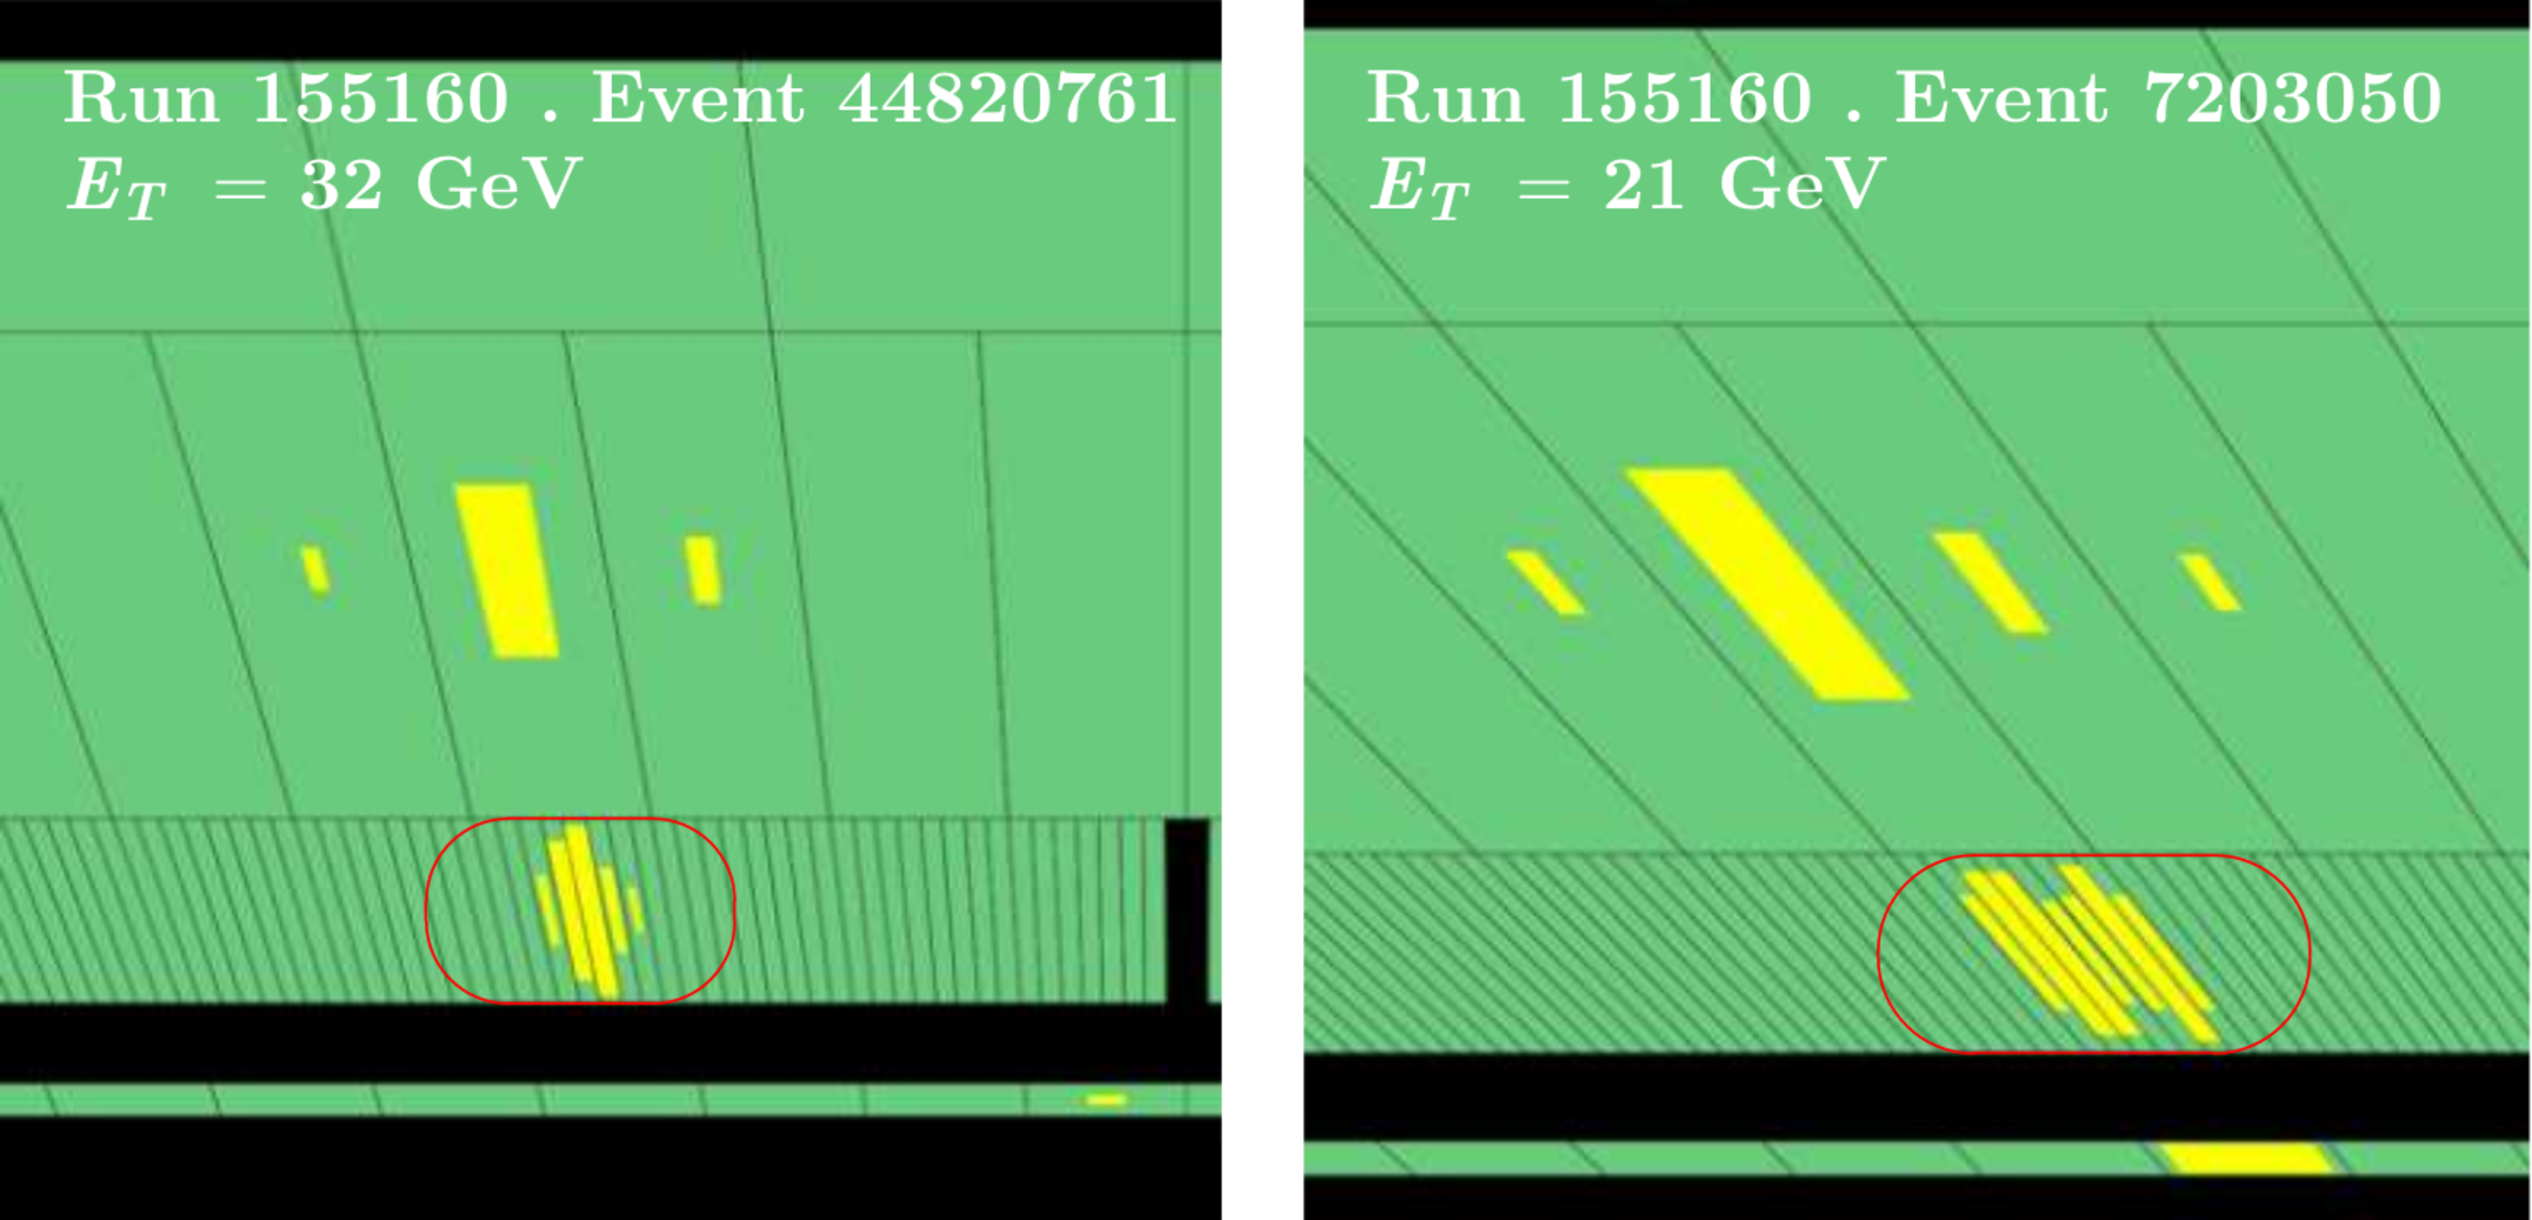
\includegraphics[width=0.8\textwidth]{photon_vs_pion}

  \caption{Deposiciones de energía típicas para un fotón aislado (izquierda) y para un $\pi^0$ decayendo a dos fotones (derecha).}
  \label{fig:photon_pi0}
\end{figure}




\begin{itemize}\itemsep0.2cm\parskip0.2cm
\item Perfil lateral de energía en $\eta$

  \begin{equation}
    F_\mathrm{side} = \frac{E(\pm 3) - E(\pm 1)}{E(\pm 1)}
  \end{equation}
  %
  mide la contención lateral de la cascada electromagnética a lo largo de $\eta$.
  $E(\pm n)$ es la energía en las $\pm n$ celdas alrededor de aquella con la deposición máxima.

\item RMS del perfil lateral de energía en $\eta$ (3 strips)

  \begin{equation}
    w_{s,3} = \sqrt{ \frac{\sum E_i (i - i_\mathrm{max})^2}{\sum E_i} }
  \end{equation}
  %
  mide el ancho de la lluvia electromagnética a lo largo de $\eta$ en la primera capa
  del calorímetro electromagnético usando solo la banda con mayor deposición de energía ($E_{i_\mathrm{max}}$)
  y sus vecina inmediatas.

\item RMS del perfil lateral de energia en eta (total)

  $w_{s,\mathrm{tot}}$ esta definida de la misma forma que $w_{s,3}$, pero utiliza todas las bandas de la
  primera capa del calorímetro electromagnética en una ventana $\Delta\eta \times \Delta\phi = 0.0625 \times 0.2$,
  que corresponde aproximadamente a $20 \times 2$ bandas en $\eta \times \phi$.

\item Diferencia al segundo maximo

  \begin{equation}
    \Delta E = (E^{s1}_{2^{\mathrm{do}} max} - E_\mathrm{min}^{s1} )
  \end{equation}
  %
  es la diferencia entre la energía de la banda con la segunda energía más grande ($E^{s1}_{2^{\mathrm{do}} max}$),
  y la mínima energía ($E_\mathrm{min}^{s1}$) entre la anterior y la celda con la máxima deposición. En caso
  de no haber segundo máximo se fija $\Delta E = 0$.

\item Asimetría de los dos máximos locales en $\eta$

  \begin{equation}
    E_\mathrm{ratio} = \frac{ E^{s1}_{1^{\mathrm{st}} max} - E^{s1}_{2^{\mathrm{nd}} max} }{ E^{s1}_{1^{\mathrm{st}} max} + E^{s1}_{2^{\mathrm{nd}} max} }
  \end{equation}
  %
  mide la diferencia relativa entre las energías de las dos celdas con máxima deposición. En caso de no haber segundo máximo
  se fija $E_\mathrm{ratio} = 1$.

\end{itemize}


A partir de estas variables discriminatorias se definen dos conjuntos de cortes: \emph{loose} y
\emph{tight}.
La selección \emph{loose} se basa solo en las formas de la lluvia
en la segunda capa del calorímetro EM y en la energía depositada en el
calorímetro hadrónico, y es utilizada especialmente por el trigger. La selección
\emph{tight} agrega además información de la capa de \emph{strips} del calorímetro, que
provee un buen rechazo de fondo, %jets hadronicos en los cuales el mesón neutro lleva la mayor parte de la energía del jet
además de ajustar los cortes en las
demás variables. Las variables utilizadas en cada conjunto pueden verse detalladas
en la \cref{tab:phel_id}.

Los cortes de cada conjunto de identificación en las variables que
describen la forma de la lluvia son independientes de la energía transversa del
candidato a fotón, pero varían según la pseudo-rapidez reconstruida del fotón,
para tener en cuenta las variaciones en la cantidad de material y la geometría
del calorímetro.
La selección \emph{tight} se optimiza de forma separada para
fotones convertidos y no-convertidos para proveer una eficiencia de
identificación de alrededor de 85\% para candidatos a fotón con energía
transversa $\et>40 \gev$ y un alto rechazo de fondo\cite{Delmastro:1747242}.

%% En áreas donde un modulo de la b-layer esta muerto, los electrones son
%% comúnmente reconstruido como fotones convertidos. Esta ambigüedad es resulta
%% teneinedo en cuenta el mapa de los píxeles muertos como función del tiempo que
%% dura la recolección de datos. Las conversiones con una sola traza falsas (y
%% algunas de dos trazas) son de esta forma reducidas, con solo un mínima reducción
%% de la eficiencia.


\begin{table}[!htbp]

  \centering

  \caption{Definición de las diferentes variables usadas para la selección
    \emph{loose} (L), \emph{medium} (M) y \emph{tight} (T) de fotones y
    electrones. Las cruces $\times$ indican las variables que son utilizadas en
    cada selección. Además de las variables adicionales utilizadas en cada
    caso, también se incrementan los cortes en las mismas.}
  \label{tab:phel_id}

  \begin{tabular}{y{3cm} p{7cm} c | cc | ccc}

    \hline
    &            &                                       & \multicolumn{2}{c}{$\gamma$} & \multicolumn{3}{c}{$e$} \\
    Categoria    & Descripción                                      & Nombre                  & L & T & L & M & T \\
    \hline

  Aceptancia     & $|\eta|<2.37$, excluyendo $1.37<|\eta|<1.52$       & -                       &   & $\times$ &   & $\times$ & $\times$ \\


  Fuga hadrónica & Cociente entre {\et} en la primera capa del
                   calorímetro hadrónico y {\et} del
                   cluster electromagnético
                   ($|\eta|<0.8$ y $|\eta|\geq1.37$)                & $R_{\mathrm{had}_1}$    & $\times$ & $\times$ & $\times$ & $\times$ & $\times$ \\

                 & Cociente entre {\et} en todo el calorímetro
                   hadrónico y {\et} del cluster electromagnético
                   ($|\eta|\leq0.8$ y $|\eta|<1.37$)                & $R_{\mathrm{had}}$      & $\times$ & $\times$ & $\times$ & $\times$ & $\times$ \\


  Calorímetro EM ($2^\mathrm{da}$ capa)  & Cociente entre la suma de las energías de las
                   $3\times7$ celdas y la suma de $5\times 7$
                   celdas, ambas en torno al centro del cluster     & $R_\eta$                & $\times$ & $\times$ & $\times$ & $\times$ & $\times$ \\

                 & Ancho lateral de la lluvia en dirección de
                   $\eta$                                           & $w_{\eta_2}$            & $\times$ & $\times$ & $\times$ & $\times$ & $\times$ \\

                 & Cociente entre la suma de las energías de las
                   $3\times 3$ celdas y la suma de $3\times 7$
                   celdas, ambas en torno al centro del cluster     & $R_\phi$                &   & $\times$ & $\times$ & $\times$ & $\times$ \\


   Calorímetro EM ($1^\mathrm{ra}$ capa) & Ancho lateral de la lluvia en 3 strips alrededor
                  del máximo                                        & $w_{s,3}$               &   & $\times$ &   & $\times$ & $\times$ \\

                & Ancho lateral total de la lluvia                  & $w_{s,\mathrm{tot}}$    &   & $\times$ &   & $\times$ & $\times$ \\

                & Fracción de energía fuera de las 3 strips
                  centrales pero dentro de las 7                    & $F_{\mathrm{side}}$     &   & $\times$ &   & $\times$ & $\times$ \\

                & Diferencia entre la energía de la strip con el
                  segundo mayor depósito y la menor energía entre
                  los dos primeros máximos locales                  & $\Delta E$              &   & $\times$ &   & $\times$ & $\times$ \\

                & Asimetría entre el primer y segundo máximo        & $E_{\mathrm{ratio}}$    &   & $\times$ &   & $\times$ & $\times$ \\


  Detector Interno            & Impactos en el Pixel $\geq 1$ y en el
                  SCT $\geq 7$                                      & -                       &   &   &   & $\times$ & $\times$ \\

                & Parámetro de impacto $\leq \unit[1]{mm}$          & -                       &   &   &   & $\times$ & $\times$ \\


  Calorímetro EM +
  detector Interno         & $\Delta\eta,\Delta\phi$ entre la traza
                  extrapolada al calorímetro y el cluster           & $\Delta\eta,\Delta\phi$ &  &   &   & $\times$ & $\times$ \\

                & Cociente entre la energía del cluster y el impulso
                  de la traza                                       & $E/p$                   &  &   &   & $\times$ & $\times$ \\


  Detector Interno (TRT)           & Impactos en el TRT                                & -                       &  &   &   & $\times$ & $\times$ \\

                & Fracción de impactos de alto umbral en el TRT     & -                       &  &   &   & $\times$ & $\times$ \\
  \hline
  \end{tabular}

\end{table}



\subsubsection{Corrección a las variables de identificación}

%% Significant differences are observed between data and MC in the shower shape
%% (isEM) distributions.

Dado que la simulación del detector no es perfecta, las distribuciones de las variables
discriminatorias utilizadas en la identificación
de fotones presentan algunas diferencias que pueden resultar significativas entre datos y MC.
Estas diferencias pueden parametrizarse a primer orden como variaciones simples
y a partir de estos corregir el MC.
Las diferencias para cada variable discriminatoria (DV$^i$) se calcula
comparando las distribuciones de las mismas en los datos y en una muestra de
Monte Carlo con una mezcla similar de eventos de señal y fondo.
A partir de esto se calcula la diferencia
entre los valores medios, lo que se denomina \emph{fudge-factor} ($\mu^i$)\cite{ATLAS-CONF-2012-123}.

\begin{equation}
  \mu^i = \avg{\mathrm{DV}^i_\text{DATA}} - \avg{\mathrm{DV}^i_\mathrm{MC}}
\end{equation}

Estos factores son utilizados para corregir las variables de las
muestras simuladas, y los cortes de identificación son nuevamente
aplicados a las variables corregidas.
%% La eficiencia de identificación
%% de fotones es por lo tanto ajustadas para igualar las medidas en datos.

%% Una aproximación más sofisticada para obtener estas diferencias consiste
%% en minimizar la función $\chi^2$ entre las distribuciones de datos y MC,
%% mejorando considerablemente el acuerdo, y es
%% el metodo que se utiliza en el analisis.

%% A more
%% sophisticated approach obtains the shifts by minimizing a chi2 between the data
%% and MC distributions. This method is imperfect in that a shift does not take
%% into account differences in the shape of the distributions and in that it
%% assumes that the shifts are the same for signal and background. However it has
%% been shown that it improves the agreement with data significantly and it is
%% therefore recommended for 2010, 2011, and 2012 photon analyses. A set of shifts
%% has been tabulated for the 2010, 2011, and 2012 data-sets, independently. The MC
%% sample corrected in this way are referred to here as the FF-MC. For 2010 the
%% uncertainty on the FF-MC PID efficiency prediction was conservatively tabulated
%% without the use of data-driven methods, by comparing the efficiencies obtained
%% using different selection criteria and carrying out closure tests using
%% distorted samples as detailed in ATL-PHYS-INT-2011-014 and
%% ATL-COM-PHYS-2011-645 in page 19, and finally at lower  in
%% ATL-COM-PHYS-2011-301 in page 78. For the later data periods the uncertainty is
%% determined through comparisons to data-driven methods and in 2011 additional
%% ``Scale Factors'' are recommended.

También es necesario aplicar factores de escala a todos los fotones
identificados en las muestras de MC para tener en cuenta las diferencias
observadas en la eficiencia de identificación respecto a los datos. Estos
factores son derivados de forma separada para fotones convertidos y
no-convertidos y son provistos de forma central por el grupo
\textsc{Egamma} de ATLAS.


\subsubsection{Aislamiento}

Para la selección final de fotones, se aplica además un corte en la energía
transversa de aislamiento {\etiso}.

%% La energía de aislamiento se define como la
%% suma de la energía transversa de los clusters topologicos (apropiadamente calibrada)
%% dentro de un cono en el plano $(\eta, \phi)$ de radio $R$ alrededor del baricentro del cluster.
%% Solo los topoclusters con energía positiva son usados. Los topoclusters
%% incluyen celdas del calorímetro electromagnético y del calorímetro hadrónico, pero
%% las celdas del TileGap3 son explícitamente removidas.
%% La energía del centro del cono en el calorímetro electromagnético ($5\times7$ celdas alrededor el
%% baricentro del objeto) es sustraída de la suma. Luego se aplican correcciones
%% debido a la energía ambiente por la actividad del pile-up calculadas de acuerdo
%% a \cite{Hance:1379530}, mejorando la performance de la variable de aislamiento
%% para alto pile-up \cite{Laplace:1444890}.


%% Se observa una diferencia entre la energía filtrada del fotón en el cono de
%% aislamiento para datos y MC. Por lo tanto, las correcciones aplicadas que se
%% describen en \cite{Hance:1379530} son levemente distintas para datos y MC.
%% Incluso, se observa que existe una dependencia remanente en la energía de
%% aislamiento con el {\pt} del fotón en datos, para lo cual se aplica un factor de
%% corrección extra que se describe en \cref{sec:opt_ph_iso}.

%% La energia de aislamiento
%% depues de aplicarle las correciones tiene que ser menor que 5 {\gev} para
%% pasar la seleccion final.

%% Los fotones pre-seleccionados son entonces lo que tienen un {\pt} mayor a 20
%% {\gev} con $|\eta| < 2.37$, removiendo los que se encuentran en la región del
%% crack $1.37 < |\eta| < 1.52$, donde $\eta$ se mide en el cluster de la segunda
%% capa del calorímetro.

%% \subsection{Correciones para fotones}

%% Algunas correcciones son aplicadas para mejorar el acuerdo entre datos y
%% simulaciones MC del modelado de las lluvias que dejan los fotones al
%% pasar por el detector.


\begin{figure}[!htb]
  \centering

  \resizebox{0.5\textwidth}{!}{
    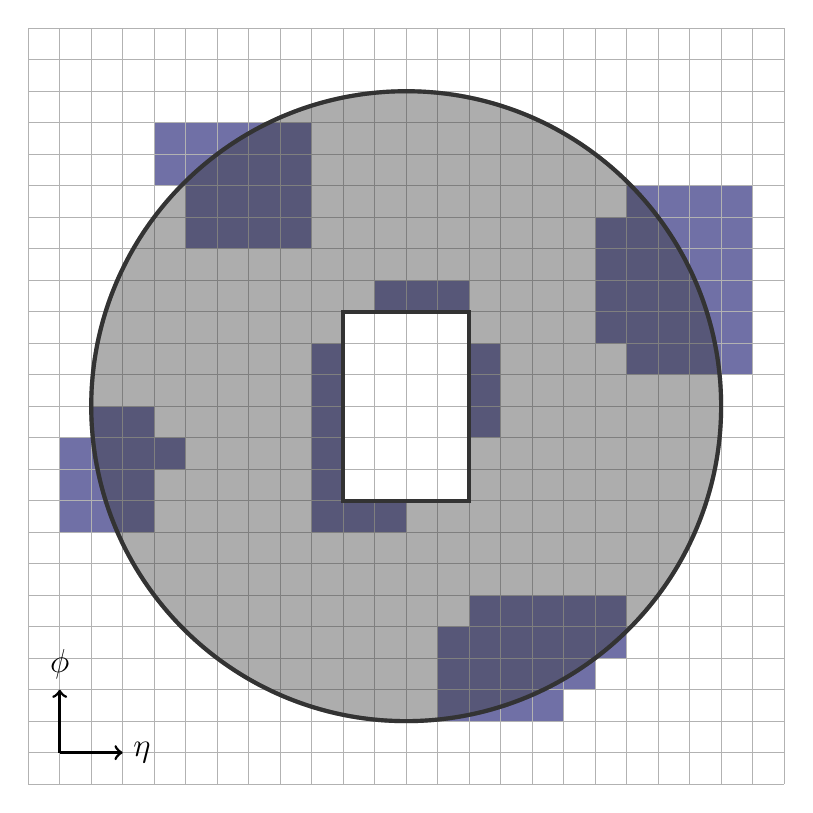
\begin{tikzpicture}

  %% middle
  \draw[blue,fill] (-1.2, -0.4) rectangle (1.2,0.4);
  \draw[blue,fill] (-0.8, -0.8) rectangle (0.8,0.0);
  \draw[blue,fill] (-1.2, 0.4) rectangle (1.2,0.8);
  \draw[blue,fill] (-0.4, -0.8) rectangle (0.4,-1.2);
  \draw[blue,fill] (-0.4, 0.8) rectangle (0.8,1.6);
  \draw[blue,fill] (-1.2, -0.0) rectangle (-0.0,-1.6);

  %% izq arriba
  \draw[blue,fill] (-1.2, 2) rectangle (-2.8,3.6);
  \draw[blue,fill] (-2.8, 3.2) rectangle (-3.2, 3.6);
  \draw[blue,fill] (-2.8, 2.8) rectangle (-3.2, 3.2);

  %% izq abajo
  \draw[blue,fill] (-3.2, -0.4) rectangle (-4.4,-1.6);
  \draw[blue,fill] (-2.8, -0.4) rectangle (-3.2,-0.8);
  \draw[blue,fill] (-3.2, -0.0) rectangle (-4.0,-0.4);

  %% der arriba
  \draw[blue,fill] (2.8, 0.4) rectangle (4.4,2.8);
  \draw[blue,fill] (2.4, 0.8) rectangle (2.8,2.4);

  %% der abajo
  \draw[blue,fill] (0.4, -2.8) rectangle (2.0,-4.0);
  \draw[blue,fill] (0.8, -2.4) rectangle (2.0,-2.8);
  \draw[blue,fill] (2.0, -2.4) rectangle (2.4,-3.6);
  \draw[blue,fill] (2.4, -2.4) rectangle (2.8,-3.2);

  % grid/cone
  \draw[step=0.4,black!30,thin] (-4.8,-4.8) grid (4.8,4.8);

  \draw[black!80, line width=1.5] (0,0) circle (4);
  \draw[black!80, line width=1.5, fill, opacity=0.4] (0,0) circle (4);

  \draw[black!80, line width=1.5, fill=white] (-0.8,-1.2) rectangle (0.8,1.2);
  \draw[step=0.4,black!30,thin] (-0.8,-1.2) grid (0.8,1.2);
  \draw[black!80, line width=1.5] (-0.8,-1.2) rectangle (0.8,1.2);


  \draw[->, line width=1] (-4.4,-4.4) -- (-3.6,-4.4) node[right] {\large $\eta$};
  \draw[->, line width=1] (-4.4,-4.4) -- (-4.4,-3.6) node[above] {\large $\phi$};

 % \draw[dashed, line width=1] (0,0) -- (0,4);
%  \draw[fill] (0,0) circle(0.08);
%  \draw[fill] (0,4) circle(0.08);
 % \node at (0.5,2.5) (R) {\large $R$};
  %\node at (0,2) (mid) {};

  %% \draw[->] (mid) edge[bend right] (R);

\end{tikzpicture}

  }

  \caption{Esquema ilustrando el cálculo de la energía de aislamiento del fotón. La grid representa
    la granularidad de las celdas del calorímetro electromagnético. La energía del candidato a fotón o electrón
    está mayormente contenida en el rectángulo central de $5 \times 7$ en $\Delta\eta \times \Delta\phi$. El
    cono de color gris de radio $R$ rodea al candidato.}
  \label{fig:topoetcone}

\end{figure}


La energía de aislamiento es una herramienta poderosa para distinguir electrones
y fotones directos (producidos en las colisiones) de los falsos candidatos o
fotones y electrones no directos provenientes de jets (producidos de
decaimientos de hadrones). Esta energia de aislamiento se estima a partir de la energía depositada en un
cono alrededor del candidato a electrón o fotón. Para fotones y electrones
directos, no hay energía depositada en este cono aparte de los objetos de baja
energía provenientes de los remanentes de la colisión, interacciones múltiples y
ruido de pile-up. El ruido electrónico del calorímetro también contribuye al
aumento de la energía de aislamiento.

En cambio, para los candidatos falsos y no-directos se observa una energía adicional
(potencialmente grande) en dicho cono proveniente de los objetos que los acompañan en el jet.

En la \cref{fig:topoetcone} se ilustra de forma esquemática como se construye
la variable de aislamiento. Se considera un cono alrededor del candidato
de un tamaño $R$ (generalmente 0.2 o 0.4) y se suma la energía de todas las
celdas que pertenecen a un cluster topológico. Los clusters topológicos son
construidos usando el cociente senal-fondo de energía y sus vecinos próximos,
y son tomados a la escala electromagnética (sin calibrar). La variable final de
aislamiento es construida sumando la energía transversa de los clusters con
energía positiva cuyo baricentro yace dentro del cono de aislamiento. A esta
energía se le resta la energía de las celdas del calorímetro en un rectángulo de
$5\times 7$ celdas (en $\Delta\eta \times \Delta\phi$ en la segunda capa del
calorímetro) centrado en el candidato, a fin de remover la energía del propio
fotón o electrón.

A pesar que este método es muy eficiente, una fracción de la energía (que aumenta con {\pt}) se filtra fuera de
este rectángulo y es necesario aplicar una peque\~na corrección adicional
basada en Monte Carlo.


\subsection{Identificación de electrones}
\label{sec:elec_obj}

Criterios similares de calidad a los descriptos en la sección anterior
se aplican a todos los candidatos a electrones para identificar candidatos
falsos debido a problemas instrumentales.

La energía de los electrones es reconstruida a partir de clusters en el calorímetro
electromagnético sin tener en cuenta su masa, mientras que la información del
detector de trazas es usada para reconstruir su dirección. La escala de energía
en MC es corregida para igualar la observada en datos.

Para electrones se definen tres conjuntos de cortes de identificación: \emph{loose}, \emph{medium} y
\emph{tight}. Estos se describen con más detalle en \cite{ATL-PHYS-PUB-2011-007}, y
en la \cref{tab:phel_id} pueden verse las variables discriminatorias utilizadas
en cada uno.

La eficiencia de identificacion fue medida utilizando electrones de los
decamienitos de $J/\psi\to ee$ y $Z\to ee$ y se combinan para aumentar la
precisión de resultados. Esta eficiencia tiene una alta dependencia con {\et} y, para
los criterios más ajustados también con $\eta$, y varía entre 96\% para el criterio
\emph{loose} y 78\% para el criterio \emph{tight} para electrones con $\et>15\gev$.
Al igual que en el caso de los fotones, se aplican factores de escala
a los electrones del MC para corregir las diferencias observadas en la
eficiencia entre datos y MC.


\section{Muones}
\label{sec:muon_obj}

Los candidatos a muon son reconstruidos usando el algoritmo de reconstrucción
\textsc{staco}\cite{ATLAS_TDR1} que combina la información del detector de
trazas del espectrómetro de muones y el detector interno.

Los muones son clasificados en dos categorías. La primera es denominada
\emph{combined}, y en este caso la reconstrucción de los candidatos a muon
comienza en el espectrómetro de muones, donde se reconstruyen
los segmentos de sus trazas a partir de los impactos en el detector.
Cuando se identifica una traza a partir de estos segmentos, estos se ajustan,
permitiendo extraer una medida preliminar del momento. Los segmentos de trazas
son luego extrapolados al detector interno donde se busca una traza en el mismo
que coincida con aquella del detector de muones.
Si se encuentra una traza asociada, estas son combinadas utilizando el algoritmo
de combinación estadística (\textsc{staco}). En ausencia de una traza asociada,
la combinación es igualmente aceptada si el $\chi^2$ global es menor a un umbral
máximo.

La segunda clasificación comienza buscando trazas en el detector interno que
luego son extrapoladas al espectrómetro de muones y asociadas a, al menos, un
segmento de traza en el MDT o CSC. Estos muones son llamados
\emph{segment-tagged}.

Para la identificación de muones se implementan tres conjuntos de cortes
optimizados para suprimir de forma eficiente trazas falsas y muones que son a
veces creados de una alta multiplicidad de impactos en el MS en eventos donde
algunas partículas de jets muy energéticos llegan al sistema de muones.
Asimismo, discrimina en contra de fondo de muones de decaimientos leptónicos de hadrones
pesados. Siguiendo una aproximación similar a la de electrones, se
definen los tres conjuntos de cortes: \emph{loose}, \emph{medium} y \emph{tight}.
Esencialmente, estos definen el umbral de {\pt}, el requerimiento en el número
de impactos, el parámetro de impacto lateral y longitudinal con respecto al
vértice primario para rechazar posibles rayos cósmicos, entre otros. Los
criterios de identificación detallados pueden verse en \cite{MuonEff}.

%Todos los cortes de identificacion
%provienen de las recomedndaciones propuestas por el grupo de muones \cite{MCPTwiki}.
%% Se pide que los muones sean \textit{Combined}, donde el muon es reconstruido
%% independientemente en el espectrometro de muones y en el detector interno, o
%% \textit{Segment-tagged}, donde el MS es usada para taggear trazas del ID
%% como muones, sin requerir una reconstruccion total de la traza en el MS.

%% %% El momento transverso reconstruido en ambos detectores (ID y MS)
%% %% es esmeareado en MC para reproducir la resolucion del momento en datos.
%% %% Todos los muones reconstruidos con $\pt>6 \gev$ (despues del smearing) y $|\eta|<2.5$
%% %% se consideran candidatos.
%% Ademas, se pide que los candidatos pasen un criterio de calidad \textit{Loose}.
%% %%\footnote{\url{https://twiki.cern.ch/twiki/bin/viewauth/AtlasProtected/QualityDefinitionStaco}},
%% más algunas criterios de calidad en el detector interno de trazas como se describe a continuacion:
%% \begin{itemize}\itemsep0.1cm
%% \item[-] La traza en el ID debe tener un hit en la b-layer, a menos que el modulo de la b-layer este muerto.
%% \item[-] La suma del número de pixel hits y crossed dead pixel sensors must be greater than one.
%% \item[-] La suma del número of SCT hits and crossed dead SCT sensors must be at least six.
%% \item[-] La suma del número of pixel and SCT holes must be less than three.
%% \item[-] Si la traza en el ID estra dentro de la aceptancia del TRT, se pide:
%%   \begin{itemize}\itemsep0.1cm
%%   \item[-] $n = n_{TRT}^{hits} + n_{TRT}^{outliers}$
%%   \item[-] Caso 1: $|\eta| < 1.9$. Require $n > 5$ and $n_{TRT}^{outliers} < 0.9n$.
%%   \item[-] Caso 2: $|\eta| \geq 1.9$. If $n > 5$, then require $n_{TRT}^{outliers} < 0.9n$.
%%   \end{itemize}
%% \end{itemize}

Se requiere ademas que los candidatos a muon pasen un criterio de aislamiento de
la traza: que la suma del {\pt} de las trazas, excluyendo la traza del muon, en
un cono de $\Delta R < 0.3$ sea menor que \unit[12]{\%} del {\pt} del muon. Las
trazas tiene que tener cuatro impactos en el detector de silicio y el parámetro
de impacto a lo largo de la línea del haz ($z_{0}$) debe ser de menos de
$\unit[10]{mm}$.
%% El corte en el {\pt} de muones para el
%% veto se sube a $25 \gev$.
Es necesario aplicar factores de corrección para que la eficiencia en el MC
sea igual a la medida en datos a partir del decaimiento $Z\to\mu\mu$, los
cuales son provistos por el grupo de performance de muones de ATLAS.



\section{Jets}
\label{sec:jet_obj}

Los partones originados en una colisión $pp$, se observan en el detector como
jets de hadrones estables resultado de la hadronizacion de los mismos. Estos
jets atraviesan el detector interno, donde los hadrones cargados dejan su traza,
antes de depositar su energía en los calorímetros electromagnético y hadrónico.
Dada la complejidad de estos objetos, es necesario contar con un una definición
de los mismos, es decir, un algoritmo de reconstrucción.

Los jets hadrónicos utilizados en los análisis de ATLAS son reconstruidos utilizando
un algoritmo de reconstrucción que empieza con los depósitos de energía de las lluvias
electromagnéticas y hadrónicas en los calorímetros. El cuadrimomento es reconstruido
a partir de la energía y los ángulos respecto al vértice primario.

Como en el caso de electrones y fotones, los depósitos de energía en los
calorímetros son agrupadas en clusters. En este caso los clusters son
preseleccionados a partir de las celdas calorimétricas que tengan depósitos de
energía con una magnitud mayor en al menos 4$\sigma$ del ruido esperado en las
celdas. Las contribuciones de energía de todas las celdas vecinas a las celdas
preseleccionadas (en 3 dimensiones) son sumadas a la energía de la celda
preseleccionada, formando un pre-cluster. A continuación, si la energía
depositada en una de las celdas vecinas a la celda preseleccionada es mayor a
2$\sigma$ por encima del valor de fondo de las celdas, estas son agregadas al
pre-cluster. Finalmente se agrega una capa de celdas que rodean el pre-cluster
formando lo que se llama un cluster topológico, o topo-cluster.
Estos topo-clusters son usados por los algoritmos
utilizados para encontrar jets.

Existen muchos algoritmos para la reconstrucción de jets, con sus ventajas y
desventajas. Los jets utilizados en este análisis son reconstruidos usando el
algoritmo anti-$k_t$\cite{Cacciari:2008gp} con un parámetro de distancia $D =
0.4$ en el espacio $(\eta, \phi)$ a partir de clusters calorimétricos
topológicos\cite{Lampl:1099735} formados como se describió previamente.

%% El algoritmo anti-$k_t$ es un algoritmo del tipo de recombinacion secuencial.
%% Este construye los jets combinando los objetos iniciales en objetos cada vez mas
%% grandes de acuerdo a una condición bien definida, hasta que esta condicion no es
%% más satisfecha por los restantes objetos.
Este algoritmo hace uso del {\pt} de cada topo-cluster en el evento y su
separación relativa. Para cada par de objetos (los topo-cluster individuales o
varios topo-clusters que hayan sido agrupados por el algoritmo) $i$ y $j$ se
define la cantidad $d_{ij}$:

\begin{equation}
  d_{ij} = \min(p_{\mathrm{T},i}^{-2}, p_{\mathrm{T},j}^{-2}) \frac{\Delta R_{ij}^2}{D^2}
\end{equation}
%
donde $\Delta R_{ij}^2$ es la distancia entre los objetos en el plano {\etaphi},
y $D$ es el parámetro de distancia que describe el tamaño típico del jet
definido por el algoritmo. La iteración es realizada sobre todos los pares
constituyentes y también entre cada objeto y el haz, con la cantidad especial
$d_{iB} = 1/p_{\mathrm{T}}$. Los objetos $i$ y $j$ son unidos si $d_{ij}$ es
menor que $d_{iB}$.
Si $\min(d_{ij}, d_{iB}) = d_{iB}$, el jet $i$ es declarado un un jet final y
removido de la lista de partículas en la nueva iteración. Este proceso es
repetido hasta que todos los objetos sean combinados, completando la
reconstrucción de todos los jets.

% Calibracion de la energia
La calibración de la energía de los jets tiene como objetivo corregir la energía
del jet medida con los calorímetros a la energía verdadera del correspondiente
jet de partículas estables que entra en el detector \cite{Aad:2011he}. Inicialmente, la energía de
los jets es reconstruida a partir de las deposiciones en los calorímetros. Esta
calibración determina correctamente la energía depositada en el detector solo
para lluvias electromagnéticas, por lo que esta escala de energía es denominada escala
EM.
La escala EM fue establecida utilizando medidas con haces de prueba para
electrones en los calorímetros de la zona de \emph{barrel}
\cite{Abat:1900zz,Aharrouche:2010zz,Adragna:2009zz} y \emph{end-cap}
\cite{Pinfold:2008zzb,2004NIMPA.531..481C}.
Para lluvias hadrónicas, la escala EM lleva a la subestimación de la energía del
jet de un 15-55\%, debido a distintos efectos del detector. Entre otros se
encuentran la medición parcial de la energía depositada por los hadrones, las
pérdidas de energía en las regiones inactivas del detector, deposiciones de
energía de partículas no contenidas en el calorímetro, depósitos de energía de
partículas dentro del jet verdadero que no son incluidas en el jet reconstruido.
Para compensar la diferencia entre la energía medida de los objetos puramente EM
y la energía del jet hadrónico, debe aplicarse una calibración adicional para
convertir la escala EM de los calorímetros de ATLAS a la escala hadrónica.
En el caso más simple la energia medida del jet es corregida utilizando
simulaciones MC y esta calibracion es llamada EM+JES.

En este análisis se utiliza una calibración distinta, denominada LCW+JES. Como
primer paso los clusters son calibrados usando el método de calibración por
pesado de clusters locales (LCW), que consiste básicamente en pesar de forma
diferenciada los depósitos de energía que vienen de lluvias en el calorímetro
electromagnético o hadrónico. Estas correcciones se aplican a la energía de los
topo-clusters independientemente del algoritmo utilizado para la reconstrucción
de los jets y son derivadas de simulaciones Monte Carlo. La calibración final en
la energía del jet también incluye la escala de energía (JES) que corrige la
respuesta del calorímetro con la energía verdadera del jet proveniente de MC.

%% Primero los clusters son calibrados usando el metodo de calibracion por pesado
%% de clusters locales (LCW). Para ello como se determina la naturaleza de cada
%% topo-cluster, es decir, si es hadronico o electromagnetico, y cada topo-cluster
%% es corregido basado en esta clasificacion, donde estas correciones se derivan de
%% simulaciones MC. Estas correcciones se aplican a los clusters independientemente
%% del algoritmo utilizado para la reconstrucción de los jets. Luego los jets son
%% reconstruidos utilizando estos topo-clusters ya corregidos. La calibracion LCW
%% mejora la resolucion de energia de los jets aplicando distintos pesos a los
%% depositos de energia de las lluvias electromagneticas y hadronicas.



%% Excepto para el cálculo de {\met} y la limpieza de eventos, donde ningún corte
%% en $\eta$ es aplicado, los jets solo son considerados si están en la región
%% central del detector ($|\eta|<2.8$) y poseen un $\pt > 20\gev$.

%% Como último paso, para reducir la contaminación de candidatos a jets falsos que
%% no provengan de colisiones, y así mejorar la resolución en la reconstrucción de
%% {\met}, los jets que fallen ciertos criterios de calidad (detallados en []) son
%% removidos.

Como último paso, se requiere que todos los jets reconstruidos pasen ciertos
criterios de seleccion, para remover jets que no provengan de colisiones \cite{Aad:2010ad,ATLAS-CONF-2010-038}.


%% All reconstructed jets are required to pass several selection criteria, which re-
%% move specific non-collision backgrounds [97, 98]. Conditions for these non-collision
%% backgrounds are summarised in Table 5.4. Jet quality is assessed using a collection81
%% 5.3. Jets
%% of discriminating variables, which are summarised in Table 5.3.

%% los eventos con al menos
%% un jet que falla alguno de los siguientes criterios de calidad son removidos:

%% \cite{JetCleaning}.

%% \begin{itemize}\itemsep0.1cm
%% \item Si la fraccion de energia en la endcap del calorimetro hadronico
%%   es mayor a 0.5 $\left(\mathrm{HEC}f > 0.5\right)$, el valor absoluto
%%   medido de la calidad del jet es mayor que 0.5 $\left(|\mathrm{HEC}Q| > 0.5\right)$,
%%   y la calidad del jet normalizada calculada como el valor medio de la suma
%%   cuadratica de la energia de las celdas, es mayor que 0.8 ($LArQmean > 0.8$).

%% \item Si el valor absoluto de la energia total en celdas con un valor negativo es
%%   mayor que $\unit[60]{GeV}$ el jet es considerado malo $\left(|\mathrm{neg.}\,E| > \unit[60]{GeV}\right)$.

%%   %%   For this and the previous item, the signal is consistent with sporadic
%% %%   noise in the hadronic endcap calorimeters.

%% \item Si la fraccion de energia electromagnetica es mayor que 0.95
%%   $\left(\mathrm{EM}f > 0.95\right)$, la valor absoluto de la calidad del jet
%%   es mayor que 0.8 (0.8 $\left(|\mathrm{LAr}Q| > 0.8\right)$, and the normalized jet quality is larger than 0.8
%% %%  $LArQmean > 0.8$ for jets with $|\eta| < 2.8$.
%% \item If the electromagnetic energy fraction is less than 0.05
%% %%   $\left(\mathrm{EM}f < 0.05\right)$ and the ratio of the sum \pt\ of the
%% %%   tracks associated to the jets divided by the calibrated jet \pt\ is less than 0.05
%% %%   $\left(\mathrm{ch}f < 0.05\right)$ for jets with $|\eta| < 2$.
%% %%   In the case where the jet has $|\eta| \ge 2$ the jet is considered bad if
%% %%   the electromagnetic energy fraction is less than 0.05 with no requirement on
%% %%   the jet charge fraction.
%% \item Si un jet tiene más del $99\%$ de su energia contenida en una sola capa
%%   del calorimetro $(\mathrm{F}max > 0.99)$ y tiene $|\eta| < 2$, es consistente
%%   con una senal de rayos cosmicos o \hl{beam halo muons}.
%%   \end{itemize}


\subsection{\bjets}
\label{sec:bjet_obj}

%% MC normalization is extracted as described in \cref{sec:CRs}. b-jets are identified using
%% the MV1 jet tagger \cite{} at the 70\% efficiency operating point, corresponding
%% to the requirement $w > 0.7892$ where $w$ is a weight computed from the different discriminating
%% variables forming the jet tagger. The b-tagging efficiencies have been determined by the flavour
%% tagging working group using the \pt\ of muons relative to the axis of the jet ($p_{T}^{rel}$) \cite{ATLAS-CONF-2012-043} and the
%% derived default scale factors (without JVF cut) are applied to Monte Carlo following the official recommendations \cite{bjetsCalib}.
%% In this analysis, only b-tagged jets with $\pt >$~40 GeV and $|\eta| < 2.5$ will be identified as b-jets.
%% An uncertainty on the jet weight and the event weight is calculated propagating the estimated uncertainties
%% on the scale factors. Scale factor uncertainties depend on the kinematics of the jet and also on the jet flavor.

%% Los $b$-jets son identificados utilizando el algoritmo MV1\cite{btagging} con un
%% 70\% de eficiencia. %% , que corresponde a un requerimiento $w > 0.7892$ donde $w$ es
%% un peso calculado de las distintas variables discriminatorias que conforman el
%% algoritmo
%% La eficienciencia de identificacion de b-jets se determino utilizando
%% el {\pt} de muones relativo al eje del jet () ($p_{T}^{rel}$) y los factores de
%% escala derivados son aplicados al Monte Carlo.

Para identificar jets provenientes de quarks $b$ (\bjets) se utilizó el
algoritmo MV1 \cite{ATLAS-CONF-2014-046,btagging}.
Este algoritmo utiliza
información sobre los parámetros de impacto de la traza y los vértices
secundarios reconstruidos en el detector interno para distinguir jets que
contengan hadrones $b$.



%-----
% MET
%-----
\section{Energía faltante transversa}
\label{sec:met_obj}

La conservación del momento en el plano transversal al haz, $x-y$, implica que
el momento transverso en el estado final debe ser cero. Cualquier desbalance es
lo que se llama momento faltante transverso ($\vec{\met}$) puede indicar la
presencia de particulas indetectables como neutrinos o nuevas particulas
estables, o que interactuan debilmente con la materia.

El momento faltante transverso es reconstruida del negativo de la suma del
momento transverso (\pt) de todas las particulas detectadas, y su magnitud se
denomina con el simbolo {\met}, y se la llama energia faltante. La medida de
{\met} depende fundamentalmente del tratamiento y desempeno de los objetos
fisicos reconstruidos como electroes, fotones, muones, taus, y jets, que son
considerados en el calculo.

La energía faltante transversa es calculada con un algoritmo basado en objetos\cite{Khoo:2012749}.
El algoritmo utiliza para el cálculo de la energía faltante, los objetos físicos
reconstruidos y calibrados descriptos en las secciones anteriores. Los depósitos
de energía en el calorímetro (topo-clusters) son asociados a los objetos de alto
{\pt} en el siguiente orden: electrones, fotones, jets y muones. Los depósitos
que no están asociados a ningún objeto son incluidos en el término \emph{soft}.
La energía faltante es calculada entonces como la suma de los distintos
términos:

\begin{equation}
  E^{\mathrm{miss}}_{x(y)} = (E^{\mathrm{miss}}_{x(y)})^e + (E^{\mathrm{miss}}_{x(y)})^\gamma + (E^{\mathrm{miss}}_{x(y)})^{\text{jet}} + (E^{\mathrm{miss}}_{x(y)})^{\mu} + (E^{\mathrm{miss}}_{x(y)})^{\mathrm{soft}}
\end{equation}
%
donde cada término es calculado como el negativo de la suma de los objetos reconstruidos y
calibrados más el término \emph{soft}.

El término de electrones $(E^{\mathrm{miss}}_{x(y)})^e$ incluye electrones que
pasan el criterio de identificación \emph{medium} con $\pt>10\gev$. La
contribución de fotones $(E^{\mathrm{miss}}_{x(y)})^{\gamma}$ utiliza los
fotones que pasan el criterio de identificación \emph{tight} con $\pt>20\gev$.
En la contribución de jets se incluyen los jets con $\pt>20\gev$ en
$(E^{\mathrm{miss}}_{x(y)})^{\text{jet}}$. La contribución de muones son
incluidos en $(E^{\mathrm{miss}}_{x(y)})^{\mu}$ utilizando los muones que pasan
los criterios de identificación descriptos anteriormente con $\pt>10\gev$
exceptuando el criterio de aislamiento. El término restante
$(E^{\mathrm{miss}}_{x(y)})^{\mathrm{soft}}$ es calculado de los topo-clusters
calibrados y las trazas que no son asociadas a ninguno de los objetos
reconstruidos, usando un algoritmo de flujo de energía.

La falta del término de taus significa que los taus decayendo hadrónicamente se
incluyen en el término de jets o el término soft dependiendo del {\pt} del jet
asociado.

Finalmente, la energia faltante {\met} y el ángulo azimutal de la misma
$\phi^\mathrm{miss}$ son calculados como:

\begin{align}
  \met &= \sqrt{ (E^{\mathrm{miss}}_x)^2 + (E^{\mathrm{miss}}_y)^2 } \\
  \phi^{\mathrm{miss}} &= \arctan \left( E^{\mathrm{miss}}_y / E^{\mathrm{miss}}_x \right)
\end{align}


%%\part{Análisis de Datos} % Análisis de Datos o
\chapter{Métodos estadísticos para la búsqueda de nueva física}
\label{cap:estadistica}

Dada la naturaleza probabilística de las colisiones en el LHC y el bajo número
de eventos esperado en las búsquedas de nueva física, es necesario contar con
una poderosa estructura estadística para interpretar los resultados, especialmente
para identificar una nueva señal sobre las posibles fluctuaciones de los fondos
del SM.

En este capítulo se introducen los conceptos básicos necesarios para entender el
tratamiento estadístico de los datos realizado para esta tesis. Está enfocado en
la búsqueda de nueva física en altas energías, su descubrimiento y/o el
establecimiento de límites de exclusión.

Este capítulo utiliza como referencia los libros \cite{Cowan,James}. Muchos de
los métodos estadísticos más avanzados fueron desarrollados especialmente para
el LHC, y se encuentran descriptos en los artículos
\cite{AsymAprox,ReadCLs,medsigNote,Cranmer:2015nia}. Además se utilizaron los
manuales y artículos que describen las herramientas estadísticas utilizadas
\cite{Cranmer:1456844,HistFitter}.


\section{Funciones de distribución de probabilidad}

Un observable $x$ es por naturaleza frecuentista, es decir, si realizamos
el experimento muchas veces, vamos a obtener distintos valores para $x$ y este
conjunto de valores dará lugar a una función densidad de probabilidad (pdf)
de $x$, que llamamos $f(x)$. En el caso más general, se cuenta con una familia
de pdfs $f(x;\btheta)$ a la cual se denomina <<modelo>>, y cuyos parámetros
representan, por ejemplo, parámetros de la teoría física, alguna
propiedad desconocida de la respuesta del detector, o incertezas sistemáticas
del análisis.

A continuación se describen algunas funciones de probabilidad importantes que
serán utilizadas a lo largo de este capítulo.

\subsubsection{Distribución Gaussiana}

La pdf gaussiana (o normal) de una variable continua $x$ ($-\infty < x < \infty$)
se define como:

\begin{equation}
  f(x;\mu,\sigma) = \frac{1}{\sqrt{2\pi \sigma^2}} \exp \left( \frac{-(x-\mu)^2}{2\sigma^2} \right)
\end{equation}

Los nombres de los parámetros están claramente motivados por los valores del
valor esperado y la varianza de $x$, ya que $E[x] = \mu$ y $V[x] = \sigma^2$. Un
caso especial es cuando $\mu=0$ y $\sigma=1$, que se denomina gaussiana
estándar.
La importancia de la distribución normal proviene del Teorema Central del
Límite. El teorema dice que la suma de $n$ variables continuas independientes
$x_i$ con media $\mu_i$ y varianza $\sigma_i^2$ esta distribuida de acuerdo a
una gaussiana con media $\mu = \sum_{i=1}^n \mu_i$ y varianza $\sigma^2 =
\sum_{i=1}^n \sigma_i^2$ en el límite de $n\to\infty$. Esto se satisface (bajo
ciertas condiciones generales) sin importar las pdfs individuales de $x_i$.


\subsubsection{Distribución $\chi^2$}

La distribución $\chi^2$ de una variable continua $z$ ($0 \leq z \leq \infty$) se
define como:

\begin{equation}
  f(z;n) = \frac{1}{2^{n/2}\Gamma(n/2)} z^{n/2-1} e^{-z/2}, \quad n=1,2,\ldots
\end{equation}
%
donde $n$ es llamado el número de grados de libertad.
Dadas $N$ variables $x_i$ gaussianas con media $\mu_i$ y $\sigma_i^2$, la
variable $z = \sum_{i=1}^{N} \frac{(x_i-\mu_i)^2}{\sigma_i^2}$ esta distribuida
de acuerdo a una distribución $\chi^2$ con $N$ grados de libertad.


\subsubsection{Distribución de Poisson}

La distribución de Poisson es una distribución de probabilidad discreta que
describe, a partir de una frecuencia de ocurrencia media, la probabilidad de que
ocurra un determinado número de eventos durante cierto período de tiempo. Un
ejemplo típico que puede ser descripto por esta distribución es el número de
clicks de un contador Geiger en un determinado intervalo de tiempo.

Se la puede pensar como un límite de la distribución binomial cuando el número ($N$)
de experimentos tiende a infinito y la probabilidad ($p$) a cero, pero el producto es
constantes $Np = \nu$. En ese caso la función de probabilidad esta dada por:

\begin{equation}
  \Pois(n;\nu) = \frac{\nu^n}{n!} e^{-\nu}
\end{equation}

Su valor esperado es $E[n] = \nu$ y la varianza $V[n] = \nu$.
Cuando $\nu \to \infty$ la distribución de Poisson converge a una distribución
normal de media $\nu$ y ancho $\sqrt{\nu}$.


\section{Estimadores}

La estimación de parámetros de las distribuciones observadas es una de las
tareas fundamentales del análisis de datos, y puede considerarse como la
medición de un parámetro (que tiene un valor fijo pero desconocido) basado en un
número limitado de observaciones experimentales. Dado el experimento, la
estimación puntual consiste en determinar un valor único lo más próximo posible al
valor verdadero.

Supongamos un conjunto de $N$ observaciones $\bm{x} = (x_1, x_2, \ldots, x_N)$,
donde las medidas $x_i$ son estadísticamente independientes y cada una está
descripta por una función de densidad de probabilidad $f(x;\btheta)$ que no
se conoce, donde $\btheta$ es un conjunto de parámetros con valores
desconocidos, que tienen valor verdadero $\btheta_0$.

Un estimador es una función de los datos observados $\bm{x}$ que provee
valores numéricos, los valores estimados $\hat{\btheta}$, para el vector de
parámetros $\btheta$.

Algunas propiedades que es importante que cumplan los estimadores son:

\begin{itemize}\itemsep0.2cm\parskip0.2cm
\item {\bf Consistencia:} Un estimador se dice consistente (o asintóticamente
  consistente) si converge al valor verdadero $\btheta_{0}$ con el número de
  medidas $N$: $\lim_{N \to \infty} \hat{\btheta} = \btheta_0$.

\item {\bf Sesgo:} El sesgo esta definido como la diferencia entre el valor
  esperado del estimador y el valor verdadero: $E[\hat{\btheta}] - \btheta_0$ y
  un estimador es no sesgado cuando el sesgo es cero.

\item {\bf Eficiencia:} Un estimador es eficiente si su varianza
  $V[\hat{\btheta}]$ es lo más peque\~na posible.
\end{itemize}

Los dos métodos más utilizados para la estimación de parámetros son el de
\emph{likelihood} máximo y el de cuadrados mínimos.


\section{Método del \emph{likelihood} máximo}\label{sec:MLE}

Para $N$ mediciones estadísticamente independientes cada una descripta por una
pdf $f(x, \btheta)$, la pdf conjunta para los valores observados $x$ está dada
por $f(\bm{x}, \btheta) = \prod_i f(x_i, \btheta)$. La función \emph{likelihood}
se define como la pdf conjunta evaluada en los datos observados,

\begin{equation}
  L(\btheta) = f((x_1, x_2, \ldots, x_n); \btheta) = \prod_{i=1}^{N} f(x_i;
  \btheta)
\end{equation}

El estimador de máximo \emph{likelihood} (MLE) de los parámetros {\btheta} son los
valores $\hat{\btheta}$ para los cuales la función \emph{likelihood} $L(\btheta)$ tiene
su máximo global.
%% Una forma intuitiva de ver esto es la siguiente: si asumimos
%% que la pdf y los parámetros son correctos, esperamos valores altos de la función
%% likelihood comparado con otros parámetros que no sean los verdaderos.
%% Los valores estimados $\hat{\btheta}$ de los parámetros se obtienen buscando el
%% máximo global de la función likelihood.
En la práctica, es conveniente trabajar con el logaritmo de la función
\emph{likelihood} (\emph{log-likelihood}), y buscar el mínimo del negativo de esta función:

\begin{equation}
  - \ln L(\btheta) = - \sum_{i=1}^{N} \ln f(x_i; \btheta)
\end{equation}

En el límite asintótico, cuando el número de mediciones $N$ tiende a infinito,
el MLE es consistente, es decir, para cada parámetro $\theta$ el valor estimado
$\hat{\theta}$ converge al valor verdadero $\theta_0$. En este límite también el
MLE es no sesgado y tiene su menor varianza. Esto significa que ningún otro
estimador puede ser más eficiente. Para un número finito de eventos $N$, sin
embargo, el MLE tiene un sesgo proporcional a $1/N$.


Cuando se repite un experimento muchas veces bajo las mismas condiciones, el
número de eventos $N$ de un proceso fluctúa de acuerdo a una distribución
de Poisson alrededor del valor esperado $\nu$. Este término de Poisson puede
incorporarse entonces a la función \emph{likelihood}, obteniendo lo que se llama
<<\emph{likelihood} extendido>>:

\begin{equation}
  L(\nu,\btheta) = \Pois(N;\nu) \, \prod_{i=1}^{N} f(x_i; \btheta)
  \label{eq:likelihood_ext}
\end{equation}


\section{Contrastación de hipótesis}
\label{sec:testhypo}

En las secciones anteriores se describió cómo pueden utilizarse los datos
observados para estimar parámetros. En esta sección se describirá cómo estos
datos experimentales también pueden ser usados para contrastar hipótesis, es
decir, para rechazar una teoría o hipótesis, o también para elegir
entre hipótesis alternativas.

En general, se llama hipótesis nula ($H_0$) a la hipótesis sujeta a prueba y
usualmente corresponde a la hipótesis que consideramos verdadera. Esta hipótesis
es comparada contra una hipótesis alternativa $H_1$, o varias, distintas a $H_0$.

En el caso de búsqueda de nueva física en altas energías, la hipótesis que juega el rol de
hipótesis nula es la hipótesis de que solo los procesos del SM contribuyen a los
datos observados. Esta hipótesis también suele llamarse hipótesis de
<<solo-fondo>>. La hipótesis alternativa es la hipótesis en la cual, además
de los procesos del SM, también contribuyen procesos de nueva física y se
denomina hipótesis de <<se\~nal+fondo>>.

Una hipótesis se dice simple cuando está completamente determinada,
mientras que si tiene uno o más parámetros libres, se dice compuesta.
Cada hipótesis queda determinada por la pdf que describe a los observables bajo
esa hipótesis $f(\bm{x}|H)$.

Una vez definidas las hipótesis, se quiere saber si los datos medidos son
compatibles con la hipótesis nula o si la hipótesis nula puede ser rechazada en
base a estos datos. Con este objetivo se define un <<estadístico de prueba>>
$t(\bm{x})$ que es función de los datos observados. En el caso de considerar un
estadístico de prueba escalar, $t(\bm{x}) \to \mathbb{R}$, éste contendrá toda la
información de discriminación entre $H_0$ y $H_1$ en un solo número.

Cada estadístico de prueba tendrá su pdf asociada $g(t|H)$ y la decisión sobre
la hipótesis estará basada en el valor del estadístico observado $t_\text{obs}$
y la definición de una región critica $R$. La región critica queda
definida por un valor de corte $t_c$ y para el caso de que la hipótesis
alternativa tiende a tener valores de $t$ mayores que bajo $H_0$, la región
critica corresponde a $t \geq t_c$ (ver \cref{fig:stat_test}).

Si el valor observado se encuentra fuera de la región critica (dentro de la
región de aceptancia) la hipótesis $H_0$ no puede ser rechazada, y si está
dentro es rechazada.

\begin{figure}[h]
  \centering
  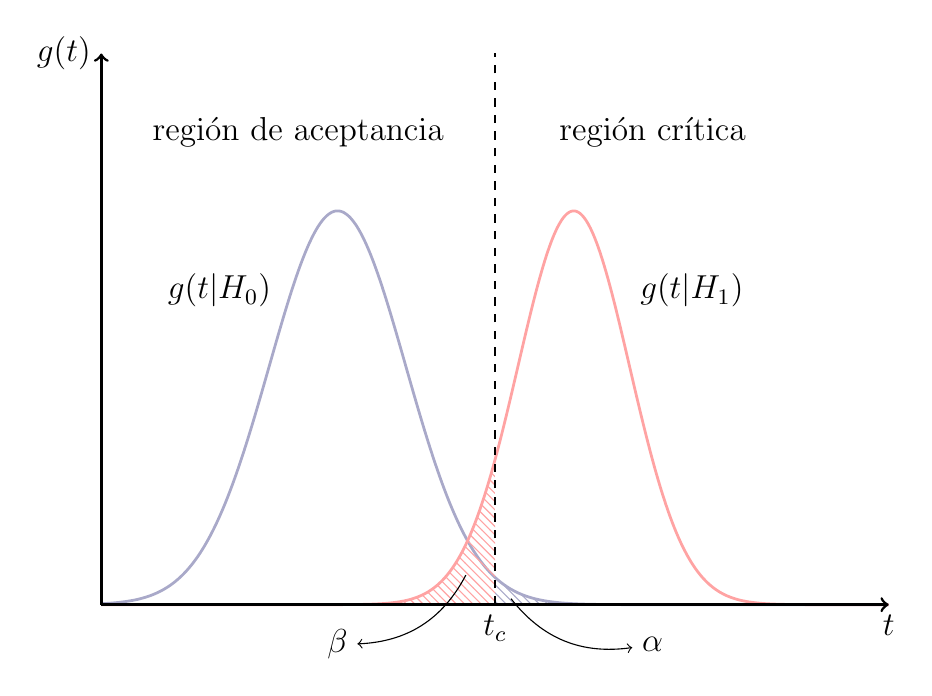
\begin{tikzpicture}

    \colorlet{red}{red!60}
    \colorlet{blue}{blue!60}

    \draw[blue,line width=1] plot[domain=0:10, samples=500] ({\x},{5*exp(-((\x-3)^2/1.5))});
    \fill[blue, pattern=north west lines, pattern color=blue] (5,0) -- plot[domain=5:10, smooth] ({\x},{5*exp(-((\x-3)^2/1.5))}) -- cycle;

    \draw[red, line width=1] plot[domain=0:10, samples=500] ({\x},{5*exp(-((\x-6)^2)/1)});
    \fill[red, pattern=north west lines, pattern color=red] (5,0) -- plot[domain=0:5,smooth] ({\x},{5*exp(-((\x-6)^2)/1)}) -- cycle;

    \draw[line width=1, ->] (0,0) -- (10,0) node[below] {\large $t$};
    \draw[line width=1, ->] (0,0) -- (0,7) node[left] {\large $g(t)$};

    \draw[dashed, line width=0.8] (5, 0) -- (5, 7);
    \draw node at (5,-0.3) {\large $t_c$};

    \draw node at (1.5, 4) {\large $g(t|H_0)$};
    \draw node at (7.5, 4) {\large $g(t|H_1)$};

    \draw node at (2.5, 6) {\large regi\'on de aceptancia};
    \draw node at (7, 6) {\large regi\'on cr\'itica};

    \draw node (alpha) at (3,-0.5) {\large $\beta$};
    \draw node (p0) at (4.7,0.5) {};
    \draw[->] (p0) edge[bend left] (alpha);

    \draw node (beta) at (7,-0.5) {\large $\alpha$};
    \draw node (p1) at (5.1,0.2) {};
    \draw[->] (p1) edge[bend right] (beta);

\end{tikzpicture}

  \caption{Funciones de densidad de probabilidad para el estadístico de prueba
    $t$ bajo la hipótesis nula $H_0$ (azul) y la hipótesis alternativa $H_1$
    (rojo). Las regiones de aceptancia y rechazo quedan definidas por $t_c$.}
  \label{fig:stat_test}
\end{figure}

La probabilidad de rechazar $H_0$ siendo ésta verdadera es denominada tamaño de la
contrastación $\alpha$:

\begin{equation}
  \alpha = \int_{R} g(t|H_0)\, dt
\end{equation}
%
lo cual también determina el nivel de significancia como
$(100 - \alpha) \%$. Este error, de rechazar $H_0$ cuando la hipótesis es verdadera, es llamado
error de tipo I. Por otro lado el error de aceptar $H_0$ cuando es falsa se
llama error de tipo II, y su probabilidad de ocurrencia, $\beta$, depende de la
hipótesis alternativa $H_1$ y del poder del contraste que se define como $(1-\beta)$:

\begin{equation}
1-\beta = \int_R g(t|H_1)\, dt
\end{equation}

En principio, cualquier función de los datos puede ser utilizada como estadístico
de prueba, pero un buen estadístico será aquel para el cual sus distribuciones
para la hipótesis nula y alternativa estén claramente separadas. Para esto se
busca el estadístico de prueba que tenga el mayor poder posible $(1-\beta)$, para un dado
tama\~no $\alpha$.

Para el caso de hipótesis simples, el teorema de Neyman-Pearson\cite{Neyman289} afirma que el
estadístico de prueba con mayor poder para un tama\~no esta dado por:

%% Para el caso de dos hipótesis simples (sin parámetros), el test estadístico con mayor
%% poder esta dado por el \emph{likelihood ratio} $T_\text{NP} = \vec{f}(\mathcal{D}|H_1)/\vec{f}(\mathcal{D}|H_0)$.
%% Este resultado se conoce como lema de Neyman-Pearson.

\begin{equation}
  t(\bm{x}) = \frac{f(\bm{x}|H_1)}{f(\bm{x}|H_0)}
\end{equation}
%
y la mejor región crítica consiste en los $\bm{x}$ que satisfacen $t(\bm{x}) > c_\alpha$
donde $c_\alpha$ es una constante que se ajusta para que el tama\~no sea $\alpha$.
Este estadístico de prueba es esencialmente el cociente de los \emph{likelihoods}
para las dos hipótesis.


El nivel de acuerdo entre los datos observados y una hipótesis $H$ es
cuantificado calculando el <<\pvalue>>, es decir, la probabilidad, bajo la
suposición de que $H$ es cierta, de observar datos de igual o menor
compatibilidad con la predicción de $H$, respecto a los datos observados.

\begin{equation}
  p_H = P(t>t_\text{obs}|H) = \int_{t_\text{obs}}^{\infty} g(t|H) \, dt
\end{equation}
%
donde $t_\text{obs}$ es el valor del estadístico de prueba obtenido con los
datos observados.

De esta forma, un {\pvalue} grande denota que la evidencia en contra de $H_0$ es
débil y un {\pvalue} chico denota que los datos contienen mucha evidencia en
contra de $H_0$.
%% En este sentido de p-valores, se puede no hablar de pruebas de hip´otesis, sino de
%% pruebas de significancia, donde la cuantificaci´on del concepto abstracto de significancia
%% es el p-valor
Se dice que la hipótesis es excluida si el {\pvalue} se encuentra por debajo de un valor
específico dado por el tama\~no del test $\alpha$, donde $\alpha \in [0,1]$.

En física de partículas es usual convertir el {\pvalue} en la significancia
equivalente, $Z$, definida de forma tal que una variable distribuida normalmente
tenga una probabilidad igual a ese {\pvalue} de ser encontrada a más de $Z$
desviaciones estándar a la derecha de su media. Esto es:

\begin{equation}
  Z = \Phi^{-1}(1-p)
\end{equation}
%
donde $\Phi^{-1}$ es el cuantil (la función inversa de la distribución
acumulada) de la distribución gaussiana.

También es útil definir, para poder cuantificar la sensibilidad de un experimento,
la significancia esperada que se obtendría dados los datos observados bajo la
suposición de ciertas hipótesis.
Para esto se calcula la significancia de la hipótesis $H_0$, respecto
a la mediana de la hipótesis $H_1$.


\section{Descubrimiento}

Generalmente, cuando se modela un fenómeno aleatorio de interés, el modelo
elegido para ajustar a las observaciones de dicho fenómeno suele tener varios
parámetros, de los cuales solo algunos pueden ser de interés. De manera formal a
estos parámetros se los denomina <<parámetros de interés>> y al resto, <<parámetros
\emph{nuisance}>>, y conviene separarlos explícitamente $\btheta \to (\mu, \btheta)$.

Para la búsqueda de nueva física es común definir como parámetro de interés a la
intensidad de la señal de forma tal que la hipótesis de solo-fondo corresponde a
$\mu = 0$ , y la hipótesis de señal+fondo a $\mu = 1$.
En general, las incertezas sistemáticas son incluidas en el modelo
utilizando parámetros \emph{nuisance}.

En este escenario, donde hay un único parámetro de interés
$\mu$, y el resto de parámetros \emph{nuisance} $\btheta$, es conveniente
definir el <<\emph{profile likelihood ratio}>> (PLR),

\begin{equation}
  \lambda(\mu) = \frac{L(\mu,\doublehat{\btheta})}{L(\hat{\mu},\hat{\btheta})}
  \label{eq:lambdamu}
\end{equation}
%
donde en el denominador, los valores $\hat{\btheta}$ y $\hat{\mu}$ son los
valores estimados MLE. En el numerador, los parámetros {$\doublehat{\btheta}$}
son los valores que maximizan la función \emph{likelihood} para un valor fijo de $\mu$,
es decir que es una función multidimensional que depende solo del parámetro $\mu$.
Este proceso de elegir valores específicos de los parámetros
\emph{nuisance} para un valor dado de $\mu$ se lo conoce como \emph{profiling}. El PLR
depende explícitamente de $\mu$ pero es independiente de los parámetros
\emph{nuisance} que han sido ``eliminados'' vía el \emph{profiling}.
La presencia de los parámetros \emph{nuisance} que son ajustados a los datos ensanchan
la función \emph{likelihood} como función de $\mu$, respecto a la distribución si sus
valores estuvieran fijos. De cierta forma reflejan una pérdida de información
sobre $\mu$ debido a estos parámetros desconocidos, que suelen ser
las incertezas sistemáticas.

En la sección anterior se mostró que el mejor estadístico de prueba para hipótesis
simples esta dado por el cociente de los \emph{likelihoods} de las dos hipótesis, de acuerdo
al teorema de Neyman-Pearson.
Desafortunadamente no hay un equivalente al lema de Neyman-Pearson para modelos
con muchos parámetros libres. Sin embargo, hay una generalización natural basada
en el PLR. De la \cref{eq:lambdamu} se puede ver que $0 \leq \lambda \leq 1$, y
$\lambda$ cercano a 1 implica un buen acuerdo entre datos y el valor hipotético de $\mu$.
De forma equivalente conviene utilizar como estadístico de prueba $t_\mu = -2 \ln \lambda(\mu)$.
En el límite asintótico ($N\to\infty$) el teorema de Wilk\cite{WilkTheo} muestra
que $-2 \ln \lambda(\mu)$ sigue una distribución $\chi^2$ con un grado de libertad.
Esta propiedad sera útil para aproximar la pdf del estadístico
de prueba (ver \cref{sec:aprox}).


%% Entonces para este  caso de $\mu \geq 0$ conviene definir,

%% \begin{equation}
%%   \tilde{\lambda}(\mu) =
%%     \begin{cases}
%%       \frac{L(\mu, \doublehatfix{\btheta})}{L(\hat{\mu}, \hat{\btheta})} & \hat{\mu} \geq 0 \\
%%       \frac{L(\mu, \doublehatfix{\btheta})}{L(0, \hat{\btheta}(0))} & \hat{\mu} < 0
%%     \end{cases}
%% \end{equation}

%% Acá $\doublehat{\btheta}(0)$ y $\doublehat{\btheta}(\mu)$ se refieren a los MLE
%% de {\btheta} dados los parámetros de intensidad de señal parámetro de 0 o $\mu$
%% respectivamente. El correspondiente estadístico de prueba puede obtenerse como,

%% \begin{equation}
%%   \tilde{t}_\mu = -2 \ln \tilde{\lambda}(\mu) %% \begin{cases} %% -2 \ln  \frac{L(\mu, \hat{\hat{\bm{\theta}}})}{L(0, \hat{\bm{\theta}}(0))} & %%
%%   %%-\hat{\mu} < 0 \\ %%2 \ln \frac{L(\mu, \hat{\hat{\bm{\theta}}})}{L(\hat{\mu}, %%     -\hat{\bm{\theta}})} & \hat{\mu} \geq 0 %% \end{cases}
%% \end{equation}

Un caso de especial importancia del estadístico $t_\mu$ es cuando $\mu=0$.
Rechazar la hipótesis de $\mu=0$ es lo
que llamamos descubrimiento de una nueva señal.
Aunque es cierto que un valor de $\hat{\mu}$ mucho menor a cero representa
evidencia contra el modelo de solo-fondo, este tipo de discrepancia no muestran
que los datos contengan eventos de señal. Es por este motivo que solo se
considera que los datos no tienen un buen acuerdo con la hipótesis de solo-fondo
cuando $\hat{\mu}$ es mayor a cero.
Para este caso se define $q_0$ como,

\begin{equation}
  q_0 =
  \begin{cases}
    -2 \ln \lambda(0) & \hat{\mu} > 0 \\
    0 & \hat{\mu} \leq 0
  \end{cases}
\end{equation}

Si los datos fluctúan de tal manera que haya menos eventos que los predichos por
el fondo, entonces $\hat{\mu} = 0$ y $q_0=0$. A medida que el número de
eventos crece por encima del número de eventos de fondo esperado (mayor
$\hat{\mu}$) el valor de $q_0$ es mayor, lo que corresponde a un incremento en
el nivel de incompatibilidad con la hipótesis de solo-fondo. Para cuantificar el
nivel de desacuerdo entre datos y la hipótesis de $\mu=0$ usando el valor
observado de $q_0$ se calcula el {\pvalue} como,

\begin{equation}
  p_0 = \int_{q_{0}^{\text{obs}}}^{\infty} f(q_0|\mu=0) \, dq_0
  \label{eq:p0}
\end{equation}

En el caso que $p_0 \leq \epsilon$ donde $\epsilon$ es un tamaño del test
fijado anteriormente, se dice que hay un descubrimiento. En general en física de
altas energías suele utilizarse $\epsilon = 2.87 \times 10^{-7}$, el cual
corresponde a una significancia equivalente $Z=5\sigma$.

Es importante notar que el hecho de rechazar la hipótesis de solo-fondo en un
sentido estadístico es solo parte de descubrir un fenómeno nuevo.
Para confirmar la presencia de este nuevo fenómeno es necesario estudiar
el acuerdo de este para describir los datos observados.


\section{Límites de Exclusión}
\label{sec:limits}

Si $p_0> \epsilon$ no se puede rechazar $H_0$. Esto no
significa que todos los valores de $\mu$ bajo $H_1$ estén excluidos.
En particular, hay valores de $\mu$ a los que el análisis no es sensible
y valores que los datos observados no permite excluir.

Para establecer límites superiores en el parámetro $\mu$ se considera
$q_\mu$,

\begin{equation}
  q_\mu =
  \begin{cases}
    -2 \ln \lambda(\mu) & \hat{\mu} \leq \mu \\
    0 & \hat{\mu} > \mu
  \end{cases} \label{eq:qmu}
\end{equation}

La razón para poner $q_\mu = 0$ para $\hat{\mu} > \mu$ es que cuando se
establece un límite superior, el hecho de que $\hat{\mu} > \mu$ representa menos
compatibilidad con $\mu$ que los datos obtenidos, y por lo tanto no se considera
parte de la región de rechazo de la contrastación.

También es importante notar que $q_0$ (utilizado como estadístico de prueba para
descubrimiento) no es simplemente un caso especial de la
\cref{eq:qmu}, sino que tiene una definición diferente. Es decir, $q_0$ es cero
si los datos fluctúan hacia abajo ($\hat{\mu}<0$), pero $q_\mu$ es cero si los
datos fluctúan hacia arriba ($\hat{\mu}>\mu$).

%%Para los datos observados se tiene $\tilde{q}_\mu^\text{obs}$.
%% Para generar la
%% distribución de $\tilde{q}_\mu$ se pueden generar pseudo-experimentos con Monte
%% Carlo $\to$ $f(\tilde{q}_\mu|\mu, \btheta)$.

%% El {\pvalue} para una observación bajo una hipótesis $\mu$ es la
%% probabilidad de obtener un resultado igual o más extremo que los obtenidos dado
%% H.

%% \begin{equation}
%%   p_{(\mu,\btheta)} = \int_{q_{\mu,\text{obs}}}^{\infty}
%%   f(q_\mu|\mu,\btheta) \, dq_\mu
%% \end{equation}
%% \begin{equation}
%%   p_{\mu} = \int_{q_{\mu,\text{obs}}}^{\infty}
%%   f(q_\mu|\mu) \, dq_\mu
%% \end{equation}

%% Este {\pvalue} presenta como dificultad que no solo depende del parámetro de interés,
%% sino también de $\btheta$. La hipótesis no puede ser rechazada a menos que
%% el {\pvalue} sea suficientemente chico para todos los valores de $\btheta$. De forma
%% equivalente se utiliza el supremo del {\pvalue} para decidir si la hipótesis de $\mu = \mu_0$
%% es aceptada o rechazada.

%% \begin{equation}
%%   p_\mu^\text{sup} = \sup_\theta p_{(\mu,\btheta)}
%% \end{equation}

%% La mayor razón para usar PLR como estadístico de prueba es que en el límite de muchos
%% eventos la distribución del PLR $\lambda(\mu=\mu_\text{0})$ es independiente
%% de los valores de los parámetros nuisance $p_\mu^\text{sup} = p_{(\mu,\btheta)}
%% \, \forall \theta$. Esto es una consecuencia del Teorema de Wilk.
%% Elegir $\btheta^\text{sup} = \doublehat{\btheta}(\mu)$, es decir, el valor para el
%% cual $p_{(\mu,\btheta)} = p_\mu^\text{sup}$ es un buen valor estimado de
%% $\btheta^\text{sup}$.

Para cuantificar la consistencia de los datos observados con la hipótesis de
intensidad de se\~nal $\mu$ se calcula el {\pvalue}

\begin{equation}
  p_\mu = \int_{q_{\mu}^{\text{obs}}}^{\infty} f(q_\mu|\mu) \, dq_\mu \equiv \clsb
  \label{eq:pmu}
\end{equation}
%
donde valores chicos de $p_\mu$ indican baja compatibilidad con la hipótesis
de señal+fondo.

El límite superior con un nivel de
confianza del 95\% se obtiene resolviendo la siguiente ecuación:

\begin{equation}
  p_{\mu_\text{up}} = 0.05
\end{equation}

Sin embargo, el límite superior calculado de esta forma tiene un problema: de
acuerdo a este, se dice que una señal está excluida a 95\% CL, si ${\clsb} \leq
0.05$. Si se considera el caso de $\mu=0$, se espera que por construcción el
{\clsb} sea menor o igual que 0.05 con una probabilidad de 5\%. Esto significa
que el 5\% de los análisis estarían excluyendo modelos con cero señal. Otro
problema del {\clsb} es que para dos experimentos con el mismo número chico de
eventos de señal esperado pero con un número de eventos de fondo distinto, el
experimento con mayor fondo va a imponer mejores límites.

Con motivo de solucionar estos inconvenientes se introduce el método de {\cls}\cite{ReadCLs}.

%% Los intervalos de confianza frecuentistas cubren e
%% Un límite superior con 95\% de nivel de confianza cubre al valor verdadero con una probabilidad de
%% 95\%. Eso sinifica que un 5\% de las veces no lo cubre. Esto significa, que si no hay senal, el 5\% de las veces
%% se esta excluyendo cualquier valor positivo de XS.

\begin{equation}
  \cls = \frac{p_\mu}{1-p_b}  \equiv \frac{\clsb}{\clb}
\end{equation}
%
donde $p_b$ es el valor del mismo estadístico bajo la hipótesis de solo-fondo,

\begin{equation}
  1 - p_b = \int_{q_\mu^\text{obs}}^{\infty}
  f({q}_\mu|0) \, dq_\mu \equiv \clb
\end{equation}

El límite superior {\cls} en $\mu$, $\mu_\text{up}$ se obtiene resolviendo
$\cls = 0.05$. Se rechazan los valores de $\mu$ si $\mu <
\mu_\text{up}$ con un nivel de confianza de 95\%.

Cabe mencionarse para una observación cercana al número de eventos esperado de solo-fondo ($\clb
\sim 0.05$) el {\cls} da un valor del orden de dos veces el obtenido utilizando
el {\clsb}.


% -----------------------
% Aproximacion asintotica
% -----------------------
\section{Aproximación asintótica}\label{sec:aprox}

Para poder calcular el {\pvalue} de una hipótesis utilizando las ecuaciones
\eqref{eq:p0} y \eqref{eq:pmu} es necesario conocer las distribuciones muestrales
del estadístico de prueba, $f(q_\mu)$.

Como se dijo anteriormente, el teorema de Wilk establece que para el límite de
$N\to\infty$, el estadístico de prueba $t_\mu = -2\ln \lambda$ sigue una
distribución $\chi^2$ con un grado de libertad, cuando la hipótesis nula es verdadera.

El teorema de Wald\cite{WaldTheo} generaliza este teorema para el caso de la hipótesis no nula.
En este caso el estadístico $-2\ln\lambda$ sigue una distribución $\chi^2$ no central.
A partir de este resultado puede mostrarse que para el caso de un solo parámetro de interés vale:

\begin{equation}
  -2 \ln \lambda(\mu) = \frac{(\mu - \hat{\mu})^2}{\sigma^2} + \mathcal{O}(1/\sqrt{N})
\end{equation}
%
donde $\hat{\mu}$ sigue una distribución normal con media $\mu'$ y desviación
estándar $\sigma$. Si $\hat{\mu}$ se encuentra distribuido normalmente y se
desprecian los términos $\mathcal{O}(1/\sqrt{N})$, se puede mostrar que en el
régimen asintótico, el estadístico $q_\mu$ sigue una distribución $\chi^2$ no
central con un grado de libertad.

Entonces, en el límite asintótico, el estadístico $q_\mu$ puede aproximarse por

\begin{equation}
  q_\mu =
  \begin{cases}
    \frac{(\mu-\hat{\mu})^2}{\sigma^2} & \hat{\mu} \leq \mu \\
    0 & \hat{\mu} > \mu
  \end{cases}
\end{equation}
%
y el {\pvalue} de la hipótesis $H_\mu$ es,

\begin{equation}
  p_\mu = \int_{q_{\mu}^{\text{obs}}}^{\infty} f(q_\mu|\mu) \, dq_\mu = 1 - \Phi(\sqrt{q_\mu})
\end{equation}
%
y su correspondiente significancia equivalente,

\begin{equation}
  Z_\mu = \Phi^{-1}(1-p_\mu) = \sqrt{q_\mu}
\end{equation}

Siguiendo los mismos argumentos, el estadístico $q_0$ puede aproximarse con,

\begin{equation}
  q_0 =
  \begin{cases}
    \frac{(\hat{\mu})^2}{\sigma^2} & \hat{\mu} \geq 0 \\
    0 & \hat{\mu} < 0
  \end{cases}
\end{equation}

El {\pvalue} para $H_0$ entonces es,

\begin{equation}
  p_0 = \int_{q_{0}^{\text{obs}}}^{\infty} f(q_0|0) \, dq_0 = 1 - \Phi(\sqrt{q_0})
\end{equation}
%
y la correspondiente significancia,

\begin{equation}
  Z_0 = \Phi^{-1} (1-p_0) = \sqrt{q_0}
\end{equation}

Estas aproximaciones permiten conocer las distribuciones muestrales y calcular
valores-$p$ y significancias en el caso de un gran número de datos, de una forma
simple y computacionalmente poco costosa. A pesar de que estrictamente es válido
para $N\to\infty$, esta aproximación es suficientemente precisa para un número
de eventos de fondo $\gtrsim \mathcal{O}(10)$.

Para muestras de datos muy pequeñas, o en casos donde la precisión es
importante, siempre pueden validarse estas aproximaciones utilizando la
generación Monte Carlo.
Para esto es necesario utilizar simulaciones Monte Carlo para generar lo que se
denomina <<pseudo-experimentos>>. El procedimiento consiste en generar el
conjunto de observables $\bm{x}$ utilizando la pdf $f(\bm{x}|H)$ y calcular el
valor del estadístico de prueba $t(\bm{x})$ para cada conjunto. Este proceso se
repite hasta acumular suficiente estadística en la distribución muestral del
estadístico $g(t|H)$.



% ----------------------
% Significancia esperada
% ----------------------
\section{Significancia esperada}

En física de partículas la cantidad $s/\sqrt{b}$ ha sido siempre utilizada como
una medida de la significancia esperada de descubrimiento\cite{medsigNote}. La
explicación detrás de esta formula es que una cantidad $n$ que sigue una
distribución de Poisson con una media grande $s+b$ puede ser aproximada por una
variable $x$ distribuida según una gaussiana con media $s+b$ y desviación
estándar $\sqrt{s+b}$. En este caso el {\pvalue} de la hipótesis de solo-fondo
dada una observación $x$ esta dado por,

\begin{equation}
  p = 1 - \Phi \left( \frac{x-\mu}{\sigma} \right) = 1 - \Phi \left(
  \frac{x-b}{b} \right)
\end{equation}
%
donde $\mu=b$ y $\sigma = \sqrt{b}$ se refieren a la media y la desviación
estándar de $x$ suponiendo que $s=0$. Traduciendo este {\pvalue} a significancia,

\begin{equation}
  Z = \frac{x-b}{b}
\end{equation}

La significancia esperada, a diferencia de la observada, se calcula desde la mediana
de la hipótesis alternativa. Entonces como la mediana de la hipótesis de señal+fondo,
en este caso igual a la media, es $s+b$,

\begin{equation}
  Z_\text{exp} = \frac{s}{\sqrt{b}}
  \label{eq:Zsimple}
\end{equation}
%
que es la ecuación conocida.

%% utilizando la aproximación
%% asintotica de la seccion anterior,
De forma general, para el caso de un número de eventos de fondo $b$ conocido con
una incerteza despreciable, se puede escribir la función \emph{likelihood} como,

\begin{equation}
  L(s) = \frac{(s+b)^n}{n!} e^{-(s+b)}
\end{equation}
%
y utilizando la aproximación asintótica, la significancia de descubrimiento
puede ser aproximada por $Z=\sqrt{q_0}$, lo que da como resultado,

%% \begin{equation}
%%   Z = \sqrt{2\left( n \ln \frac{n}{b} +b -n \right)}
%%   \label{eq:Z}
%% \end{equation}
%
%% para $n>b$ y $Z=0$ para $n<b$. También puede aproximarse la significancia esperada
%% reemplazando los datos por el conjunto de datos de Asimov. Substituyendo $s+b$
%% por $n$ en la {\eq} \eqref{eq:Z}, la aproximaxion de Asimov para la
%% significancia esperada $Z_A$ es,

\begin{equation}
  Z_A = \sqrt{2\left( (s+b) \ln \left( 1 + \frac{s}{b}\right) - s \right)}
  \label{eq:Z}
\end{equation}

Si se expande el logaritmo en la ecuación anterior en $s/b$ se tiene $Z_A =
s/\sqrt{b} + \mathcal{O}(s/b)$ que es la expresión de la \cref{eq:Zsimple}
y es válida solo en el límite $s \ll b$.

Si el número de eventos esperado de fondo $b$ no es conocido, uno debe incluirlo
como un parámetro \emph{nuisance} en la función \emph{likelihood}. Pero como $b$ puede
ajustarse para cualquier número de eventos, es necesario introducir información
adicional para restringir $b$. En general se suele hacer mediante una medida
auxiliar, mirando el número de eventos observados $m$ en una región de control
donde se supone ausencia de señal, y considerando que $m$ sigue
una distribución de Poisson con media $\tau b$, donde $\tau$ es un factor de
extrapolación.

La función \emph{likelihood} total es el producto de las dos distribuciones de Poisson
correspondientes a cada región:

\begin{equation}
  L(s, \btheta) = \Pois (n;s+b) \, \Pois(m;\tau b)
\end{equation}

Utilizando la aproximación $Z = \sqrt{q_0}$, válida en el límite de una muestra
grande de datos y teniendo en cuenta que los valores esperados son $s+b$ y $\tau b$
para obtener la significancia esperada, se tiene:

\begin{equation}
  Z_A = \left[ 2 \left( (s+b) \ln \left[ \frac{s+(1+\tau)b}{(1+\tau)(s+b)}
      \right] + \tau b \ln \left[ 1 + \frac{s}{(1+\tau)b} \right] \right)
    \right]^{1/2}
  \label{eq:Za1}
\end{equation}

Es útil expresar la \cref{eq:Za1} en términos de la incerteza que uno
quiere atribuirle al fondo basada en la medida de control $m$. El estimador
para $b$ está dado por $\hat{b} = m/\tau$, y como la varianza de $m$ es igual a
su media $\tau b$, la varianza de $\hat{b}$ es $V[\hat{b}] = \sigma_b^2 =
b/\tau$. Usando esto para eliminar $\tau$ de la \cref{eq:Za1}
se obtiene:

\begin{equation}
  Z_A = \left[ 2 \left( (s+b) \ln \left[
      \frac{(s+b)(b+\sigma_b^2)}{b^2+(s+b)\sigma_b^2} \right] -
    \frac{b^2}{\sigma_b^2} \ln \left[ 1 + \frac{\sigma_b^2 s}{b(b+\sigma_b^2)}
      \right] \right) \right]^{1/2}
  \label{eq:Za}
\end{equation}
%
y, expandiendo en potencias de $s/b$ y $\sigma_b^2/b$, se obtiene:

\begin{equation}
  Z_A = \frac{s}{\sqrt{b+\sigma_b^2}} \left( 1 + \mathcal{O}(s/b) + \mathcal{O}(\sigma_b^2/b) \right)
\end{equation}
%
que es la ecuación conocida, válida cuando $s\ll b$ y $\sigma_b^2 \ll b$.

\chapter{Estrategia de análisis}

En el capítulo anterior se describieron los conceptos básicos de estadística
necesarios para poder realizar un análisis de búsqueda de nueva física. En este
capítulo se describe el mayor desafío del análisis desde el punto de vista
estadístico: la construcción del modelo del análisis.

%% \hll{Ahora que hemos establecido una forma general para el modelo y trasladamos
%% las preguntas básicas de mediciones, descrubrimeinto y exclusión en el lenguaje
%% estadístico, estamos listos para encarar el desafío estadístico fundamental:
%% construir el modelo}

\section{Regiones de Señal, Control y Validación}

%---------------
% Signal Region
%---------------
Un análisis de física que quiera estudiar un determinado fenómeno nuevo
involucra la definición de una región en el espacio de fase, obtenida aplicando
una selección a un conjunto de observables cinemáticos, donde el modelo de señal
predice un exceso significativo de eventos sobre el nivel de fondo predicho en
la misma región. A esta región enriquecida en señal se la llama región de señal
(SR).

%-----------
% Fondos/CR
%-----------
Una de las tareas fundamentales del análisis es entonces, estimar las
contribuciones de los procesos del SM (lo que llamamos fondos) que contaminan la región de
señal.
Para esto existen dos técnicas principales: utilizar simulaciones Monte Carlo, y
utilizar metodos que se basan en los propios datos observados.

%% La primera de las técnicas consiste en generar una gran cantidad de eventos
%% utilizando técnicas de Monte Carlo del proceso físico considerado. En general
%% este proceso se realiza en varias etapas. Con un generador de eventos se realiza
%% la simulación de la interacción fuerte (por ej. {\madgraph}). Luego con el mismo
%% u otro generador se realiza la lluvia de partones y el proceso de hornecino
%% (por ej. {\pythia}). Y finalmente se simula la interacción de las partículas
%% generadas con el detector ({\geant}). A cada proceso que se simula de esta forma
%% lo llamaremos muestra en referencia a la muestra correspondiente generada con
%% Monte Carlo.

%% Para cada proceso físico tenemos que el numero de eventos esperado por unidad de
%% tiempo (tasa) estará dado por:

%% \begin{equation}
%%   \text{tasa} = (\text{flujo}) \times (\text{sección eficaz}) \times
%%   (\text{eficiencia}) \times (\text{aceptancia})
%% \end{equation}
%% %
%% donde la sección eficaz esta predicha por la teoría, el flujo es controlado por
%% el acelerador, y la eficiencia y la aceptancia son propiedades del detector y
%% los criterios de la selección de eventos. Esta relación no es mas que la
%% refórmalo invariante de la probabilidad de dispersión predicha por primeros
%% principios de la mecánica cuántica $P(i\to f) =
%% |\braket{i}{f}|^2/(\braket{i}{i}\braket{f}{f})$.

%% Si llamamos seccion eficaz efectiva $\sigma_\text{eff}$ al producto de la
%% sección eficaz, la eficiencia y la aceptancia, el numero de eventos esperado
%% para un dado proceso ($\nu$) va a ser el producto de la luminosidad integrada en
%% el tiempo $L$ y la sección eficaz efectiva:

%% \begin{equation}
%%   \nu = L \sigma_\text{eff}
%% \end{equation}

%% Sin tener en cuenta los efectos del detector, la distribución de un observable
%% $x$ sera

%% \begin{equation}
%%  f(x) = \frac{1}{\sigma_\text{eff}} \frac{d\sigma_\text{eff}}{dx}
%% \end{equation}

%% Como ya hemos simulado el pasaje de las partículas por el detector podemos
%% estimar la distribución subyacente $f(x)$ creando un histograma del observable
%% $x$ con la muestra simulada.

La validez de la simulaciones MC esta fundamentalmente relacionada a como la
teoría subyacente modela las observaciones experimentales. Las debilidades que
puedan tener la estimación de fondo a partir de las simulaciones derivan de las
debilidades de las simulaciones propiamente dichas. Por este motivo, en el caso
de que haya deficiencias en el modelado por parte de las simulaciones, existe
una motivación para utilizar métodos que puedan dar una estimación de los fondos
a partir de los datos observados. Existen distintas formas de poder estimar un
fondo a partir de los datos observados. En el Capítulo \ref{cap:fondos} se
describirán las utilizadas en este análisis.

Y existe una tercera forma para estimar los fondos, que consiste en utilizar la
estimación proveniente de las simulaciones MC, pero corregirla con los datos.
Para esto se puede definir una o más regiones de control (CR) en las cuales el
fondo dominante pueda ser controlado comparadolo con los datos observados en esa
misma región. Las CR son diseñadas especialmente para tener una alta pureza en
uno de los procesos de fondo y deben estar libres de contaminación de señal.

A través del ajuste a los datos, el número de eventos observado en una CR es
usado para \emph{normalizar} el número de eventos estimado de fondo en todas las
regiones, especialmente en la SR. Es decir, las predicciones iniciales de las
simulaciones MC son escaleadas al nivel observado en la correspondiente CR,
usando un factor de normalización calculado en el ajuste. Este factor es
utilizado entonces en la extrapolación a las demás regiones.

%--------------------
% Validation regions
%--------------------
Otro componente importante del análisis es la validación del modelo utilizado
para predecir los fondos en las SR. Con este motivo se definen regiones de
validación (VR) que se encuentren entre las CR y las SR en términos de los
principales observables cinemáticos en los criterios de selección. El diseño de
las VR es un compromiso entre minimizar la contaminación de la señal, pero a su
vez siendo efectivas en la validación de la extrapolación entre CR y SR. En la
\cref{fig:regions_sketch} se puede ver un esquema de las regiones descriptas
anteriormente.

\begin{figure}[h]
  \centering 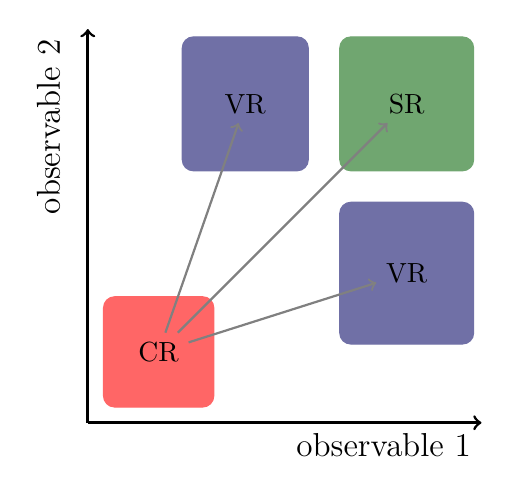
\begin{tikzpicture}

  \tikzstyle{region} = [rounded corners, fill]


  \draw[line width=1, ->] (0,0) -- (5,0) node[below left] {\large observable 1};
  \draw[line width=1, ->] (0,0) -- (0,5) node[left=0.5,rotate=90] {\large observable 2};

  \draw[region, red] (0.2,0.2) rectangle (1.6,1.6) node[midway,black] (CR) {CR};

  \draw[region, green] (3.2,3.2) rectangle (4.9,4.9) node[midway,black] (SR) {SR};

  \draw[region, blue] (3.2,1.0) rectangle (4.9,2.8) node[midway,black] (VR1) {VR};
  \draw[region, blue] (1.2,3.2) rectangle (2.8,4.9) node[midway,black] (VR2) {VR};

  \draw[->,gray, line width=0.8] (CR) -- (SR);
  \draw[->,gray, line width=0.8] (CR) -- (VR1);
  \draw[->,gray, line width=0.8] (CR) -- (VR2);

\end{tikzpicture}

  \caption{Esquema del diseño de las regiones de señal (SR), control (CR) y
    validación (VR) en términos de dos observables arbitrarios.}
  \label{fig:regions_sketch}
\end{figure}

Es importante que las CR, VR y SR sean estadísticamente independientes para
poder combinar la pdf que modela cada región en una pdf conjunta. Esto es
fundamental ya que al ajustar los parámetros de la función likelihood se deberá
hacer en un ajuste simultáneo. Esto es importante para poder compartir los
parámetros de los fondos y las incertezas sistemáticas entre las distintas
regiones de forma consistente.

%------------------------
% Extrapolacion CR -> SR
%------------------------
\section{Extrapolación y factores de transferencia}

Una de las suposiciones que se hizo en la sección anterior fue que las variables
cinemáticas que se usan para diferencias CR(s) y SR(s) están bien modeladas
después de haber ajustado la pdf total a los datos en las CR(s). Una vez que los
procesos de fondo dominantes son normalizados en las CR(s), las correspondientes
modificaciones en la pdf pueden ser extrapoladas a las VRs, las cuales son
utilizadas para verificar la validez de esta suposición inicial. Una vez que se
demuestra el acuerdo entre las predicciones del fondo normalizadas y los datos
observados en las VRs, las predicciones del fondo son extrapoladas a las SR(s),
y comparadas con los datos observados allí. Este proceso es llamado
\emph{unblinding} y es útil para validar la validez de las extrapolaciones y es
utilizado ampliamente en física para tener confianza en los métodos usados y
evitar utilizar predicciones prematuras y evitar un posible sesgo en el
resultado final.

En el procedimiento explicado anteriormente se utiliza de forma implícita los
denominados \emph{factores de transferencia}. Las predicciones de los fondo
normalizadas en el ajuste son:

\begin{align}
  N_p^{\text{est}}(\text{CR}) &= \mu_p \times \text{MC}_p (\text{CR})
  \\ N_p^{\text{est}}(\text{SR}) &= \mu_p \times \text{MC}_p (\text{SR})
\end{align}
%
donde $N_p^{\text{est}}(\text{CR})$ y $N_p^{\text{est}}(\text{SR})$ es el número
de eventos estimado para cada proceso de fondo $p$ y
$\text{MC}_p^{\text{est}}(\text{CR})$ y $\text{MC}_p^{\text{est}}(\text{SR})$ es
el número de eventos obtenido de las simulaciones MC. El factor $\mu_p$ es el
factor de normalización obtenido en el ajuste a datos.

%% En el ajuste, los valores estimados de fondo son tipicamente driven por la estadistica de las
%% CRs.

Definiendo $N_p^\text{fit}(\text{SR})$ como el valor ajustado en la CR, podemos
escribir de forma equivalente:

\begin{align}
  N_p^\text{est}(\text{SR}) &= \mu_p \times \text{MC}_p (\text{SR}) \nonumber
  \\ &\equiv N_p^\text{fit}(\text{CR}) \times \left[
    \frac{\text{MC}_p(\text{SR})}{\text{MC}_p(\text{CR})} \right]
\end{align}

El cociente que aparece dentro de los corchete es llamado \emph{factor de
  transferencia} (TF). Un aspecto importante de los TF es que que las incertezas
sistemáticas de los valores estimados de fondo pueden ser parcialmente
cancelados en la extrapolación. La incerteza total en el numero de eventos de
fondo en la SR es por lo tanto una combinación de las incertezas estadísticas en
las CRs y la incerteza sistemática residual de la extrapolación. Por esta razón
las CR suelen definirse con una selección un poco más relajada, para incrementar
la estadística, sin aumentar significativamente la incerteza en los TF, para
reducir las incertezas en la SR.

\section{Modelo}

La función likelihood conjunta contiene el parámetro de interés (la intensidad
de la señal), los factores de normalización para los procesos de fondo, y los
llamados parámetros nuisance que modelan el impacto de las incertezas
sistemáticas. Cada incerteza sistemática $i$ se describe con un parámetro
nuisance $\theta_i$ que interpola entre el valor nominal y las variaciones de
las incertezas sistemáticas. Es decir para las variaciones de las incertezas
sistemáticas $\pm \sigma$ tenemos $\theta_i = \pm 1$ y $\theta_i = 0$ para el
valor nominal.

La función likelihood general $L$ es el producto de los términos de Poisson del
número de eventos en la SR y las CR, y una distribución adicional que implementa
las condiciones en las incertezas sistemáticas. Puede escribirse como:

\begin{align}
  L(\bm{n}, \bm{\theta}^0| \mu_\text{sig}, \bm{\mu}_p, \btheta) &=
  \mathcal{P}_\text{SR} \, \times \, \mathcal{P}_\text{CR} \, \times \,
  \mathcal{C}_\text{syst} \nonumber \\
  &= \Pois(n|\lambda(\mu_\text{sig}, \bm{\mu}_p, \btheta)) \, \times \, \prod_{i \in \text{CR}}
  \Pois(n_i|\lambda_i(\mu_\text{sig}, \bm{\mu}_p, \btheta)) \times C_\text{syst} (\btheta^0, \btheta)
\end{align}
%
Los primeros dos factores ($\mathcal{P}_\text{SR}$ y $\mathcal{P}_\text{CR}$)
reflejan las distribuciones de Poisson de $n_i$, el número de eventos observado
en cada región. El valor esperado de la distribución de Poisson $\lambda_i$ son
funciones que dependen de las predicciones de señal y los distintos fondos $p$,
los parámetros nuisance que parametrizan las incertezas sistemáticas $\btheta$,
los factores de normalización para los procesos de fondo $\bm{\mu}_p$ y también
la intensidad de la señal $\mu_\text{sig}$. Para $\mu_\text{sig} = 0$ tenemos la
función likelihood para la hipótesis de solo-fondo y con $\mu_\text{sig} = 1$ el
valor esperado de señal para el valor nominal de modelo bajo consideración.

Las incertezas sistemáticas son incluidas usando la pdf
$C_\text{syst}(\btheta^0, \btheta)$, donde $\btheta^0$ son los valores centrales
de las medidas auxiliares alrededor de los cuales $\btheta$ puede variarse al
maximizar el likelihood.
El impacto
The impact of changes in nuisance parameters on the expectation values are
described completely by the functions predicting the amount of signal and background,
lambdaS and lambdai . Para parámetros nuisance


independientes $C_\text{syst}$ es simplemente el producto de las pdf
correspondientes a las mediciones auxiliares que describen cada una de las
incertezas sistemáticas, típicamente una distribución gaussiana $G$ con ancho
unidad,

\begin{equation}
  C_\text{syst} (\btheta^0, \btheta) = \prod_{j \in \text{S}} G(\theta_j^0 -
  \theta_j)
\end{equation}
%
donde S es el conjunto completo de las incertezas sistemáticas consideradas. Las
medidas auxiliares $\theta^0_j$ son típicamente fijadas a cero, pero pueden
variar cuando se generan los pseudo-experimentos.


\section{Ajustes}


\subsection{Bkg only fit}

El proposito  es estimar el fondo total en las SR y VR, sin hacer ninguna suposiscion del
modelo de senal. Solo se utilizan las muestras de fondo en el modelo. Las CR se asumen que eztan libres
de contaminacion de senal.  El ajuste solo se realiza en las CR y los procesos de fondo
dominantes se normalizan al numero de eventos observados en esas regiones.
Se utilizan la ec sin el termino de la SR.

Se comparten todos los parametros del ajuste, por lo tanto se usan para predecir
el numero de eventos de fondo en SR y VR.

Estas predicciones de fondo son independientes del numero de eventos observado en la SR (y VR)
ya que solo las CR se usan en el ajuste. Esto permite una comparasion no sesgada entre las
predicciones y el numero de evnetos observado en esas regiones.






----------------------------------

%% \section{Fit}

%% Analyses generally rely on external predictions for the various background and signal components
%% in the data to aid the interpretation of observations, where the signal component describes the
%% process of interest. In particle physics, simulations of known and hypothesized physics processes
%% are run through a detailed detector simulation, and are subsequently reconstructed with the same
%% algorithms as the data. In addition, background samples can be constructed using data-driven
%% methods. The simulated samples may depend on one or many model parameters, for example the
%% masses of hypothesized new particles such as foreseen by supersymmetry. It may be required, for
%% instance when signals are analyzed over a multi-dimensional space of model parameters, to sample
%% from a “grid” of potential signal scenarios, with each point on that grid corresponding to a unique
%% point in the multi-dimensional parameter space. If no excess is observed in the data, exclusion
%% limits may be set within this grid, excluding a subset of the tested parameter values.

%% \itodo{Podemos pensar a un experimento de conteo en el contexto de la eq 1 con
%%   $f(x) = 1$, reduciendoce solo al termino de Poisson}


%% \section{Medidas auxiliares}

%% Las medidas auxiliares o regiones de control puede ser utilizadas para reducir
%% el efecto de las incertezas sistemáticas. Las SR o CR no son fundamentalmente
%% distintas, en este lenguaje son dos canales distintos.

%% {\bf Common example: simple counting experiment with a background}

%% Desde el punto de vista frecuentista, el fondo desconocido en la región de se\~nal es un
%% parámetro nuisance, que llamamos $\nu_B$.

%% Si el numero de eventos de se\~nal es $\nu_S$ y el numero de eventos en la región de se\~nal
%% $n_\text{SR}$, podemos escribir el modelo $\Pois (n_\text{SR}|\nu_S+\nu_B)$.

%% Como $\nu_B$ es un parámetro libre, no podemos hacer ninguna inferencia acerca de $\nu_S$.
%% En general uno tiene una estimacion del fondo, que puede venir de una muestra de control
%% con $n_\text{CR}$ eventos.
%% Si la región de control no tiene contaminación de se\~nal y esta poblado con el mismo proceso
%% de fondo que la region de se\~nal, podemos escribir $\Pois(n_\text{CR}|\tau \nu_B)$, donde $n_\text{CR}$
%% es el numero de eventos en la región de control y $\tau$ es el factor utilizado para extrapolar
%% el fondo de la región de control a la región de se\~nal\todo{o al reves?}.

%% El modelo de probabilidad total puede escribirse
%% $\vec{f}_\text{sim}(n_\text{SR}, n_\text{CR}|\nu_S,\nu_B) = \Pois (n_\text{SR}|\nu_S+\nu_B) \cdot \Pois (n_\text{CR}|\tau\nu_B)$.

%% Basados solo en la CR, se puede estimar $\nu_B = n_\text{CR}/\tau$.  Intuitivamente
%% esta estimacion viene con una ``incerteza'' de $\sqrt{n_\text{CR}}/\tau$. El punto a
%% resaltar es que podemos usar mediciones auxiliares ($n_\text{CR}$) para describir la
%% incerteza en el parámetro nuisance $\nu_B$ estadísticamente. Creamos un modelo
%% estadístico que puede tratarse con un formalismo frecuentista. Se dice que las medidas
%% auxiliares \hl{constrain} los parámetros nuisance.

%% Total probability model:

%% \begin{equation}
%%   \vec{f}_\text{tot} (\mathcal{D}_\text{sim},\mathcal{G}|\alpha) = \prod_{c \in \text{canales}} \left[ \Pois(n_c|\nu_c{(\alpha)}) \prod_{e=1}^{n_c} f_c (x_{c,e}|\alpha) \right] \cdot \prod_{p \in S} f_p (a_p|\alpha_p)
%% \end{equation}

%% \subsection{Tratamiento de las incertezas sistematicas} \label{sec:fit_syst}

%% Treatment of the Systematic Uncertainties in the likelihood is described below. Gaussian PDFs are used
%% to model the systematic uncertainties, each having nominal values $\mu^{0}$ around which $\mu$ can be varied when
%% maximizing the likelihood. Theoretical and uncertainties on the background are taken into account as
%% well as detector uncertainties on the signal. Correlations between nuisance parameters can be treated
%% properly as 1) overall scale factors fully correlated across the different regions and the different components
%% (like luminosity), 2) scale factors fully correlated across the different regions but independent per component
%% (like theory uncertainties), and 3) fully uncorrelated variables (like Monte-Carlo statistical
%% errors) with one parameter per region. %The numbers of the uncertainties used as the fit inputs can be found in \Tab \ref{}.



%% \section{Herramientas para el análisis estadístico}

%% Para el analisis estadistico se utilizo el software \texttt{HistFitter} \cite{histfitter}
%% desarrollado dentro del grupo de SUSY en ATLAS, que es una interfaz para herramientas
%% como \texttt{RooFit}, \texttt{RooStats}\cite{Moneta:2010pm} y \texttt{HistFactory}
%% \cite{Cranmer:1456844} y ademas posee una serie de scripts que facilitan el analisis cuando este
%% es muy complejo.

\chapter{Simulaciones Monte Carlo}


\note{Mirar ``Perspective in SUSY II'' de Kane,
Capitulo 11}

\section{Generadores de eventos}

El eslabón entre la teoría (y fenomenología) de SUSY o cualquier otra teoría de
nueva física, y las observaciones experimentales en los detectores de los
colisionadores son los <<generadores de eventos>>. Dada una teoría de nueva
física, que en general predice la existencia de nuevas partículas y/o
interacciones, el generador de eventos permite calcular como esa teoría se
manifiesta en el experimento.

El primero paso para conectar SUSY con el experimento es comenzar con un modelo
particular de SUSY, y calcular el espectro de masas y acoplamientos de las
sparticulas. Existen varios programas que permiten calcula el espectro de masas:
Isasugra, Suspect, SoftSusy y Spheno. A partir de este modelo también es posible
calcular los anchos de decaimiento y tazas de decaimiento (BR) de todas las
sparticulas y los bosones de Higgs tanto $1 \to 2$ cuerpos y $1 \to 3$ cuerpos.

En este trabajo utilizamos el programa {\susyhit}\note{ref} que combina
{\suspect} junto {\sdecay} y {\hdecay} para calcular los BRs y anchos de
decaimiento. Algunos de estos modos de decaimientos son calculados a NLO en QCD.

Una vez que el espectro de masas y los decaimientos están calculados estos
pueden usarse como entrada en los generadores de eventos.

% SLHA
Para facilitar el intercambio de información entre distintos programas de SUSY
se propuso una seria de convenciones: SUSY Les Houches Accord (SLHA)\cite{SLHA}.
Este acuerdo permite usar la salida de los códigos que calculan el espectro de
masa y decaimientos como entrada en los generadores de eventos de una forma
consistente y sin ambigüedades.

%% %% En general estos modelos pueden
%% %% ser teorias efectivas
%% La teoria efectiva queda especificada adoptando la simetria de
%% gauge, the (super)field content y el Lagrangiano.
%% {\suspect} runs the 2-loop MSSM RGEs to determine weak scale
%% SUSY parameters in the mSUGRA, GMSB and AMSB models,
%% and in the pMSSM (a more general MSSM model). One-loop
%% sparticle mass corrections are included.
%% Some two loop corrections to Higgs masses are included.

\hl{agregar xs calculators}

\vsp

Los programas descriptos anteriormente permiten pasar de un modelo
de SUSY a las predicciones en la produccion de sparticulas y sus
anchos de decaimientos en estados finales de quarks, leptones, fotones
y gluones (y LSP en modelos donde se conserva paridad-R). Sin embargo
los quarks y gluones no pueden medirse directamente en los detectores.
Los detectores pueden medir trazas de particulas (cuasi)estables
cargadas y su momento en campos magnetics. Tambien pueden medir
depositos de enregia en los calorimetros .
Por lo tanto todavia hay un gap entre estos modelos y las senales
detectadas en los detectores. Los generadores de eventos permiten unir
estas dos cosas. Estos pueden producir una simulacion completa de los
eventos de dispersion esperados. El estado final de cualquier evento
de dispersion simulado esta compuesto por una lista de electrones,
muones, fotones y hadrones de vida media alta y su momento asociado
que puede ser medido en un experimento de colisiones.

Para un dado tipo de colisionador ($e^+e^-, pp, p\bar{p}, ...$) y una
dada energia de centro de masa, y un modelo, el generador de eventos
va a generar un conjunto eventos de pares de sparticulas de acuerdo
a su seccion eficaz. Estas sparticulas van a decaer (posiblemente
en en una cascada de varios pasos) en un estado final partonico,
de acuerdo a los BR fijados por el modelo. Este estado final partonico
es convertido es convertido en uno con particulas que puede ser detectadas
en el detector. Generando un gran numero de eventos de SUSY, se puede
simular los posibles estados finales que se esperada que un cierto
modelo produzca.

Existen varios generadoes que incorporan SUSY: Isajet, Pythia, Herwig, Sherpa, ....

La simulacion de eventos de dispersion en colisionadores hadronicos
puede descomponerse en varios pasos como se muestra en la figura [].

\begin{itemize}\itemsep0.2cm\parskip0.2cm
\item el calculo perturbativo del proceso de dispersion dura en el
  modelo partonico, y la convolucion con las funciones de distribucion
  partonica (PDFs)
\item la inclusion de los decaimientos en cascada de las sparticulas
\item implementacion de las lluvias de particulas pertubativamente
  para los estados de particulas con color inicial y final, y otras
  particulas con color que puedan ser producidas como decaimiento
  de otros objetos mas pesados,
\item implementacion del modelo de hadronizacion que describe la
  formacion de mesones y bariones a partir de los quarks y gluones.
  Tambien las particulas inetables deben decaer a hijas (cuasi)
  estables que son detectadas en el detector, con tasas y distribuciones
  que esten de acuerdo con los valores medidos o predichos.
\item Y finalmente, los remanentes de los haces inicilaes tienen que
  ser modelados para obtener una descripcion valida de la fisica
  en las regiones forward del detector.
\end{itemize}









\section{Herramientas para el calculo de SUSY}

\subsection{SUSY Spectrum Calculator}
\subsection{Sparticle Production and decay modes: production cross section, dacay widths and BF}
\subsection{Generadores de eventos: hard scattering, parton showers, cascade decays, hadronization}




















Las muestras de se\~nal de SUSY y de fondo del {\SM} fueron simuladas utilizando generadores MC
a $\sqrt{s}=8\tev$.
Todas las muestras fueron passed through either a GEANT4-based full simulation \cite{Geant4,AtlasSim}
or ATLFAST-II fast simulation \cite{Richter-Was:683751} of the ATLAS detector \cite{Geant4,AtlasSim},
and reconstructed with the same algorithms used for the data. An event-by-event reweighting is
applied to all MC samples to model the realistic machine conditions of the data sample
under study, by matching the simulated distribution of the number of interactions per bunch
crossing (pile-up) to the one observed in data.
The simulation details are summarized in {\Sec} \ref{sec:sig_samples} and \ref{sec:bkg_samples}.
Most of the MC backgrounds are, however, only used for comparison and cross checks.
The expected backgrounds in the selected sample is estimated, whenever possible,
from the data themselves. %(on average 5.6 interactions per bunch crossing).

\section{Se\~nal}\label{sec:sig_samples}

The present analysis is motivated by the bino-higgsino admixture neutralino decay signatures predicted by General Gauge Mediation (GGM) models,
namely a final-state signature that consists of a photon, jets, and high \MET. The event selection described in {\Sec} \ref{sec:event_selection},
has been designed to maximize the sensitivity to a small signal with this general topology. Any imposition of model-tailored selection cuts has been
avoided, trying to keep the analysis as model independent as possible. However, an interpretation in the framework of a specific model is unavoidable.
A grid of GGM signal points is simulated with a specific set of benchmark parameter values that covers the region in which signal can be established.
The sensitivity of the analysis is evaluated using this grid of points.

In this particular region of the GGM model space, the lightest neutralino is a mixture of bino and higgsino. The neutral wino is much heavier so it
does not contribute. Due to the Weinberg mixing angle in the Standard Model, the bino component of the lightest neutralino couples to both the photon and the Z.
The gluino is regarded as the only relevant coloured sparticle in order to set a conservative limit on the gluino mass. All squark soft masses are set to 2.5 TeV.
The other model parameters are set to M$_2$=2.5 \tev, $\tan\beta$=1.5 and $c\tau_{\mathrm{NLSP}} < 0.1$ mm. The latter assures the neutralino is decaying promptly
and is achieved by making the gravitino sufficiently light ($m_{\tilde{G}}=10^{-9}$ \gev). All trilinear coupling terms are set to zero and masses of sleptons
are set to 2.5 \tev. The Higgs boson is in the decoupling regime with $m_{A}$ = 2 \tev~ and $m_{h}$ = 126 \gev. The last follows the recently measured value
for the SM Higgs boson at the LHC \cite{ATLAS-CONF-2013-014,CMS-PAS-HIG-14-009}. In gauge mediated SUSY scenarios several mechanisms exist \cite{Craig:2011yk,Auzzi:2011eu,Csaki:2012fh,Larsen:2012rq,Craig:2012hc}
to generate a Higgs boson mass as high as this observed value, without changing the phenomenology of the models here considered. No significant effect on the mass spectrum
has been indeed observed when varying this value within a $\pm 10~$ \gev\ range.

\M{1} and $\mu$ determine the lightest neutralino mass, and are related in such a way that the branching ratios of the \ninoone\ are approximately constant,
resulting in ${\rm BR}(\ninoone \to \gam + \gravino) \approx 50\%$, ${\rm BR}(\ninoone \to Z + \gravino) \approx 49\%$ and ${\rm BR}(\ninoone \to h + \gravino) \approx 1\%$,
numbers which vary by $\pm 1\%$ throughout most of the grid ({\fig} \ref{fig:br_n1_x_grav}). For light neutralinos ($<200\gev$) the Higgs production is highly
suppressed and ${\rm BR}(\ninoone \to \gam + \gravino)$ starts falling up to 40\%. The value of $\mu$ must also be positive in order to disfavor the branching ratio
to the Higgs boson, which would lead to a signature already covered by a dedicated analysis in ATLAS \cite{Aad:2012jva}. Similarly, the branching ratio for
($\ninoone \to \gam + \gravino$) is such that maximizes the single photon final state. At larger values the diphoton topology starts to be favoured, which has been
extensively searched for in the past \cite{Aad2012519,Aad:2011kz}. This leaves $M_3$ and $\mu$ as the only two free parameters of the model, spanning the space
within $150\gev < m_{\ninoone} < 1250 \gev$ and $800\gev < m_{\gluino} < 1300 \gev$, with $m_{\ninoone} < m_{\gluino}$. The granularity of the simulation in each
dimension is shown in {\tab}\ \ref{tab:signal_pars}, with the resulting value for the gluino and neutralino masses.

The full mass spectrum, the gluino and neutralino branching ratios and decay widths are calculated from
these set of parameters using SUSPECT v2.41 \cite{Djouadi2007426}, SDECAY v1.3b \cite{Muhlleitner:2004mka}
and HDECAY v3.4 \cite{Djouadi:1997yw}, run as part of the SUSYHIT package v1.3 \cite{Djouadi:2006bz}.
An example of the mass spectrum in the configuration is shown in {\fig} \ref{fig:mass_spectra}, for one of
the signal grid points. The total decay branching ratios for \gluino-initiated \ninoone\ production are
shown in {\fig} \ref{fig:br_gl_n1}, for 2-body\footnote{only effectively, the gluino decays through a virtual
quark-squark loop in this case.} and 3-body gluino decays.
Simulated events were generated with HERWIG++ v2.5.2 \cite{Bahr:2008pv} for the 124 signal points in the
grid (5K per each), using the CTEQ6L1 \cite{Nadolsky:2008zw} parton density distributions. A generator level
filter requiring a photon with $p_{T}>100~$ \gev\ was applied to get higher statistics, specially at low neutralino
mass. The filter efficiency for all simulated points are shown in {\tab} \ref{tab:signal_filter_eff}.

Signal production cross sections and uncertainties were calculated using the SUSYSignalUncertainties package \cite{SUSYsigunc}. Cross sections
for the signal processes involving the production of gluino pairs are calculated to next-to-leading order (NLO)
in the strong coupling constant, adding the resummation of soft gluon emission at next-to-leading-logarithmic
accuracy (NLO+NLL) \cite{Beenakker:1996ch,Kulesza:2008jb,Kulesza:2009kq,Beenakker:2009ha,Beenakker:2011fu}.
The EWK $\tilde{\chi}\tilde{\chi}$ production cross sections are calculated to next-to-leading order in the strong coupling constant (NLO) using PROSPINO v2.1~\cite{Beenakker:1999xh}.
%are computed at NLO with Prospino v2.1 \cite{Beenakker:1996ed}.
The cross sections and uncertainties are tabulated in {\tab} \ref{tab:signal_xs_strong} and \ref{tab:signal_xs_ewk}, and shown in {\fig} \ref{fig:signal_xs_strong} and \ref{fig:signal_xs_ewk}, for the strong and EWK production respectively.
The total nominal cross section and the relative contribution of EWK produced processes are also shown in {\fig} \ref{fig:signal_xs_total}.
The total uncertainty is taken from an envelope of cross section predictions using different PDF
sets and factorisation and renormalisation scales, as described in \cite{Kramer:2012bx}.
More details of the uncertainties treatment are given in {\Sec} \ref{sec:syst_signal}. %The dependence of the cross section with $M_3$ is also shown in Fig. \ref{fig:signal_xs}.

All signal samples have been simulated with the faster, parametrized detector simulation ATLFAST-II \cite{Richter-Was:683751}. Derived datasets in the {\sc NTUP\_SUSY}
format are used throughout this analysis, with the configuration tag p1328.


\begin{figure}[ht!]
   \centering
   \includegraphics[width=0.4\textwidth]{figures/n1_gravgam}
   \includegraphics[width=0.4\textwidth]{figures/n1_gravz}\\
   \includegraphics[width=0.4\textwidth]{figures/n1_gravh}
   \caption{Branching ratios of the lightest neutralino (N1) decay. As expected in GGM models,
     the gravitino (as LSP) is always produced, in association with either a photon, a Z boson
     or a light Higgs boson, depending on the neutralino's nature. The grid parameters in this
     analysis have been chosen in order to keep the BR($\ninoone\to\gam\gravino)\sim50$\% across the whole phase space, maximizing the probability of the single photon final state. See text for more details.}
   \label{fig:br_n1_x_grav}
\end{figure}

\begin{table}[ht!]
  \centering
  \caption{ Model parameters of the GGM signal grid. $M_3$ and $\mu$ are regarded as the free parameters of the model. }
  \begin{tabular}{ccc || cccc}
    \hline
    \hline
    $M_3$ [\gev]& $m_{\gluino}$ [\gev]& &  & $\mu$ [\gev]& $M_1$ [\gev]& $m_{\ninoone}$ [\gev] \\
    \hline
    800 & 885.5   & & & 150  &  300  & 147.0  \tabularnewline
    850 & 931.7   & & & 175  &  270  & 168.3  \tabularnewline
    900 & 977.6   & & & 200  &  267  & 190.3  \tabularnewline
    950 & 1023.1  & & & 250  &  288  & 235.8  \tabularnewline
    1000 & 1068.3 & & & 350  &  365  & 332.4  \tabularnewline
    1050 & 1113.3 & & & 450  &  456  & 433.2  \tabularnewline
    1100 & 1157.9 & & & 550  &  551  & 535.6  \tabularnewline
    1150 & 1202.3 & & & 650  &  647  & 638.3  \tabularnewline
    1200 & 1246.4 & & & 750  &  745  & 742.0  \tabularnewline
    1250 & 1290.3 & & & 838  &  837  & 836.4  \tabularnewline
    1300 & 1333.9 & & & 850  &  845  & 846.7  \tabularnewline
    1350 & 1377.3 & & & 883  &  882  & 883.7  \tabularnewline
    1400 & 1420.5 & & & 928  &  926  & 930.2  \tabularnewline
    1450 & 1463.4 & & & 950  &  942  & 949.6  \tabularnewline
             &        & & & 973  &  970  & 976.6  \tabularnewline
             &        & & & 1017 &  1015 & 1023.4 \tabularnewline
             &        & & & 1050 &  1040 & 1053.0 \tabularnewline
             &        & & & 1062 &  1058 & 1068.9 \tabularnewline
             &        & & & 1106 &  1102 & 1114.8 \tabularnewline
             &        & & & 1149 &  1145 & 1160.0 \tabularnewline
             &        & & & 1150 &  1140 & 1157.5 \tabularnewline
             &        & & & 1250 &  1238 & 1260.6 \tabularnewline
    \hline
    \hline
  \end{tabular}
  \label{tab:signal_pars}
\end{table}

\begin{table}[ht]
  \centering
  \caption{Sección eficaz a  NLO+NLL para la producción fuerte de
    la grid de señal. La ultima columna es la incerteza teórica.
    Mas detalles se encuentran en la {\Sec} \ref{sec:syst_signal}.}
  \begin{tabular}{c|c|c}
    \hline
    \hline
    $M_3$ [\gev] & $\sigma$(NLO+NLL) [pb] & Incerteza Total Teorica [$\%$]\tabularnewline
    \hline
        800  &  0.06905 & 22.5  \\
        850  &  0.04492 & 23.8  \\
        900  &  0.02973 & 25.2  \\
        950  &  0.01983 & 26.5  \\
        1000 &  0.01341 & 27.7  \\
        1050 &  0.00910 & 29.0  \\
        1100 &  0.00628 & 30.4  \\
        1150 &  0.00432 & 32.0  \\
        1200 &  0.00301 & 33.7  \\
        1250 &  0.00210 & 35.2  \\
        1300 &  0.00148 & 36.7  \\
        1350 &  0.00105 & 38.2  \\
        1400 &  0.00074 & 39.8  \\
        1450 &  0.00053 & 41.5  \\
    \hline
    \hline
  \end{tabular}
  \label{tab:signal_xs_strong}
\end{table}

\begin{table}[ht]
  \centering
  \caption{Sección eficaz total a NLO para la producción EWK
    de la grid de señal. La ultima columna  es la incerteza
    teórica. Mas detalles se encuentran en la {\Sec} \ref{sec:syst_signal}.}
  \begin{tabular}{c|c|c}
    \hline
    \hline
    $\mu$ [\gev] & $\sigma$(NLO) [pb] & Total Theo. Uncertainty [$\%$]\tabularnewline
    \hline
    150  & 2.68 & 6.3  \\
    175  & 1.42 & 6.7  \\
    200  & 0.84 & 6.9   \\
    250  & 0.28 & 6.4     \\
    350  & 0.050 & 7.0    \\
    450  & 0.013 & 7.6    \\
    550  & 4.1e-03 & 8.0  \\
    650  & 1.4e-03 & 8.5   \\
    750  & 5.3e-04 & 8.9  \\
    850  & 2.1e-04 & 9.3  \\
    950  & 8.57e-05 & 10.3  \\
    1050  & 3.56e-05 & 11.0  \\
    1150  & 1.55e-05 & 13.3   \\
    1250  & 6.67e-06 & 16.9   \\
    \hline
    \hline
  \end{tabular}
  \label{tab:signal_xs_ewk}
\end{table}


\begin{table}[ht]
  \centering
  %\small
  \footnotesize
  \caption{Eficiencia del filtro a nivel generador [\%]
    para los puntos de señal simulados.}
  \begin{tabular}{c|ccccccccccccccccc}
    \hline
    \hline
%       &    \multicolumn{11}{c}{Filter efficiency [\%]} \\
%	\hline
     &   \multicolumn{14}{c}{ $M_3$ [\gev] } \\
    $\mu$ [\gev] &  800 & 850 & 900 & 950 & 1000 & 1050 & 1100 &1150 & 1200  & 1250 & 1300 & 1350 & 1400 & 1450 \\
    \hline
    150  &   39.54 &   39.8 &  41.9    &   42.6   &   43.0   &   44.2   &   45.5    &   46.3    &    47.1  &   48.3  &   49.1 &      &      &       \\
    175  &   44.55 &   44.6 &  46.5    &   47.5   &   47.8   &   48.9   &   50.3    &   51.4    &    51.5  &   52.4  &   53.3 &      &      &       \\
    200  &   47.66 &   48.4 &  50.1    &   50.6   &   52.0   &   52.8   &   53.8    &   55.0    &    55.0  &   56.2  &   56.0 &      &      &       \\
    250  &   55.09 &   56.0 &  56.1    &   57.1   &   56.7   &   58.0   &   58.9    &   59.5    &    60.5  &   60.7  &   61.2 & 62.1 & 62.2 &  63.9 \\
    350  &   65.82 &   66.1 &  64.6    &   65.8   &   66.4   &   66.7   &   66.5    &   67.7    &    67.4  &   67.6  &   67.8 & 68.0 & 69.2 &  68.4 \\
    450  &   71.29 &   71.4 &  71.4    &   71.8   &   72.1   &   72.5   &   72.0    &   72.6    &    72.1  &   72.5  &   73.4 & 72.9 & 72.2 &  73.4 \\
    550  &   73.08 &   72.5 &  73.3    &   73.7   &   74.6   &   74.3   &   75.0    &   74.8    &    74.2  &   74.7  &   75.6 & 75.7 & 74.9 &  75.3 \\
    650  &   69.78 &   72.0 &  73.2    &   74.1   &   75.6   &   76.2   &   75.9    &   75.8    &    77.0  &   77.0  &   76.2 & 76.7 & 77.1 &  76.6 \\
    750  &   47.69 &   60.2 &  66.9    &   70.4   &   73.4   &   74.0   &   75.9    &   76.5    &    77.1  &   77.3  &   76.3 & 77.9 & 77.2 &  77.0 \\
    838  &    9.0  &        &          &          &          &          &           &           &          &         &        &      &      &       \\
    883  &         &   9.1  &          &          &          &          &           &           &          &         &        &      &      &       \\
    850  &         &        &  34.2    &   50.7   &   60.1   &   66.4   &   70.4    &   73.5    &    73.6  &   75.4  &   76.6 & 77.1 & 78.2 &  76.8 \\
    928  &         &        &   9.4    &          &          &          &           &           &          &         &        &      &      &       \\
    950  &         &        &          &          &   25.4   &   41.4   &   54.0    &   62.2    &    66.8  &   70.9  &   75.2 & 75.9 & 78.1 &  77.2 \\
    973  &         &        &          &   10.0   &          &          &           &           &          &         &        &      &      &       \\
    1017 &         &        &          &          &   10.3   &          &           &           &          &         &        &      &      &       \\
    1050 &         &        &          &          &          &          &   19.2    &   31.6    &    45.2  &   56.8  &   62.7 & 68.9 & 73.1 &  75.6 \\
    1062 &         &        &          &          &          &   11.1   &           &           &          &         &        &      &      &       \\
    1106 &         &        &          &          &          &          &   11.7    &           &          &         &        &      &      &       \\
    1149 &         &        &          &          &          &          &           &   12.6    &          &         &        &      &      &       \\
    1150 &         &        &          &          &          &          &           &           &    16.1  &   24.9  &   36.9 & 49.0 &      &       \\
    1250 &         &        &          &          &          &          &           &           &          &         &   16.1 &      &      &       \\
    \hline
         \hline
  \end{tabular}
  \label{tab:signal_filter_eff}
\end{table}


%\begin{table}[ht]
%  \centering
%  \small
%  \begin{tabular}{|c|c|c|c|c|c|}
%    \hline
%    \hline
%	M3 [\gev] & $\sigma$(NLO+NLL) [\gev] & Uncertainty [$\%$] & k-factor & $m_{\neut}$ [\gev] & Filter efficiency [$\%$] \tabularnewline
%    \hline
%	\multirow{9}{*}{800} & \multirow{9}{*}{5.96 E-2} & \multirow{9}{*}{26.1} & \multirow{9}{*}{2.84} &  150 &  39.54 \\
%    \tiny
%	& & & & 175 & 44.55 \\
%	& & & & 200 & 47.66 \\
%	& & & & 250 & 55.09 \\
%	& & & & 350 & 65.82 \\
%	& & & & 450 & 71.29 \\
%	& & & & 550 & 73.08 \\
%	& & & & 650 & 69.78 \\
%	& & & & 750 & 47.69 \\
%	\hline
%	850 & 3.81 E-2 & 27.8 & 2.95 &  150 & 39.8 \tabularnewline
%	& & & & 175 & 44.6 \\
%	& & & & 200 &  48.4 \\
%	& & & & 250 &  56.0 \\
%	& & & & 350 &  66.1 \\
%	& & & & 450 &  71.4 \\
%	& & & & 550 &  72.5 \\
%	& & & & 650 &  72.0 \\
%	& & & & 750 &  60.2 \\
%	\hline
%	900 & 2.47 E-2 & 29.5 & 3.07 & 150 & 41.9 \tabularnewline
%	& & & & 175 &  46.5 \\
%	& & & & 200 &  50.1 \\
%	& & & & 250 &  56.1 \\
%	& & & & 350 &  64.6 \\
%	& & & & 450 &  71.4 \\
%	& & & & 550 &  73.3 \\
%	& & & & 650 &  73.2 \\
%	& & & & 750 &  66.9 \\
%	& & & & 850 &  34.2 \\
%	\hline
%	950 & 1.62 E-2 & 31.4 & 3.19 & 150 & 42.6 \tabularnewline
%	& & & & 175 &   47.5 \\
%	& & & & 200 &   50.6 \\
%	& & & & 250 &   57.1 \\
%	& & & & 350 &   65.8 \\
%	& & & & 450 &   71.8 \\
%	& & & & 550 &   73.7 \\
%	& & & & 650 &   74.1 \\
%	& & & & 750 &   70.4 \\
%	& & & & 850 &   50.7 \\
%	\hline
%	1000 & 1.08 E-2 & 33.6 & 3.33 & 150 & 43.0 \tabularnewline
%	& & & & 175 &   47.8 \\
%	& & & & 200 &   52.0 \\
%	& & & & 250 &    56.7 \\
%	& & & & 350 &    66.4 \\
%	& & & & 450 &    72.1 \\
%	& & & & 550 &    74.6 \\
%	& & & & 650 &    75.6 \\
%	& & & & 750 &    73.4 \\
%	& & & & 850 &    60.1 \\
%	& & & & 950 &    25.4 \\
%	\hline
%	1050 & 7.19 E-3 & 35.8 & 3.49 & 150 & 44.2 \tabularnewline
%	& & & & 175 &   48.9 \\
%	& & & & 200 &   52.8 \\
%	& & & & 250 &   58.0 \\
%	& & & & 350 &   66.7 \\
%	& & & & 450 &   72.5  \\
%	& & & & 550 &    74.3 \\
%	& & & & 650 &    76.2 \\
%	& & & & 750 &    74.0 \\
%	& & & & 850 &    66.4 \\
%	& & & & 950 &    41.4 \\
%	\hline
%	1100 & 4.87 E-3 & 37.8 & 3.66 & 150 & 45.5 \tabularnewline
%	& & & & 175 &   50.3 \\
%	& & & & 200 &   53.8 \\
%	& & & & 250 &   58.9 \\
%	& & & & 350 &   66.5 \\
%	& & & & 450 &   72.0 \\
%	& & & & 550 &   75.0 \\
%	& & & & 650 &   75.9 \\
%	& & & & 750 &   75.9 \\
%	& & & & 850 &   70.4 \\
%	& & & & 950 &   54.0 \\
%	& & & & 1050 &  19.2 \\
%	\hline
%	1150 & 3.29 E-3 & 40.0 & 3.85 &  150 & 46.3 \tabularnewline
%	& & & & 175 &   51.4 \\
%	& & & & 200 &   55.0 \\
%	& & & & 250 &   59.5 \\
%	& & & & 350 &   67.7 \\
%	& & & & 450 &   72.6 \\
%	& & & & 550 &   74.8 \\
%	& & & & 650 &   75.8 \\
%	& & & & 750 &   76.5 \\
%	& & & & 850 &   73.5 \\
%	& & & & 950 &   62.2 \\
%	& & & & 1050 &  31.6 \\
%	\hline
%	1200 & 2.24 E-3 & 42.3 & 4.05 &  150 & 47.1 \tabularnewline
%	& & & & 175 &   51.5 \\
%	& & & & 200 &   55.0 \\
%	& & & & 250 &   60.5 \\
%	& & & & 350 &   67.4 \\
%	& & & & 450 &   72.1 \\
%	& & & & 550 &   74.2 \\
%	& & & & 650 &   77.0 \\
%	& & & & 750 &   77.1 \\
%	& & & & 850 &   73.6 \\
%	& & & & 950 &   66.8 \\
%	& & & & 1050 &  45.2 \\
%	& & & & 1150 &  16.1 \\
%	\hline
%	1250 & 1.55 E-3 & 44.6 & 4.31 & 150 & 48.3 \tabularnewline
%	& & & & 175 &   52.4 \\
%	& & & & 200 &   56.2 \\
%	& & & & 250 &   60.7 \\
%	& & & & 350 &   67.6 \\
%	& & & & 450 &   72.5 \\
%	& & & & 550 &   74.7 \\
%	& & & & 650 &   77.0 \\
%	& & & & 750 &   77.3 \\
%	& & & & 850 &   75.4 \\
%	& & & & 950 &   70.9 \\
%	& & & & 1050 & 56.8 \\
%	& & & & 1150 & 24.9 \\
%	\hline
%	1300 & 1.07 E-3 & 46.9 & 4.56 & 150 & 49.1 \tabularnewline
%	& & & & 175 &   53.3 \\
%	& & & & 200 &   56.0 \\
%	& & & & 250 &   61.2 \\
%	& & & & 350 &   67.8 \\
%	& & & & 450 &   73.4 \\
%	& & & & 550 &   75.6 \\
%	& & & & 650 &   76.2 \\
%	& & & & 750 &   76.3 \\
%	& & & & 850 &   76.6 \\
%	& & & & 950 &   75.2 \\
%	& & & & 1050 & 62.7 \\
%	& & & & 1150 & 36.9 \\
%	& & & & 1250 & 16.1 \\
%    \hline
%    \hline
%  \end{tabular}
%  \caption{ The total NLO+NLL cross sections with uncertainties and K factors for GGM  signal points. The last column shows the efficiency of the generator level filter applied, to be considered for the final signal normalization.}
%  \label{tab:signal_xs}
%\end{table}

\begin{figure}[ht!]
   \centering
   \includegraphics[width=0.7\textwidth]{figures/figura} %%mass_spectrum_GGM.eps}
   \caption{Espectro de masas de un punto el grid de senal.
     Solo $M_3$ y $\mu$ son los parametros libres, en este caso
     $(M_3, \mu) = (800~\gev, 250~\gev)$. }
   \label{fig:mass_spectra}
\end{figure}

\begin{figure}[ht!] %  figure placement: here, top, bottom, or page
   \centering
   \includegraphics[width=0.32\textwidth]{figures/gl_n1g_full}
   \includegraphics[width=0.32\textwidth]{figures/gl_n1qq_full}
   \includegraphics[width=0.32\textwidth]{figures/gl_n1_full} \\
   \includegraphics[width=0.32\textwidth]{figures/gl_n2g_full}
   \includegraphics[width=0.32\textwidth]{figures/gl_n2qq_full}
   \includegraphics[width=0.32\textwidth]{figures/gl_n2_full} \\
   \includegraphics[width=0.32\textwidth]{figures/gl_n3g_full}
   \includegraphics[width=0.32\textwidth]{figures/gl_n3qq_full}
   \includegraphics[width=0.32\textwidth]{figures/gl_n3_full} \\
   \includegraphics[width=0.32\textwidth]{figures/gl_c1qq_full} \\

   \caption{Tasas de decaimiento para $\gluino \to \ninoone$,
     para todas las posibles cadenas de decaimiento permitidas en la grid
     de produccion fuerte. La mayoria de los graficos son la suma
     de deciamientos de 2 cuerpos (izquierda) y 3 cuerpos (centro).
     Para el decaimiento $\gluino \to \chinopm$), solo el decaimiento de
     tres cuerpos es posible.}
   \label{fig:br_gl_n1}
\end{figure}

\clearpage

%\begin{figure}[ht!]
%  \centering
%  \includegraphics[width=0.5\textwidth]{figures/GGM_xs_vs_M3}
%  \caption{Signal cross section as function of M3, calculated at NLO+NLL.}% See text for more details. }
%  \includegraphics[width=0.5\textwidth, angle=90]{figures/GGM_xs_vs_mgl}
%  \caption{Signal cross section as function of $m_{\gluino}$, calculated at NLO+NLL. \tosolve{UPDATE}}% See text for more details. }
%  \caption{Signal cross section for as function of $m_{\gluino}$, calculated at NLO+NLL. \tosolve{UPDATE}}% See text for more details. }
%  \label{fig:signal_xs_vs_M3}
%\end{figure}

%% \begin{figure}[htbp]
%% \centering
%% \subfloat[NLO+NLL cross section $pp \to \gluino\gluino$]{
%%   \includegraphics[width=0.49\textwidth]{figures/figura} %SigXsec_strong}
%%   \label{fig:signal_xs_strong}
%% }
%% \subfloat[NLO cross section $pp\to\susy{\chi}\susy{\chi}$]{
%%   \includegraphics[width= 0.49\textwidth]{figures/figura} %SigXsec_ewk}
%%   \label{fig:signal_xs_ewk}
%% }
%% \caption{Signal cross sections for the strong (\ref{fig:signal_xs_strong})
%%   and EWK (\ref{fig:signal_xs_ewk}) production grids.}
%% \label{fig:signal_xs}
%% \end{figure}

\begin{figure}[ht!]
  \centering
  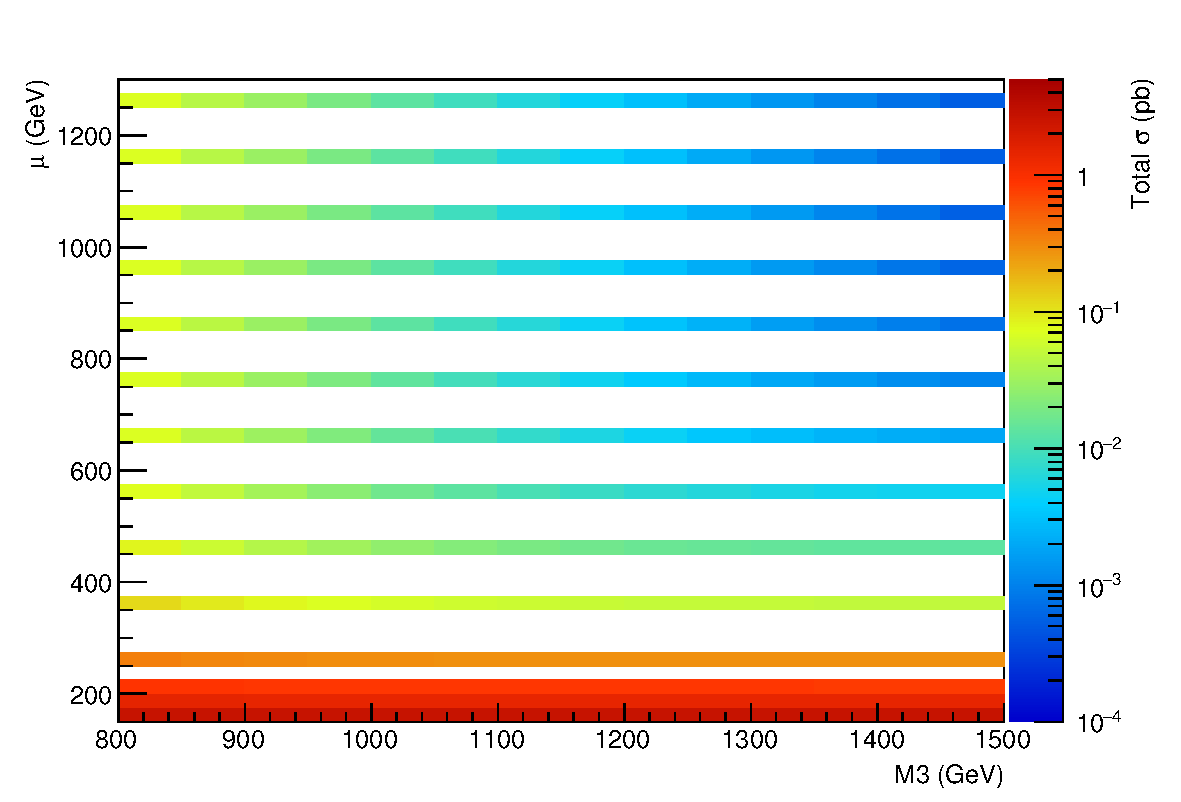
\includegraphics[width=0.49\textwidth]{figures/SigXsec_total}
  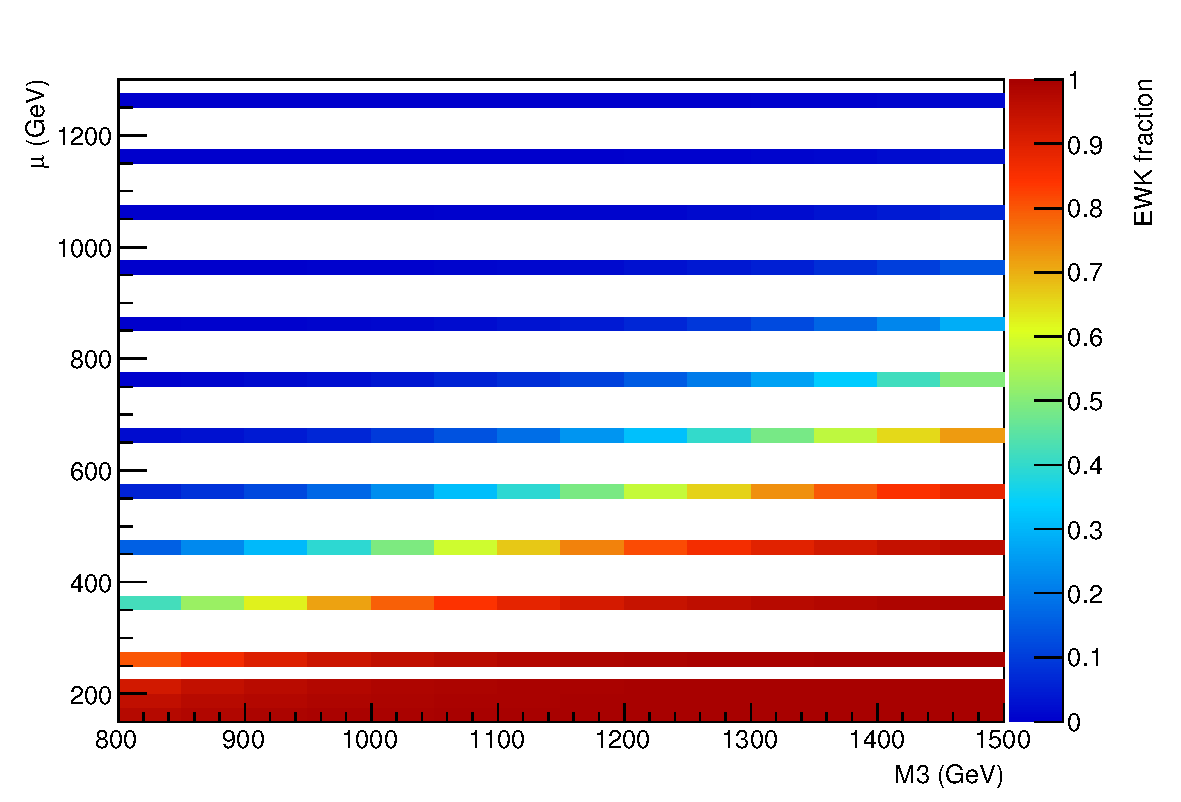
\includegraphics[width=0.49\textwidth]{figures/SigXsec_ewkFrac}
  \caption{Sección eficaz total (izquierda) y fracción relativa
    de producción EWK (derecha).}
  \label{fig:signal_xs_total}
\end{figure}

\section{Fondos del {\SM}}\label{sec:bkg_samples}

Existen muchos procesos del {\SM} que pueden aparentar
una señal de SUSY con fotones, jets y energía faltante.
Estos pueden dividirse en varias categorías:

\begin{itemize}
\item {\MET} real (EWK)
  \begin{itemize}
  \item $\gamma$ real
    \begin{itemize}
    \item $Z(\to\nu\nu)+\gamma$
    \item $W(\to\tau\nu)+\gamma$, hadronic $\tau$-decay
    \item $W(\to e\nu)+\gamma$, the e is not reconstructed
    \item $W(\to\mu\nu)+\gamma$ and $W(\to\tau\nu)+\gamma$, the $\mu / \tau$ is not reconstructed
    \item $t\bar{t}+\gamma$,  the e$/ \mu$ (when produced) is not reconstructed
    \end{itemize}

  \item Electron$/$Jet faking photon
    \begin{itemize}
    \item $W(\to l\nu)$+jets
    \item $Z(\to \nu\nu)+$jets
    \item $t\bar{t}$
    \item dibosons
    \end{itemize}
  \end{itemize}

\item {\MET} instrumental
  \begin{itemize}
  \item $\gamma$ real ($\gamma+$jets)
  \item $\gamma$ falso (multijet, $Z(\to ll)+$jets)
  \end{itemize}
\end{itemize}

Las muestras simuladas con MC utilizadas en este analisis se describen
a continuacion. Como se discutira en la {\Sec} \ref{sec:background_estimation},
la contaminacion de fotones mal dentificados provenientes de jets y electrones
es estimado con metodos basados en datos. Sin embargo, las muestras MC tambien
han sido consideradas en estos casos para los estudios de optimizacion y la
evaluacion de las incertezas sistematicas.

\subsection{W/Z$+\gamma$}

Se espera que la produccion de {\wgam} y {\zgam} sea un fondo importante
para esta busqueda. Ambas muestras fueron generadas usando el generador
de eventos {\sherpa} v1.4.1 \cite{SherpaGen}, con hasta 3 partones en el
ME+PS y usando las funciones de densidad partonica CT10.
La combinacion de los elementos de matriz con las lluvias partonicas
es realizada de acuerdo a un procedimiento mejorado CKKW \cite{Catani:2001cc,Krauss:2002up}.
Un filtro a nivel generados es aplicado requiriendo al menos un foton
con $\pt > 80(70) \gev$ en el estado final de las muestras de {\wgam} (\zgam).
%option1
%Only leptonic decays of the Z were considered, including its invisible decay Z$\to\nu\nu$. Additional samples of \wgamma events with some variation of the simulation settings were used to compute systematic uncertainties on the expected yields for this background. All \Vgamma samples are listed in {\tab} \ref{tab:bkg_wzgamma_samples}.
%option2
Todos los decaimientos leptonicos del boson $Z$ fueron considerados,
incluyendo el decaimiento invisible $Z\to\nu\nu$.
Tambien se tuvo en cuenta un muestra de $V(\to qq)+\gamma  (V=W,Z/\gamma*)$
debido a que cierta energia faltante real puede  ser producida en el caso
de heavy flavour decays.
%Their contribution had been found negligible in all regions here considered. \tosolve{CHECK!}
%

\begin{table}[ht!]
  \centering
  \caption{Muestras de W/Z$+\gamma$ utilizadas en este analisis.
    La seccion eficas a LO se especifica para cada modo de decaimiento,
    al igual que los factores $k$, y las eficiencias del filtro.
    La luminosidad integrada correspondiente a la estadistica total
    de cada muestra esta tambien presente.}
  %\includegraphics[width=1\textwidth]{figures/tabla}
  \begin{tabular}{ l | c | c | c | c }
    \hline
    \hline
    Proceso (ID) & $\sigma~[pb]$ & $k$ & Eficiencia & $L [fb^{-1}]$ \\
    \hline
    {\wenugam} {\sherpa} (126741) &  0.7193  &  1.0  &  1.0  &  695.16 \\
    {\wmunugam} {\sherpa}  (126744) &  0.7178  &  1.0  &  1.0  &  696.56 \\
    {\wtaunugam} {\sherpa}  (158727) &  0.7199  &  1.0  &  1.0  &  694.57 \\
    {\zeegam} {\sherpa}  (158728) &  0.1861  &  1.0  &  1.0  &  1069.53 \\
    {\zmumugam} {\sherpa}  (158729) &  0.1858  &  1.0  &  1.0  &  1076.71 \\
    {\ztautaugam} {\sherpa}  (158730) &  0.1858  &  1.0  &  1.0  &  1076.19 \\
    {\znunugam} {\sherpa}  (126022) &  0.7625  &  1.0  &  1.0  &  655.74 \\
  %%   % in case we use this in the end 'option2'
    {\vqqgam} {\sherpa}  (164438) &  6.756  &  1.0  &  1.0  &  89.0 \\
  %%   \hline
  %%   \hline
  %%   \multicolumn{5}{l}{Systematics variations} \\
  %%   \hline
  %%    \wenugam (fact. 0.25x) \sherpa (204733) &  0.7193  &  1.0  &  1.0  &  278.05 \\
  %%    \wenugam (fact. 4x) \sherpa (204734) &  0.7193  &  1.0  &  1.0  &  278.05 \\
  %%    \wenugam (renorm. 0.25x) \sherpa (204735) &  0.7193  &  1.0  &  1.0  &  278.05 \\
  %%    \wenugam (renorm. 4x) \sherpa (204736) &  0.7193  &  1.0  &  1.0  &  278.05 \\
  %%    \wenugam (ckkw 15) \sherpa (204731) &  0.7193  &  1.0  &  1.0  &  278.05 \\
  %%    \wenugam (ckkw 30) \sherpa (204732) &  0.7193  &  1.0  &  1.0  &  278.05 \\
  %%    \wmunugam (fact. 0.25x) \sherpa (204739) &  0.7193  &  1.0  &  1.0  &  278.63 \\
  %%    \wmunugam (fact. 4x) \sherpa (204740) &  0.7193  &  1.0  &  1.0  &  278.63 \\
  %%    \wmunugam (renorm. 0.25x) \sherpa (204741) &  0.7193  &  1.0  &  1.0  &  278.63 \\
  %%    \wmunugam (renorm. 4x) \sherpa (204742) &  0.7193  &  1.0  &  1.0  &  278.63 \\
  %%    \wmunugam (ckkw 15) \sherpa (204737) &  0.7193  &  1.0  &  1.0  &  278.63 \\
  %%    \wmunugam (ckkw 30) \sherpa (204738) &  0.7193  &  1.0  &  1.0  &  278.63 \\
  %%    \wtaunugam (fact. 0.25x) \sherpa (204745) &  0.7193  &  1.0  &  1.0  &  277.81 \\
  %%    \wtaunugam (fact. 4x) \sherpa (204746) &  0.7193  &  1.0  &  1.0  &  277.81 \\
  %%    \wtaunugam (renorm. 0.25x) \sherpa (204747) &  0.7193  &  1.0  &  1.0  &  277.81 \\
  %%    \wtaunugam (renorm. 4x) \sherpa (204748) &  0.7193  &  1.0  &  1.0  &  277.81 \\
  %%    \wtaunugam (ckkw 15) \sherpa (204743) &  0.7193  &  1.0  &  1.0  &  277.81 \\
  %%    \wtaunugam (ckkw 30) \sherpa (204744) &  0.7193  &  1.0  &  1.0  &  277.81 \\
    \hline
    \hline
  \end{tabular}
  \label{tab:bkg_wzgamma_samples}
\end{table}

\subsubsection{W/Z+jets} \label{mc_wzjets}

Se espera que la produccion de W$^{\pm}$ y bosones $Z$ en asociacion con jets
contribuya a esta busqueda, con los fotones provenientes de electrones y jets
mal identificados. Especialemente para los segundos, esta contaminacion no esta
bien descripta por el MC. Por esta razon se utilizan metodos basados en datos
para estimar su contirbucion en las diferentes regiones de senal y control, como
se describe en el Capítulo \ref{cap:fondos}. De igual maner varias muestras de MC
fueron consideradas para validar los metodos.

Como se describe en el Capítulo \ref{cap:seleccion} la seleccion de senal involucra
muchos jets en el estado final, es importante modelar los estados final multipartonicos
de forma adecuada. Con esto en mente, el generador de events {alpgen} (version 2.14)
fue utilizado, incluyendo los efectos EWK y QCD a LO para los procesos de interaccion
fuerte multipartonicos. La produccion de jets fue generada for up to five-parton
matrix elements. Este generados fue interfaceado con {\herwig} version 6.5.2
para la simulacion de las lluvias y los procesos de fragmentacion y con {\jimmy}
para la simulacion de los eventos subyacentes. Las funciones de densidad partonica
utilizadas fueron las CTEQ6L1. La normalizacion a la luminosidad integrada acumulada
fue hecha escalenado la seccion eficas mostrada en la {\tab} \ref{tab:bkg_wzjets_samples}
usando calculos QCD a NNLO de el programa FEWZ \cite{Anastasiou:2003ds}.
En cada caso los mismos factores de normalizacion fueron aplicados a los elementos
de matriz de {\alpgen}.
%%applied for all \alpgen matrix element parton multiplicities.
Finalmente, se realiza la remocion de eventos para evitar el conteo doble de eventos
que ya fueron tenidos en cuenta por las muestras de Z$\gamma$ y W$\gamma$.
Para esto, los eventos de $W(Z)+\text{jets}$ con fotones con $\pt > 80(70)\gev$
y $\Delta{\rm R}(e/\mu/\tau/$light-quarks$, \gamma) > 0.1$ fueron removidos
de las muestras.

\begin{table}[ht!]
  \centering
  \caption{Muestras de $W/Z+\text{jets}$ utilizadas en este analisis.
    La seccion eficas a LO para cada modo de decaimiento, los factores $k$
    (para la normalizacion NLO) y las eficiencias del filtro son reportadas,
    asi como tabine la luminosidad integrada correspondiente a la estadistica
    total de cada muestra.}
  \begin{tabular}{ l | c | c | c | c }
    \hline
    \hline
    Proceso (ID) & $\sigma~[pb]$ & k-factor & filter eff. & $\int{\mathcal{L}dt}~[fb^{-1}]$ \\
    \hline
    \zeenj{0}  \alpgen+\pythia (117650) & 718.89 & 1.18 & 1 & 7.80 \\
%    \zeenj{1}  \alpgen+\pythia (117651) & 175.60 & 1.18 & 1 & 6.42 \\
%    \zeenj{2}  \alpgen+\pythia (117652) & 58.846 & 1.18 & 1 & 5.83 \\
%    \zeenj{3}  \alpgen+\pythia (117653) & 15.56   & 1.18 & 1 & 5.99 \\
%    \zeenj{4}  \alpgen+\pythia (117654) & 3.9322 & 1.18 & 1 & 6.47 \\
%    \zeenj{5}  \alpgen+\pythia (117655) & 1.1994 & 1.18 & 1 & 7.07 \\
%    \zmmnj{0}  \alpgen+\pythia (117660) & 718.89 & 1.18 & 1 & 7.79 \\
%    \zmmnj{1}  \alpgen+\pythia (117661) & 175.81 & 1.18 & 1 & 6.43 \\
%    \zmmnj{2}  \alpgen+\pythia (117662) & 58.805 & 1.18 & 1 & 5.84 \\
%    \zmmnj{3}  \alpgen+\pythia (117663) & 15.589 & 1.18 & 1 & 5.98 \\
%    \zmmnj{4}  \alpgen+\pythia (117664) & 3.9072 & 1.18 & 1 & 6.51 \\
%    \zmmnj{5}  \alpgen+\pythia (117665) & 1.1933 & 1.18 & 1 & 7.10 \\
%    \zttnj{0} \alpgen+\pythia (117670) & 718.85 & 1.18 & 1 & 7.80 \\
%    \zttnj{1} \alpgen+\pythia (117671) & 175.83 & 1.18 & 1 & 6.43 \\
%    \zttnj{2} \alpgen+\pythia (117672) & 58.630 & 1.18 & 1 & 5.85 \\
%    \zttnj{3} \alpgen+\pythia (117673) & 15.508 & 1.18 & 1 & 5.96 \\
%    \zttnj{4} \alpgen+\pythia (117674) & 3.9526 & 1.18 & 1 & 6.43 \\
%    \zttnj{5} \alpgen+\pythia (117675) & 1.1805 & 1.18 & 1 & 7.18 \\
    \zeenj{0}  \alpgen+\jimmy (107650) & 711.77 & 1.23 & 1 & 7.548 \\
    \zeenj{1}  \alpgen+\jimmy (107651) & 155.17 & 1.23 & 1 & 6.994 \\
    \zeenj{2}  \alpgen+\jimmy (107652) & 48.745 & 1.23 & 1 & 6.746 \\
    \zeenj{3}  \alpgen+\jimmy (107653) & 14.225 & 1.23 & 1 & 6.286 \\
    \zeenj{4}  \alpgen+\jimmy (107654) & 3.7595 & 1.23 & 1 & 6.487 \\
    \zeenj{5}  \alpgen+\jimmy (107655) & 1.0945 & 1.23 & 1 & 7.428 \\
    \zmmnj{0}  \alpgen+\jimmy (107660) & 712.11 & 1.23 & 1 & 7.557 \\
    \zmmnj{1}  \alpgen+\jimmy (107661) & 154.77 & 1.23 & 1 & 7.011 \\
    \zmmnj{2}  \alpgen+\jimmy (107662) & 48.912 & 1.23 & 1 & 6.731 \\
    \zmmnj{3}  \alpgen+\jimmy (107663) & 14.226 & 1.23 & 1 & 6.286 \\
    \zmmnj{4}  \alpgen+\jimmy (107664) & 3.7838 & 1.23 & 1 & 6.445 \\
    \zmmnj{5}  \alpgen+\jimmy (107665) & 1.1148 & 1.23 & 1 & 7.292 \\
    \zttnj{0} \alpgen+\jimmy (107670) & 711.81 & 1.23 & 1 &  7.560 \\
    \zttnj{1} \alpgen+\jimmy (107671) & 155.13 & 1.23 & 1 &  6.996 \\
    \zttnj{2} \alpgen+\jimmy (107672) & 48.804 & 1.23 & 1 &  6.746 \\
    \zttnj{3} \alpgen+\jimmy (107673) & 14.160 & 1.23 & 1 &  6.315 \\
    \zttnj{4} \alpgen+\jimmy (107674) & 3.7744 & 1.23 & 1 &  6.462 \\
    \zttnj{5} \alpgen+\jimmy (107675) & 1.1163 & 1.23 & 1 &  7.283 \\
    \hline
    \hline
    \wenunj{0}  \alpgen+\jimmy (107680) &8037.10   & 1.186 & 1 & 0.362 \\
    \wenunj{1}  \alpgen+\jimmy (107681) &1579.20   & 1.186 & 1 & 1.334 \\
    \wenunj{2}  \alpgen+\jimmy (107682) &477.20     & 1.186 & 1 & 6.661 \\
    \wenunj{3}  \alpgen+\jimmy (107683) &133.93     & 1.186 & 1 & 6.358 \\
    \wenunj{4}  \alpgen+\jimmy (107684) &35.62       & 1.186 & 1 &  5.917\\
    \wenunj{5}  \alpgen+\jimmy (107685) &10.55       & 1.186 & 1 &  5.592\\
    \wmnunj{0}  \alpgen+\jimmy (107690) &8040.00 & 1.186 & 1 &  0.363\\
    \wmnunj{1}  \alpgen+\jimmy (107691) &1580.30 & 1.186 & 1 &  1.333\\
    \wmnunj{2}  \alpgen+\jimmy (107692) &477.50   & 1.186 & 1 &  6.656\\
    \wmnunj{3}  \alpgen+\jimmy (107693) &133.94   & 1.186 & 1 &  6.357\\
    \wmnunj{4}  \alpgen+\jimmy (107694) &35.64      & 1.186 & 1 &  6.033\\
    \wmnunj{5}  \alpgen+\jimmy (107695) &10.57      & 1.186 & 1 &  1.595\\
    \wtnunj{0} \alpgen+\jimmy (107700)    &8035.80  & 1.186 & 1 & 0.353 \\
    \wtnunj{1} \alpgen+\jimmy (107701)    &1579.80  & 1.186 & 1 & 1.307 \\
    \wtnunj{2} \alpgen+\jimmy (107702)    &477.55    & 1.186 & 1 &  6.567\\
    \wtnunj{3} \alpgen+\jimmy (107703)    &133.79    & 1.186 & 1 &  6.365\\
    \wtnunj{4} \alpgen+\jimmy (107704)    &35.58      & 1.186 & 1 &  5.921\\
    \wtnunj{5} \alpgen+\jimmy (107705)    &10.54      & 1.186 & 1 &  5.199\\
    \hline
    \hline
  \end{tabular}
  \label{tab:bkg_wzjets_samples}
\end{table}


\subsubsection{Top pair ($+\gam$) production}\label{sec:mcttbargam}

Another important background to this analysis is \ttgam. This MC sample was generated using the
{\madgraph} \cite{Alwall:2007st} MC generator and the CTEQ6L1 PDF. %No fully hadronic \ttbar\ was included.
  {\pythiasix} \cite{pythia} was used for parton showering, fragmentation and underlying event
simulation. Additional photon radiation was added with
{\photos} \cite{photos}, and tau leptons were decayed with
{\tauola} \cite{tauola}. The truth-level photons were required to have
$\pt > 80 \gev$. To avoid kinematic effects introduced by the filter, the photon \pt\ cut on the reconstructed sample was raised to 95 \gev.
A $k$-factor of $1.9 \pm 0.4$ is used \cite{Melnikov:2011ta, tth}. %This was calculated by
%the theorists with the particular generator-level cuts used to                                                                                                                     %generate this MC sample.

Simulation details are given in {\tab} \ref{tab:bkg_ttbar_samples}. The MC samples with IDs 202332--202337 are truth-only systematic variation samples, used to estimate systematic
uncertainties as explained in {\Sec} \ref{sec:syst_ttbargamma}.


% NOT ANYMORE , but explained later why
%As described in {\sec} \ref{}, the normalization of this sample was extracted together with that for %W$+\gamma$ events by fitting
%simultaneously the two MC to data in specifically designed control regions.

%More information can be found in
%Ref.~\cite{ttbargammaSupport}.

La produccion de {\ttbar}, donde los electrones o los jets
son mal identificados como fotones es una fuente de fondo que
vale la pena considerar.

%% Although both fakes contamination were estimated from the data, simulated events were used at the  optimization stage
%% and for cross checks of the data-driven methods. The MC sample was generated using the
%% {\powheg} \cite{Nason:2004rx,Frixione:2007vw,Alioli:2010xd} generator, with the parton showering and fragmentation done in \pythia.
%% The new Perugia 2011C tune \footnote{see some details at \url{https://twiki.cern.ch/twiki/bin/viewauth/AtlasProtected/P2011C}.} was used for the underlying event,
%%  with the CTEQ6L1 LO* set of PDFs. Additional photon radiation was added with {\photos} \cite{photos}.
%% Overlap removal is performed to prevent double-counting the phase-space
%% covered by the {\ttgam} MC sample. Events with truth prompt photons with
%% $\pt > 95 \gev$ and $\Delta{\rm R}(e/\mu/\tau/g/$light-quarks$, \gamma) > 0.1$ are removed from the \ttbar\ sample.


%% ttbar normalization??

%The nominal normalization of this sample is based on a cross section
%calculated at approximate NNLO in QCD using Hathor
%1.2~\cite{Aliev:2010zk} using the MSTW2008 \unit[90]{\%} NNLO PDF
%sets~\cite{MSTW2008} and incorporating PDF+$\alpha_S$ uncertainties
%according to the MSTW prescription~\cite{Martin:2009bu}. The value is
%cross checked with the NLO+NNLL calculation of Cacciari et
%al.~\cite{Cacciari:2011hy} as implemented in Top++
%1.0~\cite{Czakon:2011xx}. An uncertainty of \unit[11.0]{\%} is assigned
%to the NNLO cross section (which incorporates the mass uncertainty).
%


\begin{table}[ht!]
  \centering
  \caption{\ttgam\ samples used for the analysis. The LO cross-section for specified decay mode, k-factors (for NLO normalisation) and filter efficiencies are reported. The integrated luminosities corresponding to the total statistics in each sample are also given. The bottom group of samples was used to study systematic uncertainties.}
  \includegraphics[width=1\textwidth]{figures/tabla}
  %% \begin{tabular}{ l | c | c | c | c }
  %%   \hline
  %%   \hline
  %%   Process (ID) & $\sigma~[pb]$ & k-factor & filter eff. & $\int{\mathcal{L}dt}~[fb^{-1}]$ \\
  %%   \hline
  %%   \hline
  %%   \ttbar\ \powheg+\pythia (117050)  & 253.00 & 1 & 0.543 & 580 \\
  %%   \hline
  %%   %    \ttbargam noAllHad \madgraph (164439) & 0.092363 & 1.9 & 1 & 1139.7 \\
  %%   \ttbargam\ noAllHad \madgraph (177998) & 0.09873 & 1.9 & 1 & 1066.2 \\
  %%   \ttbargam\ AllHad \madgraph (174382) & 0.068599 & 1.9 & 1 & 1534.5 \\
  %%   \hline
  %%   \hline
  %%   \multicolumn{5}{l}{Systematics variations} \\
  %%   \hline
  %%   \ttbargam\ noAllHad (scaleUP) \madgraph (202332) & 0.09873 & 1.9 & 1 & 1066.2 \\
  %%   \ttbargam\ noAllHad (scaleDN) \madgraph (202333) & 0.09873 & 1.9 & 1 & 1066.2 \\
  %%   \ttbargam\ noAllHad (alpsUP) \madgraph (202334) & 0.09873 & 1.9 & 1 & 1066.2 \\
  %%   \ttbargam\ noAllHad (alpsDN) \madgraph (202335) & 0.09873 & 1.9 & 1 & 1066.2 \\
  %%   \ttbargam\ noAllHad (moreFSR) \madgraph (202336) & 0.09873 & 1.9 & 1 & 1066.2 \\
  %%   \ttbargam\ noAllHad (lessFSR) \madgraph (202337) & 0.09873 & 1.9 & 1 & 1066.2 \\
  %%   \hline
  %%   \hline
  %% \end{tabular}
  \label{tab:bkg_ttbar_samples}
\end{table}

\subsubsection{Single top (+ $\gamma$) production}

Single top with an associated photon samples were produced using
Whizard 2.1.1 \cite{whizard, whizard2}, with 4-flavor /5-flavor
matching provided using Hoppet~\cite{hoppet}.\footnote{Thanks to
Fabian Bach for providing an early version of the matching, which
will be standard in Whizard 2.2.0.} The extra photon could be in
either the single top production or the subsequent decays. Production
and decay, however, was treated separately, so interference effects
are ignored. {\pythia} \cite{pythia} was used for parton showering and
fragmentation. Additional photon radiation was added with
{\photos} \cite{photos}, and tau leptons were decayed with
{\tauola} \cite{tauola}.

%We used sample IDs 202621 and 202622 for \tchangamma production, and
%sample IDs 202623--202631 for \tWgamma production.

\begin{table}[ht!]
  \centering
  \caption{Single top and \tgam\ samples used for the analysis. The NNLO cross-section, filter efficiencies and the integrated luminosities corresponding to the total statistics in each sample are also given.}
  \includegraphics[width=1\textwidth]{figures/tabla}
  %% \begin{tabular}{ l | c | c | c }
  %%   \hline
  %%   \hline
  %%   Process (ID) & $\sigma~[pb]$ & filter eff. & $\int{\mathcal{L}dt}~[fb^{-1}]$ \\
  %%   \hline
  %%   t-channel \acermc (110101)  & 28.4 & 1 & 271 \\
  %%   Wt        \powheg (110140)  & 22.4 & 1 & 892 \\
  %%   s-channel \powheg (110119)  & 1.82 & 1 & 3299 \\
  %%   \hline
  %%   \hline
  %%   \tgam (t-channel) \wizhard+\pythia (202621)  & 0.187298 & 0.121980 & 4810 \\
  %%   \tgam (t-channel) \wizhard+\pythia (202622)  & 0.313866 & 0.012927 & 4930 \\
  %%   \hline
  %%   \twgam (dilep.) \wizhard+\pythia (202623)  & 0.012915  & 0.164370 & 4710 \\
  %%   \twgam (dilep. tDec) \wizhard+\pythia (202624)  & 0.014538  & 0.028748 & 12000 \\
  %%   \twgam (dilep. WDec) \wizhard+\pythia (202625)  & 0.010405  & 0.075489 & 6370 \\
  %%   \twgam (tlepWhad) \wizhard+\pythia (202626)  & 0.025825 & 0.162440 & 4770 \\
  %%   \twgam (tlepWhad tDec) \wizhard+\pythia (202627)  & 0.029084  & 0.027609 & 6230 \\
  %%   \twgam (tlepWhad WDec) \wizhard+\pythia (202628)  & 0.011594  & 0.064709 & 6660 \\
  %%   \twgam (thadWlep) \wizhard+\pythia (202629)  & 0.025817 & 0.161780 & 4790 \\
  %%   \twgam (thadWlep tDec) \wizhard+\pythia (202630)  & 0.020127  & 0.041977 & 5920 \\
  %%   \twgam (thadWlep WDec) \wizhard+\pythia (202631)  & 0.020788  & 0.075740 & 3180 \\
  %%   \hline
  %%   \hline
  %% \end{tabular}
  \label{tab:bkg_st_samples}
\end{table}

The single top process is a small background for this analysis, mostly
important for the control and validation regions. $Wt$ production (ID 110140) was generated using the \powheg, including full next-to-leading order QCD
corrections. Parton showering and fragmentation were simulated by
\pythia with the P2011C tune. The CT10 next-to-leading-order parton
set is used for the matrix element, the parton shower and the
underlying event. The samples were scaled to the cross section
calculated in \cite{Kidonakis:2010ux}. For $t$-channel
production, the MC samples with sample ID 110101 were used, with the
$W$ boson decaying leptonically. These were generated with
\acermc \cite{acer}, with parton showering and fragmentation performed
by {\pythia} with the P2011C tune and CTEQ6L1 PDF set.  The samples were
scaled to the cross section calculated by \cite{Kidonakis:2011wy}.
Single top produced by $s$-channel was not used because it was found
to be negligible.

Overlap between the single top and single top $\gamma$ samples has been removed.

\subsubsection{Direct $\gamma+$jets and QCD multijet}

%The QCD background is one of the main source of background in this analysis, particularly prompt photon events. The QCD contamination is in all cases a result of pathological events (jet faking a photon, badly reconstructed jet or photon making high \MET) for which the simulation is not reliable.
%For this reason this background is computed with a data driven approach, as explained in {\sec} \ref{sec:jetsmearing}. Several MC simulations are used anyways for consistency checks and to assess systematic uncertainties.

The QCD contamination is in all cases a result of pathological events
(jet faking a photon, badly reconstructed jet or photon making high \MET).
However, it is not expected to be a dominant source of background in the
phase space explored in this analysis. The contribution from events with
jets faking a photon is estimated with the data driven described in
{\Sec} \ref{sec:jetfakes}. The QCD multijet samples listed in {\tab}
\ref{tab:bkg_qcd_samples} were used for optimisation and preliminar
sensitivity studies. Prompt photon production was simulated with
with {\sherpa} v1.4.1 \cite{SherpaGen}, with up to four partons in the ME+PS
and using the CT10 set of parton density functions. The inclusive spectrum
is sliced in ranges of photon \pt\ to optimise the event generation.
Alternative samples were used to asses systematics uncertainties and
cross checks, generated with {\pythiaeight} (using CTEQ6L1) and {\alpgen}
v2.14 (with same config as V$+$jets events described in {\Sec} \ref{mc_wzjets}).
Further details are given in {\tab} \ref{tab:bkg_qcd_samples}.

\begin{table}[ht!]
  \centering
  \caption{Muestras de QCD {\gjet} y multijet utilizadas en este analisis.
    La seccion eficas a LO para cada modo de decaimiento,
    y las eficiencias del filtro son reportadas,
    asi como tabine la luminosidad integrada correspondiente a la estadistica
    total de cada muestra.}

  %% \includegraphics[width=1\textwidth]{figures/tabla}

   \begin{tabular}{ l | c | c | c }
    \hline
    \hline
    Process (ID) & $\sigma~[pb]$ & filter eff. & $\int{\mathcal{L}dt}~[fb^{-1}]$ \\
    \hline
    {\gjet} ($\pt>70\gev$) {\sherpa}  ( 113715 ) &  2153.0  &  1.0  &  1.160 \\
    {\gjet} ($\pt>140\gev$) {\sherpa} ( 113716 ) &  137.85  &  1.0  &  10.881 \\
    {\gjet} ($\pt>280\gev$) {\sherpa}  ( 113717 ) &  5.963  &  1.0  &  167.657 \\
    {\gjet} ($\pt>500\gev$) {\sherpa}  ( 126731 ) &  0.276  &  1.0  &  3617.291 \\
    {\gjet} ($\pt>800\gev$) {\sherpa}  ( 126955 ) &  0.0133  &  1.0  &  7492.807 \\
    {\gjet} ($\pt>1000\gev$) {\sherpa}  ( 126956 ) &  0.00238  &  1.0  &  41980.269 \\
    \hline

    \hline
  \gjet\ ($\pt>70\gev$)   \pythiaeight ( 129172 ) &  3425000  &  $5.7 \times 10^{-4}$  &  1535.4  \\
  \gjet\ ($\pt>140\gev$) \pythiaeight ( 129173 ) &  122170  &  $9.7 \times 10^{-4}$  &  8449.2 \\
  \gjet\ ($\pt>280\gev$) \pythiaeight ( 129174 ) &  3348.7  &  $1.45 \times 10^{-3}$  &  206559.7 \\
  \gjet\ ($\pt>500\gev$) \pythiaeight ( 129175 ) &  115.63  &  $1.8 \times 10^{-3}$  &  4789097.0\\
    \hline

% \gjetnj{1} ($\ptgam>35\gev) \alpgen+\jimmy  ( 156841 ) &  9554.200195  &  1.0  &  0.00890 \\
 \gjetnj{1} ($\pt>70\gev$) \alpgen+\jimmy  ( 156843 ) &  577.480  &  1.0  &  0.147 \\
 \gjetnj{1} ($\pt>140\gev$) \alpgen+\jimmy  ( 156839 ) &  26.198  &  1.0  &  3.626 \\
 \gjetnj{1} ($\pt>280\gev$) \alpgen+\jimmy  ( 156840 ) &  0.83119  &  1.0  &  30.077 \\
 \gjetnj{1} ($\pt>500\gev$) \alpgen+\jimmy  ( 156842 ) &  0.029141  &  1.0  &  343.159 \\

% \gjetnj{2} ($\ptgam>35\gev$) \alpgen+\jimmy  ( 156846 ) &  4515.0  &  1.0  &  0.00886 \\
 \gjetnj{2} ($\pt>70\gev$) \alpgen+\jimmy  ( 156848 ) &  571.870  &  1.0  &  0.175 \\
 \gjetnj{2} ($\pt>140\gev$) \alpgen+\jimmy  ( 156844 ) &  38.671001  &  1.0  &  3.879 \\
 \gjetnj{2} ($\pt>280\gev$) \alpgen+\jimmy  ( 156845 ) &  1.6811  &  1.0  &  29.741 \\
 \gjetnj{2} ($\pt>500\gev$) \alpgen+\jimmy  ( 156847 ) &  0.075517  &  1.0  &  264.841 \\

% \gjetnj{3} ($\ptgam>35\gev$) \alpgen+\jimmy  ( 156851 ) &  1717.0  &  1.0  &  0.00874 \\
 \gjetnj{3} ($\pt>70\gev$) \alpgen+\jimmy  ( 156853 ) &  306.10  &  1.0  &  0.049\\
 \gjetnj{3} ($\pt>140\gev$) \alpgen+\jimmy  ( 156849 ) &  28.57  &  1.0  &  5.250 \\
 \gjetnj{3} ($\pt>280\gev$) \alpgen+\jimmy  ( 156850 ) &  1.538  &  1.0  &  32.503 \\
 \gjetnj{3} ($\pt>500\gev$) \alpgen+\jimmy  ( 156852 ) &  0.077073  &  1.0  &  77.822 \\

% \gjetnj{4} ($\ptgam>35\gev$) \alpgen+\jimmy  ( 156856 ) &  513.940002  &  1.0  &  0.00778 \\
 \gjetnj{4} ($\pt>70\gev$) \alpgen+\jimmy  ( 156858 ) &  115.850  &  1.0  &  0.216 \\
 \gjetnj{4} ($\pt>140\gev$) \alpgen+\jimmy  ( 156854 ) &  14.216  &  1.0  &  11.951 \\
 \gjetnj{4} ($\pt>280\gev$) \alpgen+\jimmy  ( 156855 ) &  0.9185  &  1.0  &  48.992 \\
 \gjetnj{4} ($\pt>500\gev$) \alpgen+\jimmy  ( 156857 ) &  0.0512  &  1.0  &  156.354 \\

% \gjetnj{5} ($\ptgam>35\gev$) \alpgen+\jimmy  ( 156861 ) &  163.800003  &  1.0  &  0.0458 \\
 \gjetnj{5} ($\pt>70\gev$) \alpgen+\jimmy  ( 156859 ) &  7.00  &  1.0  &  18.569 \\
 \gjetnj{5} ($\pt>140\gev$) \alpgen+\jimmy  ( 156860 ) &  0.542  &  1.0  &  92.304 \\
 \gjetnj{5} ($\pt>280\gev$) \alpgen+\jimmy  ( 156862 ) &  0.0333  &  1.0  &  450.911 \\
 \gjetnj{5} ($\pt>500\gev$) \alpgen+\jimmy  ( 156863 ) &  44.334  &  1.0  &  0.970 \\
    \hline
    \hline
    JZ1W ($20 \gev < p^{\rm leading jet}_{\rm T} < 80 \gev$) \pythia (147911) &  $7.285 \times 10^{10}$ &  0.000129 & 0.00016 \\
    JZ2W ($80 \gev < p^{\rm leading jet}_{\rm T} < 200 \gev$) \pythia (147912) &  $2.634 \times 10^{7}$ &  0.003894 & 0.0142 \\
    JZ3W ($200 \gev < p^{\rm leading jet}_{\rm T} < 500 \gev$) \pythia (147913) &  $5.442 \times 10^{5}$ &  0.001219 & 2.26 \\
    JZ4W ($500 \gev < p^{\rm leading jet}_{\rm T} < 1000 \gev$) \pythia (147914) &  $6.445 \times 10^{3}$ &  0.000708 & 328 \\
    JZ5W ($1000 \gev < p^{\rm leading jet}_{\rm T} < 1500 \gev$) \pythia (147915) &  39.74 &  0.002152 & 17400 \\
    JZ6W ($1500 \gev < p^{\rm leading jet}_{\rm T} < 2000 \gev$) \pythia (147916) &  0.4161 &  0.004684 & $7.68 \times 10^{5}$ \\
    JZ7W ($p^{\rm leading jet}_{\rm T} > 2000 \gev$) \pythia (147917) &  0.04064 &  0.0146 & $2.52\times 10^{6}$ \\
    \hline
  \end{tabular}
  \label{tab:bkg_qcd_samples}
\end{table}

\subsubsection{Dibosons}

Diboson (WW, WZ, and ZZ) events were generated with SHERPA using the CT10 PDF, with cross sections provided by MCFM \cite{Campbell:2011bn}. Only leptonic decays for both W and Z bosons were considered.

\begin{table}[ht!]
  \centering
  \caption{Muestras de Diboson utilizadas en este analisis.
    La seccion eficas a LO para cada modo de decaimiento, los factores $k$
    (para la normalizacion NLO) y las eficiencias del filtro son reportadas,
    asi como tabine la luminosidad integrada correspondiente a la estadistica
    total de cada muestra.}

  \includegraphics[width=1\textwidth]{figures/tabla}
  \begin{tabular}{ l | c | c | c | c }
    \hline
    \hline
    Proceso (ID) & $\sigma~[pb]$ & factor $k$ & Eficiencia & $\int{\mathcal{L}dt}~[fb^{-1}]$ \\
    \hline
    %% $WW(2l2\nu)$ \sherpa (126892)  & 5.50 & 1.07 & 1 & 458.9 \\
    %% $WZ(3l)$ \sherpa (126893) & 9.75 & 1.06 & 1 & 261.1 \\
    %% $ZZ(4l)$ \sherpa (126894)  & 8.74 & 1.11 & 1  &  185.6 \\
    %% $ZZ(2l2\nu)$ \sherpa (126895)  & 0.50 & 1.14 & 1 &  1590.8 \\
    $WW(ll\nu\nu)$ \sherpa    (177997)  & 5.2963  & 1.06 & 1 & 1400 \\
    $ZZ(ll\nu\nu)$ \sherpa    (177999)  & 0.49434 & 1.05 & 1 & 1700 \\
    $WZ(lll\nu)$ \sherpa      (179974)  & 9.74456 & 1.05 & 1 & 260 \\
    $WZ(l\nu\nu\nu)$ \sherpa  (179975)  & 1.4047  & 1.05 & 1 & 270 \\
    $ZW(eeqq)$ \sherpa        (183585)  & 1.4648  & 1.05 & 1 & 110 \\
    $ZZ(eeqq)$ \sherpa        (183586)  & 0.24672 & 1    & 1 & 120 \\
    $ZW(\mu\mu qq)$ \sherpa   (183587)  & 1.4634  & 1.05 & 1 & 110 \\
    $ZZ(\mu\mu qq)$ \sherpa   (183588)  & 0.24757 & 1    & 1 & 120 \\
    $ZW(\tau\tau qq)$ \sherpa (183589)  & 1.4523  & 1.05 & 1 & 120 \\
    $ZZ(\tau\tau qq)$ \sherpa (183590)  & 0.24167 & 1    & 1 & 120 \\
    $ZW(\nu\nu qq)$ \sherpa   (183591)  & 2.6972  & 1.05 & 1 & 64 \\
    $ZZ(\nu\nu qq)$ \sherpa   (183592)  & 1.7440  & 1    & 1 & 69 \\
    $WW(e\nu qq)$ \sherpa     (183734)  & 7.2854  & 1.06 & 1 & 100 \\
    $WZ(e\nu qq)$ \sherpa     (183735)  & 1.9036  & 1.05 & 1 & 110 \\
    $WW(\mu\nu qq)$ \sherpa   (183736)  & 7.2974  & 1.06 & 1 & 100 \\
    $WZ(\mu\nu qq)$ \sherpa   (183737)  & 1.9057  & 1.05 & 1 & 100 \\
    $WW(\tau\nu qq)$ \sherpa  (183738)  & 7.2741  & 1.06 & 1 & 100 \\
    $WZ(\tau\nu qq)$ \sherpa  (183739)  & 1.9152  & 1.05 & 1 & 100 \\
    \hline
    \hline
  \end{tabular}
  \label{tab:bkg_diboson_samples}
\end{table}

%

\chapter{Selección de eventos: definición de las regiones de señal}
\label{cap:seleccion}

Como se discutió en la \cref{sec:regiones}, las regiones de señal son un
componente clave del análisis dado que son aquellas en las que se espera la
presencia de eventos de nueva física. En este capítulo se describe la selección
de eventos que define las regiones de señal del análisis de esta tesis. Esta
selección fue optimizada en base a la significancia esperada de descubrimiento
utilizando las muestras MC de señal y fondos del SM.



\section{Criterios de calidad sobre los datos}

%% GRL: data12_8TeV.periodAllYear_DetStatus-v61-pro14-02_DQDefects-00-01-00_PHYS_StandardGRL_All_Good.xml

Para este análisis se ha utilizado una GRL que, además de aplicar requerimientos
generales sobre la operación del experimento y la estabilidad del haz en el
acelerador, contiene aquellos eventos donde todos los subdetectores se
encontraban funcionando en su plena capacidad.

Adicionalmente se eliminan los eventos que contengan algún tipo de problema,
como ruido en el calorímetro, o celdas no operativas, que pueda resultar en
energía faltante instrumental.


\section{\emph{Trigger}}\label{sec:trigger}

Los datos fueron recolectados utilizando un \emph{trigger} de un fotón (\trigchain), que
selecciona eventos con al menos un fotón \emph{loose} con momento transverso mayor a
120 \gev.

La eficiencia de este \emph{trigger} fue calculada utilizando el método \emph{bootstrap}
siguiendo las prescripciones descriptas en \cite{ATLAS-CONF-2011-114,Damazio:1609629}.
Cuando se calcula la eficiencia del \emph{trigger} utilizando el método \emph{bootstrap}, se factoriza
la eficiencia como el producto de la eficiencia del EF respecto a la eficiencia del L1
por la eficiencia de la seleccion de L1.
La eficiencia de {\trigchain} respecto a fotones aislados con $\pt>125\gev$ resulta en
$100^{+0}_{-1.41}\stat \, {}^{+0}_{-0.7}\syst \%$.

En la \cref{fig:trigger_perf} se puede ver el resultado como función del {\pt}
del fotón.
A pesar de la escasa estadística, es claro que la eficiencia alcanza una meseta,
en la cual la eficiencia es máxima, antes de $125 \gev$. La incerteza total
tiene en cuenta la limitada estadística de la muestra de datos y también la
incerteza en la corrección debido a la pureza de los fotones. El desempeño del
\emph{trigger} se mantuvo estable durante todo el período de la toma de datos
considerado.

\begin{figure}[!htb]
  \centering

  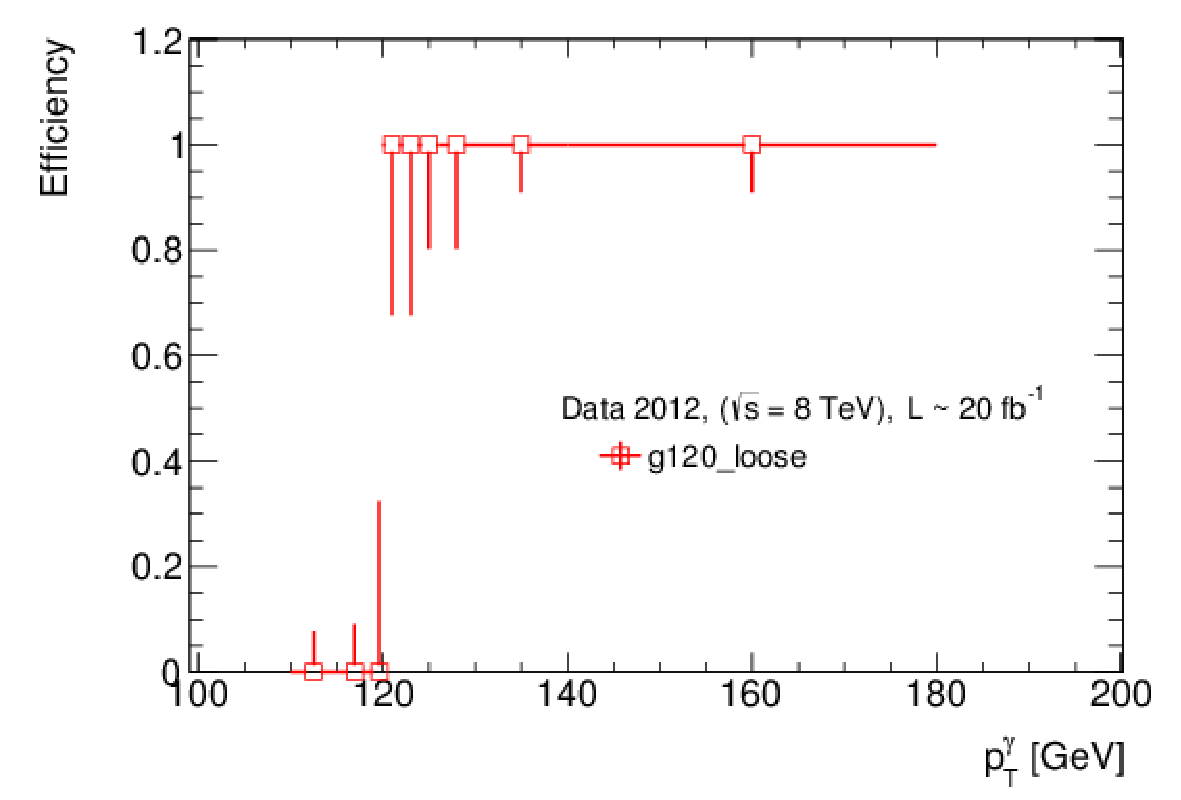
\includegraphics[width=0.6\textwidth]{EffPtg120_loose}

  \caption{Eficiencia del \emph{trigger} {\trigchain} como función del {\pt} del fotón.}
  \label{fig:trigger_perf}
\end{figure}


\section{Preselección}
\label{sec:base_seleccion}

\subsection{Vértice Primario}

Como se describe en la \cref{sec:obj_vertex} los candidatos a vértices de la interacción $pp$ son
reconstruidos en cada evento utilizando las trazas en el detector interno. El
vértice primario, correspondiente a la interacción dura de dispersión, es el
candidato con la mayor suma de $p_{T}^{2}$ para las trazas asociadas. Solo se
consideran los eventos donde el vértice primario tiene al menos cinco trazas
cargadas.


\subsection{Objetos}
\label{sec:preselection}
%% Antes de aplicar los cortes cinemáticos, se realiza la siguiente
%% preselección y limpieza.

En primero lugar se realiza una preselección de los objetos que se consideran en cada
evento como se detalla a continuación y se resume en la \cref{tab:base_sel}. Se
consideran fotones todos aquellos candidatos a fotón que pasen el criterio de
identificación \emph{tight}, que tengan $\pt>75\gev$ y $|\eta|<2.37$. Se
consideran electrones los candidatos que pasan el criterio de identificación \emph{medium}, y
que tengan un $\pt>10\gev$ y $|\eta|<2.47$, y muones a aquellos que pasan un criterio de
identificación \emph{loose} con $\pt>6 \gev$ y $|\eta|<2.5$. Para el caso de
jets, se consideran los que tienen $\pt>20\gev$ y $|\eta|<2.8$.


\begin{table}[!htbp]
  \centering

  \caption{Preselección de objetos. Criterio de identificación (ID) y cortes de
    aceptancia (\pt, $\eta$) considerados para cada tipo de partícula. Además
    del límite superior en $|\eta|$, no se consideran en ningún caso los objetos
    que se encuentren en la región entre la zona del \emph{barrel} y las \emph{end-caps} del detector, es
    decir, con $1.37 < |\eta| < 1.52$.}
  \label{tab:base_sel}

  \begin{tabularx}{0.8\textwidth}{LCCC}
    \hline
    & ID & $\pt$ & $|\eta|$ \\
    \hline
    Fotones    & \emph{tight}  & $> 75 \gev$ & $<2.37$ \\
    Electrones & \emph{medium} & $> 10 \gev$ & $<2.47$ \\
    Muones     & \emph{loose}  & $> 6  \gev$ & $<2.5$  \\
    Jets       & -             & $> 20 \gev$ & $<2.8$  \\
    \hline
  \end{tabularx}

\end{table}


%% La selección de los objetos se realiza según lo descripto en \cref{sec:obj_selection}.
%% El overlap removal y el event veto aplicado se detalla en la \cref{sec:overlap_romoval_event_veto}.

%% Excepto durante calculo de {\met}, dos cortes de aceptancia extra son requeridos
%% para los jets: $\pt > 40 \gev$ y $|\eta| < 2.8$.
%% Todos los jets pasando esta selección \emph{loose} son considerados cuando se aplica
%% la identificación de objetos descripta en \cref{sec:overlap_romoval_event_veto}.


\subsection{Eliminación de objetos superpuestos} %% y veto de eventos\note{?}}
\label{sec:overlap_romoval_event_veto}

De acuerdo a las definiciones de objetos presentadas más arriba, un objeto puede estar en
más de una categoría, contándose dos veces. Por este motivo se realiza un
procedimiento para remover este solapamiento, el cual se aplica sobre los
objetos preseleccionados antes de aplicar los criterios de aislamiento. El
procedimiento para remover estas ambigüedades entre los objetos es el que se
detalla a continuación en ese orden:

\begin{itemize}\itemsep0.1cm
\item Si un fotón o electrón se encuentran dentro de $\Delta R < 0.01$, el
  objeto es considerado como un electrón, removiéndose el fotón correspondiente.
  Esta elección reduce la taza de electrones mal reconstruidos como fotones.
\item Los jets que estén cerca ($\Delta R<0.2$) de un electrón o fotón
  preseleccionado se remueven.
\item Fotones y electrones preseleccionados son removidos si su distancia al jet
  más cercano es $0.2 < \Delta R < 0.4$.
\item Muones preseleccionados son removidos si su distancia al jet más cercano
  es $\Delta R < 0.4$.
\end{itemize}


%% \subsection{Limpieza de eventos}

Por último, para asegurar el correcto cálculo de la energía faltante, y reducir
los eventos con energía faltante instrumental, los eventos que satisfacen
alguna de las condiciones siguientes son descartados.

\begin{itemize}\itemsep0.1cm
\item Si el evento (después de de la preselección de objetos y la eliminación de los objetos superpuestos) contiene al menos
  un jet que falla los cortes de limpieza de jets que se definen en
  \cref{sec:jet_obj}.

\item Eventos con muones cósmicos: cuando el evento tiene al menos un muón con $|z_{0}| > \unit[1]{mm}$ o $|d_0| >
  \unit[0.2]{mm}$, donde estos valores son calculados con respecto al vértice
  primario. %%Estos muones tienen altas posibilidades de ser muones cosmicos \note{Check!}
\end{itemize}

Después de esta limpieza de eventos, con los objetos definidos en las secciones anteriores y después
de haber eliminado los objetos duplicados, se calcula la energía faltante transversa como se explica
en \cref{sec:met_obj}.



\section{Optimización de la selección de las regiones de señal}

Como primer paso se seleccionan eventos que contengan el estado final buscado:
un fotón, al menos un jet y energía faltante, y, a partir de esa selección
inicial, se eligen observables que permitan separar la señal del fondo y se
optimizan los cortes en estos observables.

Del estudio realizado en la \cref{sec:susy_studies}, resultan evidentes las diferencias
cinemáticas y topológicas de los eventos en las distintas regiones del
espacio de parámetros {\mgmn} del modelo de SUSY.
Es por esta razón que resulta conveniente tener más de una región de señal,
cada una destinada a una zona particular del espacio de parámetros.

Por tal motivo, se dividió el análisis en dos regiones de señal, a las que se
llamó {\SRL} y {\SRH}. La primera de ellas, \SRL, se focaliza en la zona en la que
los gluinos decaen en cascada hasta neutralinos NLSP de baja y
moderada masa. Los eventos de señal en esta región se caracterizan por una gran
multiplicidad de jets y actividad hadrónica, debido a que involucra cadenas de
decaimiento largas de gluinos pesados a través de la producción de charginos y quarks.
Cuanto más baja la masa del {\ninoone}, más baja sera la energía del fotón y
menor es la cantidad de energía faltante. La segunda región de señal, \SRH,
tiene como motivación aquellos escenarios donde la masa del gluino y del neutralino
más liviano están cerca una de la otra. La cadena de decaimiento es por lo tanto
mucho más corta en este caso, con una menor multiplicidad de jets y, debido al
neutralino pesado, fotones de alto {\pt} y gran cantidad de energía faltante en
el estado final.

En la \cref{fig:srs_motivation} puede verse esquemáticamente a que región del espacio
de parámetros de la señal {\mgmn} está destinada cada SR.

\begin{figure}[!htbp]
  \centering
    \resizebox{0.5\textwidth}{!}{
      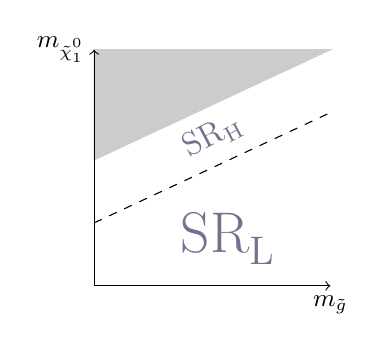
\begin{tikzpicture}

  \colorlet{green}{green!50!black!50}
  \colorlet{red}{red!70!black!50}
  \colorlet{blue}{blue!70!black!80}

  \draw[gray!40,fill] (0, 1.6) -- (3, 3) -- (0,3) -- cycle;

  \draw[->] (0,0) -- (3,0) node[below] {\small $m_{\tilde{g}}$};
  \draw[->] (0,0) -- (0,3) node[left] {\small $m_{\tilde{\chi}_1^0}$};

  %\draw[red,line width=2] (1.5,1.8) circle (15pt);
  \draw[dashed] (0,0.8) -- (3, 2.2);

  \node[blue] at (1.7,0.6) {\huge SR$_{\mathrm{L}}$};
  \node[blue] at (1.5,1.9) [rotate=28] {\large SR$_{\mathrm{H}}$};

\end{tikzpicture}

      }
    \caption{Esquema de la región del espacio de parámetros del modelo de señal en el
    plano {\mgmn} y a que zona esta dirigido el diseño de las dos regiones de señal.}
  \label{fig:srs_motivation}
\end{figure}


Para la optimización de las SR, se utilizaron varios puntos de señal en cada región,
representativos de la topología y el espacio de fase en cada caso:

\begin{itemize}\itemsep0.2cm\parskip0.2cm
\item {\SRL}: $(1150, 200)$ y $(1150, 450)$
\item {\SRH}: $(1150, 850)$ y $(1150, 1050)$
\end{itemize}
%
donde cada punto queda determinado por sus valores $(M_3, \mu)$.

Como fondo se utilizaron las muestras MC, y se consideró una incerteza en la estimación del
fondo de 25\%. Todas las muestras MC fueron normalizadas a una luminosidad total
integrada de 20.3 \ifb. La significancia esperada se calculó utilizando la
\cref{eq:Za}, y para evitar una selección muy restringida, se requiere al menos
un evento de fondo en cada SR. Además de evaluar la significancia esperada para
distintos cortes también se tuvo en cuenta que la eficiencia de señal sea
superior al 20\%.

Los cortes fueron optimizados en el orden de poder discriminatorio, uno a la
vez, y aplicados en el orden descripto a continuación, monitoreando la
significancia para distintos cortes en las variables discriminatorias.

Como ya se ha mencionado, el estado final buscado en este análisis consiste en un
único fotón, jets y energía faltante. Por lo que la definición de las SR
comienza optimizando los cortes en las variables cinemáticas del fotón, los jets
y el corte en energía faltante.

%% Como primer paso se impuso un corte en la energia faltante transversa $\met>150\gev$Se impuso
%% La significancia para cada caso
%% The significance for different cut combinations was also monitored to take the best configuration.
%% A minimal pre-selection cut in $\met>150\gev$ was placed in the SR, which is highly efficient for the signal and very effective
%% removing large part of the SM backgrounds, particularly the QCD multijet production. The final selection requirements are summarised in sec \ref{sec:signal_regions}.

%% \begin{figure}[h!]
%%   \centering
%%   \includegraphics[width=0.5\textwidth]{figures/grid_regions.pdf}
%%   \caption{Regiones de senal usadas en este analisis.
%%     Los cuadrados azules corresponden a cada muestra de senal simulada en la
%%     grid \M{3}-$\mu$.
%%     El área gris es una región cismáticamente prohibida ($m_{\gluino}<m_{\ninoone}$).}\label{fig:SRegions}
%% \end{figure}


\subsection{Fotón}\label{sec:opt_ph_iso}

El primer paso para definir la SR consistió en seleccionar eventos con un único
fotón de los previamente seleccionados con {\pt} mayor a 125 \gev. Este valor
fue elegido para asegurar la máxima eficiencia del trigger.
%% En la \cref{fig:photon_pt} se muestra las distribuciones del {\pt} del fotón
%% para los eventos de fondo del {\SM} como también para algunos puntos de señal.

Los eventos con un segundo fotón con $\pt > 75 \gev$ fueron vetados. El corte en
{\pt} de $75\gev$ fue elegido para que las SR sean ortogonales a las SR del
análisis de ATLAS que busca dos fotones\cite{ATLAS-CONF-2014-001} garantizando la
posible combinación estadística entre ambos. Este análisis fue diseñado para
buscar SUSY en escenarios GGM, pero particularmente en el caso de que el
neutralino NLSP sea mayoritariamente bino, y el decaimiento a fotones sea
dominante.


%% \begin{figure}[!htbp]
%%   \centering
%%   \includegraphics[width=0.45\textwidth]{figures/ph_pt_base1}
%%   \includegraphics[width=0.45\textwidth]{figures/ph_pt_base2}
%%   \caption{Distribución del {\pt} del fotón para señal y fondo MC en {\SRL} (izquierda) y
%%     {\SRH} (derecha), correspondiente a una luminosidad integrada de {\ilumi} antes de que ningún
%%     corte haya sido aplicado. }
%%   \label{fig:photon_pt}
%% \end{figure}

Como se menciona en la \cref{sec:fotones}, para seleccionar los fotones se
aplica un corte en la energía transversa de aislamiento (\etiso). Especificamente,
para el presente análisis se estudiaron distintos
criterios de aislamiento, variando el tamaño del cono ($R$) en el cual se
calcula esta energía.

%% La optimización de este criterio de aislamiento  fue realizada mirando el desempe\~no
%% de los distintos tamaños de cono.

En la \cref{fig:photon_iso} se muestran las distribuciones de la energía de
aislamiento para varios valores de $R$ para las muestras de señal en las dos SR.
La SR con mayor diferencia de masa entre gluino y neutralino parece tener
distribuciones más anchas, un efecto que desaparece para tamaños de cono mas
chicos. Como se ve en la \cref{fig:photon_iso_sig} (arriba), la mayor eficiencia
de selección se obtiene también para el menor tamaño de cono, $R = 0.2$. Para un
corte de $5 \GeV$, se obtiene una eficiencia alta (85-90\%) a lo largo de toda la
grid. Luego de aplicar una preselección en {\met}, los fotones no aislados
provenientes de fondos dominados por procesos QCD son muy suprimidos, reduciendo el impacto
del corte de aislamiento en la significancia.

Incluso luego de que la corrección es aplicada para remover la filtración de
energía del fotón dentro de su propio cono de aislamiento, una dependencia remante
con el {\pt} del fotón es observada para todos los tamaños de cono
considerados, como se muestra en \cref{fig:photon_iso} (abajo). El tratamiento
de este efecto es discutido en la \cref{sec:jfake_sig_template,sec:expsyst}.


\begin{figure}[!htbp]

  \centering
  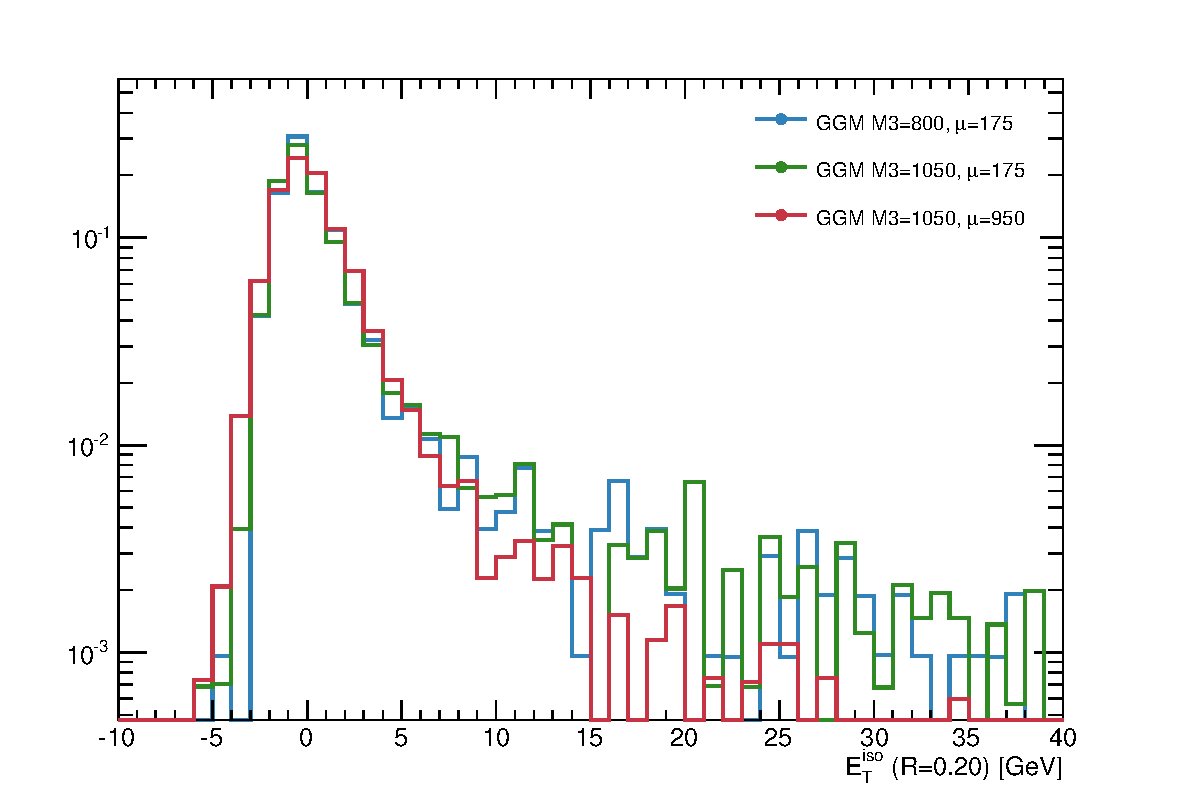
\includegraphics[width=0.32\textwidth]{figures/iso_20}
  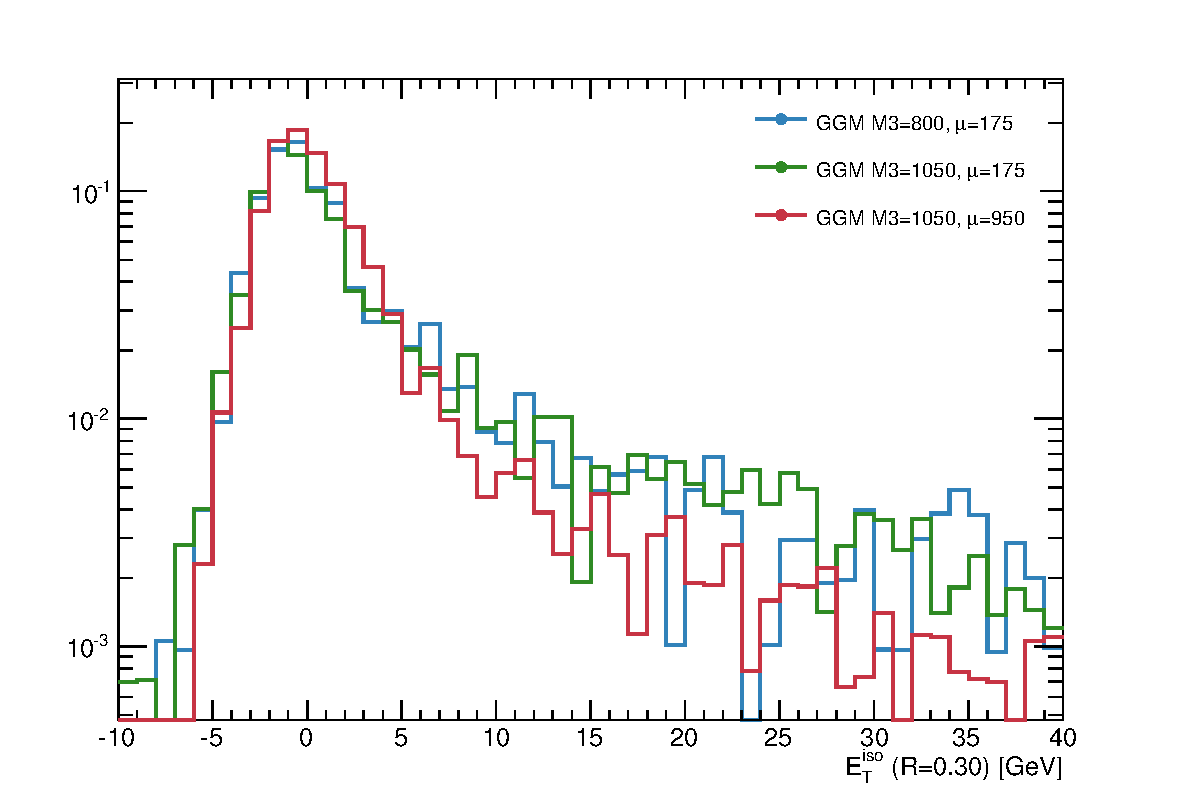
\includegraphics[width=0.32\textwidth]{figures/iso_30}
  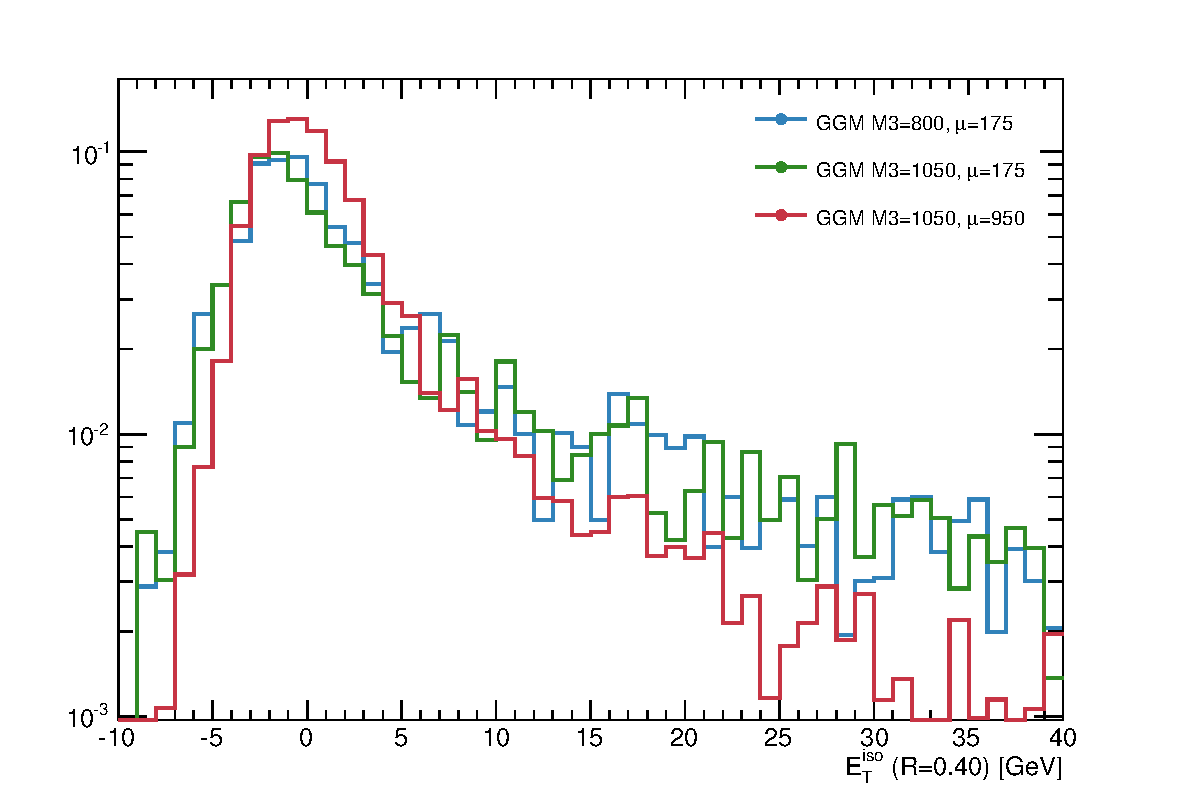
\includegraphics[width=0.32\textwidth]{figures/iso_40}

  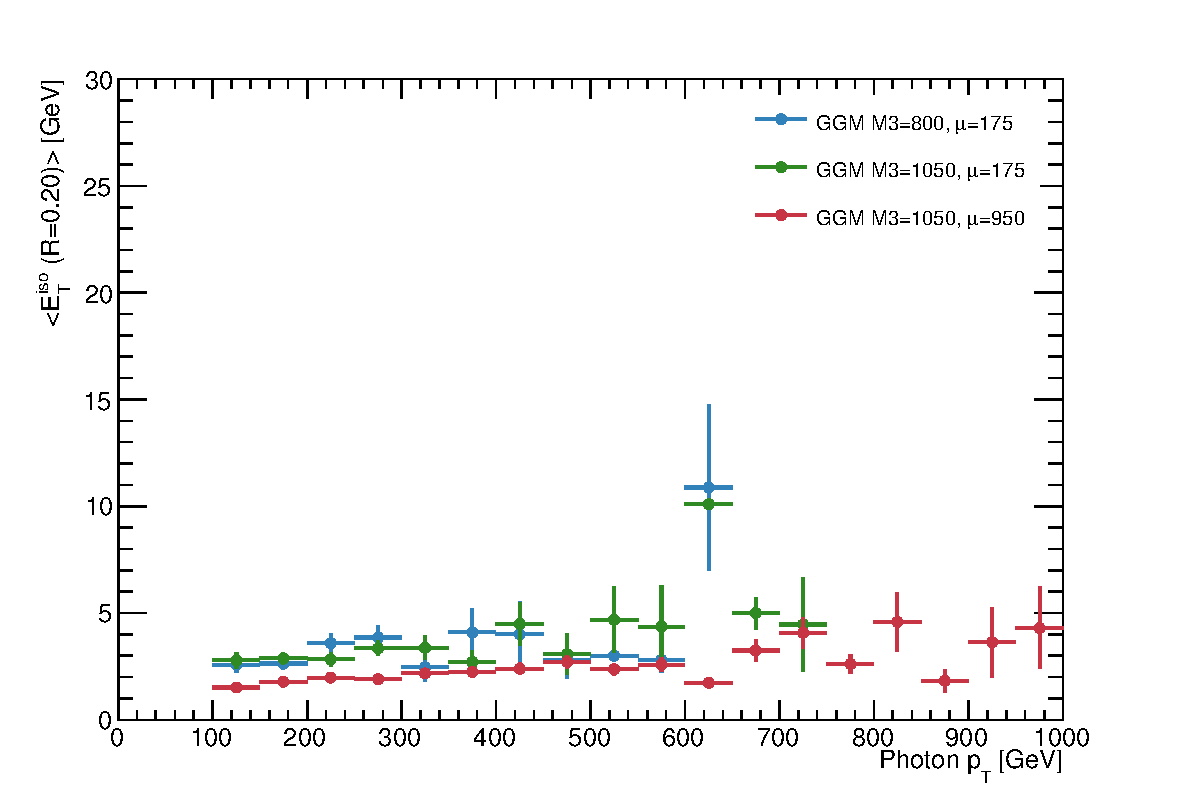
\includegraphics[width=0.32\textwidth]{figures/iso_20_pt}
  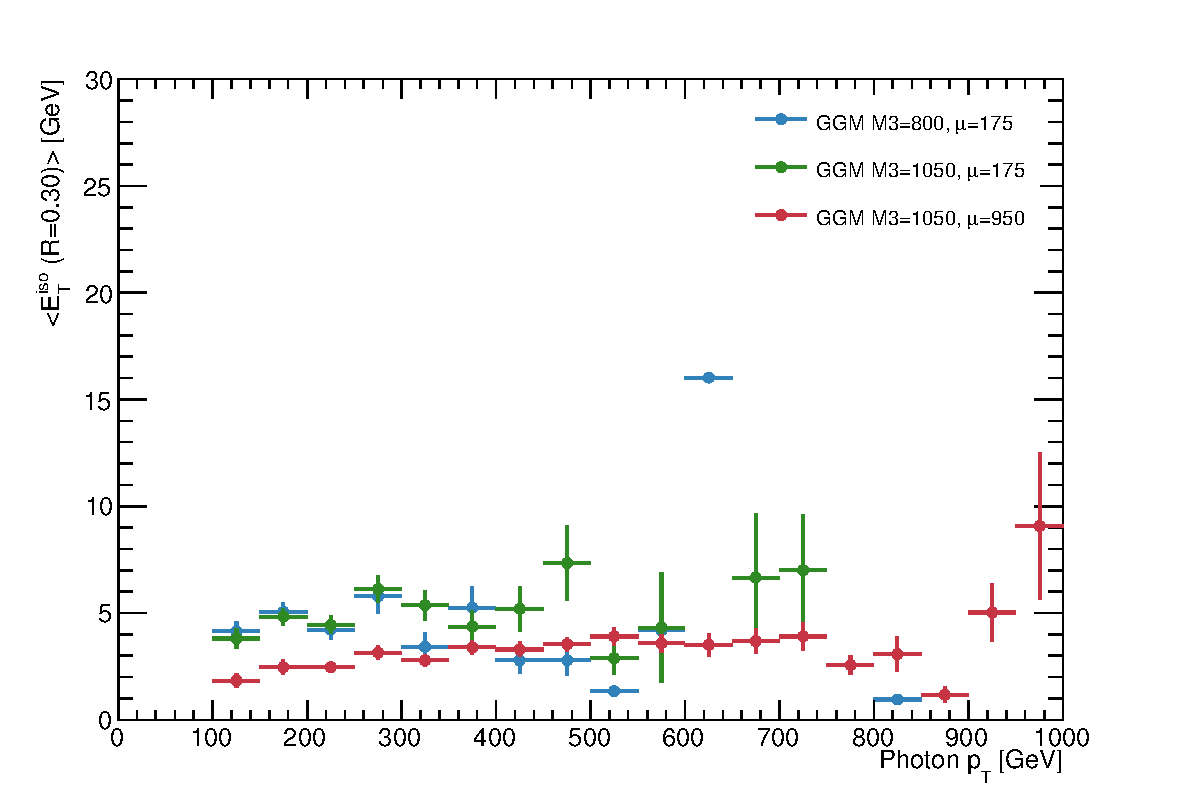
\includegraphics[width=0.32\textwidth]{figures/iso_30_pt}
  \includegraphics[width=0.32\textwidth]{figures/iso_40_pt}

  \caption{Distribución de {\etiso} (arriba) y su valor medio como función del
    {\pt} del fotón (abajo) para distintos tamaños de conos: $R=0.2$, $R=0.3$ y$R=0.4$.
    Una preselección de $\pt>125\gev$ y $\met>150\gev$ fue aplicada, para suprimir
    gran parte del fondo de fotones directos.}
  \label{fig:photon_iso}
\end{figure}

\begin{figure}[!h]
  \centering

  \includegraphics[width=0.3\textwidth]{figures/iso_20_sig}
  \includegraphics[width=0.3\textwidth]{figures/iso_30_sig}
  \includegraphics[width=0.3\textwidth]{figures/iso_40_sig}

  \includegraphics[width=0.3\textwidth]{figures/iso_20_eff}
  \includegraphics[width=0.3\textwidth]{figures/iso_30_eff}
  \includegraphics[width=0.3\textwidth]{figures/iso_40_eff}

  \caption{Significancia esperada (arriba) y eficiencia (abajo) como función del
    corte en la energía de aislamiento, después del corte en {\pt} y {\met}.}
  \label{fig:photon_iso_sig}
\end{figure}



\subsection{Leptones}\label{sec:leptonphoton_veto}

Además del veto a los eventos con un segundo fotón, también se remueven
los eventos que contienen leptones ($e$ o $\mu$) con el objetivo de que las
SR no tengan un solapamiento con las SR del análisis que busca estados finales
con un fotón, un leptón y energía faltante \cite{ATLAS-CONF-2012-144}.



\subsection{Energía faltante}

La principal característica de los eventos de SUSY donde se conserva
la paridad-R es la presencia de una gran cantidad de energía faltante debido
a las LSP estables que escapan la detección, en este caso debido a los dos gravitinos
en el estado final.
Un corte en esta variable reduce enormemente la contaminación de procesos
QCD y también de otros procesos del {\SM}.
La \cref{fig:opt_met} muestra la distribución de {\met} en eventos con
un fotón aislado con alto {\pt} (como se definió en la sección anterior),
para dos puntos de señal en cada SR, junto al fondo esperado de simulaciones
MC.

Un corte en {\met} relativamente bajo ($> 200 \gev$) es capaz de separar
la señal y el fondo significativamente en {\SRL}, mientras que para {\SRH}
es posible aplicar un corte más alto ($>300\gev$).

\begin{figure}[!h]
  \centering
  \includegraphics[width=0.49\textwidth]{met_et_base1}
  \includegraphics[width=0.49\textwidth]{met_et_base2}
  \caption{Energía faltante transversa
    luego de aplicar el corte en el {\pt} del fotón y en la energía de aislamiento
    para el fondo y los puntos de señal de {\SRL} (izquierda) y {\SRH} (derecha),
    para una luminosidad integrada de {\ilumi}.}

  \label{fig:opt_met}
\end{figure}



\subsection{Multiplicidad y {\pt} de los jets} \label{sec:opt_njet}

En la \cref{fig:jets_npv} se muestra el valor medio del número de jets
seleccionados como función del número de vértices en el evento, para distintos
cortes en el {\pt} de los jets. Notar que el número de vértices en un evento
está relacionado con el \emph{pile-up}. A medida que aumenta el corte en {\pt}
el número de jets se hace más estable con el \emph{pile-up}, y por lo tanto en
este análisis se consideran los jets con $\pt>40\gev$

%% El corte en {\pt} fue elegido para asegurar una selección robusta contra el pile-up.


\begin{figure}[!h]
  \centering
  \includegraphics[width=0.5\textwidth]{data_jets_npv}
  \caption{Valor medio del número de jets vs. el número de vértices primarios
    observados en datos para distintas selecciones de $\pt^{\mathrm{jet}}$.}
    \label{fig:jets_npv}
\end{figure}



%% Como se muestra en la \cref{fig:jets_npv}, el número medio de jets seleccionados
%% es de esta forma una distribución \hl{flat} como función del número de vértices
%% primarios. Luego, en la selección final, cortes más alto en el {\pt} de los jets
%% son utilizados como se describe en \cref{sec:opt_njet}.

La \cref{fig:opt_jet_n} muestra la multiplicidad de jets (\njets)
para $\pt^{\mathrm{jet}} > 40$ \gev, después de los cortes optimizados en el
fotón y la {\met} descriptos anteriormente. Mientras que la señal tiene
típicamente un gran número de jets, la mayoría de los fondos W/Z+jets, diboson y
QCD se acumulan en la zona de pocos jets. Al menos dos (cuatro) jets son
requeridos para los eventos que pasan la selección de {\SRL} ({\SRH}). Una mayor
multiplicidad es efectivamente esperada para {\SRL} debido a que su objetivo es
la región de gluinos pesados donde el decaimiento dominante es el de producción
de charginos por un decaimiento de tres cuerpos.

\begin{figure}[!h]
  \centering
  \includegraphics[width=0.49\textwidth]{jet_n_base1}
  \includegraphics[width=0.49\textwidth]{jet_n_base2}
  \caption{Distribuciones del número de jets con $\pt > 40 \gev$ en {\SRL} (izquierda) y {\SRH} (derecha),
    después de la seleccion en el {\pt} del fotón y $\met > 150\gev$,
    para una luminosidad integrada de {\ilumi}.}
  \label{fig:opt_jet_n}
\end{figure}

%{\fig} \ref{fig:jetlead_3SR}  shows the \pt\ of the leading jet, after the photon \pt\ and \etmiss cut,
%and requiring the number of jets to be equal or larger than two for SR1-SR3, and equal or larger than
%four for SR2. Additional signal-background discrimination can be obtained by imposing cuts on the %leading
%jet \pt\ (\pt$(j1)$)since the signal tends to have hard leading jets, in particular for the case involving large
%gluino masses and low to medium neutralino masses (SR2).  For SR1 and SR2 the leading jet \pt\  is %required
%to be larger than 80 \gev~ and 100 \gev, respectively.   After those cuts, in  {\fig} \ref{fig:jetsublead_3SR},
%the subleading jet \pt\  (\pt$(j2)$) distributions for the three signal regions are shown. A further cut is %applied for
%SR1 and SR2, by requiring $\pt(j2)>80$ \gev~  and $> 100$ \gev, respectively.

%% La \cref{fig:opt_jet_p1} muestra el {\pt} del jet más energético ($\pt^{j1}$),
%% después de los cortes descriptos anteriormente. %Adicionalmenteafter the
%% photon \pt, \etmiss\ and $N_{jet}$ requirements described above for each signal region.

En la {\SRL} es posible obtener una discriminacion requiriendo además que los dos jets
más energéticos tengan $\pt>100 \gev$.

%% En la {\SRH} donde la masa del gluino y la NLSP
%% es menor, een
%% Additional signal-background discrimination can be achieved by requiring a hard leading
%% jet, particularly for SR2 where the heavy gluinos decay down to relatively light neutralinos.
%% Thus, the leading jet \pt\ in SR2 is required to be larger than 100 \gev. Although a
%% harder requirement is suggested by {\fig} \ref{fig:jetlead_3SR}, it was found better to
%% keep it relatively loose and rely on the shape variables described in sec \ref{sec:shape_vars}.
%% The smaller mass difference between gluino and the lightest neutralino in SR3 leads to a
%% softer jet spectrum and then no further requirement is applied in this region.
%Additional signal-background discrimination can be obtained by imposing cuts on the leading  jet \pt\ since the signal tends to have hard leading jets, in particular for the case involving  large gluino masses and low to medium neutralino masses (SR2).  For SR1 and SR2 the leading jet \pt\  is required to be larger than 80 \gev~ and 100 \gev, respectively.

%% \begin{figure}[!htbp]
%%   \centering
%%   \includegraphics[width=0.49\textwidth]{figures/figura} %jet1_pt_SR2}
%%   \includegraphics[width=0.49\textwidth]{figures/figura} %jet1_pt_SR3}
%%   \caption{Momento transverso del jet más energético en {\SRL} (izquierda) y {\SRH} (derecha),
%%     para una luminosidad integrada de {\ilumi}.}
%%   \label{fig:opt_jet_pt1}
%% \end{figure}

%% A continuacion se exploro el momento transverso del segundo jet más energetico ($\pt^{j2}$).
%% Las distirbuciones para cada region pueden verse en \cref{fig:opt_jet_pt2}. En {\SRL}
%% se encontro que un corte en $\pt^{j2}>100$ \gev

%% \begin{figure}[!htbp]
%%  \centering
%%  \includegraphics[width=0.49\textwidth]{figures/figura} %jet2_pt_SR2}
%%  \includegraphics[width=0.49\textwidth]{figures/figura} %jet2_pt_SR3}
%%   \caption{Momento transverso del segundo jet más energético en {\SRL} (izquierda) y {\SRH} (derecha),
%%     para una luminosidad integrada de {\ilumi}.}
%%  \label{fig:opt_jet_pt2}
%% \end{figure}



\subsection{Separación angular entre jets y \met}
\label{sec:dphi_obj}

Como ya ha sido mencionado, en los eventos de señal, la energía faltante es producida por los dos
gravitinos que escapan la detección. Se espera por lo tanto que la dirección de {\met} sea aleatoria,
sin estar correlacionada con ninguno de los demás objetos del evento. Por otro
lado, si la {\met} es originada a partir de efectos instrumentales o de neutrinos
energéticos en $b$-jets o $c$-jets, la dirección de {\met} estará
correlacionada con uno de los jets mal reconstruidos. La
\cref{fig:opt_dphi_jetmet} muestra el mínimo $\Delta\phi$ entre la dirección
de {\met} y la de los dos jets más energéticos.

%% \begin{equation} \label{eq:dphi}
%%   %%\min\left[ \cos   \Delta\phi({\rm jet}_{1,2},\MET) \right] \equiv  \min \left[\frac{\vec{\met} \cdot \vec{p}_{\rm T}^{\rm \; jet,i}}{|\vec{\met}|  |\pt^{\mathrm{jet},i}|}\right] \quad \quad i = 1,2
%%   \cos \Delta\phi(\mathrm{jet},\met) \equiv \frac{\vec{\met} \cdot \vec{p}_\mathrm{T}^{\mathrm{jet}}}{|\vec{\met}| |\pt^{\mathrm{jet}}|}
%% \end{equation}
%% %

%% after applying the photon \pt, \met, jet {\pt} and multiplicity cuts.
%% A lower bound $\dphijm>0.4$ cut is applied for the two signal regions,
%% which helps to significantly reduce the QCD background and clean events with mis-reconstructed \etmiss.

\begin{figure}[!h]
  \centering

  \includegraphics[width=0.49\textwidth]{figures/dphi_jetmet_srl}
  \includegraphics[width=0.49\textwidth]{figures/dphi_jetmet_srh}

  \caption{Separación angular $\Delta \phi \mathrm{(jet, \met)}$ para el fondo y los puntos de se\~nal para {\SRL} (izquierda) y {\SRH} (derecha),
    para una luminosidad integrada de {\ilumi}.}
  \label{fig:opt_dphi_jetmet}
\end{figure}


\subsection{Separación angular entre jets y fotón}

Para regiones del espacio de parámetros del modelo de señal
donde los gluinos y los neutralinos tienen alta masa ({\SRH})
un corte en la separación entre el fotón y los jets ayuda a
reducir el fondo, principalmente aquel proveniente de dijets y
fotones directos, donde un fotón (real o falso) tiende a ser
producido en la dirección opuesta al jet más energético.
La distribución para la {\SRH} se puede ver en \cref{fig:opt_dphi_gamjet}.

%% \begin{equation} \label{eq:dphi}
%%   \cos \dphijg \equiv \frac{\vec{p}_\mathrm{T}^{\gamma} \cdot \vec{p}_\mathrm{T}^\mathrm{jet}}{|{p}_\mathrm{T}^{\gamma}| |\pt^\mathrm{jet}|}
%% \end{equation}

%

%% for {\SRH} benchmark signal samples after all previous selection.
%% The cut value chosen for this high gluino-neutralino mass region is $\dphijg<2$.

 % shows the jet-photon $\phi$ separation for signal and backround in SR3, after applying the photon \pt\ ,  \etmiss,  jet  \pt\  and multiplicity as well as  $\Delta \phi \text{(jet, MET)}$ cuts.  The cut value chosen for jet-photon separation in this high mass signal region  is  $\Delta \phi \text{(jet}, \gamma) >2$.

\begin{figure}[!h]
  \centering

  \includegraphics[width=0.49\textwidth]{figures/dphi_gamjet_srh}

  \caption{Distribución de {\dphijg} para {\SRH}, despues de aplicar la selección completa, excepto este corte,
    para una luminosidad integrada de 20.3 \ifb.}
  \label{fig:opt_dphi_gamjet}
\end{figure}



\subsection{Energía total transversa (\HT)}
\label{sec:ht_obj}

Dada la gran masa de los gluinos producidos en las colisiones, en el espacio de
parámetros explorado en este análisis, se espera que la energía transversa
visible total sea alta. Por eso, el observable {\HT} definido como la suma
escalar del momento transverso de todos los objetos observados en el estado
final es mucho mayor para eventos de señal que para los eventos de fondo.
Después del veto a los eventos con leptones, {\HT} se define como:

\begin{equation}
  \HT \equiv |\pt^{\gamma}| + \sum_{\mathrm{jets}} |\pt^\mathrm{jet}|
  \label{eq:ht_def}
\end{equation}

La \cref{fig:opt_ht} muestra las distribuciones de {\HT} para las dos regiones de señal.
Para {\SRL}, se espera incluso que {\HT} sea mayor, debido a la
diferencia de masa entre el gluino y el neutralino NLSP. Sin embargo
se encontró una variable más efectiva para la separación entre señal y
fondo que se describe a continuación y por lo tanto no se aplica un corte
en esta variable.

%photon \pt,  \etmiss, jet multiplicity, two leading jets  \pt,   jet-\etmiss\  and jet-photon $\phi$ separation cuts.

En {\SRH} un corte en este observable $\HT>800\gev$ ayuda a reducir el fondo restante.
Dada la masa alta del neutralino, la mayor contribución de {\HT} proviene
del fotón muy energético producido en el evento.


\begin{figure}[!h]
  \centering

  \includegraphics[width=0.49\textwidth]{ht_srl}
  \includegraphics[width=0.49\textwidth]{ht_srh}

  \caption{Distribución de la energía total transversa (\HT) para {\SRL} (izquierda)
    y {\SRH} (derecha) para una luminosidad total integrada de 20.3 \ifb. Todos los cortes de la selección
  de la SR son aplicados exceptuando el corte en {\HT}.}
  \label{fig:opt_ht}
\end{figure}



\subsection{Variables de forma adicionales}\label{sec:shape_vars}

Varias variables de forma fueron exploradas para poder obtener
una discriminación adicional entre señal y fondo. En especial se estudió el
observable $R_T^n$ definido como

\begin{equation}\label{eq:rt_formula}
  R_\mathrm{T}^{n} = \frac{\sum_{i=1}^{n}p_\mathrm{T}^{\text{jet}_i}}{\sum p_\mathrm{T}^{\text{jet}}},
\end{equation}
%
es decir, el cociente entre la suma escalar de los {\pt} de $n$ jets y la suma
escalar del {\pt} de todos los jets en el evento, donde $n$ es el mínimo número
de jets requerido.

Es evidente que la distribución de esta variable (como se explica en
\cite{PhysRevD.84.055010}), depende de la multiplicidad y el momento transverso
de los jets. En el caso que $n \sim \njets$ el denominador y el
numerador son casi idénticos y el cociente es $\sim 1$, y es exactamente 1
cuando son iguales.
Para los procesos de señal en los que $n$ es mucho menor al número de jets en el
evento, la distribución será menor a 1.

%% depends on the multiplicity and hardness of the jets. As shown in previous
%% sections, the SUSY signals here considered are characterized by hard multijet
%% events in a wide region of parameter space. Evenmore, the sub-leading jets are
%% comparatively harder than those in SM background events.


\begin{figure}[!h]
  \centering

  \includegraphics[width=0.49\textwidth]{figures/rt4_srl}
  \includegraphics[width=0.49\textwidth]{figures/rt2_srh}

  \caption{Distribución de {\rt} para {\SRL}  (izquierda) y {\rtt} para {\SRH} (derecha)
    para una luminosidad total integrada de 20.3 \ifb. Todos los cortes de la selección
    de la SR son aplicados exceptuando el corte en $R_\mathrm{T}$.}
  \label{fig:opt_rt}
\end{figure}

La \cref{fig:opt_rt} (izquierda) muestra la distribución de {\rtt} para {\SRH},
después de la selección final excepto el corte en {\rtt}. Mientras que la
\cref{fig:opt_rt} muestra la distribución de {\rt} para {\SRL}. El bajo número
de jets para {\SRH}, hace que la distribución de {\rtt} para los eventos de
señal sea similar a la del fondo QCD, y por lo tanto el observable no es útil
para rechazar fondo manteniendo una aceptancia razonable. Para el caso de {\SRL}
un corte $\rt < 0.85$ permite reducir en una fracción considerable el fondo con
una pérdida muy chica en la eficiencia de señal.



\section{Selección final de las regiones de se\~nal}\label{sec:signal_regions}

Como resultado del proceso de optimización descripto en la sección anterior,
se definen las dos regiones de señal:

\begin{description}\itemsep0.2cm

\item[{\bf {\SRL}}] motivada por los eventos en los que gluinos
  decaen a neutralinos de baja/media masa. Estos eventos están
  caracterizados por una gran multiplicidad de jets energéticos, mientras que la energía
  del fotón y la energía faltante dependerá de la masa del neutralino, pero en general
  será relativamente baja.


\item[{\bf {\SRH}}] motivada por eventos en los que los gluinos
  producidos decaen en neutralinos con una masa similar a estos. Dichos eventos están caracterizados
  por un fotón de alto {\pt} y gran cantidad de {\met}, con una menor multiplicidad de jets.
\end{description}

Cada región de señal queda definida entonces por los cortes de selección detallados en la \cref{tab:final_sel_sr}.

\begin{table}[!htbp]

  \centering
  \caption{Conjunto de cortes en los observables que definen las dos regiones de señal, {\SRL} y {\SRH}.}
  \label{tab:final_sel_sr}

  \begin{tabularx}{0.6\textwidth}{LCC}
    \hline
    & {\SRL} & {\SRH} \\
    \hline
    {\nphotons} & $=1$ & $=1$ \\
    \ptgam & $>125 \gev$ & $>300 \gev$ \\
    {\nleptons} & $=0$ & $=0$ \\
    {\njets} & $\geq 4$ & $\geq 2$ \\
    $\pt^{\mathrm{jet}_1}$ & $>100 \gev$ & - \\
    $\pt^{\mathrm{jet}_2}$ & $>100 \gev$ & - \\
    $\Delta\phi(\mathrm{jet}, \met)$ & $>0.4$ & $>0.4$ \\
    {\met} & $>200 \gev$ & $> 300 \gev$ \\
    $R_\mathrm{T}^4$ & 0.85 & - \\
    $\HT$ & - & $>800 \gev$ \\
    $\Delta\phi(\gam,\mathrm{jet})$ & - & $<2.0$ \\
    \hline
    \end{tabularx}

\end{table}


El número esperado de eventos de fondos del {\SM} estimado a partir de de las
muestras simuladas después de la selección final se muestra en la
\cref{tab:exp_bkg_sr}, para {\SRL} y {\SRH},
respectivamente. También se presenta el número de eventos esperado de señal y la
significancia esperada para los dos puntos de referencia en cada SR.
Adicionalmente, en la \cref{tab:mc_events_sr_phtype} se puede ver el número de
eventos de fondo esperado separando fotones reales de los eventos donde un jet o
un electrón es identificado erróneamente como un fotón.
%% El primer tipo de eventos es claramente
%% dominante en este análisis, en presencia de energía faltante tanto real como
%% instrumental.
Se puede ver que la contaminación dominante proviene de {\vgam} ($V=W \text{ o }
Z$) y {\ttgam}. La contaminación de {\vgam} en {\SRL} es de 0.13, de los cuales
0.10 corresponden a {\wgam} y 0.03 a {\znngam}. Para {\SRH} el número de eventos
de {\vgam} es de 0.66, de los cuales 0.44 de {\wgam} y 0.22 de {\znngam}. En la
{\SRL} también existe una contaminación de eventos de procesos {\ttbar} en los
que un electrón es identificado como fotón.

La significancia esperada de descubrimiento para los distintos puntos
de la \emph{grid} de señal en el plano {\mgmn} se puede ver en la
\cref{fig:opt_discovery_exp}, junto con los contornos en los que la significancia
es de $3\sigma$ y $5\sigma$.

Es
importante notar que estos resultados son preliminares y obtenidos de
simulaciones Monte Carlo. Los resultados finales son derivados utilizando los
métodos de estimación de fondos descriptos en el \cref{cap:fondos}, y luego
del ajuste combinado, y son descriptos en el \cref{cap:resultados}.

\begin{table}[!h]
  \centering
  \caption{Número de eventos esperado para los fondos del {\SM}
    y algunos puntos de señal después de cada corte de la región
    de señal {\SRL} (arriba) y {\SRH} (abajo), para una luminosidad integrada de {\ilumi}. Para los
    puntos de señal, también se muestra en la última fila, la
    significancia esperada.}

  \label{tab:exp_bkg_sr}

  \resizebox{\textwidth}{!}{
    \begin{tabular}{lrrrrrrrrr}
      \hline
      \multicolumn{1}{c}{\textbf{\SRL}}   & \multicolumn{1}{c}{(1150, 200)} & \multicolumn{1}{c}{(1150,450)} &  \multicolumn{1}{c}{V\gam} & \multicolumn{1}{c}{Diboson} & \multicolumn{1}{c}{V + jets} & \multicolumn{1}{c}{\gjet, multijet} & \multicolumn{1}{c}{\ttbar} & \multicolumn{1}{c}{\ttgam} & \multicolumn{1}{c}{Fondo total} \\
      \hline
      $=1$ fotón        &  22.87 & 33.75 & 8396.04 & 230.19 & 10093.10 & 3103339.25 & 251.46 & 847.09 & $3123157.13\pm2013.86$ \\
      0 leptones        &  13.66 & 20.88 & 5433.21 & 166.08 &  7808.01 & 3101910.25 & 204.99 & 442.29 &  $3115964.83\pm1971.53$ \\
      \met              &   7.74 & 14.96 &  457.80 &  11.07 &   188.39 &      94.27 &   6.50 &  22.21 &        $780.24\pm55.42$ \\
      $N_\mathrm{jets}$ &   7.72 & 14.88 &   13.83 &   1.17 &     0.00 &       8.17 &   2.52 &   8.08 &         $33.76\pm12.09$ \\
      $\pt^{\mathrm{jet}_1}$       &   7.72 & 14.86 &   12.97 &   1.17 &     0.00 &       8.17 &   2.44 &   7.44 &         $32.19\pm11.83$ \\
      $\pt^{\mathrm{jet}_2}$       &   7.68 & 14.71 &    9.00 &   1.14 &     0.00 &       7.94 &   1.97 &   5.63 &         $25.69\pm10.66$ \\
      $\dphijm$         &   6.73 & 12.98 &    7.00 &   0.93 &     0.00 &       2.77 &   1.83 &   3.84 &         $16.37\pm8.58$ \\
      $R_T^4$           &   5.27 & 10.09 &    0.13 &   0.00 &     0.00 &       0.00 &   0.16 &   0.46 &          $0.75\pm1.46$ \\
      \hline
      Significancia                 &   3.81 &  6.14 &  &  &  &  &  &  &  \\
      \hline

    \end{tabular}
  }
  %%
  \vspace{0.4cm}
  %%
  \resizebox{\textwidth}{!}{
    \begin{tabular}{lrrrrrrrrr}

      \hline
      \multicolumn{1}{c}{\textbf{\SRH}}  & \multicolumn{1}{c}{(1150, 850)} & \multicolumn{1}{c}{(1150,1050)} &  \multicolumn{1}{c}{V\gam} & \multicolumn{1}{c}{Diboson} & \multicolumn{1}{c}{V + jets} & \multicolumn{1}{c}{\gjet,multijet} & \multicolumn{1}{c}{\ttbar} & \multicolumn{1}{c}{\ttgam} & \multicolumn{1}{c}{Fondo total} \\
      \hline
        $=1$ fotón         & 26.87 & 11.68 & 352.27 & 6.86 & 153.18 & 79255.07 & 0.73 & 49.23 & $79817.34\pm323.16$ \\
        0 leptones         & 22.92 & 11.20 & 215.86 & 4.40 & 102.50 & 79161.53 & 0.53 & 23.77 & $79508.59\pm313.87$ \\
        \met               & 16.92 &  9.17 &  46.50 & 0.60 &  10.02 &     4.09 & 0.04 &  0.97 &    $62.23\pm13.97$ \\
        $N_\mathrm{jets}$  & 16.92 &  8.80 &   8.57 & 0.46 &   0.00 &     3.06 & 0.04 &  0.87 &    $13.00\pm6.49$ \\
        \dphijm            & 14.74 &  7.82 &   6.01 & 0.23 &   0.00 &     1.14 & 0.04 &  0.51 &     $7.94\pm4.92$ \\
        \dphijg            &  9.20 &  5.18 &   3.21 & 0.22 &   0.00 &     0.00 & 0.00 &  0.30 &     $3.73\pm2.82$ \\
        \HT                &  8.67 &  4.79 &   0.66 & 0.00 &   0.00 &     0.00 & 0.00 &  0.10 &     $0.76\pm1.14$ \\
        \hline
        Significancia      &  5.50 &  3.54 &        &  &  &  &  &  &  \\
        \hline

    \end{tabular}
  }

\end{table}


%%PER PHOTON TYPE
\begin{sidewaystable}[ph!]
  \centering
  \caption{Número de eventos esperado para los fondos del {\SM} después de cada
    corte de la selección de la región de señal para una luminosidad integrada
    de {\ilumi}, separados en tres columnas que corresponden al caso que el
    fotón es real, o proviene de un jet o un electrón, respectivamente.}
  \label{tab:mc_events_sr_phtype}

  \resizebox{\textwidth}{!}{
    \begin{tabular}{r|rrr|rrr|rrr|rrr|rrr|rrr|rrr}
      \hline
          \multicolumn{1}{c|}{\multirow{2}{*}{\bf \SRL}}  & \multicolumn{3}{c|}{V\gam} & \multicolumn{3}{c|}{Diboson} & \multicolumn{3}{c|}{V + jets} & \multicolumn{3}{c|}{\gjet, multijet} & \multicolumn{3}{c|}{\ttbar} & \multicolumn{3}{c|}{\ttbar\gam} & \multicolumn{3}{c}{Fondo Total} \\
       \cline{2-22}
       & \multicolumn{1}{c}{$\gamma$} & \multicolumn{1}{c}{$j$} & \multicolumn{1}{c|}{$e$} & \multicolumn{1}{c}{$\gamma$} & \multicolumn{1}{c}{$j$} & \multicolumn{1}{c|}{$e$} & \multicolumn{1}{c}{$\gamma$} & \multicolumn{1}{c}{$j$} & \multicolumn{1}{c|}{$e$} & \multicolumn{1}{c}{$\gamma$} & \multicolumn{1}{c}{$j$} & \multicolumn{1}{c|}{$e$} & \multicolumn{1}{c}{$\gamma$} & \multicolumn{1}{c}{$j$} & \multicolumn{1}{c|}{$e$} & \multicolumn{1}{c}{$\gamma$} & \multicolumn{1}{c}{$j$} & \multicolumn{1}{c|}{$e$} & \multicolumn{1}{c}{$\gamma$} & \multicolumn{1}{c}{$j$} & \multicolumn{1}{c}{$e$} \\
       \hline
       $=1$ fotón        & $8390.72$ & $2.45$ & $2.84$ & $109.05$ &  $47.27$ &  $73.85$ & $3770.90$ & $3101.01$ & $3095.56$ & $2410633.75$ & $685584.56$ & $0.09$ & $88.12$ & $38.47$ & $124.41$ & $607.67$ & $239.22$ & $0.21$ & $2423600.21$ & $689012.99$ & $3296.95$ \\
       0 leptones        & $5428.41$ & $2.04$ & $2.76$ &  $77.22$ &  $34.15$ &  $54.69$ & $2997.29$ & $1918.81$ & $2769.29$ & $2409509.75$ & $685283.50$ & $0.09$ & $74.68$ & $25.06$ & $104.94$ & $321.15$ & $121.01$ & $0.15$ & $2418408.49$ & $687384.58$ & $2931.91$ \\
       \met              &  $457.62$ & $0.09$ & $0.09$ &   $5.48$ &   $3.58$ &   $2.01$ &   $72.38$ &   $56.30$ &   $59.72$ &      $82.47$ &     $11.80$ & $0.00$ &  $1.85$ &  $1.88$ &   $2.72$ &  $17.14$ &   $5.07$ & $0.00$ &     $636.94$ &     $78.73$ &   $64.54$ \\
       $N_\mathrm{jets}$ &   $13.83$ & $0.00$ & $0.00$ &   $0.89$ &   $0.17$ &   $0.10$ &    $0.00$ &    $0.00$ &    $0.00$ &       $4.53$ &      $3.65$ & $0.00$ &  $0.74$ &  $0.87$ &   $0.87$ &   $6.15$ &   $1.92$ & $0.00$ &      $26.14$ &      $6.61$ &    $0.97$ \\
       $\pt^{j_1}$       &   $12.97$ & $0.00$ & $0.00$ &   $0.89$ &   $0.17$ &   $0.10$ &    $0.00$ &    $0.00$ &    $0.00$ &       $4.53$ &      $3.65$ & $0.00$ &  $0.74$ &  $0.79$ &   $0.87$ &   $5.72$ &   $1.72$ & $0.00$ &      $24.85$ &      $6.33$ &    $0.97$ \\
       $\pt^{j_2}$       &    $9.00$ & $0.00$ & $0.00$ &   $0.87$ &   $0.17$ &   $0.10$ &    $0.00$ &    $0.00$ &    $0.00$ &       $4.34$ &      $3.60$ & $0.00$ &  $0.69$ &  $0.55$ &   $0.74$ &   $4.52$ &   $1.12$ & $0.00$ &      $19.42$ &      $5.44$ &    $0.84$ \\
       $\dphijm$         &    $7.00$ & $0.00$ & $0.00$ &   $0.65$ &   $0.17$ &   $0.10$ &    $0.00$ &    $0.00$ &    $0.00$ &       $2.67$ &      $0.10$ & $0.00$ &  $0.58$ &  $0.54$ &   $0.70$ &   $3.14$ &   $0.71$ & $0.00$ &      $14.05$ &      $1.52$ &    $0.80$ \\
       $\rt$             &    $0.13$ & $0.00$ & $0.00$ &   $0.00$ &   $0.00$ &   $0.00$ &    $0.00$ &    $0.00$ &    $0.00$ &       $0.00$ &      $0.00$ & $0.00$ &  $0.04$ &  $0.00$ &   $0.12$ &   $0.34$ &   $0.12$ & $0.00$ &       $0.51$ &      $0.12$ &    $0.12$ \\
       \hline

       \multicolumn{22}{c}{} \\
       \multicolumn{22}{c}{} \\



       \hline
           \multicolumn{1}{c|}{\multirow{2}{*}{\bf \SRH}}  & \multicolumn{3}{c|}{V\gam} & \multicolumn{3}{c|}{Diboson} & \multicolumn{3}{c|}{V + jets} & \multicolumn{3}{c|}{\gjet, multijet} & \multicolumn{3}{c|}{\ttbar} & \multicolumn{3}{c|}{\ttbar\gam} & \multicolumn{3}{c}{Fondo Total} \\
           \cline{2-22}
           & \multicolumn{1}{c}{$\gamma$} & \multicolumn{1}{c}{$j$} & \multicolumn{1}{c|}{$e$} & \multicolumn{1}{c}{$\gamma$} & \multicolumn{1}{c}{$j$} & \multicolumn{1}{c|}{$e$} & \multicolumn{1}{c}{$\gamma$} & \multicolumn{1}{c}{$j$} & \multicolumn{1}{c|}{$e$} & \multicolumn{1}{c}{$\gamma$} & \multicolumn{1}{c}{$j$} & \multicolumn{1}{c|}{$e$} & \multicolumn{1}{c}{$\gamma$} & \multicolumn{1}{c}{$j$} & \multicolumn{1}{c|}{$e$} & \multicolumn{1}{c}{$\gamma$} & \multicolumn{1}{c}{$j$} & \multicolumn{1}{c|}{$e$} & \multicolumn{1}{c}{$\gamma$} & \multicolumn{1}{c}{$j$} & \multicolumn{1}{c}{$e$} \\
           \hline
       $=1$ fotón        & $352.12$ & $0.08$ & $0.07$ & $3.31$ & $2.22$ & $1.32$ & $84.53$ & $34.98$ & $33.68$ & $62057.42$ & $17132.19$ & $0.00$ & $0.20$ & $0.11$ & $0.41$ & $36.27$ & $12.95$ & $0.00$ & $62533.87$ & $17182.53$ & $35.48$ \\
       0 leptones        & $215.72$ & $0.08$ & $0.07$ & $2.59$ & $1.21$ & $0.61$ & $67.11$ & $11.28$ & $24.10$ & $61985.65$ & $17110.60$ & $0.00$ & $0.17$ & $0.04$ & $0.31$ & $17.41$ &  $6.35$ & $0.00$ & $62288.66$ & $17129.56$ & $25.09$ \\
       \met              &  $46.50$ & $0.00$ & $0.00$ & $0.57$ & $0.02$ & $0.01$ & $10.02$ &  $0.00$ &  $0.00$ &     $3.11$ &     $0.98$ & $0.00$ & $0.00$ & $0.00$ & $0.04$ &  $0.77$ &  $0.20$ & $0.00$ &   $60.978$ &     $1.20$ &  $0.05$ \\
       $N_\mathrm{jets}$ &   $8.57$ & $0.00$ & $0.00$ & $0.45$ & $0.01$ & $0.00$ &  $0.00$ &  $0.00$ &  $0.00$ &     $2.40$ &     $0.66$ & $0.00$ & $0.00$ & $0.00$ & $0.04$ &  $0.69$ &  $0.18$ & $0.00$ &    $12.11$ &     $0.85$ &  $0.04$ \\
       $\pt^{j_1}$       &   $8.57$ & $0.00$ & $0.00$ & $0.45$ & $0.01$ & $0.00$ &  $0.00$ &  $0.00$ &  $0.00$ &     $2.40$ &     $0.66$ & $0.00$ & $0.00$ & $0.00$ & $0.04$ &  $0.69$ &  $0.18$ & $0.00$ &    $12.11$ &     $0.85$ &  $0.04$ \\
       $\pt^{j_2}$       &   $8.57$ & $0.00$ & $0.00$ & $0.45$ & $0.01$ & $0.00$ &  $0.00$ &  $0.00$ &  $0.00$ &     $2.40$ &     $0.66$ & $0.00$ & $0.00$ & $0.00$ & $0.04$ &  $0.69$ &  $0.18$ & $0.00$ &    $12.11$ &     $0.85$ &  $0.04$ \\
       $\dphijm$         &   $6.01$ & $0.00$ & $0.00$ & $0.22$ & $0.01$ & $0.00$ &  $0.00$ &  $0.00$ &  $0.00$ &     $0.98$ &     $0.16$ & $0.00$ & $0.00$ & $0.00$ & $0.04$ &  $0.41$ &  $0.11$ & $0.00$ &     $7.62$ &     $0.28$ &  $0.04$ \\
       $\dphijg$         &   $3.21$ & $0.00$ & $0.00$ & $0.22$ & $0.00$ & $0.00$ &  $0.00$ &  $0.00$ &  $0.00$ &     $0.00$ &     $0.00$ & $0.00$ & $0.00$ & $0.00$ & $0.00$ &  $0.25$ &  $0.04$ & $0.00$ &     $3.69$ &     $0.04$ &  $0.00$ \\
       $\HT$             &   $0.66$ & $0.00$ & $0.00$ & $0.00$ & $0.00$ & $0.00$ &  $0.00$ &  $0.00$ &  $0.00$ &     $0.00$ &     $0.00$ & $0.00$ & $0.00$ & $0.00$ & $0.00$ &  $0.08$ &  $0.02$ & $0.00$ &     $0.74$ &     $0.02$ &  $0.00$ \\
       \hline
    \end{tabular}
  }
\end{sidewaystable}



\begin{figure}[!htbp]
  \centering

  \includegraphics[width=0.49\textwidth]{discovery_srl_syst}
  \includegraphics[width=0.49\textwidth]{discovery_srh_syst}

  \caption{Significancia de descubrimiento esperada para todos los puntos de la \emph{grid} de señal en el
    plano {\mgmn} para las dos regiones de señal {\SRL} (izquierda) y {\SRH} (derecha), junto
    con los contornos de $3\sigma$ y $5\sigma$.}

  \label{fig:opt_discovery_exp}
\end{figure}


\section{Aceptancia y eficiencia}

La aceptancia se define como:

\begin{equation}
  A = \frac{N_\mathrm{fiducial}}{N_\mathrm{total}}
\end{equation}
%
donde $N_\mathrm{fiducial}$ es el número de eventos que pasan los cortes
fiduciales basados en los objetos a nivel generador incluyendo los
cortes de {\pt} y $\eta$ del análisis. Además, se remueven los objetos
superpuestos en el espacio {\etaphi} como se describe en
\cref{sec:overlap_romoval_event_veto}. $N_\mathrm{total}$ es el número total
de eventos.

La eficiencia se define como:

\begin{equation}
  \epsilon = \frac{N_\mathrm{fiducial,reco}}{N_\mathrm{fiducial}}
\end{equation}
%
donde $N_\mathrm{fiducial,reco}$ es el número de eventos que pasan los cortes
nominales del análisis aplicados a las variables a nivel detector. La
eficiencia se diferencia de la aceptancia ya que incluye los efectos que provienen de
las ineficiencias de reconstrucción, los cortes de identificación de
partículas, y los efectos de resolución e ineficiencias del \emph{trigger}.

La aceptancia por la eficiencia ($A\times\epsilon$) fue calculada para las dos
regiones a partir de las muestras MC, para asegurar que en el proceso de
optimización se tuvieron en cuenta todas las regiones del espacio de parámetros,
y evitar caídas bruscas en la eficiencia de selección. En la
\cref{fig:atimeseff} se puede ver que hay una buena cobertura de toda la \emph{grid}
de señal.
%% Los valores de $A\times\epsilon$ están detallados en la
%% \cref{tab:atimeseff_srl,tab:atimeseff_srh}.

\begin{figure}[!htb]
  \centering

  \includegraphics[width=0.45\textwidth]{acceptance_srl}
  \hspace{1cm}%
  \includegraphics[width=0.45\textwidth]{acceptance_srh}

  \caption{Producto de la aceptancia y la eficiencia  ($A \times \epsilon$) de selección para cada punto de señal
    en el plano {\mgmn} para la {\SRL} (izquierda) y {\SRH} (derecha).}
  \label{fig:atimeseff}
\end{figure}









%% This section provides the acceptance$\times$efficiency values for the GGM signal samples
%% across the parameter space explored in this analysis, for regions SR2 (\Tab\ \ref{tab:ggm_acc_SR2}) and SR3 (\Tab\ \ref{tab:ggm_acc_SR3}).
%% The expected number of events after each selection is shown in \Tab\ \ref{tab:ggm_expevts_SR2} and \ref{tab:ggm_expevts_SR3}.

%% \begin{table}[ht!]
%%   \centering

%%   \caption{Aceptancia $\times$ eficiencia para cada punto de señal para la {\SRL} \hl{Updatear sin EWK}}
%%   \label{tab:atimeseff_srl}

%%   \resizebox{0.9\textwidth}{!}{
%%   \begin{tabular}{c|ccccccccccccccccc}
%%     \hline \hline
%%      &   \multicolumn{14}{c}{ $M_3$ [\gev] } \\
%%     $\mu [\gev]$ & 800 & 850 & 900 & 950 & 1000 & 1050 & 1100 & 1150 & 1200 & 1250 & 1300 & 1350 & 1400 & 1450 \\
%%     \hline
%%     150 & 0.00 & 0.00 & 0.00 & 0.00 & 0.00 & 0.00 & 0.00 & 0.00 & 0.00 & 0.00 & 0.00 &  &  &  \\
%%     175 & 0.00 & 0.00 & 0.00 & 0.00 & 0.00 & 0.00 & 0.00 & 0.00 & 0.00 & 0.00 & 0.00 &  &  &  \\
%%     200 & 0.00 & 0.00 & 0.00 & 0.00 & 0.00 & 0.00 & 0.00 & 0.00 & 0.00 & 0.00 & 0.00 &  &  &  \\
%%     250 & 0.01 & 0.01 & 0.01 & 0.01 & 0.00 & 0.00 & 0.00 & 0.00 & 0.00 & 0.00 & 0.00 & 0.00 & 0.00 & 0.00 \\
%%     350 & 0.04 & 0.03 & 0.03 & 0.02 & 0.02 & 0.01 & 0.01 & 0.01 & 0.00 & 0.00 & 0.00 & 0.00 & 0.00 & 0.00 \\
%%     450 & 0.07 & 0.06 & 0.06 & 0.06 & 0.04 & 0.04 & 0.03 & 0.02 & 0.02 & 0.01 & 0.01 & 0.01 & 0.01 & 0.00 \\
%%     550 & 0.07 & 0.07 & 0.08 & 0.08 & 0.08 & 0.07 & 0.06 & 0.05 & 0.04 & 0.03 & 0.03 & 0.02 & 0.01 & 0.01 \\
%%     650 & 0.05 & 0.06 & 0.07 & 0.09 & 0.09 & 0.09 & 0.08 & 0.08 & 0.07 & 0.07 & 0.06 & 0.05 & 0.04 & 0.03 \\
%%     750 & 0.02 & 0.03 & 0.04 & 0.06 & 0.07 & 0.08 & 0.09 & 0.10 & 0.09 & 0.09 & 0.08 & 0.08 & 0.07 & 0.06 \\
%%     838 & 0.01 &  &  &  &  &  &  &  &  &  &  &  &  &  \\
%%     850 &  &  & 0.02 & 0.03 & 0.05 & 0.05 & 0.07 & 0.08 & 0.08 & 0.10 & 0.10 & 0.09 & 0.09 & 0.08 \\
%%     928 &  &  & 0.01 &  &  &  &  &  &  &  &  &  &  &  \\
%%     950 &  &  &  &  & 0.02 & 0.02 & 0.03 & 0.05 & 0.07 & 0.07 & 0.08 & 0.09 & 0.09 & 0.09 \\
%%     973 &  &  &  & 0.01 &  &  &  &  &  &  &  &  &  &  \\
%%     1017 &  &  &  &  & 0.01 &  &  &  &  &  &  &  &  &  \\
%%     1050 &  &  &  &  &  &  & 0.02 & 0.02 & 0.03 & 0.04 & 0.06 & 0.06 & 0.07 & 0.09 \\
%%     1062 &  &  &  &  &  & 0.01 &  &  &  &  &  &  &  &  \\
%%     1106 &  &  &  &  &  &  & 0.01 &  &  &  &  &  &  &  \\
%%     1149 &  &  &  &  &  &  &  & 0.01 &  &  &  &  &  &  \\
%%     1150 &  &  &  &  &  &  &  &  & 0.02 & 0.02 & 0.03 & 0.03 &  &  \\
%%     1250 &  &  &  &  &  &  &  &  &  &  & 0.01 &  &  &  \\
%%     \hline \hline
%%   \end{tabular}
%%   }
%% \end{table}

%% \begin{table}[ht!]
%%   \centering
%%   \caption{Aceptancia $\times$ eficiencia para cada punto de señal para la {\SRH} \hl{Updatear sin EWK}.}
%%   \label{tab:atimeseff_srh}

%%   \resizebox{0.9\textwidth}{!}{
%%   \begin{tabular}{c|ccccccccccccccccc}
%%     \hline \hline
%%      &   \multicolumn{14}{c}{ $M_3$ [\gev] } \\
%%     $\mu [\gev]$ & 800 & 850 & 900 & 950 & 1000 & 1050 & 1100 & 1150 & 1200 & 1250 & 1300 & 1350 & 1400 & 1450 \\
%%     \hline
%%     150 & 0.00 & 0.00 & 0.00 & 0.00 & 0.00 & 0.00 & 0.00 & 0.00 & 0.00 & 0.00 & 0.00 &  &  &  \\
%%     175 & 0.00 & 0.00 & 0.00 & 0.00 & 0.00 & 0.00 & 0.00 & 0.00 & 0.00 & 0.00 & 0.00 &  &  &  \\
%%     200 & 0.00 & 0.00 & 0.00 & 0.00 & 0.00 & 0.00 & 0.00 & 0.00 & 0.00 & 0.00 & 0.00 &  &  &  \\
%%     250 & 0.00 & 0.00 & 0.00 & 0.00 & 0.00 & 0.00 & 0.00 & 0.00 & 0.00 & 0.00 & 0.00 & 0.00 & 0.00 & 0.00 \\
%%     350 & 0.00 & 0.00 & 0.00 & 0.00 & 0.00 & 0.00 & 0.00 & 0.00 & 0.00 & 0.00 & 0.00 & 0.00 & 0.00 & 0.00 \\
%%     450 & 0.01 & 0.01 & 0.01 & 0.01 & 0.01 & 0.01 & 0.00 & 0.00 & 0.00 & 0.00 & 0.00 & 0.00 & 0.00 & 0.00 \\
%%     550 & 0.03 & 0.02 & 0.02 & 0.02 & 0.02 & 0.02 & 0.01 & 0.01 & 0.01 & 0.01 & 0.01 & 0.01 & 0.01 & 0.01 \\
%%     650 & 0.06 & 0.07 & 0.06 & 0.05 & 0.05 & 0.04 & 0.04 & 0.03 & 0.03 & 0.02 & 0.02 & 0.02 & 0.02 & 0.02 \\
%%     750 & 0.11 & 0.11 & 0.11 & 0.10 & 0.09 & 0.08 & 0.08 & 0.07 & 0.06 & 0.05 & 0.05 & 0.04 & 0.04 & 0.04 \\
%%     838 & 0.04 &  &  &  &  &  &  &  &  &  &  &  &  &  \\
%%     850 &  &  & 0.17 & 0.16 & 0.16 & 0.15 & 0.14 & 0.12 & 0.10 & 0.10 & 0.08 & 0.07 & 0.07 & 0.06 \\
%%     928 &  &  & 0.03 &  &  &  &  &  &  &  &  &  &  &  \\
%%     950 &  &  &  &  & 0.22 & 0.21 & 0.20 & 0.18 & 0.18 & 0.14 & 0.13 & 0.11 & 0.10 & 0.09 \\
%%     973 &  &  &  & 0.03 &  &  &  &  &  &  &  &  &  &  \\
%%     1017 &  &  &  &  & 0.02 &  &  &  &  &  &  &  &  &  \\
%%     1050 &  &  &  &  &  &  & 0.23 & 0.25 & 0.24 & 0.23 & 0.20 & 0.18 & 0.14 & 0.14 \\
%%     1062 &  &  &  &  &  & 0.02 &  &  &  &  &  &  &  &  \\
%%     1106 &  &  &  &  &  &  & 0.02 &  &  &  &  &  &  &  \\
%%     1149 &  &  &  &  &  &  &  & 0.01 &  &  &  &  &  &  \\
%%     1150 &  &  &  &  &  &  &  &  & 0.23 & 0.27 & 0.27 & 0.20 &  &  \\
%%     1250 &  &  &  &  &  &  &  &  &  &  & 0.18 &  &  &  \\
%%     \hline \hline
%%   \end{tabular}
%%   }
%% \end{table}

\chapter{Estimaci\'on de los fondos} \label{cap:fondos}


\section{Estrategia General}

La contribuci\'on dominante de fondos del Modelo Estándar se espera que sea la producción de
{\wgam} y {\ttgam}, seguido de la producción de fotones con energía faltante instrumental.

Se definen tres regiones de control para determinar la normalización del MC de {\wgam} ({\CRW}),
{\ttgam} ({\CRT}) y fotones ({\CRQ}). Cada una de estas regiones de control son dominadas por cada uno
de estos fondos.

Los cortes de selecci\'on se mantienen lo mas similares posibles a la correspondiente SR para
minimizar el efecto de la extrapolaci\'on. Los fondos debidos a la mal identificaci\'on de
electrones y jets se estiman a partir de métodos basados en los propios datos observados,
descriptos en ...

\section{Electrones identificados como fotones} \label{sec:efakes}

Una contaminación significantes de eventos provenientes de procesos del SM
como W/Z + jets y {\tt} es esperado en los casos en que un electrón de alto
{\pt} sea mal identificado como un fotón. Este fondo es estimando pesando
el numero de eventos con un electrón observados en la región CSE por la
fracción de misidentificacion de fotón a electrón.

Esta muestra de electrones es obtenida como se describe en \cref{sec:CRs},
invirtiendo el rol de fotones y electrones en la selección de la región de señal.
Un electrón aislado de alto {\pt}  es requerido, y fotones de señal son vetados.

Para estimar la taza de misidentificacion de electrón fotón se utiliza el método
de tag and probe en una muestra de eventos de datos Zee que pasan el mismo trigger
de fotones que utiliza el análisis y la misma selección base (ver \cref{sec:event_baseline}).
Además, se aplica un corte de $\met  < 40 \gev$ para reducir la posible contaminación de fotones
reales de eventos de {\wgam}.

El electrón \emph{tag} se requiere que pase el criterio de identificación \texttt{tight++}
y que tenga $20 \gev < \pt < 125 \gev$.
El segundo candidato electromagnético (\emph{probe}) puede ser un electrón \texttt{tight++}
o un fotón tight, ambos con $\pt > 125\gev$ y satisfaciendo los requerimientos de aislamiento
que se describen en sec \ref{sec:obj_selection}.

Los valores de la masa de los pares de tag y prbe son guardados separadamente para tres casos:
dos electrones, un electrón y un fotón convertido, y un electrón y fotón no convertido.
En todas esas posibilidades existe una visible presencia del bisoña Z cerca de la masa del Z de 91 \gev.
Como el bisoña Z no puede decaer directamente en un electrón y un fotón, los eventos electrón-fotón
que aparecen bajo el pico del Z corresponden a electrones mal indetificados. Sin embargo, lo mismo
aplica a otras partículas que decaen en pares de electrones y pro lo tanto es necesario aplicar alguna
técnica para la substracción del fondo. Esta deberá también tener en cuenta la contaminación por el
fondo de random combinatorics.

La taza de misidentificacion puede estimarse entonces como:

\begin{equation}\label{eq:efakerate}
  f_{e\gam} = \frac{N_{e\gam}}{N_{ee}}
\end{equation}
%
donde $N_{e\gam}$ ($N_{ee}$) es el numero de pares electrón-fotón (electrón-electrón) encontrados
bajo el pico del Z en la distribución de la masa invariante, definida en el rango [81,101] \gev.
Para obtener estos números, la distribución de la masa invariante para los dos tipos de eventos
es ajustado con un modelo de señal+fondo para fotones convertidos y no convertidos, de forma
separada. Y esto se realiza en bines del eta de los probe. La baja estadística no permite calcular
con bineado en pt, pero se supone esta estimación conservativa ya que la taza de misid decrece con el pt
del electrón \cite{Kuhl:1604846}.

Como modelo de señal se utiliza un función CB+gaussian, mientras que para el fondo se utiliza un
polinomio de grado dos. Un ejemplo del ajuste se muestra en \cref{fig:invmass_pairs}, para
la selección inclusiva.

\begin{figure}[h]
  \begin{center}
    \includegraphics[width=0.45\textwidth]{figures/Fit_mee_efakes_Data_all}  \hfill
    \includegraphics[width=0.45\textwidth]{figures/Fit_meg_efakes_Data_all}
    \caption{Distribuciones de la masa invariante de los pares de electrón-electrón (izquierda) y electrón-fotón (derecha).
    También se puede ver el ajuste.}
    \label{fig:invmass_pairs}
  \end{center}
\end{figure}

La taza de misidentificacion se muestra en la \cref{fig:efake_eta}, como función
del {\abseta} del objeto probe para ``fotones'' convertidos y no convertidos.
Este factor crece con {\abseta}, lo cual esta correlacionada con el incremento en el
material del detector atravesada por los electrones y la larger
reconstruction rate of single-track converted photons.

Como verificación, el rate es comparado con la esperada de las simulaciones de eventos {\Zee}
generados con {\sherpa} and \powheg.
Un buen acuerdo fue encontrado para todos los casos dentro de las incertezas. Estas estimaciones
pueden verse en la \cref{tab:efake_eta}, y \cref{tab:efake_uc} para fotones convertidos
y no convertidos de forma separada.

\begin{figure}[h]
  \centering
  \includegraphics[width=0.45\textwidth]{figures/fegc_feta}
  \includegraphics[width=0.45\textwidth]{figures/fegu_feta}
  \caption{Probabilidad de que un electrón real sea reconstruido como un fotón convertido (izquierda)
    y un fotón no convertido (derecha), como función de la pseudo-rapidez del objeto probe. El valor
    estimado de datos es comparado con el valor esperado de simulaciones MC de eventos de {\Zee} utilizando
    dos generadores distintos.}
  \label{fig:efake_eta}
\end{figure}


\begin{table}[!h]
  \centering
  \caption{Probabilidad de que un electrón real sea reconstruido como un fotón, como función
    de la pseudo-rapidez del objeto probe. El valor estimado de datos es comparado con el valor esperado
    de simulaciones MC de eventos de {\Zee}, utilizando dos generadores distintos.}
  \begin{tabular}{cccc}
    \hline
    \hline
    & Data              & Sherpa \Zee         & Powheg \Zee \\
    \hline
    $0 < |\eta| < 0.8$    & $0.014 \pm 0.002$ & $0.012 \pm 0.001$ & $0.014 \pm 0.002$ \\
    $0.8 < |\eta| < 1.52$ & $0.018 \pm 0.003$ & $0.014 \pm 0.001$ & $0.011 \pm 0.003$ \\
    $1.52 < |\eta| < 2.5$ & $0.033 \pm 0.006$ & $0.027 \pm 0.002$ & $0.032 \pm 0.006$ \\
    Overall               & $0.019 \pm 0.001$ & $0.016 \pm 0.001$ & $0.017 \pm 0.002$ \\
    \hline
    \hline
  \end{tabular}
  \label{tab:efake_eta}
\end{table}

\begin{table}[!h]
  \centering
  \caption{Probabilidad de que un electrón real sea reconstruido como un fotón convertido o no
    convertido. El valor estimado de datos es comparado con el valor esperado
    de simulaciones MC de eventos de {\Zee}, utilizando dos generadores distintos.}
  \begin{tabular}{cccc}
    \hline
    \hline
    Overall       & Data              & Sherpa Zee        & Powheg Zee        \\
    \hline
    $f(e\to \gamma_u)$ & $0.007 \pm 0.001$ & $0.005 \pm 0.001$ & $0.005 \pm 0.001$ \\
    $f(e\to \gamma_c)$ & $0.013 \pm 0.001$ & $0.011 \pm 0.001$ & $0.011 \pm 0.002$ \\
    $f(e\to \gamma)$   & $0.019 \pm 0.001$ & $0.016 \pm 0.001$ & $0.017 \pm 0.002$ \\
    \hline
    \hline
  \end{tabular}
  \label{tab:efake_uc}
\end{table}

Para estimar la incerteza sistemática del método utilizado, el factor de misidentificacion fue
calculado variando el tamaño de la ventana de masa del $Z$, y aplicando o no la sustracción
del fondo. Como se muestra en la \cref{tab:efake_syst}, en el caso de no realizar la
sustracción del fondo, es donde se obtiene la mayor variación y por lo tanto se utiliza ese valor
como la incerteza sistemática del método.

\begin{table}[!h]
  \centering
  \caption{Probabilidad de que un electrón real sea reconstruido como un fotón
    convertido o no-convertido, para variaciones del método original.}
  \begin{tabular}{cccc}
    \hline
    \hline
     Systematics       &  $71 < m_{ee} < 111 \GeV$ & $86 < m_{ee} < 96$ & No background subtraction  \\
    \hline
    $f(e\to \gamma_u)$ & $0.007 \pm 0.001$ & $0.007 \pm 0.001$ & $0.012 \pm 0.001$ \\
    $f(e\to \gamma_c)$ & $0.013 \pm 0.001$ & $0.012 \pm 0.001$ & $0.012 \pm 0.001$ \\
    $f(e\to \gamma)$   & $0.019 \pm 0.001$ & $0.019 \pm 0.001$ & $0.024 \pm 0.001$ \\
    \hline
    \hline
  \end{tabular}
  \label{tab:efake_syst}
\end{table}


El valor estimado del factor de misidentificacion final es entonces el que se muestra en la
{\tab} \ref{tab:efake_final}.

\begin{table}[!h]
  \centering
  \caption{Valor estimado final para el factor de {\misid} electrón-fotón, como función de $\eta$.}
  \begin{tabular}{cc}
    \hline
    \hline
     Region                &  $f(e\to \gamma)$  \\
    \hline
      $0 < |\eta| < 0.8$     & $ \quad  0.014 \pm 0.002 \stat\ \pm 0.005 \syst\ $ \\
      $0.8 < |\eta| < 1.52$  & $ \quad  0.018 \pm 0.003 \stat\ \pm 0.004 \syst\ $ \\
      $1.52 < |\eta| < 2.5$  & $ \quad  0.033 \pm 0.006 \stat\ \pm 0.008 \syst\ $ \\
    \hline
  \end{tabular}
  \label{tab:efake_final}
\end{table}

%% FINAL ESTIMATION IN SIGNAL REGIONS
\subsubsection{Estimación final en las regiones de señal} \label{sec:efakes_estimation}

Como se explico anteriormente, el numero de eventos de etogam esperado en las regiones
de señal se obtiene pesando el numero de eventos observado en una región  de control CSE,
por el factor de misid calculado en las distintas regiones de $\eta$ (ver \cref{tab:efake_final}).
%% En la region CSE$_L$, there are 28 events observed, which then correspond to an estimation for this background of $N^\text{SR2}_\text{efakes} = 0.38\, \pm\, 0.07$.
%% In CSE3, given the harder \MET\ cut, there is no observed event in the electron sample for the data analised.

%number of electron events observed by the fake factor computed in data in three $\eta$ regions, [0, 0.8], [0.8, 1.52], [1.52, 2.5].

%% In SR2, only one electron event is observed, which then correspond to an estimation for this background of $N^\text{SR2}_\text{efakes} = 0.02\, \pm\, 0.02$.
%% In SR3, given the harder \MET\ cut, there is no observed event in the electron sample for the data analised.
%% The MC predicts this background to be indeed rather small (actually no event survived the SR3 selection with
%% the available statistics), which is consistent with the observed limit of $<0.02$ events. The estimation of
%% electron fake background for SR3 is then $N^\text{SR3}_\text{efakes} = 0.0^{+0.03}_{-0.0}$, which accomodates the total fake rate uncertainty.

%As a conservative estimate, the last observed yield in the \MET distribution (one event at 200\gev) is taken. This way, it translates to the same estimation as for SR2, after the \etogam\ fake factor is applied.


%The total number of electron events, summed over all $\eta$ bins is reported in \Tab \ref{tab:efake_yields}.
%From these, the number of \etogam\ events expected in the signal region is %$3.679\pm xx$,
%$0.828\pm yy$ and $0.679\pm zz$ events for SR2 and SR3 signal regions, respectively. Only statistical uncertainties are here considered. \tosolve{uncertainties!}%%The associated systematics are discussed in sec \ref{sec:syst_efakes}.
%
%\begin{table}[h!]
%  \centering
%    \caption{Number of misidentified electron events expected in the different signal regions. The unscaled number is weighted by
%    the electron-photon fake rate to get the final background yield from electron fakes in the three
%  analysis regions.}
%  \begin{tabular}{c|cc}
%    \hline
%    \hline
%    Signal region & Unscaled & Weighted  \\
%    \hline
%%    SR1 & $231$ & $3.679$ \\ %% \pm 0.251$ \\
%    SR2 & $57$ & $0.828$ \\ %% \pm 0.110$ \\
%    SR3 & $47$ & $0.679$ \\ %% \pm 0.100$ \\
%    \hline
%    \hline
%  \end{tabular}
%  \label{tab:efake_yields}
%\end{table}

\section{Jets identificados como fotones} \label{sec:jetfakes}

Los jets pueden ser mal identificados como fotones si fluctuan a uno o dos
{\pizero} con alto \pt, resultando en un objeto electromagnetico indistiguible
de un solo foton muy energetico.
ESte fondo proviene mayoritariamente de multijets, {\wjets} y eventos {\ttbar} decayendo
semi leptonicamente, y puede ser una fuente importante de contaminacion.
Como la tasa de {\misid} se espera que no este bien modelada por el MC, se la determina
utilizando un metodo a partir de los datos. La idea es utilizar las diferencias en la
distribucion de energia de aislamiento esperada para fotones reales y falsos, como
se describe a continaucion.

\subsection{Descripcion del metodo}\label{sec:jetfake_method}

Para evitar el grand fondo de jets, para seleccionar los fotones se utiliza un
critero de seleccion \emph{tight}, como se describe en \cref{sec:pho_obj}.
Esta seleccion es inclusive para fotones reales con una moderada contaminacion
de jets. Es por definicion tighter que el trigger de fotones utilizado para
la coleccion de los datos, por lo que hay una suficiente cantidad de candidatos
a fotones de jets que van a fallar la seleccion tight pero van a satisfacer una
seleccion intermedia. Estos jets photon-like, llamados \emph{pseudo-fotones},
son utiles para modelar los jets que pasan la seleccion total y la tasa de esta
contaminacion.
%Pseudo-photons are here defined as those passing the loose identification
%but failing (at least) one of a set of tight identification cuts. %, also known as {\it loose'-non-tight}.

La muestra de fotones que pasan los criterios de seleccion \emph{tight} ($N_\text{tight}$)
contiene, en general, fotones reales ($N_{\gamma}$) y falsos ($N_{j\to\gamma}$).
Estas dos contribuciones van a tener disitintas distribuciones de energia de aislamiento,
que puede ser explotada para estimar ambas contribuciones. Para hacer esto la distribucion
total de energia de aislamiento es ajustada a una combinacion de modelos de senial y fondo,
tambien tomado de los datos como se explica en \cref{sec:jfake_sig_template,sec:jfake_bkg_template}.
El numero de eventos de fotones fake que pasa la identificacion de fotones y el corte de
aislamiento puede ser estimado integrando la componente de fondo del ajuste sobre el rango
de la region de senal ($<5\GeV$). De esta forma la tasa de jets mal identificados como fotones,
$f_{j\to \gamma}$, resulta:

\begin{equation}\label{eq:jfake_formula}
    f_{j\to \gamma} = \frac{\int_{-\infty}^{5\gev} B(x)\, dx}{\int_{-\infty}^{5\gev} \left[S(x)+B(x)\right]\, dx}
\end{equation}
%
donde $x$ es la variable de energia de aislamiento (\etiso), y $S(x)$ y $B(x)$
son las distribuciones senal y fondo en el ajuste combinado.
Esta tasa de fake es estimada en una region de control, y luego utilizada para pesar la muestra
de fotones en la SR para estimar el numero de eventos provenientes de jets mal identificados Este
resultado se discute en \cref{sec:jet_fake_results}.

\subsection{Modelo de Señal} \label{sec:jfake_sig_template}

El modelo de senal se extrajo de eventos de datos {\Zee} usando el hecho que los
electrones y fotones tienen una senal similar en el calorimetro electromagnetico.
La muestra de electrones es obtenida de eventos que satisfacen el sigueinte conjutno
de cortes, despues de haber pasao la pre-seleccion descripta en \cref{sec:event_baseline}:

\begin{itemize}\itemsep0.1cm
\item[-] Trigger: \texttt{EF\_2e12Tvhi\_loose1} $\parallel$ \texttt{EF\_e24vhi\_medium1} $\parallel$ \texttt{EF\_e60\_medium1}.
\item[-] Dos electrones \emph{medium}, aislados, y con carga opuesta, con $\pt>50 \gev$ y $\pt>25 \gev$
\item[-] \MET\ $<40\gev$
\item[-] $81\gev<m_{ee}<101\gev$
\end{itemize}

Despues de aplicar los cortes anteriores, la contaminacion de fondos no provientes
del decaimiento del $Z$ es despreciable, en particular para eventos de {\ttbar}
resulta menor al $1\%$.

La {\fig} \ref{fig:isolation_vs_pt} muestra la distribcuion de la energia de aislamiento
para los electrones seleccionados, como funcion del {\pt} del electron en eventos de datos y
simulaciones MC.
De la figura es evidente que mientras las simulaciones presentan una distribcuion flat, hay
una clara dependencia del {\etiso} con el {\pt} en los datos.
Un ajuste lineal de los datos nos permite obtener un factor de correccion que luego es
aplicado para remover esta dependencia residual con el \pt. El valor del factor de
correcion obtenido en el ajuste en el rango $50<\pt=500 \gev$ es  $0.00262 \pm 0.00008$.
Hay que notar que este factor es solo aplicado para corregir los datos.
En la \cref{fig:isolation_wandwo_correction} se muestra una comparacion entre
datos y simulaciones del perfil de {\etiso} antes (izquierda) y despues (derecha) de aplicarles
la correccion. Se puede ver que despues de aplicar la correcion el acuerdo entre datos y MC
es mucho mejor.

\begin{figure}[h]
  \centering
  \includegraphics[width=0.6\textwidth]{figures/el_iso_vs_pt_wfit}
  \caption{Distribucion de {\etiso} para electrones vs. {\pt} de eventos {\Zee} en datos y MC.}
  \label{fig:isolation_vs_pt}
\end{figure}

\begin{figure}[h]
  \centering
  \includegraphics[width=0.49\textwidth]{figures/electron_iso_Zee_raw}
  \includegraphics[width=0.49\textwidth]{figures/electron_iso_Zee_corr}
  \caption{Comparacion datos/MC de la distribucion de {\etiso} de electrones provenientes de
    eventos {\Zee} (izquierda) y la correspondiente distribucion despues de aplicar la correccion
    por el {\pt} (derecha).}
  \label{fig:isolation_wandwo_correction}
\end{figure}

Para respaldar la estrategia de derivar el modelo de aislamiento de los fotones de
electrones se realizaron varios estudis. Una validacion importante del metodo consistio
en comparar la distribucion de {\etiso} de electrones provenientes de {\Zee} con la
El decaimiento radiativo del $Z$ provee un fuente de fotones puros. Los eventos se
seleccionaron requiriendo el siguiente conjunto de cortes, despues de la pre-seleccion:

\begin{itemize}\itemsep0.1cm
\item[-] Trigger: \texttt{EF\_2e12Tvhi\_loose1} $\parallel$ \texttt{EF\_e24vhi\_medium1} $\parallel$ \texttt{EF\_e60\_medium1}.
\item[-] Un foton \emph{tight} aislado con $\pt>25 \gev$.
\item[-] Dos electrones \emph{medium}, aislados, con carga opuesta, y con $\pt>50 \gev$ y $\pt>25 \gev$
\item[-] $\Delta R(\gamma,l)>0.7$
\item[-] \MET\ $<40\gev$
\item[-] $40\gev<m_{ee}<85\gev$
\item[-] $70\gev<m_{ee\gamma}<100\gev$
\end{itemize}

En la \cref{fig:photon_electron_iso} se presenta una comparacion entre
el modelo de fotones reaeles de decaimientos radiativos del $Z$ y electrones
de {\Zee}. El grafico a la derecha es obtenido despues de remover la dependencia
con el {\pt} con el factor de correccion como se describio anteriormente.
Puede verse de la {\fig} el buen acuerdo entre las distribuciones de {\etiso}
de fotones y electrones, en particular despues de aplicar la correcion, dando
confianza en la extrapolacion de usar electrones para modelar los fotones.
%% Vale la pena nota que el espectro de {\pt} de fotones tan bajo en estos
%% procesos (ver {\fig} \ref{fig:zllg_pt}) as compared to the generally broader electron \pt\ spectrum from Z decay. %of the electrons (see {\fig} \ref{fig:zeeg_pt}). \tosolve{add this last plot}

\begin{figure}[h]
  \begin{center}
    \includegraphics[width=0.49\textwidth]{figures/ph_el_data_raw}
    \includegraphics[width=0.49\textwidth]{figures/ph_el_correction}
    \caption{Comparison of isolation distributions  for real photons from radiative
      Z decays and electrons from \Zee\ before (left) and after the \pt\ correction
      is applied (right)}
    \label{fig:photon_electron_iso}
  \end{center}
\end{figure}

\begin{figure}[h]
  \begin{center}
    \includegraphics[width=0.49\textwidth]{figures/pt_sig_templates}
    \caption{Espectro del impulso transverso de fotones provenientes de decaimientos
      radiativos del Z, en datos.}
    \label{fig:zllg_pt}
  \end{center}
\end{figure}

Para estudiar el efecto To study the effect on the electron isolation template obtained from \Zee\ when using different
event topologies and kinematical regions, we present in \cref{fig:_electron_iso_HT},
the distributions for the case of different hadronic activity using a cut in \HT\ from simulations
on the left plot and from data \Zee\ on the right plot. As expected the electron template gets harder
and broader with \HT.  Unfortunately, the lack of statistic prevents us to apply a harder cut in \HT.
In any case, this effect will be consider as a possible source of systematic uncertainty.

\begin{figure}[h]
  \begin{center}
    \includegraphics[width=0.49\textwidth]{figures/electron_iso_ZeeHMC_corr}
    \includegraphics[width=0.49\textwidth]{figures/electron_iso_ZeeH_corr}
    \caption{Electron isolation dependency on \HT\ from MC (left) and data (right) \Zee}
    \label{fig:_electron_iso_HT}
  \end{center}
\end{figure}

\subsection{Modelo de fondo} \label{sec:jfake_bkg_template}

El modelo de fondo fue derivado de los datos, en eventos
que pasan todos los criterios de identificacion salvo los
criterios de identificacion \emph{tight} de fotones. La
muestra de pseudo-fotones

%% The background template was derived from the data, in events passing all signal requirements
%% but the tight photon ID cuts. The pseudo-photon sample selected this way should present an
%% isolation profile similar to that for the signal photons, allowing a low signal contamination
%% and high statistics. A dedicated study was done in MC to find the best set of tight ID cuts
%% to be reversed, in order to best model the expected isolation distribution for true hadronic fakes in the SR.
%% This is shown in {\fig} \ref{fig:jetfake_mc_data}, compared to the pseudo-photon sample in MC and data,
%% for two different ID definitions.
%% The loose-non-tight photons (LnT) are required to pass the loose ID, but fail at least one of
%% the tight cuts afterwards \footnote{For a detailed description of the photon ID variables
%%   please refer to \cite{ATLAS-CONF-2012-123}}. Despite of the larger statistics of the sample, it is clear that it
%% fails to model the background both in data and in the MC itself. A much better agreement is obtained for the loose'-non-tight (L'nT)
%% selection, in which the photons are requested to pass all the tight cuts but (at least) one on the narrow strips
%% variables ($F_\text{side}$, $w_{s3}$, $E_\text{ratio}$, $\Delta E$).
%% These variables are constructed with just a few central strips around the photon direction, and so are expected to be more
%% uncorrelated with the photon isolation, as it excludes the central cells to account for the photon self-energy
%% and covers a much wider region in space. This way, the pseudo-photon template mimics the tight photon shape and
%% allows the extrapolation to the signal region.

\begin{figure}[h]
  \begin{center}
    \includegraphics[width=0.49\textwidth]{figures/bkg_mc_pseudo_data_SR_l_ptbin}
    \includegraphics[width=0.49\textwidth]{figures/bkg_mc_pseudo_data_SR_lp_ptbin}
    \caption{Isolation distribution for truth MC photon fakes from hadronic decays, compared to pseudo-photon
      sample obtained in MC for background, obtained in the (right) nominal and (left) loose signal regions.}
  \label{fig:jetfake_mc_data}
  \end{center}
\end{figure}

%% Evenmore, as seen in {\fig} \ref{fig:jetfake_pseudo_data_pt}, the \pt\ spectrum of the L'nT photon candidates
%% better reproduce that expected for tight photons. No further \pt-reweighting is needed in this case.
%% Similarly, {\fig} \ref{fig:jetfake_pseudo_data_BE} shows the only slight shape difference for pseudo-photons
%% in the barrel and endcap regions.

%% Particularly for fake events, the extrapolation from the region used to derive the faking probability ratio and
%% the respective signal region might suffer from different topology and kinematics of the events in each case.
%% For this reason, the control region selection to derive the templates is kept close to the SR, as listed in {\tab} \ref{tab:cr_jetfake}.
%% An orthogonality requirement is placed on \MET ($50-150\gev$) and some SR cuts are loosened to retain statistics.
%% As expected, however, the larger the jet activity around the harder the photon isolation in the event. So the
%% \HT\ requirements can not be loosened much. This can be clearly observed in {\fig} \ref{fig:jetfake_pseudo_data_LR_VR},
%% for a loose (CRFJL: $>200 \gev$) and tight (CRFJ: $>600 \gev$) \HT\ selection. The latter is therefore used to
%% perform the combined fit and to compute the jet fake factor, as discussed in the next section.

\begin{table}[h!]
  \centering
  \caption{Control region definition for jet fake estimation.} %%The final estimate in SR for this background is obtained by weighting the yields in the control region (CRJ), by the
  %%$f_{j\to\gamma}$ fake factor derived in the CRFJ region. The numeric suffix indicates (when present) the SR associated to each region (SR2 or SR3).}
  \begin{tabular}{rcc}
    \hline \hline
    %%  & CRJ2(3) & CRFJ & CRFJL \\
    %% \hline %\hline
    %% $\pt(\text{pseudo}-\gamma_1)$ (\gev) $>$ &  125         &   125 & 125 \\
    %% N leptons                                &   0          &     0 &     0     \\
    %% \met (\gev)                              & $>$150 (300) &  $50<\met<150$        & $50<\met<150$      \\
    %% N jets $\ge$                             &    4 (2)     &   2       &   2     \\
    %% $\pt(j_1,2)$  (\gev)  $>$                & 100  (80)    &   100     & 100   \\
    %% $\dphijm >$                              & 0.4          &   0.4      &  0.4    \\
    %% \HT (\gev) $>$                           & - (800)      &   600    &  200   \\


         & CRFJ & CRFJL \\
    \hline %\hline
    $\pt(\text{pseudo}-\gamma_1)$ (\gev) $>$ &    125 & 125 \\
    N leptons                                &      0 &     0     \\
    \met (\gev)                              &   $50<\met<150$        & $50<\met<150$      \\
    N jets $\ge$                             &    2       &   2     \\
    $\pt(j_1,2)$  (\gev)  $>$                &    100     & 100   \\
    $\dphijm >$                              &    0.4      &  0.4    \\
    \HT (\gev) $>$                           &    600    &  200   \\
\hline \hline
  \end{tabular}
\label{tab:cr_jetfake}
\end{table}


\begin{figure}[h]
  \begin{center}
    \includegraphics[width=0.49\textwidth]{figures/bkg_data_pseudo_tight_data_VR}
    %% \caption{Distribución del {\pt} del foton para candidadtos
    %%   \emph{tight and pseudo-photon candidates, after full CRFJ selection.}
  \label{fig:jetfake_pseudo_data_pt}
  \end{center}
\end{figure}

\begin{figure}[h]
  \begin{center}
    \includegraphics[width=0.49\textwidth]{figures/bkg_pseudo_data_SREB_l}
    \includegraphics[width=0.49\textwidth]{figures/bkg_pseudo_data_SREB_lp}
    %% \caption{Isolation templates for loose-non-tight (left) and loose'-non-tight (right) pseudo-photon data,
    %%   after full CRFJ selection, in barrel and endcap regions.}
  \label{fig:jetfake_pseudo_data_BE}
  \end{center}
\end{figure}

\begin{figure}[h]
  \begin{center}
    \includegraphics[width=0.49\textwidth]{figures/bkg_pseudo_data_SR_VR_l}
    \includegraphics[width=0.49\textwidth]{figures/bkg_pseudo_data_SR_VR_lp}
    %% \caption{Isolation templates for loose-non-tight (left) and loose'-non-tight (right) pseudo-photon data,
    %%   after signal-like selection with a  loose (CRFJL: $>200 \gev$) and tight (CRFJ: $>600 \gev$) \HT\ cut.}
  \label{fig:jetfake_pseudo_data_LR_VR}
  \end{center}
\end{figure}

Finally, the background template from loose'-non-tight photons in the CRFJ region is found
to be well described by a Crystall Ball function. The data distribution and the fitted profile
is shown in \cref{fig:jetfake_sigbkg}. The parametrized template is used in the combined
fit to tight photon data to derive the jet fake rate.

%% \begin{figure}[h]
%%   \begin{center}
%%   \includegraphics[width=0.49\textwidth]{iso_fit_bkg_wpars}
%%   \caption{Fit to the observed isolation template for  loose'-non-tight pseudo-photon data in the VR.}
%%   \end{center}
%%   \label{fig:jetfake_bkg_template_fit}
%% \end{figure}

\subsection{Ajuste combinado y estimacion del fondo} \label{sec:jet_fake_results}

A template fit to both signal and background distributions is then used to model the shape of the photon isolation
for each contribution, as shown in \cref{fig:jetfake_sigbkg}, together with the fitted parameters.
%The corresponding $\chi^2$/dof are 2.4 and 8.8 for signal and background templates with 240 points.

La distribucion de {\etiso} para todos los eventos que pasan los criterios
de seleccion de la region relajada (CRFJ) es ajustada a una combinacion
lineal de los modelos de senal y fondo. El ajuste combinado y cada componente
de la distribucion pueden verse en \cref{fig:jetfake_combfit}.
Los parametros son inicializados con los valores extraidos de los ajustes
individuales a la senal y el fondo, y se los permite variar dentro de su
incerteza
%As this fit is the source of the biggest systematic uncertainty the range of the parameters is then extend to two times the
%individual fit uncertainties to compute the systematic of the method.

Para estimar la incerteza sistematica, el ajuste combinado es realizado
sin ningun constrarin en los parametros. La incerteza obtenida es del
50\% del valor de$f_{j\to\gamma}$, lo suficientemente grande para contener
cualquier potencial mismodelado de los templates.

%The fitted parameters for the signal, background and combined fits are tabulated in \Tab \ref{tab:jetfake_fit_pars}.
Los parametros estimados del ajuste combinado estan tabulados en la
\cref{tab:jetfake_fit_pars}.

El numero de fotones total (N$_\text{tot}^\text{iso}$) y fake (N$_{j\to\gamma}^\text{iso}$)
esperados en la region de control es obtenido integrando
las componentes de fondo y total del ajuste combinado sobre todo el rango
$\etiso<5\gev$, respectivamente:

\begin{itemize}
\item[] N$_{j\to\gamma}= 24143 \pm 56$

\item[] N$_\text{tot}= 281812 \pm 533$
\end{itemize}

La fraccion $f_{j\to \gamma}$ es obtenida simplemente como el cociente
en la \cref{eq:jfake_formula}:

\begin{itemize}
\item[] $f_{j\to\gamma} = 0.0857 \pm 0.0002 \stat \pm 0.04 \;\syst$
\end{itemize}

\begin{figure}[h]
  \begin{center}
  \includegraphics[width=0.49\textwidth]{figures/iso_fit_sig_wpars}  \hfill
  \includegraphics[width=0.49\textwidth]{figures/iso_fit_bkg_wpars}
  \caption{Ajuste a las distribuciones de {\etiso} de senal
    (izquierda) y fondo (derecha) (right) en la region
    de control CRFJ.}
  \label{fig:jetfake_sigbkg}
  \end{center}
\end{figure}

\begin{figure}[h]
  \begin{center}
  \includegraphics[width=0.49\textwidth]{figures/iso_fit_sarange}
  \caption{Ajuste combinado a la distribucion de {\etiso}
    para los pseudo-fotones que pasan la selección de la región
    de control CRFJ (ver texto para detalles).}
  \label{fig:jetfake_combfit}
  \end{center}
\end{figure}

\begin{table}[h!]
  \centering
  \caption{Fit parameters results from the combined fit to the isolation distribution of pseudo-photon data in CRFJ. Both signal and background were found to be well described by a Crystall Ball function.}
  \begin{tabular}{l l}
     Parameter &  Fit result \\
     \hline
     \verb|bkg_cb_alpha| & $-0.5932 \pm 0.0003$ \\
     \verb|bkg_cb_mean|  & $11.4897 \pm 0.0009 \GeV$ \\
     \verb|bkg_cb_n|     & $9.33 \pm 0.03$ \\
     \verb|bkg_cb_sigma| & $6.2862 \pm 0.0008 \GeV$ \\
     \verb|bkg_yield|    & $216579 \pm 500$ \\
     \hline
     \verb|sig_cb_alpha| & $-1.0460 \pm 0.0001$ \\
     \verb|sig_cb_mean|  & $-0.4175 \pm 0.003 \GeV$ \\
     \verb|sig_cb_n|     & $3.6675 \pm 0.0007$ \\
     \verb|sig_cb_sigma| & $0.9819 \pm 0.0001$ \\
     \verb|sig_yield|    & $2654337 \pm 546$ \\
     \hline
   \end{tabular}
    \label{tab:jetfake_fit_pars}
\end{table}


The number of jets faking photons can be estimated now using the fraction $f_{j\to\gam}$ as,

\begin{equation}\label{eq:njfakes}
  N_\text{fakes} = f_{j\to\gam} \times N_\text{tight}
\end{equation}

To keep the analysis blinded, we parametrize the number of fakes as function of \met, as shown in \cref{fig:jetfake_nfakes_met}, using an exponential
function $N_\text{fakes} = \exp(A+B \, \met)$. The values of the $A$ and $B$ parameters obtained from the fit are shown in table \cref{tab:exppars}.

\begin{table}[h!]
  \centering
  \caption{Fit parameters results from the fit to the $N_\text{fakes}$ distribution as a function of \met with an exponential function $\exp(A+B\, \met)$.}
  \begin{tabular}{crr}
    \hline
    Parameter &  SR2 & SR3 \\
     \hline
     A & $3.87 \pm 1.25$  &  $1.80 \pm 0.98$ \\
     B &  $-0.054 \pm 0.018$  & $-0.047 \pm 0,014$ \\
     \hline
  \end{tabular}
  \label{tab:exppars}
\end{table}


The final background contamination expected from jets faking photons is obtained integrating the $N_\text{fakes}$ parametrization over the \met region
of each SR:

\begin{align}
  N_\text{fakes}^\text{SR2} &= \int_{200}^{\infty} N_\text{fakes}(\met) \, d\met = 0.01 \pm 0.02 \\
  N_\text{fakes}^\text{SR3} &= \int_{300}^{\infty} N_\text{fakes}(\met) \, d\met = 0.0001 \pm 0.0001
\end{align}


\begin{figure}[h]
  \centering
  \includegraphics[width=0.49\textwidth]{figures/nfakes_SR2}  \hfill
  \includegraphics[width=0.49\textwidth]{figures/nfakes_SR3}
  \caption{Parametrización del número de jets mal identificados como
    función de {\met}.}
  \label{fig:jetfake_nfakes_met}
\end{figure}

El fondo de jet fakes es estimdo similarmente en las regiones de control
y validacion definidas en la \cref{tab:sr2,tab:sr3}, pesando
el numero de eventos observado en cada cosa por el factor $f_{j\to\gamma}$. % factor above as in \Eq \ref{eq:njfakes}.


%% The final background contamination expected from jets faking photons is obtained by weighting the number of events observed in data,
%% after the otherwise full tight SR selections detailed in sec \ref{sec:signal_regions} (i.e. only the photon identification requirement is reversed).


%% Indeed, no pseudo-photon event was ultimately observed after all CRJ selections. This leads to a
%% j$\to\gamma$ background estimate of $<0.07$ events. Consistently, MC studies have shown this
%% background to be small in the high \MET\ and \HT\ regimes on the final SRs. As seen in \Tab \ref{tab:mc_events_sr_phtype}, the
%% MC predicts a jet fake contamination of $0.10\pm 0.04$ and $0.02 \pm 0.02$ event for SR2 and SR3, respectively.
%% This supports the findings in the data, agreeing within the uncertainties. The final jet fake background yield is estimated as $N^\text{SR}_\text{jfakes} = 0.0^{+0.1}_{-0.0}$, which accommodates an extra $+0.03$ uncertainty from the comparison of the MC-data predictions.

%\tosolve{add check with MET-stepped predictions?}.


%In absence of observed events surviving the SR selection, a conservative estimate is computed under the assumption
%of one event in the pseudo photon sample for each signal region. It translates to a final yield of


%The final background contamination expected from jets faking photons was obtained by weighting the number of pseudo-photon events observed
%in data, after the otherwise full tight SR selections detailed in sec \ref{sec:signal_regions}. i.e. only the photon identification requirement is reversed.
%The results are summarized in \Tab \ref{tab:jetfake_yields}.
%
%\begin{table}[h!]
%  \centering
%  \caption{Number of misidentified jet events expected in the different signal regions. The unscaled number of pseudo-photons
%    is weighted by the $f/p$ ratio to get the final background yield from jet fakes in the three
%    analysis regions.}
%
%  \begin{tabular}{ccc}
%    \hline
%    \hline
%    Signal region & Unscaled & Weighted  \\
%    \hline
%%    SR1 & $4$ & $7.50$ \\
%    SR2 & $0$ & $0.00$ \\
%    SR3 & $0$ & $0.00$ \\
%    \hline
%    \hline
%  \end{tabular}
%  \label{tab:jetfake_yields}
%\end{table}

%\chapter{Determinación de las incertezas sistemáticas}
\section{Determinación de las incertezas sistemáticas}
\label{cap:sistematicos}

Las incertezas sistemáticas están asociadas a las predicciones de todas las
componentes del fondo y a los valores esperados de señal. Estas incertezas
pueden ser clasificadas en dos tipos: incertezas experimentales e incertezas
teóricas. Estas incertezas pueden tener impacto en el número de eventos esperado
en las CR y SR como también en los parámetros $\mu_p$ utilizados en la
extrapolación del fondo esperado.

En este Capítulo se presentan las incertezas sistemáticas consideradas y su
determinación. En la determinación de los resultados finales utilizando el
ajuste con el PLR, las predicciones de los fondos se permiten variar dentro del
tamaño de las incertezas sistemáticas y por lo tanto son restringidas por los
datos.



\subsection{Incertezas Experimentales}\label{sec:expsyst}

En esta sección se describe los procedimientos realizados para evaluar
las incertezas experimentales comunes para todos los procesos.
%% Para esto
%% se utilizó la herramienta oficial de ATLAS. %% (\textsc{SUSYTools}). %%\footnote{\texttt{SUSYTools v00-03-24-02}}.

Las incertezas sistemáticas de las estimaciones de los fondos de electrones
($\alpha_{e\to\gamma}$) y jets ($\alpha_{j\to\gamma}$) mal identificados a partir
de los datos ya se discutieron en \cref{sec:efakes,sec:jfakes}. La incerteza del
trigger tambien se discutió en \cref{sec:trigger} ($\alpha_\text{TRIG}$).

\subsubsection{Incerteza en la luminosidad}

La incerteza en la luminosidad integrada es de $\pm$2.8\% \cite{lumi2012}.
Esta es derivada siguiendo la misma metodología que la que se detalla en \cite{lumi2011},
a partir de la calibración preliminar  de la escala de luminosidad derivada
de los scans de separación de haz realizados durante Noviembre de 2012.


\subsubsection{Incerteza debida al pile-up ($\alpha_\mathrm{PRW}$)}

Como se explicó en la \cref{sec:prw} es necesario realizar
un repesado evento a evento en las muestras simuladas para modelar las condiciones
de pile-up de los datos. Para calcular la incerteza asociada a estre procedimiento
se varian los factores de escala dentro de su incerteza.

%% Siguiendo las recomendaciones de ATLAS, se utiliza
%% un factor de $1.09 \pm 0.04$ aplicado al valor medio del número de
%% interacciones por cruce de haz ($\avg{\mu}$) en el repesado debido al pile-up en las muestras simuladas
%% para describir mejor la multiplicidad de vértices del minimum bias en los datos.
%% La incerteza asociada es calculada variando este factor de escala dentro
%% de su incerteza.





%% \subsection{Incerteza en la eficiencia del trigger}

%% La eficiencia del trigger de fotones utilizado {\trigchain} es de $100^{+0}_{-1.41}$ (stat) ${}^{+0}_{-0.7}$(syst) \%,
%% relativo a candidatos a fotones aislados con $\pt > 125 \gev$ y satisfaciendo los requerimientos
%% de la selección de la región de señal descripta en la \cref{sec:event_selection}.
%% Esta fue calculada utilizando el método de \emph{bootstrap} siguiendo la descripción en \cite{Damazio:1609629}
%% y se muestra en la {\fig} \ref{fig:trigger_perf} como función del {\pt} del fotón.

%% Mas allá de la poca estadística, es claro que la eficiencia llega a un plateau antes del threshold
%% en el pt que se utiliza en este análisis. La incerteza total tiene en cuenta la limitada estadística de
%% la muestra de referencia y correciones debido a la pureza también son aplicadas.

%% \begin{figure*}[ht!]
%%   \centering
%%   \includegraphics[width=0.49\textwidth]{figures/figura}
%%   \caption{Eficiencia del trigger para {\trigchain} como funcion del {\pt} del fotón,
%%     medida a partir de los datos.}
%%   \label{fig:trigger_perf}
%% \end{figure*}



\subsubsection{Incerteza en la identificación, escala de energía y resolución de fotones y leptones}

Como se menciona en \cref{sec:fotones}, es necesario aplicar factores de escala a los fotones en las
muestras MC para corregir su eficiencia. La incerteza en estos factores es propagada
a través del análisis, siguiendo \cite{PhoEffTwiki}. %to obtain the number of tight identified photons and related variables.

La incerteza en la escala de energia de los fotones y electrones se tiene en cuenta de acuerdo a cuatro componentes\cite{EGScaleTwiki}:

\begin{itemize}\itemsep0.2cm\parskip0.2cm
\item $\alpha_\text{EGZEE}$: incerteza debido a la diferencia en la escala del $Z$
\item $\alpha_\text{EGMAT}$: incerteza debida al material
\item $\alpha_\text{EGPS}$: presampler
\item $\alpha_\text{EGLOW}$: incerteza para electrones de bajo {\pt}.
\end{itemize}


Los factores de escala están basadas en la combinación de varias medidas data-driven.
%% Los valores centrales y las incertezas son provistos por el grupo Egamma mediante la herrmaienta
%% \texttt{PhotonEfficiencyCorrectionTool}. %and propagated here to the MC background predictions ({\bf systPhId}).
%% Sin embargo, el requerimiento de aislamiento aplicado para derivar los SFs
%% (\texttt{topoEtcone40} $< 4\gev$) no es el mismo que el utilizado en este análisis. Para tener esto
%% en cuenta,

%% the tight identification efficiency was evaluated after each isolation criteria
%% for photons with $\pt>125\gev$ in both signal and \gjet\ MC. The effect is found to be very small ($<1\%$) and it is neglected.

%% Uncertainties on photon energy scale and resolution are also considered following \Ref \cite{EGScaleTwiki}.



%% \subsection{Incerteza en la identificación, escala de energía y resolución de leptones}
%%($\alpha_\text{EGZEE}$, $\alpha_\text{EGMAT}$, $\alpha_\text{EGPS}$, $\alpha_\text{EGLOW}$, $\alpha_\text{EGRES}$)}


Similar a los fotones, la incerteza en la eficiencia de identificación ($\alpha_\text{EEFF}$), y resolución de
la enegia ($\alpha_\text{EGRES}$) son consideradas siguiendo \cite{EleEffTwiki}, \cite{EGScaleTwiki}
y \cite{MCPTwiki}.





\subsubsection{Escala de energía de jets ($\alpha_\mathrm{JES}$)}

La energia de los jets es aumentada y disminuida (de forma correlacionada) en
$\pm1\sigma$ de la incerteza total de la escala de energia de jets, utilizando
una herramienta (\textsc{JetUncertainties}) provista por el grupo de Jet/Etmiss de ATLAS \cite{JesTwiki}.
Esta herramienta provee la incerteza relativa en la escala de energia de los jets,
que es la suma en cuadratura de tres componentes dependientes de: el {\pt} y $\eta$
del jet, el $\Delta R$ al jet mas cercano, y la composicion media quark-gluon de la muestra.


%% The jet energy is scaled up and down (in a fully correlated way) by the
%% $\pm1\sigma$ total uncertainty on the jet energy scale obtained using the
%% {\small \texttt{JetUncertainties}} package (v00-08-07) provided by the
%% Jet/Etmiss group \cite{JesTwiki}. The nominal analysis uses only the total JES
%% uncertainty, although it has been checked that the effect of using the reduced
%% set of JES components on the fit results is within 1\% (see
%% \cref{sec:JEScheck}).

\subsubsection{Resolucion de la energia de jets ($\alpha_\mathrm{JER}$)}

A fin de tener en cuenta una posible subestimacion de la resolucion de energia de los jets
en la simulacion MC, se realiza un smearing del {\pt} de los jets en funcion de su \pt y su $\eta$.
Cada jet es smeareado de acuerdo a una distribucion Gausiana, de media unidad y un ancho
dado por una funcion de resolucion dependiente de {\pt} y $\eta$. Para evaluar el impacto
de la incerteza sistematica debida a la resolucion de energia, el número de eventos obtenido utilizando
los jets nominales es comparado con los resultados obtenidos de los jets smeareados.
Este procedimiento tambien se realiza utilizando una herramienta provista por el grupo de Jet/Etmiss
de ATLAS.
 %% An extra \pt smearing is added to the jets based on their \pt and $\eta$ to
 %% account for a possible underestimate of the jet energy resolution in the MC
 %% simulation. This is done using the \texttt{JetResolution-02-00-03} package. The
 %% so found yield differences are then applied as a $\pm$ uncertainty.


\subsubsection{Eficiencia de identificación de {\bjets} ($\alpha_\text{BJET}$)}

La identificacion de {\bjets} solo es utilizado en la seleccion de las regiones de control CRW y CRT.
En estas regiones, se evalua la incerteza del mismo, variando los factores de escala
aplicados a cada jet en las simulaciones, que dependen de $\eta$, {\pt}, dentro del rango
que refleja la incerteza sistematica en la eficiencia medida de identificacion de {\bjets}.


%% information in this analysis. In this particular region, the b-tagging
%% uncertainty is evaluated by varying the $\eta-$, $\pt-$ and flavour-dependent
%% scale factors applied to each jet in the simulation within a range that reflects
%% the systematic uncertainty on the measured tagging efficiency and mistag rates.
%% These variations are applied separately to B-jets, C-jets and light jets,
%% leading to three uncorrelated systematic uncertainties.


\subsubsection{Término soft de \MET ($\alpha_\text{SCALEST}$, $\alpha_\text{RESOST}$)}

Al modificar la escala de enegia de los objetos o la resolucion de energia de los jets, esto
se propaga al termino correspondiente en el calculo de {\met}.

Adicionalmente, el tambien se evalua la incerteza en el termino soft de {\met}, variando
la escala de energia de los clusters, utilizando una herramienta provista por
el grupo Jet/Etmiss de ATLAS. %% (\textsc{MissingETUtility}).
Tambien se tiene en cuenta la incerteza de la resolucion en el termino soft.

%% The impact of the scales uncertainties on the soft term which enters in \MET\ is
%% estimated by varying these scales up and down using the
%% \texttt{MissingETUtility-01-03-03} package. The resolution uncertainty on the
%% cell out term is also included.




\subsection{Incertezas Teóricas}\label{sec:theosyst}


\subsubsection{Señal}\label{sec:syst_signal}

La sección eficaz para la producción de pares de gluinos  fue calculada utilizando
el programa {\nllfast} de acuerdo a las recomendaciones explicadas en \cref{sec:xs_calc}.

%% For the case of CTEQ6.6, three types of uncertainties, namely the PDF uncertainty, the scale un-
%% certainty and the αs uncertainty are taken into account. The PDF uncertainty is the 68% C.L. ranges
%% estimated with the error PDF sets for each PDF, where in case of CTEQ6.6 (MSTW2008 NLO) the varia-
%% tions of 22 (20) parameters spanning to the range of experimental uncertainties gives 44 (40) different
%% outcomes of cross sections. The αs uncertainty is defined as one half of the difference between the two
%% extreme variations in CTEQ6.6AS PDF sets.
%% The scale uncertainty is the deviations in the cross section central value by varying the factorisation
%% and the renormalisation scales by factors of two or one half. Three components are considered to be
%% independent and summed in quadrature. The same procedure is applied in case of the MSTW2008 NLO
%% except for the αs uncertainty, which is absent for MSTW2008 NLO. The nominal value is taken to be the
%% midpoint of the upper and lower envelopes. The uncertainty is assigned as the half of the full width of
%% the envelop. From definition, the uncertainty is symmetric in plus and minus sides.

%% For the $\gluino\gluino$ grid the squarks and all other SUSY partner masses are effectively set to
%% a very large scale (2.5 \TeV), so to suppress their production. Defining this large scale is arbitrary and in some cases it may
%% have a non-negligible impact in the production of the SUSY particles residing at the TeV scale (e.g. squarks at
%% high scales can still contribute to the gluino pair production process via a t-channel exchange). Thus, instead of
%% setting an explicit arbitrary value for the mass of the decoupled particle, the NLO+NLL calculation implemented
%% in {\sc NLL-Fast} assumes that this production does not interfere in any possible way with the production processes of
%% the rest of the particles.
%Thus, the particle is completely decoupled from the rest of the phenomenology at the TeV
%scale.

Los valores centrales y sus incertezas para la grid de señal están resumidos en
la \cref{tab:signal_xs_theo_unc}. Las incertezas totales van de 22.5\% para 800
{\GeV} hasta 36.8\% para 1.3 \tev.

\begin{sidewaystable}[!htbp]
  \centering
  \caption{La sección eficaz total NLO+NLL con sus incertezas y factores $k$ para los puntos de se\~nal.}
  \label{tab:signal_xs_theo_unc}

  \begin{tabular}{l|rrrrrrrrrrr}
    \hline
    $M_3$ [\gev]                     & 800                & 850               & 900                & 950               & 1000             & 1050             & 1100             & 1150             & 1200             & 1250        & 1300 \\
    $m_{\tilde{g}}$ [\gev]           & 885              & 932             & 978              & 1023            & 1068           & 1113           & 1157           & 1202           & 1246           & 1290      & 1333 \\
    \hline
    Sección eficaz (Mejor) [pb]      & 0.0690             & 0.0449            & 0.0297             & 0.01984           & 0.01341          & 0.00910          & 0.00628          & 0.00432          & 0.00301          & 0.00210     & 0.00149 \\
    Incerteza     [$\%$]             & 22.5               & 23.8              & 25.2               & 26.5         & 27.7             & 29.0             & 30.4             & 32.0             & 33.7             & 35.2        & 36.8 \\[5pt]
    PDF enc. {\cteq} [$\%$]             & \unc{22.5}{15.3}    & \unc{23.5}{15.9}   & \unc{24.6}{16.5}    & \unc{25.8}{17.1}   & \unc{26.9}{17.7}  & \unc{28.2}{18.4}  & \unc{29.4}{19.0}  & \unc{30.7}{19.7}  & \unc{32.0}{20.4}  & \unc{33.4}{21.1}    & \unc{34.8}{21.8} \\[5pt]
    PDF enc. {\mstw} [$\%$]             & \unc{9.5}{9.1}      & \unc{9.9}{9.4}     & \unc{10.2}{9.7}     & \unc{5.6}{5.0}     & \unc{10.9}{10.3}  & \unc{11.3}{10.6}  & \unc{11.8}{10.9}  & \unc{12.2}{11.2}  & \unc{12.6}{11.6}  & \unc{13.1}{11.9}    & \unc{13.6}{12.3} \\[5pt]
    Scale enc. {\cteq} [$\%$]           & \unc{9.8}{9.8}      & \unc{9.9}{9.9}     & \unc{9.9}{10.0}     & \unc{5.0}{5.0}     & \unc{10.2}{10.1}  & \unc{10.3}{10.2}  & \unc{10.4}{10.3}  & \unc{10.5}{10.4}  & \unc{10.5}{10.5}  & \unc{10.7}{10.6}    & \unc{10.8}{10.7} \\[5pt]
    Scale enc. {\mstw} [$\%$]           & \unc{10.3}{10.1}    & \unc{10.4}{10.2}   & \unc{10.5}{10.2}    & \unc{5.6}{5.3}     & \unc{10.7}{10.4}  & \unc{10.8}{10.4}  & \unc{10.9}{10.5}  & \unc{11.0}{10.6}  & \unc{11.2}{10.7}  & \unc{11.3}{10.8}    & \unc{11.4}{11.0} \\[5pt]
    $\alpha_{s}$ enc. {\cteq} [$\%$]    & \unc{6.9}{4.7}      & \unc{7.0}{4.8}     & \unc{7.2}{4.9}      & \unc{7.4}{5.0}     & \unc{7.5}{5.1}    & \unc{7.7}{5.2}    & \unc{7.9}{5.4}    & \unc{8.1}{5.5}    & \unc{8.3}{5.6}    & \unc{8.5}{5.7}      & \unc{8.7}{5.8} \\[5pt]
    $\alpha_{s}$ enc. {\mstw} [$\%$]    & \unc{3.2}{3.1}      & \unc{3.3}{3.1}     & \unc{3.3}{3.1}      & \unc{3.4}{3.1}     & \unc{3.4}{3.1}    & \unc{3.5}{3.0}    & \unc{3.5}{3.0}    & \unc{3.6}{3.0}    & \unc{3.6}{3.0}    & \unc{3.6}{2.9}      & \unc{3.7}{2.9} \\[5pt]
    Sección eficaz NLL (\cteq) [pb]  & 0.0674             & 0.044             & 0.0292             & 0.0195            & 0.0132           & 0.00896          & 0.0062           & 0.00428          & 0.00299          & 0.00209     & 0.00148 \\
    Sección eficaz NLO (\cteq) [pb]  & 0.0618             & 0.0402            & 0.0265             & 0.0177            & 0.0119           & 0.00811          & 0.00559          & 0.00384          & 0.00266          & 0.00186     & 0.00131 \\
    Sección eficaz LO  (\cteq) [pb]  & 0.0289             & 0.0186            & 0.0121             & 0.00801           & 0.00534          & 0.00358          & 0.00244          & 0.00165          & 0.00113          & 0.000776   & 0.000539 \\
    Factor $k$ (Best CS/LO)          & 2.4                & 2.41              & 2.46               & 2.48              & 2.51             & 2.54             & 2.57             & 2.62             & 2.67             & 2.71      & 2.76 \\
    \hline
  \end{tabular}

\end{sidewaystable}


\subsubsection{Producción de \ttgam}\label{sec:syst_ttbargamma}

La incerteza teórica asociada a la elección de la configuracion
utilizada en la simulación MC es
tenida en cuenta considerando variaciones en la generación de eventos
con respecto a la configuración nominal. Las variaciones consideradas
incluyen las escalas de factorización y renormalización ($0.5\times, 2\times$),
$\alpha_{s}$ y el modelo ISR/FSR (ver \cref{tab:mc_ttbar_samples}).

%are summarized below:
%
%\begin{description}
%\item {\bf Factorization and Renormalization scales}    ...
%\item $\mathbf{\alpha_s}$   ...
%\item {\bf ISR/FSR} ...
%\end{description}

La \cref{tab:syst_ttbargam_truth} resume los cambios relativos en el
número de eventos esperado en cada región de señal para cada una de las
variaciones con respecto a la muestra nominal a nivel generador.

La incerteza de cada una de las tres variaciones es simetrizada, a la mayor
entre los valores por encima y debajo, y luego sumadas en cuadratura
a la incerteza debida a la sección eficaz para obtener la incerteza teórica
total. %%o get the total theoretical uncertainty (denoted as {\bf theoSysTopG} in the fit).

\begin{table}[ht!]
  \centering
  \caption{Resumen de las incertezas teoricas del {\ttgam} obtenidas en cada región de señal.
    Todos los números están en porcentaje.}
  \label{tab:syst_ttbargam_truth}

  \begin{tabular}{l|cc}
    \hline
    & {\SRL} & {\SRH} \\
    \hline
    Escala de factorización/renormalización &  56  & 20 \\
    ISR/FSR                              &  4   & 20 \\
    $\alpha_{s}$                         &  4   &  0 \\
    %      total cross section                  &  20  &   20 \\
    \hline
    Total				&   56    &   28 \\
    \hline
  \end{tabular}

\end{table}

La diferencia principal entre todas las variaciones y la configuración nominal
aparece mayormente en los cortes en {\HT} y {\rt}. Además del efecto estadístico
obvio, es algo esperado ya que las propiedades de la actividad hadrónica del
evento son las mas sensitivas a las variaciones de escala.



\subsubsection{Producción de {\wgam} ($\alpha_{\tgam}$)}\label{sec:syst_wgamma}

Similar a lo que se realizo para estimar las incertezas teóricas del {\ttgam}, las incertezas
en el número estimado de eventos de {\wgam} fue determinada realizando el análisis a nivel
partícula para las muestras con variaciones descriptas en \cref{tab:bkg_wzgamma_samples}.
Además de las incertezas provenientes del ajuste simultaneo descripta en \cref{sec:fitconfig},
las siguientes incertezas en la aceptancia de la selección fueron consideradas:

\begin{description}
\item[Escala de factorización y renormalización] La incerteza corresponde
  a la diferencia relativa entre el número esperado de eventos predicho
  para la SR con las muestras {\sherpa} en las cuales se vario la escala
  de factorización y renormalización de forma independiente por $2\times$
  y $0.5\times$ de la escala nominal.

\item[Matching scale] The nominal matching scale between the ME and PS is 20 GeV. Alternative samples
  were generated with this scale changed to 15 and 30 \gev. The corresponding
  relative variation of yields in SR is considered as a systematic uncertainty.
\end{description}

Los valores obtenidos están resumidos en la \cref{tab:syst_wgamma_truth},
donde la incerteza total  es de  $73$\% y $39$\% para {\SRL} y
{\SRH}, respectivamente.

\begin{table}[ht!]
  \centering

  \caption{Resumen de las incertezas teóricas del {\wgam} obtenida en cada región de señal.
    Todos los números están en porcentaje.}
  \label{tab:syst_wgamma_truth}

  \begin{tabular}{l|cc}
    \hline
    & {\SRL} & {\SRH} \\
    \hline
    Escala de factorización   & $0$  & $16$ \\
    Escala de renormalización & $71$ & $33$ \\
    Escala de CKKW matching scale   & $14$ & $12$ \\
    \hline
    Total  &   $73$    &  $39$     \\
    \hline
  \end{tabular}
\end{table}



\subsubsection{Producción de fotones directos}

La normalización del fondo de {\gjet} es tomado del ajuste a datos en la CR
como se describe en \cref{bkg_gjet}. Una incerteza adicional es agregada comparando el
número de eventos en las distintas regiones de señal entre la muestra nominal
(\sherpa) y los obtenidos con otra muestra generada con {\pythia}.
Esto se realizo a nivel generador para no contar nuevamente los efectos del
detector, y se incluyo en el ajuste como $\alpha_{\gamma j}$.


\subsubsection{Otros fondos MC}

La mayor contribucion de procesos de fondo de MC en las regiones de senial viene
del {\zgam}, para el cual se utilizo una incerteza conservativa del 100\%.


%% \section{Resumen de las incertezas sistemáticas}\label{sec:syst_break}
%% \hl{Agregar tabla resumiendo todas las incertezas sistemáticas}


%% \begin{tabular}{cc}

%%   \hline
%%   \multicolumn{2}{c}{Incertezas experimentales} \\
%%   pile-up   & \\
%%   lumi      & \\
%%   trigger   & \\
%%   foton     & \\
%%   leptones  & \\
%%   jets      & \\
%%   met       & \\
%%   b-tagging & \\

%%   \hline
%%   \multicolumn{2}{c}{Incertezas teoricas} \\
%%   senal     & \\
%%   ttgam     & \\
%%   wgam      & \\
%%   phjet     & \\
%%   others    & \\
%%   \hline
%% \end{tabular}

\chapter{Análisis Estadístico y Resultados}

En este Capítulo se presentan los resultados, y el analisis estadistico
de los datos. Como se explica en el \cref{cap:estadistica}, se utiliza
como estadistico de prueba el \emph{profile likelihood ratio}



Para el analisis estadistico se utiliza \texttt{HistFitter}[], una herrmienta
desarrollada dentro del grupo de SUSY en ATLAS, y es basicamente una interfaz
de \texttt{RooFit}, \texttt{RooStats}\cite{Moneta:2010pm} y
\texttt{HistFactory} \cite{Cranmer:1456844}, de forma de facilitar el analisis
estadistico. Ademas el hecho de utilizar una misma herramienta en distintos
analisis dentro de ATLAS, permite que su combinacion estadistica sea mas sencilla.


En este capítulo se presenta el análisis estadístico de los datos. La
compatibilidad con el Modelo Estándar, los limites en la sección eficaz y los
limites de exclusión son obtenidos utilizando el profile log likelihood ratio
LLR.


%% The profile LLR is obtained from a simultaneous fit to the contributions
%% from Standard Model background and supersymmetric signal
%% models in a given signal region and its associated background
%% control regions, which are all by design statistically independent.
%% Cross-contamination of backgrounds across control region
%% boundaries and the propagation of statistical and systematic uncertainties is cleanly taken into account.


% Cuando se realiza el ajuste simultaneo en las CR,
%% When fitting CRs simultaneously, common normalizations are allowed in order to correctly take into
%% account the other background contamination in a given CR. Experimental systematic uncertainties are
%% correlated across the CRs and a SR. Sample-dependent theory systematics are uncorrelated.


%% Cada función de Poisson $P_{i}$ refleja el numero de eventos medidos en la region $i$,
%% ${\mathbf n_{i}}$, y el n\'umero de eventos esperados para las componentes de se\~nal
%% ${\mathbf s}$ y fondo ${\mathbf b}$. El factor de normalización $\mu$ para los fondos
%% \wgamma, \ttbargam, y \gjet son parametros libres del fit.
%% Los otros fondos considerados en el ajuste son \vgamma\ (incluyendo \znunugam) y
%% \topgamma\ MC, y los estimados mediante data-driven para electrones y jet fakes
%% descriptos en el capitulo \ref{}.
%% Los parametros nuisance $\apha$ parametrizan las incertezas sistematicas en la se\~nal
%% y el fondo por medio de una funcion gausiana. El tratamiento de las incertezas
%% sistematicas se describe en la seccion \ref{}.


%% By the simultaneous fit to the data in CRs or to the data in CRs and in a SR, these free and nuisance
%% parameters above can  be optimized with proper correlations and errors. In addition, by constraining the
%% parameters on background components mainly by the control regions with large statistics, the impacts of
%% these uncertainties in the SRs are reduced.


%% \begin{itemize}
%% \item {\bf Discovery fit:} the SR is added to the fit together with a generic non-SM signal component, which is neglected in the CRs. The background prediction achieved is this
%% way conservative since any signal contribution in the CRs is attributed to background and thus results in a possible overestimation of the background in the SRs. As shown above, however, this contribution is expected to be negligible.
%% \item {\bf Exclusion fit} both CRs and SRs are used in the fit. The signal contribution is taken into account as predicted by the tested SUSY model in all the regions.
%% \end{itemize}



\section{Validación del Modelo o Ajuste de solo-fondo} \label{sec:bkgonlyfit}


%--------------
% Bkg-only fit
%--------------


% Control Regions
\subsection{Resultados en las regiones de control}

Para validar el modelo propuesto y la metods utilizados para estimar los fondos,
se realiza un ajute simultaneo utilizando unicamente las CR. De este ajuste se
obtienen los factores de normalizacion de los fondos {\wgam} ($\mu_Q$), {\ttgam}
($\mu_T$) y {\gjet} ($\mu_Q$).


Los resultados del ajuste y el numero de eventos en los datos observados se
presnetan en la \cref{tab:fit_result_vrl,tab:fit_result_vrh} para las distintas
regiones de validacion.

% The distributions of several selection variables in these regions are shown in \App \ref{sec:ap_before_after}, before and after the fit. The fitted background predictions agree well with the data event counts within the uncertainties. The normalization factors determined for \wgamma\ ($\mu_{W}$), \ttbargam\ ($\mu_{T}$) and QCD prompt photon production ($\mu_{Q}$) are shown in \Tab \ref{tab:fit_bkgonly_mus}. %The $\mu_{W}$ value is consistent
%% %% %with unity within uncertinties. %As expected, $\mu_{Q}$ is way smaller, since the statistics for the smeared pseudo-data is artificially enhanced.
%% The systematic uncertainties in the two signal regions  after the background fit are summarized in \Fig \ref{fig:fit_unc_nuisance_SR}. No profiling of the systematics uncertainties is observed. %hopefully
%% The correlations of these systematics uncertainties and the normalizations are shown in \Fig \ref{fig:fit_corr_SR}. % What do we observe here?

\begin{table}[!htbp]
  \centering

  \caption{Factores de normalización utilizados para normalizar los fondos
    {\wgam} ($\mu_{W}$), {\ttgam} ($\mu_{T}$) y {\gjet} ($\mu_{Q}$), obtenidos
    del ajuste combinado de las CR. Las incertezas mostradas son las
    del ajuste.}
  \label{tab:fit_bkgonly_mus}

  \begin{tabularx}{0.8\textwidth}{CCCC} %cccc}
    \hline
    &       $\mu_{Q}$ &       $\mu_{W}$ &       $\mu_{T}$ \\
    \hline
    {\bf \SRL} & $0.94 \pm 0.44$ & $1.34 \pm 0.89$ & $1.40 \pm 0.77$ \\
    {\bf \SRH} & $1.22 \pm 0.58$ & $1.24 \pm 0.39$ & $0.54 \pm 0.37$ \\
    \hline
  \end{tabularx}

\end{table}


\begin{table}[!htbp]
  \centering

  \caption{Resultados del ajuste en las CR correspondientes a {\SRL}, con una luminosidad integrada total de 20.3 \ifb.
    El numero de eventos observado es comparado con el numero de eventos esperado de fondo, despues de la correspondiente
    normalizacion en las CR. En la parte inferior de la tabla se muestran tambien lo valores nominales del fondo antes de
    la correspondiente normalizacion. Las incertezas incluyen la incerteza estadistica y sistematica.}
  \label{tab:fit_result_cr2}

  %\resizebox{\textwidth}{!}
  {\small\input{tables/table_SR2_CR.tex}}

\end{table}


\begin{table}[!htbp]

  \caption{Resultados del ajuste en las CR correspondientes a {\SRH}, con una luminosidad integrada total de 20.3 \ifb.
    El numero de eventos observado es comparado con el numero de eventos esperado de fondo, despues de la correspondiente
    normalizacion en las CR. En la parte inferior de la tabla se muestran tambien lo valores nominales del fondo antes de
    la correspondiente normalizacion. Las incertezas incluyen la incerteza estadistica y sistematica.}
  \label{tab:fit_result_cr3}

  \input{tables/table_SR3_CR.tex}

\end{table}


\begin{figure}[!htbp]
  \centering

  \includegraphics[width=0.49\textwidth]{can_crql_met_et_afterFit}
  \includegraphics[width=0.49\textwidth]{can_crql_rt4_afterFit} \\

  \includegraphics[width=0.49\textwidth]{can_crwl_met_et_afterFit}
  \includegraphics[width=0.49\textwidth]{can_crwl_rt4_afterFit} \\

  \includegraphics[width=0.49\textwidth]{can_crtl_met_et_afterFit}
  \includegraphics[width=0.49\textwidth]{can_crtl_rt4_afterFit} \\

  \caption{Distribuciones observadas en las regiones de control {\CRQL}, {\CRWL}
    y {\CRTL}, después del ajuste combinado.}
  \label{fig:bkgfit_crl_after}

\end{figure}


\begin{figure}[!htbp]
  \centering

  \includegraphics[width=0.49\textwidth]{can_crqh_met_et_afterFit}
  \includegraphics[width=0.49\textwidth]{can_crqh_rt4_afterFit} \\

  \includegraphics[width=0.49\textwidth]{can_crwh_met_et_afterFit}
  \includegraphics[width=0.49\textwidth]{can_crwh_rt4_afterFit} \\

  \includegraphics[width=0.49\textwidth]{can_crth_met_et_afterFit}
  \includegraphics[width=0.49\textwidth]{can_crth_rt4_afterFit} \\

  \caption{Distribuciones observadas en las regiones de control {\CRQH}, {\CRWH}
    y {\CRTH},  después del ajuste combinado.}
  \label{fig:bkgfit_CRh_after}

\end{figure}





%% Validation Regions
\subsection{Resultados en las regiones de validación}

\begin{table}[!htbp]

  \caption{Resultados del ajuste en las VR correspondientes a {\SRL}, con una luminosidad integrada total de 20.3 \ifb.
    El numero de eventos observado es comparado con el numero de eventos esperado de fondo, despues de la correspondiente
    normalizacion en las CR. En la parte inferior de la tabla se muestran tambien lo valores nominales del fondo antes de
    la correspondiente normalizacion. Las incertezas incluyen la incerteza estadistica y sistematica.}
  \label{tab:fit_result_vr2}

  \input{tables/table_SR2_VR.tex}

\end{table}


\begin{table}[!htbp]

  \caption{Resultados del ajuste en las VR correspondientes a {\SRH}, con una luminosidad integrada total de 20.3 \ifb.
    El numero de eventos observado es comparado con el numero de eventos esperado de fondo, despues de la correspondiente
    normalizacion en las CR. En la parte inferior de la tabla se muestran tambien lo valores nominales del fondo antes de
    la correspondiente normalizacion. Las incertezas incluyen la incerteza estadistica y sistematica.}
  \label{tab:fit_result_vr3}

  \input{tables/table_SR3_VR.tex}

\end{table}


\begin{figure}[!htbp]
  \centering

  \includegraphics[width=0.49\textwidth]{figura}
  \includegraphics[width=0.49\textwidth]{figura} \\

  \includegraphics[width=0.49\textwidth]{figura}
  \includegraphics[width=0.49\textwidth]{figura} \\

  \includegraphics[width=0.49\textwidth]{figura}
  \includegraphics[width=0.49\textwidth]{figura} \\

  \caption{Distribuciones observadas en las regiones de validación, después del ajuste combinado.}
  \label{fig:bkgfit_crl_after}

\end{figure}


\begin{figure}[!htbp]
  \centering

  \includegraphics[width=0.49\textwidth]{figura}
  \includegraphics[width=0.49\textwidth]{figura} \\

  \includegraphics[width=0.49\textwidth]{figura}
  \includegraphics[width=0.49\textwidth]{figura} \\

  \includegraphics[width=0.49\textwidth]{figura}
  \includegraphics[width=0.49\textwidth]{figura} \\

  \caption{Distribuciones observadas en las regiones de validación,  después del ajuste combinado.}
  \label{fig:bkgfit_CRh_after}

\end{figure}

\clearpage


\subsection{Parámetros del ajuste}

\begin{figure}[!htbp]
  \centering

  \includegraphics[width=\textwidth]{syst_pull_afterFit_SR2} \\
  \includegraphics[width=\textwidth]{syst_pull_afterFit_SR3}

  \caption{Resumen de los parametros despues del ajuste para {\SRL} (arriba) y {\SRH} (abajo).}
  \label{fig:fit_unc_nuisance_SR}

\end{figure}

\begin{figure}[!htbp]
  \centering

  \includegraphics[width=\textwidth]{figures/corrMatrix_SR2} \\
  \includegraphics[width=\textwidth]{figures/corrMatrix_SR3} \\

  \caption{Matriz de correlacion de los parametros del ajuste, correspondientes a {\SRL} (arriba) y {\SRH} (abajo).}
  \label{fig:fit_corr_SR}

\end{figure}


%% The background predictions from the fit in SR2 and SR3 are presented in \Tab \ref{tab:fit_result_sr}. Both the nominal estimates
%% before the fit and the predicted yields from the background fits are shown.
%% No significant data deviation from the predicted background yields is observed in any of the SRs. The results after fit are
%% also shown for all regions in \Fig \ref{fig:fit_region_composition}.

%% The breakdown of systematic
%% uncertainties on the total background prediction are presented in \Tab \ref{tab:fit_result_sr2_syst} and \ref{tab:fit_result_sr3_syst}.
%% Since the individual uncertainties can be correlated and the negative correlations between normalizations (representing the
%% impact of the CR statistics on the total uncertainty) and systematic uncertainties are observed as expected, they
%% do not necessarily add up by quadrature to the total background uncertainty. The square
%% root of the number of the expected events are calculated in order to illustrate the relative impact of the
%% SR Poisson statistical uncertainties with respect to the total background uncertainties. The
%%  relative systematic uncertainties with respect to the background predictions are large, around 54\% (58\%) for SR2 (SR3). In SR2, the main uncertainties after the fit come from the normalisation and the theoretical uncertainties of the \ttbargam\ background, followed by the jet energy scale and the MC statistics in the SR. In SR3, the uncertainties are dominated by the theoretical uncertainties on \zgam and \gjet backgrounds, the MC statistics and the normalisation uncertainties of the \wgamma\ production.

%% Similar breakdown tables but separated on each background prediction in each SR are presented in \Tab \ref{tab:fit_result_sr2_syst_perbkg}-\ref{tab:fit_result_sr3_syst_perbkg}.


\subsection{Regiones de Señal}


\begin{table}[!htbp]
  \centering

  \caption{Resultados del ajuste en las SR, con una luminosidad integrada total de 20.3 \ifb.
    El numero de eventos observado es comparado con el numero de eventos esperado de fondo, despues de la correspondiente
    normalizacion en las CR. En la parte inferior de la tabla se muestran tambien lo valores nominales del fondo antes de
    la correspondiente normalizacion. Las incertezas incluyen la incerteza estadistica y sistematica.}
  \label{tab:fit_result_sr}

  \input{tables/table_SR.tex}

\end{table}


\begin{figure}[!htbp]
  \centering

  \includegraphics[width=0.6\textwidth]{region_composition_srl}
  \includegraphics[width=0.6\textwidth]{region_composition_srh}

  \caption{Background fit results in all SR/CR/VR regions, for SR2 (top) and SR3 (bottom) analyses.}
  \label{fig:fit_region_composition}

\end{figure}


\begin{figure}[!htbp]

  \centering

  \includegraphics[width=0.49\textwidth]{figura}
  \includegraphics[width=0.49\textwidth]{figura}

  \caption{Comparación datos/MC de algunas variables discriminatorias
    para {\SRL}, despues del ajuste final.}
  \label{fig:unblind_dist_2}

\end{figure}

\begin{figure}[!htbp]
  \centering

  \includegraphics[width=0.49\textwidth]{figura}
  \includegraphics[width=0.49\textwidth]{figura}

  \caption{Comparación datos/MC de algunas variables discriminatorias
    para {\SRH}, despues del ajuste final.}
  \label{fig:unblind_dist_3}

\end{figure}


%% %The additional checks on the fit results are performed, following the recommendation on SUSYChekList twiki \cite{}.
%% % The results are shown in \App \ref{sec:ap:fitchecks} and confirmed all expected.



%% %% \begin{table}
%% %%   \caption{Breakdown of the dominant systematic uncertainties on total background estimates in SR2.
%% %%     Note that the individual uncertainties can be correlated, and do not necessarily add up quadratically to the total background uncertainty.
%% %%     The percentages show the size of the uncertainty relative to the total expected background.}
%% %%   \input{tables/table_SR2_syst.tex}
%% %%   \label{tab:fit_result_sr2_syst}
%% %% \end{table}

%% %% \begin{table}
%% %%   \caption{Breakdown of the dominant systematic uncertainties on total background estimates in SR3.
%% %%     Note that the individual uncertainties can be correlated, and do not necessarily add up quadratically to the total background uncertainty.
%% %%     The percentages show the size of the uncertainty relative to the total expected background.}
%% %%   \input{tables/table_SR3_syst.tex}
%% %%   \label{tab:fit_result_sr3_syst}
%% %% \end{table}

%% %% \begin{table}
%% %%   \caption{Breakdown of the dominant systematic uncertainties on each of the main backgrounds estimates in SR2.
%% %%     Note that the individual uncertainties can be correlated, and do not necessarily add up quadratically to the total background uncertainty.
%% %%     The percentages show the size of the uncertainty relative to the total expected background.}
%% %%   \input{tables/table_SR2_syst_bkgs.tex}
%% %%   \label{tab:fit_result_sr2_syst_perbkg}
%% %% \end{table}

%% %% \begin{table}
%% %%   \caption{Breakdown of the dominant systematic uncertainties on each of the main backgrounds estimates in SR3.
%% %%     Note that the individual uncertainties can be correlated, and do not necessarily add up quadratically to the total background uncertainty.
%% %%     The percentages show the size of the uncertainty relative to the total expected background.}
%% %%   \input{tables/table_SR3_syst_bkgs.tex}
%% %%   \label{tab:fit_result_sr3_syst_perbkg}
%% %% \end{table}

%% \clearpage


%% %% \begin{table}[ht!]
%% %%   \caption{Background fit results for SR2 validation regions with an integrated luminosity of 20.3 \ifb. Nominal MC and data-driven expectations are given for comparison. The uncertainties shown are statistical + systematic.}
%% %%   \input{tables/table_SR2_VR_ext.tex}
%% %%   \label{tab:fit_result_vr_ext2}
%% %% \end{table}

%% %% \begin{table}[ht!]
%% %%   \caption{Background fit results for SR3 validation regions with an integrated luminosity of 20.3 \ifb. Nominal MC and data-driven expectations are given for comparison. The uncertainties shown are statistical + systematic.}
%% %%   \input{tables/table_SR3_VR_ext.tex}
%% %%   \label{tab:fit_result_vr_ext3}
%% %% \end{table}

%% \subsubsection{Check on jet energy scale uncertainty} \label{sec:JEScheck}

%% For the jet energy scale (JES) uncertainty, only one nuisance parameter is used. However, an alternative background-only fit was performed using the reduced list of JES components to check potential correlation effects on the final results.
%% The list of components provided by the JetEtmiss group is:


%% The breakdown of the dominant systematics uncertainties on the total backgrounds in this new configuration can be
%% seen in \Tab\ \ref{tab:fulljes_check_sr2} and \ref{tab:fulljes_check_sr3}, for SR2 and SR3 respectively. The difference in the final
%% systematic uncertainty, with respect to \Tab\ \ref{tab:fit_result_sr2_syst} and \ref{tab:fit_result_sr2_syst}, is in both cases within $1\%$.
%% A single nuisance parameter was therefore used for the nominal analysis.


%% %% \begin{table}[ht!]
%% %%   \caption{Breakdown of the dominant systematic uncertainties on total background estimates in SR2, using the full set of \texttt{JES} parameters.
%% %%     Note that the individual uncertainties can be correlated, and do not necessarily add up quadratically to the total background uncertainty.
%% %%     The percentages show the size of the uncertainty relative to the total expected background.}
%% %%   \input{tables/table_SR2_syst_sr_fulljes.tex}
%% %%   \label{tab:fulljes_check_sr2}
%% %% \end{table}

%% %% \begin{table}[ht!]
%% %%   \caption{Breakdown of the dominant systematic uncertainties on total background estimates in SR3, using the full set of \texttt{JES} parameters.
%% %%     Note that the individual uncertainties can be correlated, and do not necessarily add up quadratically to the total background uncertainty.
%% %%     The percentages show the size of the uncertainty relative to the total expected background.}
%% %%   \input{tables/table_SR3_syst_sr_fulljes.tex}
%% %%   \label{tab:fulljes_check_sr3}
%% %% \end{table}




%% \clearpage

%% \section{Distribuciones en las regiones de se\~nal}

%% The unblinded distributions of some of the discriminating variables in SR2 and SR3 are shown in \Fig \ref{fig:unblind_dist_2} and \ref{fig:unblind_dist_3},
%% respectively. The statistical prediction of the background is described in the next sections.
%% Details and event displays for the 4 events surviving the SR selections are included in \App \ref{sec:ap:atlantis}.


%% \clearpage


%-------------------------
% SUSY Exclusion limit
%-------------------------
\section{Limites de exclusión sobre el modelo de SUSY}

Debido a que no se observa un exceso significativo por arriba del fondo esperado
del {\SM} en las regiones de señal, se obtuvieron los limites de exclusión en el
modelo de SUSY considerado. Los limites superiores son obtenidos utilizando el
método del {\cls} descripto en la \cref{sec:limits}. Estos limites son
calculados para la seccion eficaz nominal del modelo y tambien con una sección
eficaz de $\pm 1 \sigma$ en la incerteza teórica, siguiendo la recomendación de
ATLAS y el acuerdo para presentar los resultados en el LHC.

La \cref{fig:limit_SR_toys} muestra los limites de exclusión
esperados y observados para las dos SR de forma separada. Los limites
fueron obtenidos utilizando $\sim 20000$ pseudoexperimentos. La linea
punteada azul muestra el limite esperado a 95\% CL, con las bandas
amarillas indicando la desviación a 1$\sigma$ que tiene en cuenta
las incertezas teóricas y experimentales.
Los limites observados están indicados por las lineas en rojo oscuro,
donde la linea solida representa el limite nominal y las lineas
punteadas representan el limite para las variaciones de la sección
eficaz de la señal debido a la incerteza teórica en la misma.


Por diseño, la {\SRL} es importante en la zona de gluinos pesado,
mientras que la {\SRH} cubre la región mas comprimida del espacio
de fases. En la \cref{fig:limit_SR_combined_toys}, se muestra
el limite combinando ambas regiones de señal, eligiendo en cada punto
la que provee el mejor limite.


\begin{figure}[!htbp]
  \centering

  \includegraphics[width=0.49\textwidth]{figura} %limitPlot_SR2toys}
  \includegraphics[width=0.49\textwidth]{figura} %limitPlot_SR3_toys}

  \caption{Limites de exclusión a 95\% CL para {\SRL}  (izquierda) y {\SRH} (derecha).}
  \label{fig:limit_SR_toys}
\end{figure}


\begin{figure}[!htbp]
  \centering

  \includegraphics[width=0.8\textwidth]{figura}

  \caption{Limites de exclusión para {\SRL} y {\SRH} combinados.
    Los limites son obtenidos usando la región de señal con mejor sensibilidad
    en cada punto.}
  \label{fig:limit_SR_combined_toys}

\end{figure}

%% \begin{figure}[!htbp]
%%   \centering

%%   \includegraphics[width=0.8\textwidth]{figures/limitPlot_SR2_SR3_BestSR_toys}

%%   \caption{Limites de exclusión para {\SRL} y {\SRH} combinados.
%%     Los limites son obtenidos usando la region de senal con mejor sensibilidad
%%     en cada punto, la cual es indicada con el numero en gris.}
%%   \label{fig:limit_SR_combined_best}

%% \end{figure}



A search for the experimental signature of an isolated high-\pt\ photon, jets
and high missing transverse momentum has been performed using 20.3 \ifb\ of pp
collision data at 8 \tev\ produced by the LHC and collected by the ATLAS
detector. No excess has been observed over the Standard Model predictions.
Limits are set in a GGM scenario with a NLSP neutralino that is a mixture of
higgsino and bino. For a neutralino mass range $m_{\neut}<{840}\gev$, gluino
production is excluded at 95\% CL at a minimum (maximum) mass of 1190 (1320)
\gev. For a gluino mass below 1TeV, a bino-higgsino NLSP is excluded at 95\% CL
between 150 \gev\ and $m_{\gluino}-m_{\neut}>50\gev$.



%-------------------------
% Model independent limit
%-------------------------
\section{Limites a eventos de Nueva Física} \label{sec:model_independent}

%% Mas alla de los limites en el modelo de senal de SUSY estudiado en esta Tesis,
%% el analisis que busca nueva fisica puede imponer limites en el numero de eventos
%% de nueva fisica por sobre el fondo esperado en cada SR. De esta forma, para cada
%% modelo de senal de interes, cualquiera puede estimar el numero de eventos de
%% senal predichos en una SR y chequear si el modelo es excluido o no de acuerdo a
%% los datos observados en el analisis.


Ademas de los limites en el modelo de SUSY considerado en esta Tesis,
resulta util proveer el limite superior en el numero de eventos de nueva fisica,
independientes del modelo. Este limite, provisto para cada region de senal,
hace posible aplicarlos a cualquier otro model, simplemente contando
el numero de eventos de senal que se espera que contribuyan a la regon en cuestion
y verdificar que el numero no exceda el limite superior.

%Este limite se obtiene del ajuste combinado
Con este objetivo se realiza un ajuste combinado teniendo en cuenta las regiones
de control y cada una de las regiones de senal. Se supone que la contaminacion
de senal en las CR es nula, pero no se realiza ninguna otra suposicion acerca
del modelo de senal. El numero de eventos de senal en la SR se agrega como un
el parametro de interes del ajuste. Se realiza un ``scan'' sobre este parametro,
y el limite superior en el numero de eventos de nueva fisica se encuentra para el
valor en el cual el {\cls} cae debajo del 5\%. El limite superior en el numero de
eventos puede transformarse en el limite superior en la seccion eficaz visible diviendolo
por la luminosidad utilizada, 20.3 \ifb.

Estos resultados se detallan en \cref{tab:upperlimits} para las dos SR. Debido a que el
numero esperado de eventos de fondo es bajo, no es posible utilizar la aproximacion asintotica,
y se generaron pseudo-experimentos MC.

%% Los resultados se obtienen de forma independiente utilizando 3000 pseudo-experimentos, y la
%% aproximacion asintotica.
%% The discovery fit is performed to the CR data and SR data by maximizing the likelihood in \Eq \ref{eq:likelihood} but
%%  with the signal component only in the SR. The discovery test is done by the background-only hypothesis
%% and quantified using pseudo-experiments by p-value $p_b = P(q \leq q_{obs}|b)$ where $q$ is the test statistics.
%% In the absence of a statistically significant excess, limits are set on contributions to the SRs from new
%% physics. Calculated p-values and model independent limits on the number of new physics contribution
%% by each SR are listed in \Tab \ref{tab:upperlimits}. Two sets of results are obtained with 3000 toy experiments and with
%% asymptotic approximation, respectively. Although the observed limits on the visible cross sections are not much different,
%% the asymptotic approximation is supposed to hold only for high statistics scenarios. Thus, we decided to keep all the
%% limit results with toys. The results with asymptotic approximation are also shown in \App \ref{sec:ap:asym_limits} for comparison.

%% %Since the limit numbers between the two sets are not much different, we expect that the model-dependent limits will not change.

\begin{table}[!htbp]
  \centering

  \caption{Limite independiente del modelo de señal a 95\% de CL en la
    seccion eficaz visible observada ($\langle\epsilon{\rm \sigma}\rangle_{\rm obs}$),
    y el límite en el número de eventos de nueva física observado
    $S_\text{obs}$ y esperado $S_\text{exp}$ para las dos SR.
    La última linea ($p_0$) indica el {\pvalue} de la hipotesis de solo-fondo.}
    %% Signal-model-independent 95\% CL upper limits on the observed ($\langle\epsilon{\rm \sigma}\rangle_{\rm obs}^{95}$) %and expected ($\langle\epsilon{\rm \sigma}\rangle_{\rm exp}^{95}$)
    %% visible cross-section, and on the observed ($S_{\rm obs}^{95}$) and expected ($S_{\rm exp}^{95}$) number of beyond-SM
    %% events in the various SRs. The fourth line indicates the CLB value, i.e. the observed confidence level for
    %% the background-only hypothesis. The last line (p0) indicates the probability of the observation being
    %% consistent with the estimated background. Two sets of results are obtained with 3000 toy experiments
    %% (top-half) and with asymptotic approximation (lower-half).}
  \label{tab:upperlimits}

  \begin{tabularx}{\textwidth}{LRR}
    \noalign{\smallskip}\hline\noalign{\smallskip}
            {\bf Region de señal}                   & {\bf \SRL} & {\bf \SRH} \\
            \noalign{\smallskip}\hline\noalign{\smallskip}
            Eventos SM esperados   &   $0.78\pm 0.42$   &  $0.84 \pm 0.49$  \\
            Eventos observados   &   2  &  2  \\
            \noalign{\smallskip}\hline\noalign{\smallskip}
            $\avg{\epsilon{\sigma}}_\text{obs} \, [\mathrm{fb}]$  & 0.28  & 0.28 \\
            $S_\text{obs}$  & 5.7 & 5.7 \\
            $S_\text{exp}$ & ${4.0}^{+1.6}_{-0.1}$ & ${4.1}^{+1.7}_{-0.1}$ \\
            %% {\clb} & 0.86 & 0.83 \\
            $p_0$  & 0.16 &  0.19 \\
            \noalign{\smallskip}\hline\noalign{\smallskip}
  \end{tabularx}

\end{table}


\chapter{Conclusiones}\label{cap:conclusiones}


Se realizó una búsqueda de eventos con un fotón aislado de alto {\pt}, jets y
energía faltante, utilizando los datos colectados durante colisiones $pp$ a
$\sqrt{s}=8 \tev$ por el detector atlas en el LHC. Los datos utilizados
corresponden a una luminosidad total integrada de {\ilumi}.

No se observo un exceso por sobre las predicciones del {\SM}, y por lo tanto se
procedió al establecimiento de límites de exclusión a los modelos de
Supersimetría considerados. Para un rango de masas del neutralino $m_{\ninoone}
< 840 \gev$, la producción de gluinos con masas entre 1190 y 1320 \gev a 95 \%
CL. Para gluinos con masa menor al \tev, un neutralino NLSP es con masas entre
150 {\gev} y $m_{\gluino}-m_{\ninoone} > 50 \gev$ a 95\% CL.

Adicionalmente se presentaron límites generales, no dependientes de ningún
modelo, resultando ...


% apendix

% bibliography
%%\bibliographystyle{bibstyle}
\bibliographystyle{plain}
\bibliography{thesis}

\end{document}
